\themaG
\chapter{Symétries axiale et centrale}\label{ChSymetries}

\vspace{5cm}

\begin{acquis}
\begin{itemize}
\item Tracer le symétrique d’une figure par une symétrie axiale, par la méthode du compas ou de l’équerre;
\item tracer précisément l’axe de symétrie de deux figures symétriques;
\item trouver les axes de symétrie d’une figure;
\item tracer le symétrique d’une figure par une symétrie centrale, avec ou sans quadrillage;
\item trouver précisément le centre de symétrie de deux figures symétriques;
\item trouver le centre de symétrie d’une figure donnée.
\end{itemize}
\end{acquis}




\activites
\begin{activite}[Miroir, mon beau miroir]
\begin{center} 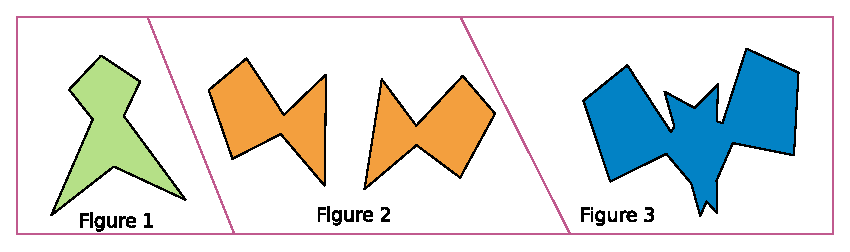
\includegraphics[width=14.5cm]{miroir} \end{center}

\begin{partie}
Observe les trois figures ci‑dessus :
\begin{enumerate}
 \item Quel est leur point commun ?
 
Comment peux‑tu le mettre en évidence ?
 \item Dans des publicités ou des magazines, trouve des images ou des logos qui ont la même propriété.
 \end{enumerate}
\end{partie}

\begin{minipage}[c]{0.54\linewidth}
\begin{partie}
À l'aide de papier calque, complète la figure ci‑contre avec un minimum de tracés pour que la droite d soit son \textbf{axe de symétrie}.
\end{partie}
\end{minipage}
\begin{minipage}[c]{0.44\linewidth}
\begin{center} 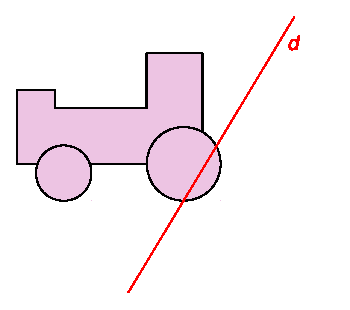
\includegraphics[width=4.5cm]{train} \end{center}
\end{minipage} \\

\end{activite}

%%%%%%%%%%%%%%%%%%%%%%%%%%%%%%%%%%%%%%%%%%%%%%%%%%%%%%%%%%%%%%%%%

\begin{activite}[Le symétrique dans l'œil]

\begin{center}
\begin{tabularx}{1.05\linewidth}{XXXX}
\begin{center} 
\includegraphics[width=3cm]{oeil1} \end{center} & \begin{center} 
\includegraphics[width=2.5cm]{oeil2} \end{center} & \begin{center} 
\includegraphics[width=3.2cm]{oeil3} \end{center} & \begin{center} 
\includegraphics[width=3.5cm]{oeil4} \end{center} \\
\begin{center} Figure 1 \end{center} & \begin{center} Figure 2 \end{center} & \begin{center} Figure 3 \end{center} & \begin{center} Figure 4 \end{center} \\
 \end{tabularx}
 \end{center}

\begin{partie} \label{SymAxCent_acti}
Observe les figures ci-dessus. La figure bleue est‑elle toujours symétrique à la figure orange par rapport à la droite tracée ? Justifie ta réponse en écrivant une phrase.
\end{partie}

\begin{partie}
Reproduis les figures ci‑dessous. Complète‑les à main levée en respectant la symétrie par rapport à la droite d et en tenant compte des remarques faites dans la partie \ref{SymAxCent_acti}.

\begin{minipage}[c]{0.48\linewidth}
\begin{center} 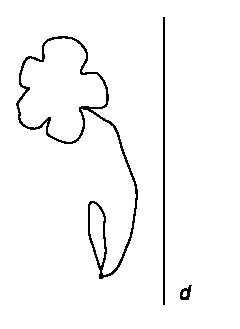
\includegraphics[width=3.5cm]{figure1} \end{center} 
 \end{minipage}
 \begin{minipage}[c]{0.48\linewidth}
 \begin{center} 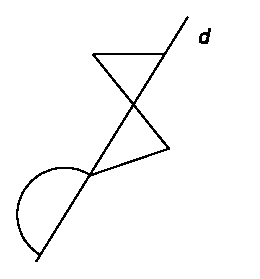
\includegraphics[width=3.5cm]{figure2} \end{center} 
  \end{minipage} \\
\end{partie}

\end{activite}

%%%%%%%%%%%%%%%%%%%%%%%%%%%%%%%%%%%%%%%%%%%%%%%%%%%%%%%%%%%%%%%%%

\begin{activite}[Une droite bien connue]

\begin{minipage}[c]{0.64\linewidth}
\begin{partie}
Sur la figure ci‑contre, quel est le symétrique du point $A$ par rapport à l'axe $d$ ? \\[0.5em]
Trouve les paires de points symétriques par rapport à la droite $d$. Décalque‑les ainsi que la droite $d$.
\end{partie}

\begin{partie}
Quel est le symétrique du point $J$ par rapport à l'axe $d$ ? Y a‑t‑il un autre point qui a la même particularité ?
\end{partie}

\begin{partie}
Sur ton calque, relie les points qui sont symétriques. Que peux-tu dire de la droite $d$ pour ces segments ?
\end{partie}
 \end{minipage}
  \qquad \begin{minipage}[c]{0.30\linewidth}
  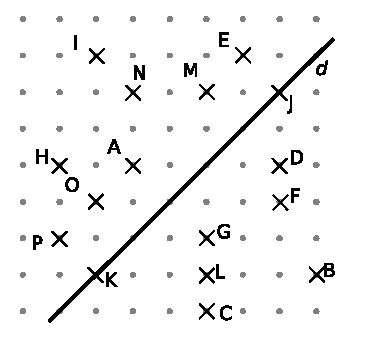
\includegraphics[width=5.5cm]{droite_connue}
  \end{minipage} \\
 

\begin{partie}
Trace le cercle de centre $J$ passant par $A$ et celui de centre $K$ passant par $A$. Que remarques‑tu ?
         
Trace un autre cercle passant par $A$ et $G$. Où doit se situer son centre ?
\end{partie}


\begin{partie}
Sur ton calque, place un point $T$ qui n'est pas sur la droite $d$. Propose deux façons de construire son symétrique $T'$ par rapport à $d$ sans plier le calque.
\end{partie}

\end{activite}

%%%%%%%%%%%%%%%%%%%%%%%%%%%%%%%%%%%%%%%%%%%%%%%%%%%%%%%%%%%%%%%%%

\begin{activite}[Un peu de mesure]

\begin{partie}[Symétrique d'un segment]
\begin{enumerate}
 \item Trace une droite $d$ et un segment $[AB]$. Construis le symétrique du segment $[AB]$ par rapport à la droite $d$.
 \item Compare les mesures des deux segments. Tes camarades obtiennent‑ils la même remarque ?
 
 \begin{minipage}[c]{0.52\linewidth}
 \item Romain avait construit le symétrique $A'B'C'$ du triangle $ABC$ par rapport à l'axe $d$. Malheureusement, sa feuille s'est déchirée et il ne reste que la figure ci‑contre. Romain doit déterminer le périmètre du triangle $ABC$. 
 
Explique comment il peut faire en utilisant uniquement la règle graduée et sans tracé supplémentaire.
  \end{minipage}
   \qquad \begin{minipage}[c]{0.46\linewidth}
  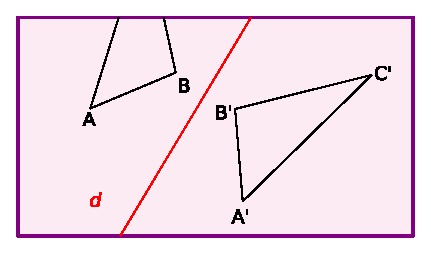
\includegraphics[width=5.5cm]{feuille_Romain}
  \end{minipage} \\
 \end{enumerate}
\end{partie}

\begin{partie}[Symétrique d'un cercle]
\begin{enumerate}
 \begin{minipage}[c]{0.62\linewidth}
 \item Reproduis la figure ci‑contre, place un point $M$ sur le cercle (\phantom{...}) puis construis les points $O'$ et $M'$ symétriques respectifs de $O$ et de $M$ par rapport à $d$.
 
Quelle est la longueur de $[O'M']$ ? Justifie ta réponse.
 \item Construis le symétrique du cercle (\phantom{...}) par rapport à la droite $d$.
  \end{minipage}
   \qquad \begin{minipage}[c]{0.36\linewidth}
  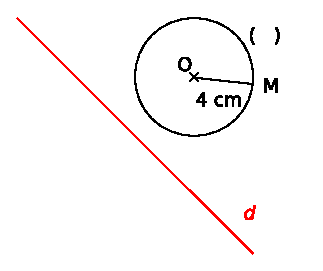
\includegraphics[width=4.5cm]{cercle_sym}
  \end{minipage} \\
 \end{enumerate}
\end{partie}

\end{activite}

%%%%%%%%%%%%%%%%%%%%%%%%%%%%%%%%%%%%%%%%%%%%%%%%%%%%%%%%%%%%%%%%%

\begin{activite}[Symétrique d'une droite]

\begin{minipage}[c]{0.62\linewidth}
\begin{partie}[Droite parallèle à l'axe]
\begin{enumerate}
 \item Trace deux droites parallèles \textcolor{B2}{$d$} et $d_1$ ;
 \item Construis la droite $d_2$ symétrique de la droite $d_1$ par rapport à l'axe \textcolor{B2}{$d$} ;
 \item Que peux‑tu dire des droites $d_1$ et $d_2$ ? Justifie ta réponse.
 \end{enumerate}
\end{partie}
 \end{minipage}
   \qquad \begin{minipage}[c]{0.36\linewidth}
  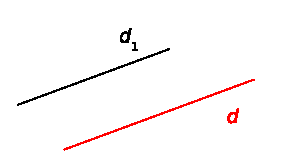
\includegraphics[width=4.5cm]{d1d}
  \end{minipage} \\

\vspace{1em}

\begin{minipage}[c]{0.62\linewidth}
\begin{partie}[Droite perpendiculaire à l'axe]
\begin{enumerate}
 \item Construis deux droites \textcolor{B2}{$d$} et $d_1$ perpendiculaires ;
 \item Place un point $A$ sur la droite $d_1$ et construis son symétrique $A'$ par rapport à l'axe \textcolor{B2}{$d$}. Justifie la position du point $A'$. \\[0.5em]
Que peux-tu dire alors de la droite $d_2$ symétrique de la droite $d_1$ par rapport à l'axe $d$ ?
 \end{enumerate}
\end{partie}
 \end{minipage}
   \qquad \begin{minipage}[c]{0.36\linewidth}
  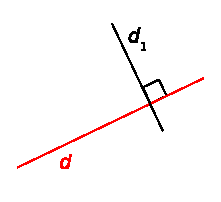
\includegraphics[width=3.5cm]{d1_perp_d}
  \end{minipage} \\

\end{activite}

%%%%%%%%%%%%%%%%%%%%%%%%%%%%%%%%%%%%%%%%%%%%%%%%%%%%%%%%%%%%%%%%%

%%%%%%%%%%%%%%%%%%%%%%%%%%%%%%%%%%%
%%%%%%%%%%%%%%%%%%%%%%%%%%%%%%%%%%%
%MiseEnPage
%%%%%%%%%%%%%%%%%%%%%%%%%%%%%%%%%%%
\newpage
%%%%%%%%%%%%%%%%%%%%%%%%%%%%%%%%%%%
%%%%%%%%%%%%%%%%%%%%%%%%%%%%%%%%%%%



\begin{activite}[Calque et demi-tour]

Mathieu a décalqué le bateau rose puis il l'a fait tourner autour du point $O$ dans le sens de la flèche. Il a dessiné quatre bateaux de couleurs différentes.

\vspace{1em}

\begin{minipage}[c]{0.52\linewidth}
\begin{partie}
Certains bateaux sont à moins d'un demi-tour, d'autres à plus d'un demi-tour du bateau de départ. Peux-tu préciser lesquels ?
\end{partie}

\begin{partie}
Reproduis, sur ton cahier, le bateau rose et le point $O$. À l'aide d'un morceau de papier calque, place un bateau qui soit à moins d'un demi-tour et un autre qui soit à plus d'un demi-tour du bateau de départ.
\end{partie}

\begin{partie} \label{SymAxCentActi2}
Mathieu remarque que lorsqu'il fait tourner le bateau rose autour du point $O$, le point $A$, tout en haut du mât, décrit une ligne qu'il connaît bien. Quelle est cette ligne ? Construis-la sur ton dessin.
\end{partie}
 \end{minipage}
   \quad \begin{minipage}[c]{0.26\linewidth}
  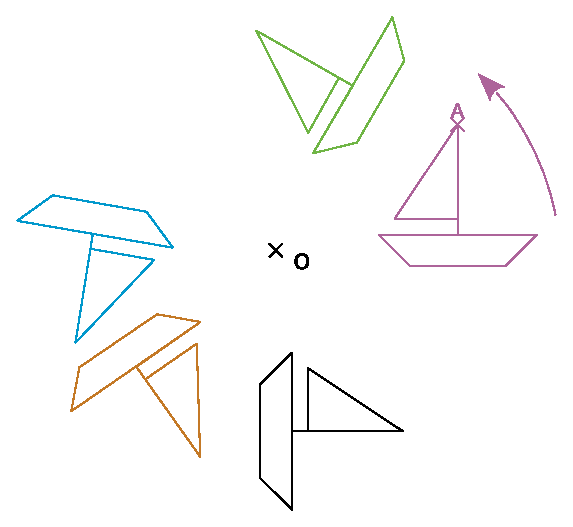
\includegraphics[width=6.7cm]{bateaux}
  \end{minipage} \\

\begin{partie} \label{SymAxCentActi3}
Mathieu aimerait bien construire un bateau qui soit exactement à un demi-tour du bateau rose. Pour savoir où s'arrêter de tourner, Mathieu se dit qu'il faudrait connaître la position exacte du point $A$ après un demi-tour. Construis ce point.
\begin{center} \textbf{\textcolor{H1}{Le demi-tour autour du point $O$ est encore appelé symétrie de centre $O$.}} \end{center}
\end{partie}

\begin{partie}
En t'aidant des parties \ref{SymAxCentActi2} et \ref{SymAxCentActi3}, construis le symétrique du bateau de départ par la symétrie de centre $O$.
\end{partie}

\end{activite}

%%%%%%%%%%%%%%%%%%%%%%%%%%%%%%%%%%%%%%%%%%%%%%%%%%%%%%%%%%%%%%%%%



\begin{activite}[Dans un quadrillage]

\begin{minipage}[c]{0.67\linewidth}
\begin{partie}
Reproduis la figure ci-contre sur ton cahier. \\[0.5em]
Pour aller de $O$ à $A$, on suit la flèche rose puis la verte.
\end{partie}
 \end{minipage}
  \qquad \begin{minipage}[c]{0.36\linewidth}
  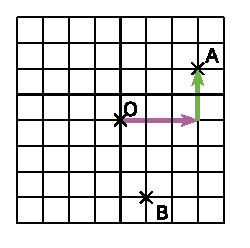
\includegraphics[width=3.7cm]{quadrillageAOB}
  \end{minipage} \\

\begin{partie}
En utilisant du papier calque, construis le symétrique de chaque flèche par rapport à $O$ puis complète les phrases suivantes : 
\begin{itemize}
 \item Le symétrique par rapport à un point d'une flèche de trois carreaux vers la droite est une flèche \ldots ;
 \item Le symétrique par rapport à un point d'une flèche de deux carreaux vers le haut est \ldots.
 \end{itemize}
\end{partie}
                
\begin{partie}
À l'aide des symétriques des flèches rose et verte, place le point $A'$, symétrique du point $A$ par rapport à $O$.
\end{partie}
         
\begin{partie}
En utilisant uniquement le quadrillage et en t'inspirant de la méthode découverte ci-dessus, place le point $B'$ symétrique du point $B$ par rapport à $O$.
\end{partie}

\end{activite}

%%%%%%%%%%%%%%%%%%%%%%%%%%%%%%%%%%%%%%%%%%%%%%%%%%%%%%%%%%%%%%%%%

\begin{activite}[Centre de symétrie]

\begin{partie}
Construis un segment $[RS]$ de 5 cm de longueur. Quel est son centre de symétrie ?
\end{partie}


\begin{partie}
Construis un cercle de centre $O$ et de rayon 3 cm. Quel est son centre de symétrie ?
\end{partie}
         
         
\begin{partie}
Construis une droite $d$. Combien admet-elle de centres de symétrie ?
\end{partie}
         
         
\begin{partie}
Est-il possible de construire un triangle non aplati qui a un centre de symétrie ?
\end{partie}
         
         
\begin{partie}
Place trois points non alignés $A$, $B$ et $O$. Construis les points $C$ et $D$ pour que le quadrilatère $ABCD$ ait le point $O$ comme centre de symétrie.
\end{partie}
        
\vspace{1em}

\begin{minipage}[c]{0.62\linewidth}
\begin{partie}
Sur ton cahier, place trois points $Z$, $V$ et $W$ comme sur la figure ci-contre. Comment construire le point $M$ pour que le quadrilatère $ZVWM$ ait un centre de symétrie ?
\end{partie}         
              
         
\begin{partie}
Construis un hexagone $EFGHIJ$ qui admet un centre de symétrie.
\end{partie}
 \end{minipage}
  \qquad \begin{minipage}[c]{0.36\linewidth}
  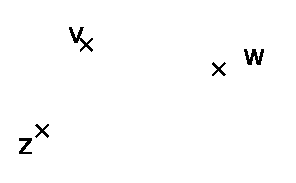
\includegraphics[width=4.5cm]{pointsVWZ}
  \end{minipage} \\

\end{activite}

%%%%%%%%%%%%%%%%%%%%%%%%%%%%%%%%%%%%%%%%%%%%%%%%%%%%%%%%%%%%%%%%%


\exercicesbase
\begin{colonne*exercice}

\serie{Symétrie axiale}

\begin{exercice}[Figures symétriques ?]
Dans chaque cas, indique si les figures verte et orange sont symétriques par rapport à une droite.
\begin{center} 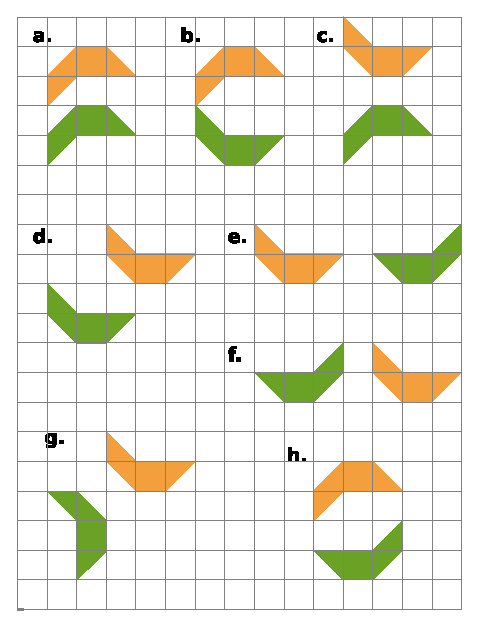
\includegraphics[width=7.9cm]{figures_sym} \end{center}
\end{exercice}


\begin{exercice}[Figures symétriques ? (bis)]
Dans chaque cas, indique si les figures mauve et bleue sont symétriques par rapport à une droite.
\begin{center} 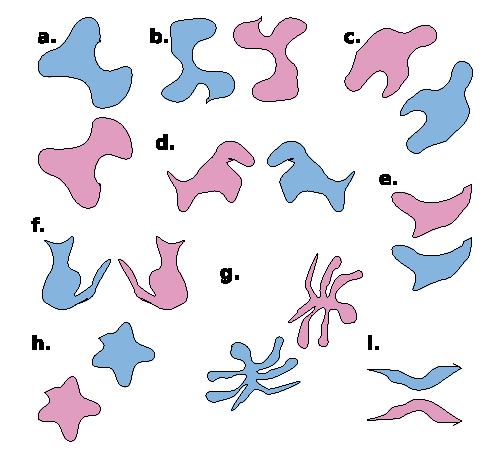
\includegraphics[width=8.1cm]{figures_sym2} \end{center}
\end{exercice}


\begin{exercice}[Erreurs à trouver]
Pourquoi les figures ocre et verte ne sont-elles pas symétriques par rapport à la droite $d$ ?
\begin{center} 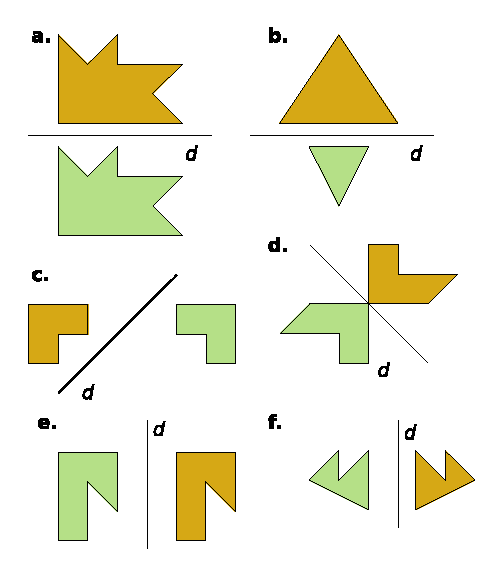
\includegraphics[width=7.9cm]{figures_erreurs} \end{center}
\end{exercice}


\begin{exercice}[Figure à plier]
\begin{minipage}[c]{0.62\linewidth}
Sur du papier calque, trace une droite rouge. Cette droite partage ton calque en deux.

Dessine un motif en t'inspirant du dessin ci‑contre sur la première moitié du calque, puis plie ton calque et complète ton dessin pour que ta figure soit symétrique par rapport à l'axe noir.
 \end{minipage} \hfill%
 \begin{minipage}[c]{0.36\linewidth}
 \begin{center} 
\includegraphics[width=1.7cm]{papillon} \end{center}
  \end{minipage} \\
\end{exercice}


\begin{exercice}[Jeu des différences]
Retrouve les erreurs qui se sont glissées sur ces deux figures pour qu'elles soient parfaitement symétriques par rapport à la droite rouge.
\begin{center} 
\includegraphics[width=5cm]{jeu_differences} \end{center}
\end{exercice}


\begin{exercice}[Points symétriques]
\begin{enumerate}
 \item Sur la figure ci‑dessous, cite les couples de points qui sont symétriques par rapport à l'axe rouge. \\[0.3em]
 \begin{center} 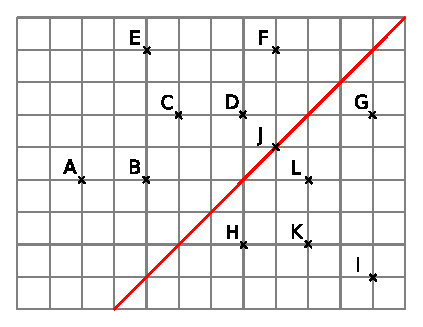
\includegraphics[width=6.9cm]{quadrillage_axerouge} \end{center}
 \item Fais trois phrases du type : « L'axe rouge est l'axe de symétrie du segment \ldots ».
 \item Reproduis cette figure et complète‑la pour que chaque point ait un symétrique.
 \end{enumerate}
\end{exercice}


\begin{exercice}[Cases croisées]
Reproduis et colorie le minimum de cases pour que l'axe rouge soit un axe de symétrie.
 \begin{center} 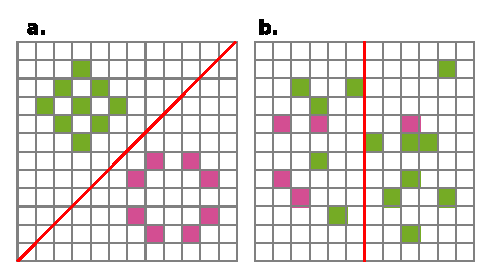
\includegraphics[width=8.1cm]{cases_croisees} \end{center}
\end{exercice}


\begin{exercice}[Frise]
Reproduis la figure ci‑dessous puis trace son symétrique par rapport à l'axe rouge. 
 \begin{center} 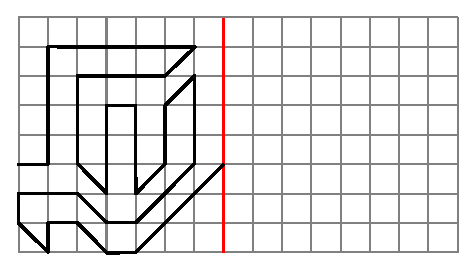
\includegraphics[width=7.9cm]{frise} \end{center}
\end{exercice}


\begin{exercice}
Reproduis puis trace le symétrique de chaque figure par rapport à $d$.

\begin{minipage}[c]{0.48\linewidth}
 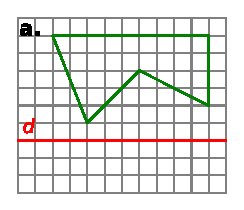
\includegraphics[width=3.7cm]{repro_d1}
 \end{minipage} \hfill%
 \begin{minipage}[c]{0.48\linewidth}
 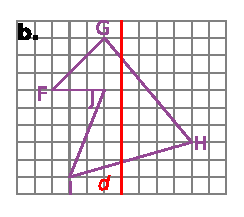
\includegraphics[width=3.7cm]{repro_d2}
  \end{minipage} \\
 \begin{minipage}[c]{0.48\linewidth}
 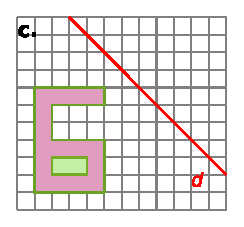
\includegraphics[width=3.7cm]{repro_d3}
 \end{minipage} \hfill%
 \begin{minipage}[c]{0.48\linewidth}
 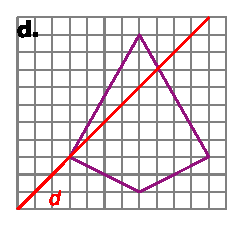
\includegraphics[width=3.7cm]{repro_d4}
 \end{minipage} \\
\end{exercice}


%%%%%%%%%%%%%%%%%%%%%%%%%%%%%%%%%%%
%%%%%%%%%%%%%%%%%%%%%%%%%%%%%%%%%%%
%MiseEnPage
%%%%%%%%%%%%%%%%%%%%%%%%%%%%%%%%%%%
\newpage
%%%%%%%%%%%%%%%%%%%%%%%%%%%%%%%%%%%
%%%%%%%%%%%%%%%%%%%%%%%%%%%%%%%%%%%

\begin{exercice}[Symétrique d'un point]
\begin{enumerate}
 \item Reproduis une figure similaire à celle ci‑dessous :
 \begin{center} 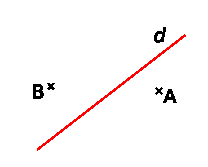
\includegraphics[width=2.8cm]{pointsABd} \end{center}
 \item Construis le symétrique par rapport à $d$ du point :
 \begin{itemize}
  \item $A$ à la règle et l'équerre ;
  \item $B$ au compas.
  \end{itemize}   
 \item Soit $H$ le point d'intersection de $(AB)$ avec $d$. Que dire de son symétrique par rapport à $d$ ?
 \end{enumerate} 
\end{exercice}


\begin{exercice}[Symétrique d'un triangle]
\begin{minipage}[c]{0.52\linewidth}
\begin{enumerate}
 \item Reproduis une figure similaire à celle ci-contre ;
 \item Construis au compas le symétrique du triangle $GHI$ par rapport à $d$.
 \end{enumerate}
 \end{minipage} \hfill%
 \begin{minipage}[c]{0.44\linewidth}
  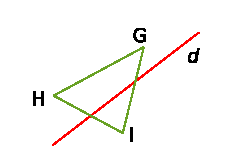
\includegraphics[width=3cm]{triangleGHId}
   \end{minipage} \\
\end{exercice}


\begin{exercice}[Symétrique d'un cercle]
\begin{enumerate}
 \item Trace un cercle $\mathcal{C}$ de centre $G$ et de rayon 5 cm. Place deux points $A$ et $B$ sur ce cercle non diamétralement opposés.
 \item Trace le symétrique de $\mathcal{C}$ par rapport à $(AB)$.
 \item Par quels points passent les deux cercles ? Justifie.
 \item Que se passe‑t‑il si $A$ et $B$ sont diamétralement opposés ?
 \end{enumerate}
\end{exercice}


\begin{exercice}[Symétrique d'une figure]
\begin{minipage}[c]{0.44\linewidth}
\begin{enumerate}
 \item Reproduis une figure similaire à celle ci‑contre ;
 \item À l'aide d'une règle et d'une équerre, trace le symétrique de cette figure par rapport à la droite $(AB)$.
 \end{enumerate}
 \end{minipage} \hfill%
 \begin{minipage}[c]{0.52\linewidth}
  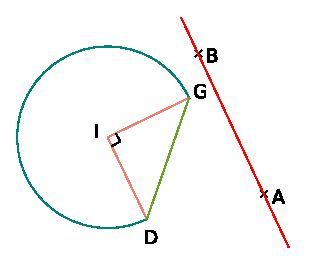
\includegraphics[width=4.5cm]{figure_droiteAB}
   \end{minipage} \\
\end{exercice}

%%%%%%%%%%%%%%%%%%%%%%%%%%%%%%%%%%%
%%%%%%%%%%%%%%%%%%%%%%%%%%%%%%%%%%%
%MiseEnPage
%%%%%%%%%%%%%%%%%%%%%%%%%%%%%%%%%%%
\columnbreak
%%%%%%%%%%%%%%%%%%%%%%%%%%%%%%%%%%%
%%%%%%%%%%%%%%%%%%%%%%%%%%%%%%%%%%%

\begin{exercice}[À propos des distances]
\begin{enumerate}
 \item Reproduis une figure similaire à celle ci‑dessous : 
 \begin{center} 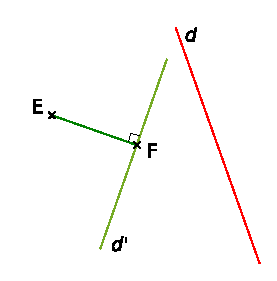
\includegraphics[width=4.7cm]{distances} \end{center}
 \item Trace le symétrique de $[EF]$ par rapport à $d$. On le note $[E'F']$. Que peux‑tu dire de la longueur de $[E'F']$ ? Justifie.
 \item Que peux‑tu dire du symétrique de $d'$ par rapport à $d$ ? Trace alors ce symétrique.
 \item Que peux‑tu dire du symétrique du cercle de diamètre $[EF]$ par rapport à $d$ ? Justifie.
 \end{enumerate}
\end{exercice}


\begin{exercice}[À propos de l'alignement]
\begin{enumerate}
 \item Trace une droite $d$. Place trois points $A$, $B$ et $C$ alignés qui n'appartiennent pas à $d$ ;
 \item Construis les points $A'$, $B'$ et $C'$ symétriques respectifs de $A$, $B$ et $C$ par rapport à $d$ ;
 \item Que dire des points $A'$, $B'$ et $C'$ ? Justifie.
 \end{enumerate}
\end{exercice}


\begin{exercice}[À propos des milieux]
\begin{enumerate}
 \item Effectue le programme de construction :
 \begin{itemize}
  \item Trace un segment $[KL]$ de longueur 7 cm ;
  \item Place le point $M$ sur $[KL]$ tel que $LM = 2$ cm ;
  \item Place le milieu $I$ de $[ML]$ ;
  \item Place le milieu $J$ de $[MK]$ ;
  \item Trace la droite $(d)$, passant par $M$ et perpendiculaire à $(KL)$ ;
  \item Trace le symétrique $I'$ de $I$ par rapport à $(d)$ et le symétrique $J'$ de $J$ par rapport à $(d)$.
  \end{itemize}
 \item Calcule, en justifiant, la longueur du segment $[I'J']$.
 \end{enumerate}
\end{exercice}

%%%%%%%%%%%%%%%%%%%%%%%%%%%%%%%%%%%
%%%%%%%%%%%%%%%%%%%%%%%%%%%%%%%%%%%
%MiseEnPage
%%%%%%%%%%%%%%%%%%%%%%%%%%%%%%%%%%%
\newpage
%%%%%%%%%%%%%%%%%%%%%%%%%%%%%%%%%%%
%%%%%%%%%%%%%%%%%%%%%%%%%%%%%%%%%%%

\begin{exercice}[À propos du périmètre]
\begin{enumerate}
 \item Trace un triangle $ABC$ tel que $AB = 5$ cm, $AC = 6$ cm et $BC = 9$ cm sur une feuille blanche.
Trace une droite $d$ parallèle à $(BC)$.
 \item Trace au compas le symétrique du triangle $ABC$ par rapport à $d$. On le note $A'B'C'$.
 \item Quel est le périmètre du triangle $A'B'C'$ ? 
 \end{enumerate}
\end{exercice}


\begin{exercice}[Sans axe]
Les deux figures ci-dessous sont symétriques par rapport à une droite.
 \begin{center} 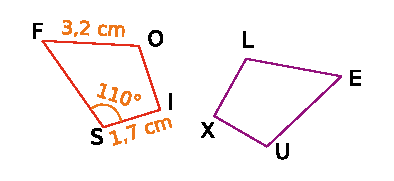
\includegraphics[width=5.9cm]{sans_axe} \end{center}
 \begin{enumerate}
 \item Reproduis et complète le tableau suivant.
 \begin{center}
  \begin{tabularx}{0.9\linewidth}{|c|*{6}{>{\centering\arraybackslash}X|}}
  \hline
\rowcolor{J1} Points & $F$ & $O$ & $I$ & $S$ \\ \hline
\rowcolor{C3} Symétriques & & & & \\ \hline
 \end{tabularx}
 \end{center}
 \vspace{0.3cm}
Tu justifieras ensuite chaque réponse.
 \item Quelle est la longueur du segment $[LE]$ ?
 \item Quelle autre longueur peux‑tu déterminer ?
 \item Quelle est la mesure de l'angle $\widehat{XUE}$ ?
 \item Écris deux autres égalités de mesure d'angles.
 \end{enumerate}
\end{exercice}


\begin{exercice}[À la recherche de l'axe]
Dans chaque cas, décalque les deux figures puis trace l'axe de symétrie. (Tu expliqueras comment tu fais sans plier le calque.)
 \begin{center} 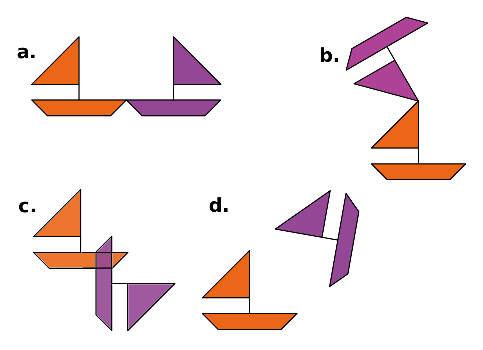
\includegraphics[width=8cm]{bateaux_colores} \end{center}
\end{exercice}

%%%%%%%%%%%%%%%%%%%%%%%%%%%%%%%%%%%%%%%%%%%%%%%%%%%%%%%%%%%%%%%%%%%%

\serie{Symétrie centrale}

\begin{exercice}
À l'aide de la règle graduée, retrouve, sur la figure ci-dessous, toutes les paires de points qui semblent symétriques par rapport au point $N$ : 
 \begin{center} 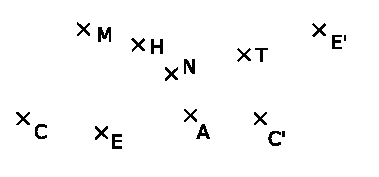
\includegraphics[width=5.8cm]{many_points} \end{center}
\end{exercice}


\begin{exercice}
Reforme des phrases correctes en associant les bonnes cases et recopie-les sur ton cahier :
\begin{center}
\renewcommand*\tabularxcolumn[1]{>{\centering\arraybackslash}m{#1}}
\begin{ttableau}{\linewidth}{3}
 \cline{1-1}\cline{3-3}
 \small{$A'$ est le symétrique du point $A$ par rapport au point $O$ donc \ldots} & & \small{$A'$ est le milieu du segment $[OA]$.} \\  \cline{1-1}\cline{3-3}
 \small{$O$ est l'image du point $A$ par la symétrie de centre $A'$ donc \ldots} & & \small{$A$ est le milieu du segment $[OA']$.} \\  \cline{1-1}\cline{3-3}
 \small{Le point $A'$ se transforme en $O$ par la symétrie de centre $A$ donc \ldots} & & \small{$O$ est le milieu du segment $[AA']$.} \\  \cline{1-1}\cline{3-3}
 \end{ttableau}
 \end{center}
\end{exercice}


\begin{exercice}
Dans chaque cas, reproduis la lettre sur du papier quadrillé et construis son symétrique par rapport au point $G$ :
 \begin{center} 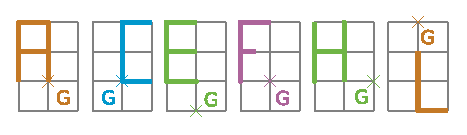
\includegraphics[width=7.7cm]{lettresG} \end{center}
\end{exercice}


\begin{exercice}
Sur ton cahier, reproduis la figure ci-dessous et construis les symétriques des points $P$, $R$ et $O$ par rapport au point $F$ :
 \begin{center} 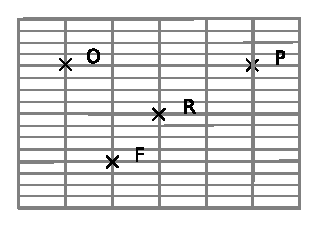
\includegraphics[width=5cm]{cahierFORP} \end{center}
\end{exercice}


\begin{exercice}
Sur ton cahier, reproduis la figure et construis le symétrique du mot MAT par rapport au point $R$ puis le symétrique du mot obtenu par rapport à la droite $d$ :
 \begin{center} 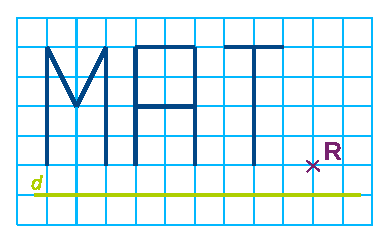
\includegraphics[width=6.3cm]{MAT} \end{center}
\end{exercice}


\begin{exercice}
Dans chaque cas, reproduis la figure et construis le point $D$, symétrique du point $A$ par rapport au point $C$ puis le point $E$, symétrique du point $C$ par rapport au point $B$ :
\begin{colenumerate}{2}
 \item 
 
 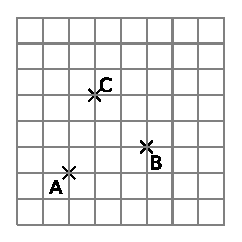
\includegraphics[width=3.7cm]{symCAB1}
 \item 
 
 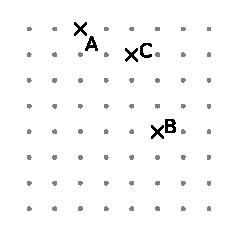
\includegraphics[width=3.7cm]{symCAB2}
 \end{colenumerate}
\end{exercice}


\begin{exercice}

\begin{minipage}[c]{0.48\linewidth}
Reproduis séparément chaque triangle sur du papier quadrillé et construis son symétrique par rapport au point $S$ :
 \end{minipage} \hfill%
 \begin{minipage}[c]{0.48\linewidth}
 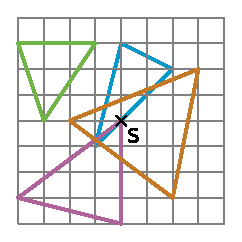
\includegraphics[width=3.7cm]{triangles_symS}
 \end{minipage} \\
\end{exercice}


\begin{exercice}
Reproduis les figures ci-dessous sur du papier quadrillé et construis le symétrique de chacune d'elles par rapport au point $H$ :
\begin{colenumerate}{2}
 \item 

 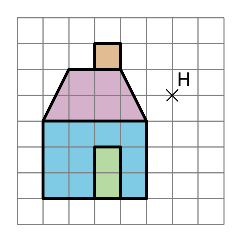
\includegraphics[width=3.7cm]{maison_sym}

 \item
 
 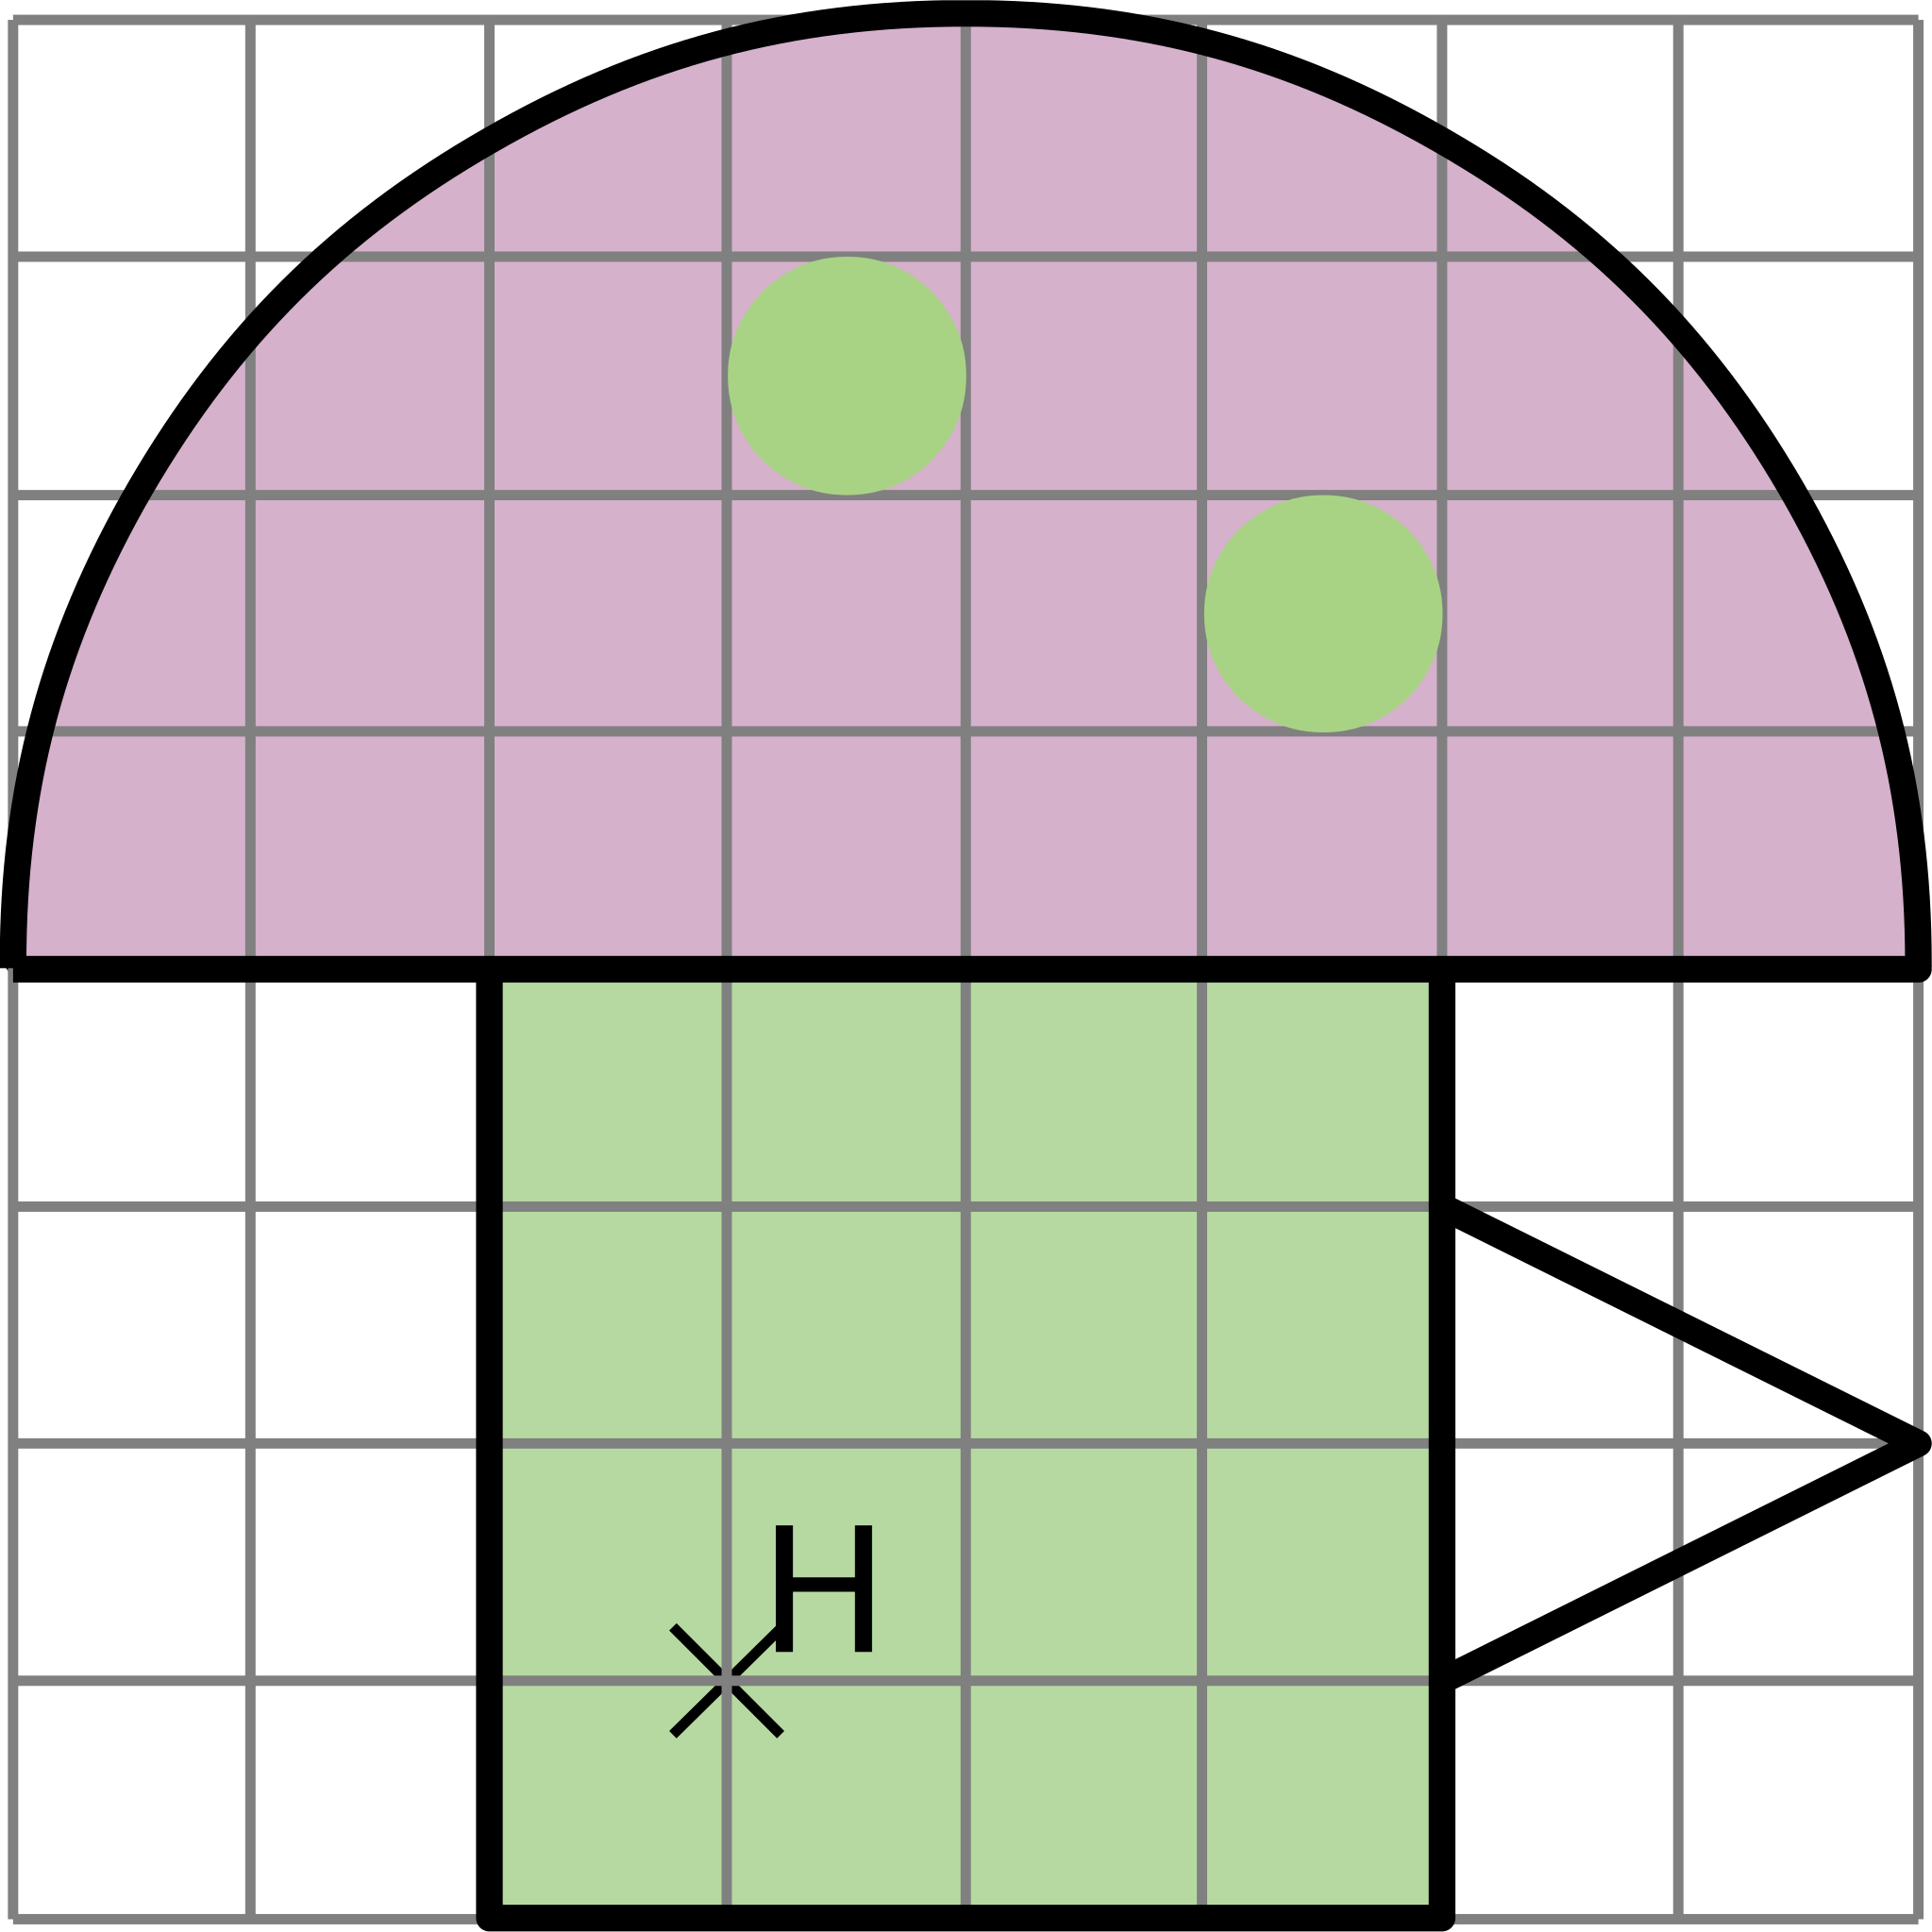
\includegraphics[width=3.7cm]{champignon_sym}
 \end{colenumerate}
\end{exercice}


\begin{exercice}

\begin{minipage}[c]{0.48\linewidth}
Sur la figure ci-contre, $ROSE$ est un carré de centre $H$. Les points $I$, $J$, $K$ et $L$ sont les milieux respectifs des côtés $[RO]$, $[OS]$, $[SE]$ et $[RE]$.
 \end{minipage} \hfill%
\begin{minipage}[c]{0.48\linewidth}
 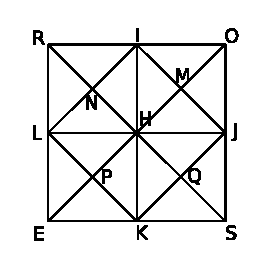
\includegraphics[width=3.7cm]{ROSE}
 \end{minipage} \\
 \begin{enumerate}
  \item Reproduis la figure en prenant $RO = 8$ cm ;
  \item Colorie en jaune le triangle $RNI$ ;
  \item Colorie en rouge le symétrique du triangle $RNI$ par rapport à la droite $(IK)$ puis en orange le symétrique du triangle $RNI$ par rapport à la droite $(LJ)$ ;
  \item Colorie en bleu le symétrique du triangle $RNI$ par rapport au point $N$ puis en vert le symétrique du triangle $RNI$ par rapport au point $H$.
 \end{enumerate}
\end{exercice}


\begin{exercice}
Dans chacun des quatre cas suivants, des élèves ont voulu tracer la figure symétrique du bateau bleu par rapport au point $C$. Les tracés sont-ils exacts ? Explique pourquoi. 
\begin{colenumerate}{2}
 \item 
 
 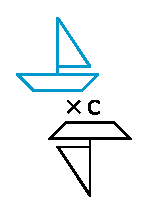
\includegraphics[width=2.3cm]{bateaux_bn1}
 \item 
 
 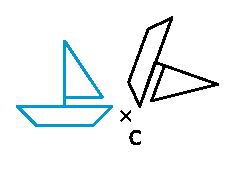
\includegraphics[width=3.7cm]{bateaux_bn2}
 \item 
 
 
\includegraphics[width=3.7cm]{bateaux_bn3}
 \item 
 
 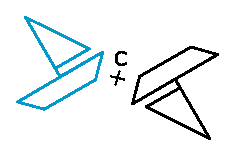
\includegraphics[width=3.7cm]{bateaux_bn4}
 \end{colenumerate}
\end{exercice}


\begin{exercice}
Place trois points $A$, $B$ et $C$ non alignés tels que $AB = 5$ cm et $AC = 3$ cm. Construis, avec seulement la règle graduée, les points $B'$ et $C'$ symétriques respectifs des points $B$ et $C$ par rapport au point $A$.
\end{exercice}


\begin{exercice}
Reproduis la figure ci-dessous et construis, avec la règle non graduée et le compas, les symétriques des points $M$ et $R$ par rapport au point $E$ :
 \begin{center} 
\includegraphics[width=4.4cm]{pointsMER} \end{center}
\end{exercice}


\begin{exercice}
Reproduis chaque figure et construis le symétrique du segment $[AB]$ par rapport au point $S$ :
\begin{colenumerate}{3}
 \item 
 
 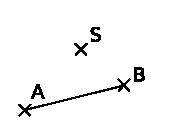
\includegraphics[width=2cm]{pointsSAB_1}
  \item 
 
 \includegraphics[width=2cm]{pointsSAB_2}
  \item 
 
 \includegraphics[width=2.5cm]{pointsSAB_3}
 \end{colenumerate}
\end{exercice}


\begin{exercice}
Reproduis chaque figure et construis le symétrique de la droite $d$ par rapport au point $U$ :
\begin{colenumerate}{2}
 \item 
 
 \includegraphics[width=3.5cm]{pointsUd}
  \item 
 
 \includegraphics[width=3.5cm]{pointsUd2}
 \end{colenumerate}
\end{exercice}


\begin{exercice}
Reproduis chaque figure en prenant 5 cm pour le rayon du cercle puis construis le symétrique du cercle par rapport au point $T$ :
\begin{colenumerate}{3}
 \item \includegraphics[width=2cm]{cercleKT1}
 \item \includegraphics[width=2cm]{cercleKT2}
 \item \includegraphics[width=1.4cm]{cercleKT3}
 \end{colenumerate}
\end{exercice}


\begin{exercice}
Construis un triangle $EFG$ rectangle en $E$ tel que $EF = 3$ cm et $EG = 5$ cm.
\begin{enumerate}
 \item Place le point $M$ milieu du segment $[EF]$ puis construis les points $E_1$, $F_1$ et $G_1$ symétriques respectifs des points $E$, $F$ et $G$ par rapport au point $M$ ;
 \item Construis les points $E_2$, $F_2$ et $G_2$ images respectives des points $E_1$, $F_1$ et $G_1$  par la symétrie de centre $E$ ;
 \item Place le point $K$ milieu du segment $[FG]$ puis construis les points $E_3$, $F_3$ et $G_3$ symétriques respectifs des points $E$, $F$ et $G$ par rapport au point $K$ ;
 \item Les points $E_3$, $F_3$ et $G_3$ sont les images respectives des points $E_2$, $F_2$ et $G_2$ par la symétrie de centre $O$. Quelle semble être la position de ce point $O$ ? Place-le sur ta figure.
 \end{enumerate}
\end{exercice}


\begin{exercice}[Figures complexes]
\begin{enumerate}
 \item Reproduis la figure ci-dessous, en haut à gauche avec $AB = 8$ cm et $AD = 5$ cm. Le point $E$ est le milieu du segment $[AB]$. 
 \begin{center} \includegraphics[width=5.2cm]{fig_complexes} \end{center}
 \item Construis le symétrique de cette figure par rapport au point $B$.
 \end{enumerate}
\end{exercice}


\begin{exercice}
Construis un rectangle $MATH$ tel que $MA = 5$ cm et $AT = 7$ cm puis place le point $E$ sur le côté $[AT]$ tel que $AE = 2$ cm. Construis en rouge le symétrique du rectangle $MATH$ par rapport au point $E$.
\end{exercice}


\begin{exercice}
Parmi les cartes ci-dessous, quelles sont celles qui possèdent un centre de symétrie ? 
 \begin{center} \includegraphics[width=7.7cm]{cartes_poker1} \end{center}
\end{exercice}

%%%%%%%%%%%%%%%%%%%%%%%%%%%%%%%%%%%
%%%%%%%%%%%%%%%%%%%%%%%%%%%%%%%%%%%
%MiseEnPage
%%%%%%%%%%%%%%%%%%%%%%%%%%%%%%%%%%%
\newpage
%%%%%%%%%%%%%%%%%%%%%%%%%%%%%%%%%%%
%%%%%%%%%%%%%%%%%%%%%%%%%%%%%%%%%%%

\begin{exercice}
Marine affirme que toutes les cartes ci-dessous possèdent un centre de symétrie. A-t-elle raison ? Justifie ta réponse.
 \begin{center} \includegraphics[width=7.7cm]{cartes_poker2} \end{center}
\end{exercice}


\begin{exercice}
Reproduis les lettres ci-dessous puis, trace en vert l'axe (ou les axes) de symétrie et en rouge le centre de symétrie de chaque lettre lorsqu'il(s) existe(nt) :
 \begin{center} \includegraphics[width=7.4cm]{lettres_grandes} \end{center}
\end{exercice}


\begin{exercice}
Sur la figure ci-dessous, le point $B$ est le symétrique du point $A$ par rapport à $O$ :
 \begin{center} \includegraphics[width=7.9cm]{quadrillageABCDE} \end{center}
\begin{enumerate}
 \item Reproduis la figure ci-dessus puis place le point $O$ ;
 \item En t'aidant du quadrillage, place les points $C'$, $D'$ et $E'$ symétriques respectifs des points $C$, $D$ et $E$ par rapport à $O$.
 \end{enumerate}
\end{exercice}


\begin{exercice}
Reproduis puis complète la figure ci-dessous pour que $O$ soit un centre de symétrie de celle-ci :
 \begin{center} \includegraphics[width=6.9cm]{quadrillage_figsym} \end{center}
\end{exercice}


\begin{exercice}
Reproduis puis colorie le minimum de cases pour que chacune des figures ci-dessous admette le point $O$ pour centre de symétrie :

\begin{minipage}[c]{0.48\linewidth}
\includegraphics[width=3.7cm]{carreaux_colores1}
 \end{minipage} \hfill%
\begin{minipage}[c]{0.48\linewidth}
 \includegraphics[width=3.7cm]{carreaux_colores2}
 \end{minipage} \\

\end{exercice}


\begin{exercice}
Reproduis la figure ci-dessous et complète-la de telle sorte que le centre du rectangle vert soit le centre de symétrie de la figure :
 \begin{center} \includegraphics[width=7.9cm]{fig_completer} \end{center}
\end{exercice}


\begin{exercice}[Nombres et centre de symétrie]
Christian a écrit les chiffres comme ci-dessous :
 \begin{center} \includegraphics[width=7.7cm]{nombres_grands} \end{center}
 \begin{enumerate}
  \item Il dit : « Si je fais le double du produit de 17 par 29, j'obtiens le plus grand nombre de trois chiffres différents qui possède un centre de symétrie. ». A-t-il raison ? 
  \item Trouve le plus petit nombre de trois chiffres différents dont l'écriture possède un centre de symétrie. Écris ce nombre et place le centre de symétrie.
  \end{enumerate}
\end{exercice}


\begin{exercice}
Soit un angle $\widehat{BAD}$ mesurant $120^\circ$ tel que $AB = 4$ cm et $AD = 5$ cm. Soit $C$ un point tel que le quadrilatère non croisé formé par les points $A$, $B$, $C$ et $D$ admette un centre de symétrie.
\begin{enumerate}
 \item Trace une figure à main levée.
 \item Combien y a-t-il de positions possibles pour le point $C$ ? Pour chaque cas, indique la position du centre de symétrie.
 \item Trace autant de figures qu'il y a de centres de symétrie et indique pour chaque cas le nom et la nature du quadrilatère ainsi construit.
 \end{enumerate}
\end{exercice}


\begin{exercice}
Éric a commencé la phrase suivante :
 \begin{center} « Le symétrique par rapport à $O$ d'un triangle isocèle est ... . ». \end{center}
 \begin{enumerate}
  \item Peux-tu compléter sa phrase ?
  \item Éric a oublié de justifier sa phrase. Fais-le pour lui.
  \item Écris deux autres phrases du même type en n'oubliant pas de justifier.
  \end{enumerate}
\end{exercice}


\begin{exercice}
On a tracé, à main levée, deux figures symétriques par rapport à $O$ :
 \begin{center} \includegraphics[width=7.9cm]{polygones_sym} \end{center}
\begin{enumerate}       
 \item Indique le symétrique par rapport à $O$ de chaque sommet du polygone $ABCDE$.
 \item Donne la longueur du segment $[PK]$. Justifie ta réponse.
 \item Donne la mesure de l'angle $\widehat{NPK}$. Justifie ta réponse.
 \item De quelles autres informations disposes-tu  concernant le polygone $KLMNP$ ? Pourquoi ?
 \end{enumerate}
\end{exercice}

%%%%%%%%%%%%%%%%%%%%%%%%%%%%%%%%%%%
%%%%%%%%%%%%%%%%%%%%%%%%%%%%%%%%%%%
%MiseEnPage
%%%%%%%%%%%%%%%%%%%%%%%%%%%%%%%%%%%
\columnbreak
%%%%%%%%%%%%%%%%%%%%%%%%%%%%%%%%%%%
%%%%%%%%%%%%%%%%%%%%%%%%%%%%%%%%%%%

\begin{exercice}[Histoire d'angles]
\begin{enumerate}
 \item Construis un angle $\widehat{xOy}$ mesurant $74^\circ$ puis place un point $A$ sur $[Ox)$ et un point $B$ sur $[Oy)$ ;
 \item Construis les points $C$ et $D$ symétriques respectifs de $B$ et de $O$ par rapport à $A$ ;
 \item Sans utiliser le rapporteur, mais en justifiant les réponses, donne la mesure de l'angle $\widehat{CDA}$ et compare les mesures des angles $\widehat{BAO}$ et $\widehat{DAC}$ ;
 \item Que peut-on dire des droites $(BD)$ et $(CO)$ ? Justifie ta réponse.
 \end{enumerate}
\end{exercice}


\begin{exercice}[Symétrie et périmètre]
\begin{enumerate}
 \item Trace un triangle $ABC$, isocèle en $A$ tel que $AB = 6$ cm et $BC = 3$ cm. Place le point $I$, milieu du segment $[BC]$ ;
 \item Construis le point $D$ symétrique du point $A$ par rapport à $I$ ;
 \item Donne les longueurs $DB$ et $DC$ puis le périmètre de $ABDC$ ;
 \item Quelle est la nature du quadrilatère $ABDC$ ? Justifie ta réponse.
 \end{enumerate}
\end{exercice}


\begin{exercice}
$ABC$ est un triangle tel que $AB = 4$ cm, $AC = 5$ cm et $BC = 6$ cm. $I$ désigne le milieu de $[AB]$ et $D$ le symétrique de $C$ par rapport à $I$.
\begin{enumerate}
 \item Construis la figure.
 \item Sans mesurer, mais en justifiant tes réponses, donne les mesures AD et BD.
 \end{enumerate}
\end{exercice}

\end{colonne*exercice}


\exercicesappr
\begin{colonne*exercice}

\begin{exercice}[Coloriage]
Reproduis et colorie le minimum de cases pour que la figure obtenue soit symétrique par rapport aux deux axes rouges :
\begin{center} \includegraphics[width=4.2cm]{coloriage_carre} \end{center}
\end{exercice}


\begin{exercice}[Une nouvelle construction]
\begin{enumerate}
 \item Trace à main levée une droite $d$ puis place deux points $M$ et $N$ sur $d$ et un point $B$ n'appartenant pas à $d$ ;
 \item Place, toujours à main levée, le point $B'$ symétrique de $B$ par rapport à $d$ ;
 \item Que peux‑tu dire de $MB$ et $MB'$ ? Justifie ta réponse et code la figure ;
 \item Que peux‑tu dire de $NB$ et $NB'$ ? Justifie ta réponse et code la figure ;
 \item Déduis‑en une méthode de construction du point $B'$ avec tes instruments de géométrie ;
 \item Trace la figure avec tes instruments de géométrie.
 \end{enumerate}
\end{exercice}


\begin{exercice}[L'axe invisible]
\begin{center} \includegraphics[width=7.2cm]{axe_invisible} \end{center}
Reproduis la figure ci‑dessus. Les points $C'$ et $D'$ sont les symétriques respectifs des points $C$ et $D$ par rapport à un axe invisible. \\[0.5em]
Construis les symétriques du cercle orange et du quadrilatère bleu par rapport à cet axe invisible.
\end{exercice}


\begin{exercice}[Mandala]
\begin{enumerate}
 \item Dessine un cercle de rayon 6 cm et deux de ses diamètres perpendiculaires. Tu obtiens quatre points sur le cercle. Trace tous les axes de symétrie de cette nouvelle figure. Tu obtiens de nouveaux points sur le cercle.
 \item Quel polygone obtiens‑tu en reliant tous ces points ? Combien a‑t‑il d'axes de symétrie ? Trace‑les tous.
 \item Poursuis en traçant un cercle de rayon 3 cm de même centre que celui de 6 cm. Reproduis le motif comme indiqué sur la figure 1 puis termine la construction et le coloriage en faisant des symétries successives par rapport aux axes (voir figure 2).
 \end{enumerate}
 \begin{minipage}[c]{0.48\linewidth}
 \includegraphics[width=4cm]{mandala1}
 \end{minipage} \hfill%
 \begin{minipage}[c]{0.48\linewidth}
 \includegraphics[width=4cm]{mandala2} 
  \end{minipage} \\
\begin{minipage}[c]{0.48\linewidth}
\begin{center} figure 1 \end{center}
 \end{minipage} \hfill%
 \begin{minipage}[c]{0.48\linewidth}
\begin{center} figure 2 \end{center}
  \end{minipage} \\
\end{exercice}


\begin{exercice}[Sans figure]
Melinda a réalisé une superbe figure et son symétrique. Malheureusement, elle a perdu sa feuille, mais sur son cahier, elle avait pris la précaution de faire le tableau suivant :
\begin{center}
\begin{tabularx}{0.9\linewidth}{|c|X|X|X|X|X|X|}
\hline
Points & E & T & R & S & A & C \\ \hline
Symétriques & V & J & I & S & Z & D\\ \hline
 \end{tabularx}
 \end{center}
Frédérique lui fait remarquer qu'avec un tel tableau, on peut obtenir des indications sans avoir besoin de la figure.
\begin{enumerate}
 \item Quel est le centre de la symétrie ?
 \item On sait que $ET = 3,4$ cm et $ZD = 5,1$ cm. Donne les longueurs $AC$ et $VJ$. Justifie.
 \item $RSA$ est un triangle équilatéral de 3 cm de côté. Quel autre triangle équilatéral est-on certain d'avoir sur la figure ? Justifie.
 \item On sait que $VJ = JI$. Quelle est la nature du triangle $ETR$ ? Pourquoi ?
 \end{enumerate}
\end{exercice}


\begin{exercice}[Symétrie et repère]
\begin{enumerate}
 \item Dessine un repère d'origine $O$ ayant pour unité le centimètre.
 \item Place les points : $I (1 ; 0)$ ; $A (2 ; 3)$ ; $B (6 ; - 1)$ ; $C (7 ; 3)$ ; $D (- 1 ; 1)$ ; $E (3 ; 0)$.
 \item Construis les points $F$, $G$, $H$ et $K$, symétriques respectifs de $A$, $B$, $C$ et $D$ par rapport à $O$.
 \item Donne les coordonnées de $F$, $G$, $H$ et $K$. Que remarques-tu ? \label{SymAxCent_approf}
 \item Donne les coordonnées des symétriques par rapport à $O$ des points $T (4 ; - 5)$ et $U (5 ; 0)$ sans les placer dans le repère.
 \item Place les points $M$, $N$, $P$ et $R$, symétriques respectifs des points $A$, $B$, $C$ et $D$ par rapport à $E$.
 \item Donne les coordonnées de $M$, $N$, $P$ et $R$. La propriété de la question \ref{SymAxCent_approf}. se vérifie-t-elle ici ? À quelle condition fonctionne-t-elle ?
 \end{enumerate}
\end{exercice}


\begin{exercice}
Reproduis la figure ci-dessous :
\begin{center} \includegraphics[width=3cm]{croixAOBd} \end{center}
\begin{enumerate}
 \item Construis les points $E$ et $F$, symétriques respectifs de $A$ et $B$ par rapport à $O$.
 \item Que peut-on dire des droites $(AB)$ et $(EF)$ ? Justifie ta réponse.
 \item Démontre que les droites $d$ et $(EF)$ sont perpendiculaires.
 \end{enumerate}
\end{exercice}


\begin{exercice}[Médiatrice et symétrie]
\begin{enumerate}
 \item Trace trois droites $d_1$, $d_2$ et $d_3$, concourantes en un point $O$ puis place :
 \begin{itemize}
  \item Sur $d_1$, $A$ et $A'$ tels que $OA = OA' = 3$ cm ;
  \item Sur $d_2$, $B$ et $B'$ tels que $OB = OB' = 4$ cm ;
  \item Sur $d_3$, $C$ et $C'$ tels que $OC = OC' = 5$ cm.
  \end{itemize}
 \item Démontre que $(B'C')$ et $(BC)$ sont parallèles.
 \item Construis la médiatrice d du segment $[BC]$.
 \item Démontre que $d$ est perpendiculaire à $(B'C')$.
 \end{enumerate}
\end{exercice}


\begin{exercice}[Pentagone et hexagone]
\underline{PARTIE A}
\begin{enumerate}
 \item Sur un cercle de centre $O$ et de rayon 4 cm, place un point $A$ puis quatre autres points distincts : $B$, $C$, $D$ et $E$ dans cet ordre tels que les angles $\widehat{AOB}$, $\widehat{BOC}$, $\widehat{COD}$, $\widehat{DOE}$ et $\widehat{EOA}$ mesurent tous $72^\circ$. 
 \item Trace le pentagone $ABCDE$. Que penses-tu des longueurs des côtés de ce pentagone ? Ce pentagone est appelé un pentagone régulier. A-t-il un centre de symétrie ?
\underline{PARTIE B}
 \item Sur un autre cercle de centre $O$ et de rayon 4 cm, place six points distincts $A$, $B$, $C$, $D$, $E$ et $F$ dans cet ordre tels que les angles $\widehat{AOB}$, $\widehat{BOC}$, $\widehat{COD}$, $\widehat{DOE}$, $\widehat{EOF}$ et $\widehat{FOA}$ mesurent tous $60^\circ$.
 \item Trace l'hexagone $ABCDEF$. Que penses-tu des longueurs des côtés de cet hexagone ? Cet hexagone est appelé un hexagone régulier. A-t-il un centre de symétrie ?
 \item Trace les triangles $ACE$ et $BDF$. Colorie avec plusieurs couleurs la figure en respectant la symétrie.
 \end{enumerate}
\end{exercice}



\end{colonne*exercice}

\connaissances

\QCMautoevaluation{Pour chaque question, plusieurs réponses sont
  proposées.  Déterminer celles qui sont correctes.}

\begin{QCM}
  \begin{GroupeQCM}
    \begin{exercice}
      Sur quelle(s) figure(s) les points $A$ et $B$ sont‑ils symétriques par rapport à $d$ ?
      \begin{ChoixQCM}{4}
      \item 
      
      \includegraphics[width=1.8cm]{1_R1}
      \item 
      
      \includegraphics[width=1.8cm]{1_R2}
      \item 
      
      \includegraphics[width=1.8cm]{1_R3}
      \item 
      
      \includegraphics[width=1.8cm]{1_R4}
      \end{ChoixQCM}
\begin{corrige}
     \reponseQCM{cd} 
   \end{corrige}
    \end{exercice}
    
    
    \begin{exercice}
      \begin{center} \includegraphics[width=2.9cm]{Q2} \end{center}
      \begin{ChoixQCM}{4}
      \item $A$ et $K$ sont symétriques par rapport à $d$
      \item $C$ est le symétrique de $M$ par rapport à $d$
      \item $ABC$ et $KLM$ sont symétriques par rapport à $d$
      \item $KL = AB$
      \end{ChoixQCM}
\begin{corrige}
     \reponseQCM{ad}
   \end{corrige}
    \end{exercice}
    
    
    \begin{exercice}
      Dans quel(s) cas les triangles sont-ils symétriques par rapport à un axe ?
      \begin{ChoixQCM}{4}
      \item 
      
      \includegraphics[width=2.1cm]{3_R1}
      \item 
      
      \includegraphics[width=2.1cm]{3_R2}
      \item 
      
      \includegraphics[width=2.1cm]{3_R3}
      \item 
      
      \includegraphics[width=2.1cm]{3_R4}
      \end{ChoixQCM}
\begin{corrige}
     \reponseQCM{a}
   \end{corrige}
    \end{exercice}
    
    
    \end{GroupeQCM}
\end{QCM}
    
%%%%%%%%%%%%%%%%%%%%%%%%%%%%%%%%%%%
%%%%%%%%%%%%%%%%%%%%%%%%%%%%%%%%%%%
%MiseEnPage
%%%%%%%%%%%%%%%%%%%%%%%%%%%%%%%%%%%
\vfill
\newpage
%%%%%%%%%%%%%%%%%%%%%%%%%%%%%%%%%%%
%%%%%%%%%%%%%%%%%%%%%%%%%%%%%%%%%%%

    
    
\begin{QCM}
  \begin{GroupeQCM}

      \begin{exercice}
      \begin{center} \includegraphics[width=3.1cm]{Q4} \end{center}
      \begin{ChoixQCM}{4}
      \item Les cercles noir et rouge sont symétriques par rapport à $d$
      \item Le cercle rouge est son propre symétrique par rapport à $d$
      \item Les cercles vert et rouge sont symétriques par rapport à $d$
      \item Les cercles bleu et noir sont symétriques par rapport à $d$
      \end{ChoixQCM}
\begin{corrige}
     \reponseQCM{bd}
   \end{corrige}
    \end{exercice}

  
  \begin{exercice}
      Sur quelle(s) figure(s) les points $A$ et $B$ sont‑ils symétriques par rapport à $O$ ?
      \begin{ChoixQCM}{4}
      \item 
      
      \includegraphics[width=2.7cm]{5_R1}
      \item 
      
      \includegraphics[width=2.7cm]{5_R2}
      \item 
      
      \includegraphics[width=2.7cm]{5_R3}
      \item 
      
      \includegraphics[width=2.7cm]{5_R4}
      \end{ChoixQCM}
\begin{corrige}
     \reponseQCM{c}
   \end{corrige}
    \end{exercice}
    
    
    \begin{exercice}
      Dans quel(s) cas les triangles sont-ils symétriques par rapport au centre $O$ ?
      \begin{ChoixQCM}{4}
      \item 
      
      \includegraphics[width=2.7cm]{6_R1}
      \item 
      
      \includegraphics[width=2.7cm]{6_R2}
      \item 
      
      \includegraphics[width=2.7cm]{6_R3}
      \item 
      
      \includegraphics[width=2.7cm]{6_R4}
      \end{ChoixQCM}
\begin{corrige}
     \reponseQCM{b}
   \end{corrige}
    \end{exercice}
    \end{GroupeQCM}
\end{QCM}




  


\TravauxPratiques % pour nous "travailler en groupe"

\begin{TP}[Plusieurs symétries de suite \ldots]

Que se passe‑t‑il lorsqu'on fait subir à une figure plusieurs symétries axiales, l'une à la suite de l'autre ? \\[0.5em]
Par exemple, on construit d'abord le symétrique d'une figure par rapport à un axe $d$. On obtient une nouvelle figure, et on construit le symétrique de cette nouvelle figure par rapport à une autre droite $d'$. \\[0.5em]
Pour répondre à cette question, répartissez votre groupe en deux sous‑groupes. Le premier travaillera avec papier, crayon et instruments de géométrie. L'autre utilisera un logiciel de géométrie dynamique comme TracenPoche. \\[0.5em]
L'objectif de ce travail est de pouvoir répondre plus précisément aux questions suivantes.
\begin{enumerate}
 \item Que se passe‑t‑il si $d$ et $d'$ sont parallèles ?
 \item Que se passe‑t‑il si $d$ et $d'$ sont sécantes et non perpendiculaires en un point $O$ ?
 \item Que se passe‑t‑il si $d$ et $d'$ sont perpendiculaires ?
 \end{enumerate}
\begin{center} \includegraphics[width=6.7cm]{TracenPoche} \end{center}
\end{TP}

%%%%%%%%%%%%%%%%%%%%%%%%%%%%%%%%%%%%%%%%%%%%%%%%%%%%%%%%%%%%%%%%%%%%%%

\begin{TP}[Pavage rectangulaire]

Un pavage est une méthode de remplissage d'un espace à l'aide d'un motif répétitif, sans trou ni débordement.

\partie{Un pavage imposé}
\begin{enumerate}
\begin{minipage}[c]{0.58\linewidth}
 \item À partir d'une feuille au format A4, effectuez deux pliages pour obtenir quatre rectangles de même taille comme sur le schéma ci-contre.
 \end{minipage} \hfill%
 \begin{minipage}[c]{0.38\linewidth}
 \includegraphics[width=3.7cm]{pavage1234}
  \end{minipage} \\
 \item Sur votre feuille, construisez dans le rectangle \circled{1}, la figure ci-dessous ($O$ est le centre de l'arc de cercle) : ($AD = DO$ et $BI = IC$)
 \begin{center} \includegraphics[width=8.2cm]{pavageABCD} \end{center}
 \item Construisez le symétrique par rapport à $I$ de la figure tracée dans le rectangle \circled{1}. Dans quelle partie de la feuille va-t-il se situer ?
 \item Construisez les symétriques par rapport à la droite $(DC)$ des figures des parties \circled{1} et \circled{2}.
 \end{enumerate}
Rassemblez toutes les feuilles du groupe que vous placerez les unes à côté des autres pour former un grand rectangle. C'est un pavage rectangulaire.

\partie{Un pavage libre}
À partir de nouvelles feuilles A4, tracez, dans le rectangle  \circled{1}, un motif géométrique composé de droites, segments ou cercles. Tous les élèves du groupe doivent avoir exactement le même motif. \\[0.5em]
De la même façon qu'auparavant construisez l'image, par la symétrie de centre $I$, de la figure tracée dans le rectangle \circled{1} puis l'image, par la symétrie d'axe $(DC)$, des figures tracées dans les rectangles \circled{1} et \circled{2}. \\[0.5em]
En regroupant les feuilles, on obtient ainsi un nouveau pavage rectangulaire.
\end{TP}

%%%%%%%%%%%%%%%%%%%%%%%%%%%%%%%%%%%
%%%%%%%%%%%%%%%%%%%%%%%%%%%%%%%%%%%
%MiseEnPage
%%%%%%%%%%%%%%%%%%%%%%%%%%%%%%%%%%%
\vfill
%%%%%%%%%%%%%%%%%%%%%%%%%%%%%%%%%%%
%%%%%%%%%%%%%%%%%%%%%%%%%%%%%%%%%%%




\pagebreak

\recreation
\begin{enigme}[Optimisation de trajectoire]

\begin{minipage}[c]{0.58\linewidth} 
Dans un jeu vidéo, tu dois diriger ton héros mais les déplacements sont très longs. Ta mission est de partir de la ville $V$, de passer remplir ta gourde à la rivière et ensuite de rejoindre l'entrée du donjon $D$. Trace le trajet le plus court pour effectuer ta mission. (Indication : la distance la plus courte entre deux points reste la ligne droite.)

Ci-contre : la carte qui t'est donnée.
 \end{minipage} \hfill%
 \begin{minipage}[c]{0.38\linewidth}
 \includegraphics[width=5.5cm]{trajectoire}
  \end{minipage} \\
\end{enigme} 





\themaC
\chapter{Tableaux et Graphiques}\label{ChTableauxGraphiques}


\vspace{5cm}

\begin{acquis}
\begin{itemize}
\item savoir lire un graphique;
\item savoir lire un tableau à double entrées.
\end{itemize}
\end{acquis}


\activites

\begin{activite}[Lire un tableau]

Julie désire se rendre à Davos. Elle consulte les horaires des trains au départ d'Yverdon :

\begin{center}
\renewcommand*\tabularxcolumn[1]{>{\centering\arraybackslash}m{#1}}
 \begin{ttableau}{\linewidth}{7}
 \hline
 &  \cellcolor{F3} Train \newline n$^\circ$ 6\,123 & \cellcolor{F3} Train \newline n$^\circ$ 7\,258 & \cellcolor{F3} Train \newline n$^\circ$ 8\,766 & \cellcolor{F3} Train \newline n$^\circ$ 8\,989 & \cellcolor{F3} Train \newline n$^\circ$ 56\,789 & \cellcolor{F3} Train \newline n$^\circ$ 78\,995 \\
 \hline \cellcolor{F2} Yverdon & \cellcolor{Gris1} & 15 h 32 min & 16 h 05 min & 17 h 09 min & 17 h 20 min & 18 h 24 min \\
 \hline \cellcolor{F2} Bienne & 14 h 09 min & 16 h 32 min & \cellcolor{Gris1} & 17 h 58 min & 18 h 10 min & \cellcolor{Gris1} \\
 \hline \cellcolor{F2} Zürich  & 14 h 35 min & \cellcolor{Gris1} & \cellcolor{Gris1} & 18 h 11 min & 18 h 24 min & 19 h 18 min \\
 \hline \cellcolor{F2} Landquart & 14 h 58 min & \cellcolor{Gris1} & 17 h 32 min & \cellcolor{Gris1} & 18 h 47 min & \cellcolor{Gris1} \\
 \hline \cellcolor{F2} Davos & \cellcolor{Gris1} & 19 h 32 min & 20 h 15 min & 21 h 11 min & 21 h 32 min & 22 h 15 min \\
 \hline
 \end{ttableau}
 \end{center}

\vspace{1em}

\begin{partie}
Pourquoi certaines cases sont‑elles grisées ?
\end{partie}

\begin{partie}
Quel train est le plus rapide pour relier Yverdon à Davos ?
\end{partie}

\begin{partie}
En faisant une partie du trajet en voiture, Julie n'a passé que trois heures en train pour aller à Davos. De quelle(s) ville(s) a‑t‑elle bien pu partir ?
\end{partie}

\end{activite}

%%%%%%%%%%%%%%%%%%%%%%%%%%%%%%%%%%%%%%%%%%%%%%%%%%%%%%%%%%%%%%%%%%%%%%%%%

\begin{activite}[Utiliser des graphiques et des tableaux]

Pour déterminer quelques distances de freinage d'un véhicule sur route sèche, on a effectué des mesures à différentes vitesses, illustrées par le graphique ci-dessous :
\begin{center} \includegraphics[width=14cm]{graph_freinage} \end{center}

\begin{partie}
Recopie et complète le tableau en utilisant le graphique :
\begin{center}
 \renewcommand*\tabularxcolumn[1]{>{\centering\arraybackslash}m{#1}}
 \begin{Ctableau}{\linewidth}{7}{c}
 \hline
 Vitesse (en km/h) & 50 & 70 & & & 110 & 120 \\\hline
 Distance de freinage (en m) & & & 70 & 85 & & \\\hline
  \end{Ctableau}
 \end{center}
\end{partie}

\vspace{1em}

\begin{partie}
Sur route mouillée, cette distance de freinage est deux fois plus grande que sur route sèche à vitesse égale.

Recopie et complète le tableau à double entrée suivant :
\begin{center}
 \renewcommand*\tabularxcolumn[1]{>{\centering\arraybackslash}m{#1}}
 \begin{Ctableau}{\linewidth}{4}{c}
 \hline
 Vitesse (en km/h) & 70 & & \\\hline
 Distance de freinage sur route sèche (en m) & & 35 &  \\\hline
 Distance de freinage sur route mouillée (en m) & & & 140 \\\hline
  \end{Ctableau}
 \end{center}
\end{partie}

\vspace{1em}

\begin{partie}
Aujourd'hui il pleut, et Joël part pour un petit tour de voiture en ville.

S'il doit s'arrêter pour éviter un obstacle, combien de mètres fera‑t‑il au maximum avant l'arrêt de son véhicule, s'il roule à la vitesse de 50 km/h.
\end{partie}

\end{activite}

%%%%%%%%%%%%%%%%%%%%%%%%%%%%%%%%%%%%%%%%%%%%%%%%%%%%%%%%%%%%%%%%%%%%%%%%%

\begin{activite}[Regrouper des données dans un tableau]

Dans un village, on a demandé aux familles le nombre d'enfants qu'elles avaient à charge. Le tableau ci‑dessous donne les réponses de chaque foyer.
\begin{center} 2 ; 3 ; 0 ; 1 ; 0 ; 1 ; 4 ; 2 ; 2 ; 0 ; 1 ; 6 ; 2 ; 3 ; 0 ; 7 ; 1 ; 0 ; 3 ; 2 ; 1 ; 3 ; 1 ; 3 ; 1 ; 1 ; 0 ; 7 ; 2 \end{center}

\begin{partie}
Recopie et complète le tableau suivant :
\begin{center}
\begin{tabularx}{\linewidth}{|c|*{10}{>{\centering \arraybackslash}X|}}
\hline \cellcolor{J1} Nombre d'enfants & 0 & 1 & 2 & 3 & 4 & 5 & 6 & 7 & Total \\
\hline \cellcolor{J2} Nombre de familles & & & & & & & & & \\
\hline
\end{tabularx} \\
\end{center}
\end{partie}

\vspace{1em}

\begin{partie}
Combien de familles ont quatre enfants ? \textbf{Moins de} trois enfants ? Combien de familles ont \textbf{exactement} quatre enfants ?
\end{partie}

\begin{partie}
Combien de familles ont \textbf{au moins} deux enfants ? \textbf{Plus de} quatre enfants ? \textbf{Au plus} quatre enfants ?
\end{partie}

\end{activite}

%%%%%%%%%%%%%%%%%%%%%%%%%%%%%%%%%%%%%%%%%%%%%%%%%%%%%%%%%%%%%%%%%%%%%%%%%

\begin{activite}[Utiliser un tableur]

\begin{partie}[À la cantine]
L'intendante du collège \emph{Rivegauche} a relevé le nombre de fois où chaque élève demi‑pensionnaire de sixième mange à la cantine durant la semaine et elle a reporté les résultats dans un tableau.
\begin{enumerate}
 \item Recopie son tableau dans une feuille de calcul en suivant ce modèle :
 \begin{center}
\begin{tabularx}{\linewidth}{|c|c|X|X|X|X|X|X|}
\hline \rowcolor{Gris1} & A & B & C & D & E & F & G \\
\hline \cellcolor{Gris1} 1 & & 1 jour & 2 jours & 3 jours & 4 jours & 5 jours & \\
\hline \cellcolor{Gris1} 2 & \cellcolor{G3} Nombre d'élèves & \cellcolor{J1} 20 & 33 & 21 & 47 & 37 & \cellcolor{B3} \\
\hline
\end{tabularx} \\
\end{center}
\vspace{.5em}
 \item Comment pourrais-tu nommer la cellule orange ? La verte ? La rose ?
 \item Combien de repas ont été servis à la cantine durant la semaine ? \label{TabsGraphsActi}
 \item Le tableur est capable de reproduire ce calcul si l'on saisit une formule dans la cellule $G2$. Une formule commence toujours par le signe «\,=\,». 
  \begin{itemize}
   \item Place le curseur dans la cellule $G2$ puis saisis la formule : « $= B2 + C2 + D2 + E2 + F2$ ». Appuie sur la touche «\,Entrée\,» du clavier. 
   \item Obtiens‑tu le même résultat qu'à la question \ref{TabsGraphsActi} ?
   \end{itemize}
 \item C'est le repas de Noël au collège ! Marc, Sonia et Sam, trois externes, désirent rejoindre leurs amis pour l'occasion. Modifie une cellule pour faire apparaître le changement d'effectif. Que remarques‑tu pour la cellule $G2$ ?
 \end{enumerate}
\end{partie}

\begin{partie}[Que de livres !]
En novembre 2009, l'imprimerie Volléro produit 2\,100 livres. Le directeur décide d'augmenter la production de 220 livres chaque mois dès le mois de décembre.
\begin{enumerate}
 \item Recopie le tableau suivant dans une feuille de calcul :
 \begin{center}
\begin{tabularx}{1.05\linewidth}{|c|*{6}{>{\centering \arraybackslash}X|}}
\hline \rowcolor{Gris1} & A & B & C & D & E \\
\hline \cellcolor{Gris1} 1 & \cellcolor{G3} Mois & \small{Novembre} 2009 & \small{Décembre} 2009 & \small{Janvier} 2010 & \small{Février} 2010
 \\
\hline \cellcolor{Gris1} 2 & \cellcolor{G2} Nombre de livres & 2\,100 & & & \\
\hline
\end{tabularx} \\
\end{center}
\vspace{0.5cm}         
 \item Saisis les formules permettant de compléter le tableau.
 \item Comment ferais‑tu pour calculer le nombre de livres produits en mars 2010 ?
 
Le tableur peut reproduire cette méthode en saisissant une formule dans la cellule $F2$.
 \item Place le curseur dans la cellule $F2$ et saisis la formule : « $= E2 + 220$ ». Comment comprends‑tu cette formule ?
 \item Quelle serait la formule à saisir en $G2$ pour calculer le nombre de livres produits en avril 2010 ? \label{Tabs&Graphs_acti2}
 \item Copie le contenu de la cellule $F2$ et colle‑le dans la cellule $G2$. Tu peux voir le résultat sur la ligne située au-dessus de ta feuille de calcul. Que s'est‑il passé ?
\begin{center} \includegraphics[width=11.2cm]{feuille_calcul} \end{center}
 \item Le directeur aimerait savoir quand (mois et année) son usine produira plus de 8\,000 livres par mois. En répétant plusieurs fois la méthode de la question \ref{Tabs&Graphs_acti2}, réponds à la question du directeur.
 \end{enumerate}
\end{partie}


\end{activite}

%%%%%%%%%%%%%%%%%%%%%%%%%%%%%%%%%%%%%%%%%%%%%%%%%%%%%%%%%%%%%%%%%%%%%%%%%


\exercicesbase
\begin{colonne*exercice}

\serie{Lecture de tableaux}

\begin{exercice}[Promenons‑nous dans les bois]
Dans le bois, j'ai fait le relevé suivant : trois‑cent‑vingt arbres sont des chênes, cent‑vingt arbres sont des hêtres et j'ai compté quarante sapins. Recopie et complète le tableau :
 \begin{center}
 \renewcommand*\tabularxcolumn[1]{>{\centering\arraybackslash}m{#1}}
 \begin{ttableau}{\linewidth}{5}
  \hline
  & \cellcolor{H2} Chênes & \cellcolor{H2} Hêtres & \cellcolor{H2} Sapins & \cellcolor{H2} Total \\\hline
  \rowcolor{H2} Nombre & & & & \\\hline
  \end{ttableau}
\end{center}
\end{exercice}


\begin{exercice}[Regrouper des notes]
Voici les points obtenus dans un test de mathématiques :

12 ; 10 ; 11 ; 12 ; 14 ; 19 ; 10 ; 15 ; 20 ; 09 ; 18 ; 14 ; 12 ; 11 ; 12 ; 11 ; 11 ; 08 ; 10 ; 14.
\begin{enumerate}
 \item Combien d'élèves ont obtenu 10 points ou moins ?
 \item Combien d'élèves ont obtenu entre 11 et 15 points ?
 \item Combien d'élèves ont obtenu 16 points ou plus ?
 \end{enumerate}
\end{exercice}


\begin{exercice}[Facture]
 Voici un extrait d'une facture téléphonique :
 \begin{center}
 \begin{tabularx}{\linewidth}{|l|X|X|X|}
  \hline
  & \cellcolor{J1} Prix HT en CHF & \cellcolor{J1} TVA  en CHF & \cellcolor{J1} Prix TTC en CHF \\\hline
 \cellcolor{J1} Abonnement & \cellcolor{J3} 29,26 & \cellcolor{J3} 5,73 & \cellcolor{J3} A  \\\hline
 \cellcolor{J1} Consommation &  \cellcolor{J3} 7,98 &  \cellcolor{J3} B &  \cellcolor{J3} 9,54  \\\hline
  \end{tabularx}
 \end{center}
Le montant TTC (toutes taxes comprises) s'obtient en additionnant la TVA au montant HT (hors taxes).
\begin{enumerate}
 \item Quelles sont les valeurs de $A$ et $B$ ? Justifie.
 \item Donne un ordre de grandeur du montant total nécessaire pour régler cette facture.
 \end{enumerate}
\end{exercice}


\begin{exercice}[Horaires]
Voici un extrait d'horaires du RER :
 \begin{center}
 \begin{tabularx}{\linewidth}{|c|X|X|X|X|X|}
  \hline
   & \cellcolor{A3} \quad \rotatebox{90}{RER 1} & \cellcolor{A3} \quad \rotatebox{90}{RER 2} & \cellcolor{A3} \quad \rotatebox{90}{RER 3} & \cellcolor{A3} \quad \rotatebox{90}{RER 4} & \cellcolor{A3} \quad \rotatebox{90}{RER 5} \\\hline
  \rowcolor{A4} Coppet & 7.22 & 8.12 & 9.10 & 18.45 & 20.14 \\\hline
  \rowcolor{A3} Mies & 7.32 & 8.20 & 9.18 & & 20.23 \\\hline
  \rowcolor{A4} Versoix & 7.40 & 8.27 & 9.25 & 18.59 & 20.30 \\\hline
  \rowcolor{A3} Genève & 7.57 & 8.41 & 9.45 & & 20.44 \\\hline
  \rowcolor{A4} Vernier & 8.07 & 8.50 & 9.56 & & 20.53 \\\hline
  \rowcolor{A3} Russin & 8.20 & 9.03 & 10.09 & & 21.06 \\\hline
  \rowcolor{A4} La Plaine & & 9.22 & & & \\\hline
  \rowcolor{A3} Bellegarde & 8.44 & 9.30 & 10.32 & 19.56 & 21.29 \\\hline
  \end{tabularx}
\end{center}
\begin{enumerate}
 \item Que signifient les cases vides du tableau ?
 \item Malika veut arriver à Bellegarde avant 10 h. Elle part de Vernier. Quel(s) train(s) peut‑elle choisir ?
 \item Finalement, elle prend le train de 8 h 50. Quelle est la durée du trajet ?
 \item Sébastien part de Coppet après 18 h pour aller à Bellegarde. Il décide de prendre le train le plus rapide. Quel train va‑t‑il choisir ?
 \end{enumerate}
\end{exercice}

%%%%%%%%%%%%%%%%%%%%%%%%%%%%%%%%%%%%%%%%%%%%%%%%%%%%%%%%%%%%%%%%%%%%%%%%%%%%%%

\serie{Lecture de graphiques}

\begin{exercice}[Températures]
Températures relevées un jour de juillet 2008 à Sion :
\begin{center} \includegraphics[width=8cm]{temperatures} \end{center}
\begin{enumerate}
 \item Quelle température faisait‑il à 4 h ?
 \item Quand a‑t‑il fait $25^\circ$C ?
 \item À quelle période de la journée la température est‑elle la plus élevée ? La plus basse ?
 \end{enumerate}
\end{exercice}

%%%%%%%%%%%%%%%%%%%%%%%%%%%%%%%%%%%%%%%%%%%%%%%%%%%%%%%%%%%%%%%%%%%%%%%%%%%%%%

\serie{Interprétation}

\begin{exercice}[Langue vivante]
Un collège compte 240 élèves. Les élèves sont, soit demi‑pensionnaires (D.P.), soit externes. Chacun de ces élèves étudie une 2\up{ème} langue au choix : anglais, allemand ou espagnol. \\[0.5em]
Quelles sont les valeurs de $A$, $B$, $C$, $D$, $E$, $F$, $G$ ? Justifie.
 \begin{center}
 \begin{tabular}{|c|c|c|c|c|}
  \hline
  & \cellcolor{A3} \small{Anglais} & \cellcolor{A3} \small{Allemand} & \cellcolor{A3} \small{Espagnol} & \cellcolor{A3} \small{Total} \\\hline
  \rowcolor{A4} \small{D.P.} & $A$ & 40 & 60 & 130 \\\hline
  \rowcolor{A3} \small{Externes} & $B$ & $C$ & $D$ & $E$ \\\hline
  \rowcolor{A4} \small{Total} & 66 & 72 & $F$ & $G$ \\\hline
  \end{tabular}
\end{center}
\end{exercice}


\begin{exercice}[Une entreprise]
Le graphique suivant illustre les ventes (en milliers) d'une fabrique de jouets.
\begin{center} \includegraphics[width=8cm]{graph_entreprise} \end{center}
\begin{enumerate}
 \item En quelle année cette entreprise a‑t‑elle réalisé ses meilleures ventes ?
 \item Décris l'évolution du nombre de ventes de jouets de 2003 à 2006.
 \item Recopie et complète le tableau :
 \begin{center}
  \renewcommand*\tabularxcolumn[1]{>{\centering\arraybackslash}m{#1}}
  \begin{ttableau}{\linewidth}{5}
   \hline
   \rowcolor{J1} Année & 2003 & & & \\\hline
   \rowcolor{J2} \small{Nombre de jouets} & & 27 000 & & \\\hline
  \end{ttableau}
 \end{center}
 \item Combien de jouets ont été vendus de 2003 à 2006 ?
\end{enumerate}
\end{exercice}


\begin{exercice}[Sécurité routière]
Le tableau ci‑dessous donne la répartition, par tranche d'âge, du nombre des victimes dans des accidents dus à l'alcool, en 2007 :
 \begin{center}
  \renewcommand*\tabularxcolumn[1]{>{\centering\arraybackslash}m{#1}}
  \begin{ttableau}{\linewidth}{2}
   \hline
   \rowcolor{C2} Tranches d'âge & Nombre de tués \\\hline
   \cellcolor{U1} 0 ‑ 17 ans & 22 \\\hline
   \cellcolor{U1} 18 ‑ 24 ans & 228 \\\hline
      \cellcolor{U1} 25 ‑ 44 ans & \\\hline
   \cellcolor{U1} 45 ‑ 64 ans & 172 \\\hline
   \cellcolor{U1} 65 ans et plus & 39 \\\hline
   \cellcolor{U1} Âge inconnu & 3 \\\hline
  \end{ttableau}
 \end{center}
\begin{enumerate} 
 \item Le nombre total de tués dans des accidents dus à l'alcool en 2007 est de 966. Recopie et complète le tableau.
 \item Quelle est la tranche d'âge la plus touchée ?
 \end{enumerate}
\end{exercice}



\begin{exercice}[En géométrie]
\begin{center} \includegraphics[width=6cm]{tableau_geometrie} \end{center}
\begin{enumerate}
 \item Recopie et complète le tableau par $\in$ ou $\notin$ : \\[0.3em]
  \begin{center}
 \begin{tabularx}{\linewidth}{|c|X|X|X|}
  \hline
   & \cellcolor{F3} Droite $d$ & \cellcolor{F3} Droite $d'$ & \cellcolor{F3} Cercle $\mathcal{C}$ \\\hline
  \cellcolor{H3} A & & & \\\hline
  \cellcolor{H3} B & & & \\\hline
  \cellcolor{H3} C & & & \\\hline
  \cellcolor{H3} D & & & \\\hline
  \cellcolor{H3} E & & & \\\hline
  \end{tabularx}
\end{center}
\vspace{0.5cm}
 \item Construis une figure correspondant au tableau ci‑dessous : \\[0.3em]
  \begin{center}
 \begin{tabularx}{\linewidth}{|c|X|X|X|}
  \hline
   & \cellcolor{F3} Cercle $\mathcal{C}_1$ & \cellcolor{F3} Droite $d$ & \cellcolor{F3} Cercle $\mathcal{C}_2$ \\\hline
  \cellcolor{H3} A & $\in$ & $\notin$ & $\in$ \\\hline
  \cellcolor{H3} B & $\notin$ & $\in$ & $\notin$ \\\hline
  \cellcolor{H3} C & $\notin$ & $\notin$ & $\in$ \\\hline
  \cellcolor{H3} D & $\in$ & $\in$ & $\in$ \\\hline
  \cellcolor{H3} E & $\notin$ & $\in$ & $\notin$ \\\hline
  \end{tabularx}
\end{center}
 \end{enumerate}
\end{exercice}
\end{colonne*exercice}


\exercicesappr
\begin{colonne*exercice}
\begin{exercice}[Dépenses culturelles et de loisirs]
Voici un texte analysant l'évolution de certaines dépenses culturelles et de loisirs des Suisses au cours des vingt dernières années. \\[0.5em]
« \emph{Les Suisses ont plus de temps libre, ce qui explique que leurs dépenses pour les loisirs (cinéma, concerts) augmentent régulièrement. Les dépenses en multimédia ont explosé au début des années 90 et sont constantes depuis. Nombreux sont ceux qui consultent les informations sur Internet et se désintéressent de la lecture des journaux...}

\emph{De même, les ventes de disques ou pellicules photo sont en diminution constante (cette catégorie est à présent la moins importante), ce qui s'explique par le « boum » de la photo numérique ou du téléchargement musical. Après avoir diminué, les ventes de téléviseurs ont tendance à redémarrer, grâce à la baisse des prix des écrans plats.} » \\[0.5em]
Le tableau suivant correspond au commentaire ci‑dessus. Les données sont données en pour cent.
 \begin{center}
  \renewcommand*\tabularxcolumn[1]{>{\centering\arraybackslash}m{#1}}
  \begin{ttableau}{\linewidth}{4}
   \hline
   \rowcolor{A2} \textbf{Dépense} & \textbf{1990} & \textbf{2000} & \textbf{2007} \\\hline
   \cellcolor{A2} \textbf{1} & 14,7 & 10,8 & 11,5 \\\hline
   \cellcolor{A2} \textbf{2} & 1,9 & 7,7 & 7,8 \\\hline
   \cellcolor{A2} \textbf{3} & 5,9 & 5,5 & 3,5 \\\hline
   \cellcolor{A2} \textbf{4} & 14,1 & 16,4 & 18,2 \\\hline
   \cellcolor{A2} \textbf{5} & 20,2 & 15,8 & 13,4 \\\hline
  \end{ttableau}
 \end{center}
\begin{enumerate}
 \item Indique à quelle catégorie de dépenses correspond chaque ligne du tableau, parmi les suivantes :
 \begin{itemize}
  \item Spectacles, cinéma et voyage ;
  \item Informatique ;
  \item Presse, livres et papeterie ;
  \item TV, Hi‑fi, vidéo ;
  \item Disques, cassettes, pellicules photo.
  \end{itemize}
 \item Calcule le total de chaque colonne du tableau. Comment expliques‑tu tes résultats ?
 \end{enumerate}
\end{exercice}



%%%%%%%%%%%%%%%%%%%%%%%%%%%%%%%%%%%
%%%%%%%%%%%%%%%%%%%%%%%%%%%%%%%%%%%
%MiseEnPage
%%%%%%%%%%%%%%%%%%%%%%%%%%%%%%%%%%%
\columnbreak
%%%%%%%%%%%%%%%%%%%%%%%%%%%%%%%%%%%
%%%%%%%%%%%%%%%%%%%%%%%%%%%%%%%%%%%

\begin{exercice}[Énergies renouvelables : prévisions]
Le tableau suivant indique le nombre d'emplois prévus dans différents secteurs des énergies renouvelables (\textcolor{PartieGeometrie}{en milliers d’emplois}).

Source : \emph{Rapport MITRE (2003) commandité par la Commission Européenne.}
 \begin{center}
 \begin{tabularx}{1.03\linewidth}{|c|X|X|X|X|X|X|X|X|X|}
  \hline
   & \cellcolor{H1} \rotatebox{90}{Biomasse} & \cellcolor{H1} \rotatebox{90}{Biocarburants} & \cellcolor{H1} \rotatebox{90}{Éolien} & \cellcolor{H1} \rotatebox{90}{Biogaz} & \cellcolor{H1} \rotatebox{90}{Solaire Thermique} & \cellcolor{H1} \rotatebox{90}{Photovoltaïque} & \cellcolor{H1} \rotatebox{90}{Micro-hydraulique\phantom{.}} & \cellcolor{H1} \rotatebox{90}{Pompes à chaleur} & \cellcolor{H1} \rotatebox{90}{\textbf{Total}} \\\hline
  \cellcolor{C2} Emplois en 2004 & \rotatebox{90}{25} & \rotatebox{90}{4.2\phantom{.}} & \rotatebox{90}{2} & \rotatebox{90}{0.1} & \rotatebox{90}{1} & \rotatebox{90}{1} & \rotatebox{90}{2.4} & \rotatebox{90}{3.2} & \\\hline
  \cellcolor{C2} Emplois en 2010 & \rotatebox{90}{45} & \rotatebox{90}{20} & & \rotatebox{90}{2} & \rotatebox{90}{10.5} & \rotatebox{90}{3.5} & \rotatebox{90}{2.4} & \rotatebox{90}{10} & \rotatebox{90}{115.4} \\\hline
  \end{tabularx}
\end{center}
\begin{enumerate}
 \item Combien d'emplois prévoit ce rapport pour la filière éolienne en 2010 ?
 \item Est‑il vrai que le nombre d'emplois dans le secteur des pompes à chaleur aura quasiment triplé entre 2004 et 2010 ?
 \item Combien d'emplois auront été créés entre 2004 et 2010 si ces prévisions se confirment ?
 \end{enumerate}
\end{exercice}

%%%%%%%%%%%%%%%%%%%%%%%%%%%%%%%%%%%
%%%%%%%%%%%%%%%%%%%%%%%%%%%%%%%%%%%
%MiseEnPage
%%%%%%%%%%%%%%%%%%%%%%%%%%%%%%%%%%%
\newpage
%%%%%%%%%%%%%%%%%%%%%%%%%%%%%%%%%%%
%%%%%%%%%%%%%%%%%%%%%%%%%%%%%%%%%%%

\begin{exercice}[Ça chauffe !]
Afin de surveiller ses dépenses de chauffage cet hiver, M. Frigo a décidé de contrôler sa consommation de mazout. Les graphiques suivants représentent la quantité de fuel restant dans sa cuve, en fonction du temps. \\[1em]
\textbf{\textcolor{A2}{En fin d'année}}

M. Frigo a commencé ses relevés fin novembre :
\begin{center} \includegraphics[width=8cm]{graph_frigo1} \end{center}

\begin{enumerate}
 \item Quelle quantité de mazout contenait sa cuve au 20 novembre ? 
 \item Quelle quantité de mazout a‑t‑il consommée du 20 novembre au 20 décembre ?
 \item Une vague de froid est survenue durant cette période \ldots Au vu du graphique, peux‑tu préciser quand ?
 \item Selon toi, M. Frigo a‑t‑il passé le jour de Noël à la maison ? Explique ta réponse. \\[1em]
 
 \textbf{\textcolor{A2}{Au début de l'année}}
 
\begin{center} \includegraphics[width=8cm]{graph_frigo2} \end{center} 

 \item Quand M. Frigo a‑t‑il remis sa chaudière en route ?
 \item Que s'est‑il passé le 21 janvier ?
 \item Quelle quantité de mazout a‑t‑il consommée entre le 20 novembre et le 31 janvier ?
 \item Combien d'argent M. Frigo a‑t‑il dépensé durant cette période, sachant que le prix du litre de mazout était de 0,90 CHF ?
 \begin{center} \includegraphics[width=4.5cm]{mazout} \end{center}
 \end{enumerate}
\end{exercice}




\end{colonne*exercice}

\connaissances

\QCMautoevaluation{Pour chaque question, plusieurs réponses sont
  proposées.  Déterminer celles qui sont correctes.}

\begin{QCM}
  \begin{GroupeQCM}
  \begin{minipage}[c]{0.44\linewidth}
  Le tableau ci‑contre donne le nombre d'ordinateurs possédés par les familles des élèves de sixième du collège Fontbruant. Il ne concerne que les trois premières questions.
   \end{minipage} \hfill%
   \begin{minipage}[c]{0.52\linewidth}
   \begin{center}
    \begin{tabularx}{\linewidth}{|c|X|X|X|X|c|}
    \hline
    Nombre d'ordinateurs & 0 & 1 & 2 & 3 & 4 et plus \\\hline
    Nombre d'élèves & 5 & 19 & 25 & 13 & 8 \\\hline
  \end{tabularx}
   \end{center}
    \end{minipage}\\[1em]
    
    \begin{exercice}
      à quelle(s) question(s) est‑il possible de répondre à l'aide du tableau ?
      \begin{ChoixQCM}{4}
      \item Combien d'élèves de sixième ont un (et un seul) ordinateur ?
      \item Combien d'élèves ont plus de quatre ordinateurs ?
      \item Combien de ces familles sont équipées d'ordinateurs ?
      \item Combien y a‑t‑il d'élèves dans le collège ?
      \end{ChoixQCM}
\begin{corrige}
     \reponseQCM{abc} 
   \end{corrige}
    \end{exercice}
    
    
    \begin{exercice}
      D'après le tableau, on peut dire que \ldots
      \begin{ChoixQCM}{4}
      \item 24 élèves ont au moins deux ordinateurs
      \item À eux tous, ils ont 145 ordinateurs
      \item 21 élèves ont plus de deux ordinateurs
      \item Il y a 70 élèves en sixième
      \end{ChoixQCM}
\begin{corrige}
     \reponseQCM{d}
   \end{corrige}
    \end{exercice}
    
    
    \begin{exercice}
      Si les ordinateurs étaient répartis équitablement, les élèves auraient environ \ldots
      \begin{ChoixQCM}{4}
      \item 1 ordinateur chacun
      \item 2 ordinateurs chacun 
      \item 3 ordinateurs chacun
      \item 4 ordinateurs chacun
      \end{ChoixQCM}
\begin{corrige}
     \reponseQCM{b}
   \end{corrige}
    \end{exercice}
    
    
    \begin{exercice}
      \begin{center} \includegraphics[width=6cm]{agmentation_popul} \end{center}
      \begin{ChoixQCM}{4}
      \item La population augmente depuis 1940
      \item La population a atteint 50 millions d'habitants en 1960
      \item Le nombre d'habitants était quasiment le même en 1910 et 1930
      \item Le nombre d'habitants est, durant cette période, resté inférieur à 60 millions
      \end{ChoixQCM}
\begin{corrige}
     \reponseQCM{acd}
   \end{corrige}
    \end{exercice}
 
 
    \begin{exercice}
    Origine des véhicules situés sur un parking : \hspace{1em} 
    \begin{minipage}[c]{4cm}
    \includegraphics[width=\textwidth]{parking_auto}
    \end{minipage}
%      \begin{center} \includegraphics[width=4.5cm]{parking_auto} \end{center}
      \begin{ChoixQCM}{4}
      \item 500 véhicules Suisses sont stationnés sur le parking
      \item La moitié des véhicules sont de nationalité étrangère
      \item Les voitures sont 5 fois plus nombreuses que les motos
      \item 600 personnes ont garé leur véhicule sur le parking
      \end{ChoixQCM}
\begin{corrige}
     \reponseQCM{cd}
   \end{corrige}
    \end{exercice}
    

\end{GroupeQCM}
\end{QCM}

  


\TravauxPratiques % pour nous "travailler en groupe"

\begin{TP}[Enquête]

\partie{En petits groupes}

\begin{enumerate}
 \item Rédigez un questionnaire commun à la classe pour mieux connaître les élèves (« garçon ou fille ? », «nombre de frères et sœurs ? », « activité favorite », « temps accordé aux devoirs ? », etc.) puis répondez‑y.
 \item Résumez vos réponses dans des tableaux et des graphiques.
 \item Présentez ensuite les résultats du groupe au reste de la classe.
 \end{enumerate}
 
\partie{Voyons plus grand !}

\begin{enumerate}
\setcounter{enumi}{3}
 \item À l'aide des réponses des autres groupes, construis des tableaux et des graphiques illustrant le profil de la classe. \\[1em]
Y a‑t‑il un groupe dont les réponses sont proches de celles de l'ensemble de la classe ?
 \end{enumerate}
 
 
%%%%%%%%%%%%%%%%%%%%%%%%%%%%%%%%%%%%
%%%%%%%%%%%%%%%%%%%%%%%%%%%%%%%%%%%
%MiseEnPage
%%%%%%%%%%%%%%%%%%%%%%%%%%%%%%%%%%%
\vfill
%%%%%%%%%%%%%%%%%%%%%%%%%%%%%%%%%%%
%%%%%%%%%%%%%%%%%%%%%%%%%%%%%%%%%%%
 
\end{TP}



\pagebreak

\recreation
\begin{enigme}[Bon pour la santé ?]

Dans une publicité pour un yaourt à boire VITALAIT, on peut lire :

 « VITALAIT est la boisson qui vous aide à renforcer vos défenses naturelles. ».


\begin{minipage}[c]{0.31\linewidth} 
 \begin{center} \includegraphics[width=2.4cm]{graph_VITALAIT} \end{center}
 \begin{center} \small{répartition pour 100g de VITALAIT} \end{center}
 \end{minipage} \hfill%
 \begin{minipage}[c]{0.31\linewidth} 
 \begin{center} \includegraphics[width=2.4cm]{apport_nutrition} \end{center}
 \end{minipage} \hfill%
 \begin{minipage}[c]{0.31\linewidth}
 \begin{center} \includegraphics[width=2.4cm]{graph_yaourt} \end{center}
 \begin{center} \small{répartition pour 100g de yaourt sucré} \end{center}
  \end{minipage} \\

\begin{enumerate}
 \item Cherche les définitions des glucides, lipides et protides.
 \item Penses‑tu que le slogan publicitaire du produit « VITALAIT » est pertinent ? Justifie.
 \end{enumerate}

\begin{minipage}[c]{0.2\linewidth}   
 \includegraphics[width=2.4cm]{VITALAITvsYAOURT}
 \end{minipage}
 \begin{minipage}[c]{0.38\linewidth} 
 \textbf{\textcolor{C1}{Information}} : il y a autant de bactéries (plus de 10 milliards) dans un VITALAIT que dans un yaourt ordinaire.
 \end{minipage} \\
\end{enigme} 





\themaC
\chapter{Multipier et diviser avec les relatifs}\label{ChMultDivRelatifs}

\vspace{5cm}

\begin{acquis}
\begin{itemize}
\item multiplier deux nombres relatifs;
\item multiplier plus de deux nombres relatifs;
\item calculer des puissances de nombres relatifs;
\item diviser deux nombres relatifs;
\item faire des calculs contenant les 4 opérations et des parenthèses en respectant les priorités.
\end{itemize}
\end{acquis}


\activites

\begin{activite}[Produit d'un nombre négatif par un nombre positif] \label{MultDivRelatifs_acti1}

On considère l'expression $A = (-2) + (-2) + (-2) + (-2)$.

\begin{partie}
Quelle est la valeur de $A$ ? \\[0.5em]
On va revenir sur le sens de la multiplication : $20 + 20 + 20$ est la somme de trois termes tous égaux. On peut donc écrire cette somme sous la forme du produit $20 \times 3$ qui se lit « 20 multiplié par 3 ».
\end{partie}

\begin{partie}
Écris $A$ sous la forme d'un produit.
 \end{partie}
 
\begin{partie} 
Écris les expressions suivantes sous la forme d'une somme et calcule-les :
 \begin{colenumerate}{4}
  \item $(-6) \times 3$ ;
  \item $(-22) \times 5$ ;
  \item $(-7) \times 7$ ;
  \item $(-1,5) \times 6$.
  \end{colenumerate}
 \end{partie}
 
\begin{partie} \label{MultDivRelatifs_acti2}
Trouve une règle permettant de calculer le produit d'un nombre négatif par un nombre positif.
 \end{partie}

\end{activite}

%%%%%%%%%%%%%%%%%%%%%%%%%%%%%%%%%%%%%%%%%%%%%%%%%%%%%%%%%%%%%%%%%%%%%%%%%

\begin{activite}[À propos des produits]

\begin{minipage}[c]{0.66\linewidth}
\begin{partie}
Voici une table de multiplication :
\begin{enumerate}
 \item Recopie-la sur ton cahier et complète la partie qui concerne le produit de deux nombres positifs (en bas à droite).
 \item D'après le résultat de la partie \ref{MultDivRelatifs_acti2} de l'activité \ref{MultDivRelatifs_acti1}, complète la partie qui concerne le produit d'un nombre négatif par un nombre positif (en haut à droite).
 \item Observe les résultats dans cette table de multiplication et complète-la entièrement, en expliquant tes choix.
 \item À l'aide d'un tableur, crée cette table de multiplication et vérifie que les résultats obtenus sont les mêmes que les tiens.
 \end{enumerate}
\end{partie}
\end{minipage} \hfill%
 \begin{minipage}[c]{0.3\linewidth}
  \includegraphics[width=5cm]{grille_produits}
  \end{minipage} \\

\begin{partie}
Application sur quelques exemples :
\begin{enumerate}
 \item En t'aidant de la table, donne le résultat pour chaque calcul suivant :
 \begin{colitemize}{4}
  \item $A = (-5) \times 4$ ;
  \item $B = 3 \times (-2)$ ;
  \item $C = 5 \times (-4)$ ;
  \item $D = (-1) \times (-3)$.
  \end{colitemize}
 \item En t'inspirant de ce qui précède, propose un résultat pour les calculs suivants :
 \begin{colitemize}{4}
  \item $E = (-9,2) \times 2$ ;
  \item $F = 1,5 \times (-8)$ ;
  \item $G = (-3,14) \times 0$ ;
  \item $H = (-1,2) \times (-0,1)$.
  \end{colitemize}
 \item Vérifie ces résultats à la calculatrice.
 \end{enumerate}
\end{partie}

\begin{partie}
Propose une règle qui permet, dans tous les cas, de calculer le produit de deux nombres relatifs.
\end{partie}

\end{activite}

%%%%%%%%%%%%%%%%%%%%%%%%%%%%%%%%%%%%%%%%%%%%%%%%%%%%%%%%%%%%%%%%%%%%%%%%%

\begin{activite}[Produit de plusieurs nombres relatifs]

\begin{partie}
Calcule ces expressions et déduis-en une règle pour trouver rapidement chaque résultat :
\begin{itemize}
 \item $A = (-1) \times (-1)$ ;
 \item $B = (-1) \times (-1) \times (-1)$ ;
 \item $C = (-1) \times (-1) \times (-1) \times (-1)$ ;
 \item $D = (-1) \times (-1) \times (-1) \times (-1) \times (-1)$ ;
 \item $E = (-1) \times (-1) \times (-1) \times (-1) \times (-1) \times (-1)$.
 \end{itemize}
\end{partie}

\begin{partie}
On sait que $(-4) = (-1) \times 4$ et $(-2) = (-1) \times 2$.
\begin{enumerate}
 \item Complète alors le calcul suivant :
\begin{center} $(-4) \times (-2) \times (-5) = (-1) \times \ldots \times (-1) \times \ldots \times (- ) \times \ldots$ \end{center}
\begin{center} $\phantom{(-4) \times (-2) \times (-5) }= (-1) \times (-1) \times (-1) \times \ldots \times \ldots \times \ldots$ \end{center}
 \item Déduis-en une méthode pour trouver le résultat de $(-4) \times (-2) \times (-5)$.
 \end{enumerate}
\end{partie}

\begin{partie}
Inspire-toi de la question précédente pour effectuer le calcul suivant :
\begin{itemize}
 \item $F = (-2) \times (-3) \times 5 \times (-4) \times 6 \times (-5)$.
 \end{itemize}
\end{partie}

\begin{partie}
Propose une méthode pour multiplier plusieurs nombres relatifs.
\end{partie}

\end{activite}

%%%%%%%%%%%%%%%%%%%%%%%%%%%%%%%%%%%%%%%%%%%%%%%%%%%%%%%%%%%%%%%%%%%%%%%%%

\begin{activite}[Quotient de nombres relatifs]

Revenons sur le sens de la division : \\[0.5em]
Écrire $3 \times 5 = 15$ revient à écrire $3 = 15 : 5$ ou $5 = 15 : 3$.
       
\begin{partie}
Recopie et complète les trous par les nombres manquants pour que les égalités soient correctes :
\begin{colenumerate}{4}
 \item $4 \times  \ldots = 12$ ;
 \item $(-5) \times  \ldots = 130$ ;
 \item $8 \times  \ldots = (-16)$ ;
 \item $ \ldots \times (-3) = (-27)$.
 \end{colenumerate}
\end{partie}

\begin{partie}
Écris ces nombres manquants sous forme de quotients.
\end{partie}

\begin{partie}
Que dire du quotient de deux nombres relatifs ?
\end{partie}

\end{activite}

%%%%%%%%%%%%%%%%%%%%%%%%%%%%%%%%%%%%%%%%%%%%%%%%%%%%%%%%%%%%%%%%%%%%%%%%%


\cours
%\section{Une section}

% remarque : pour qu'un mot se retrouve dans le lexique : \MotDefinition{asymptote horizontale}{} 

\begin{aconnaitre}
Pour multiplier deux nombres relatifs, on multiplie les valeurs absolues et on applique la \MotDefinition{règle des signes}{} :
\begin{itemize}
 \item Le produit de deux nombres relatifs de \textbf{même signe} est \textbf{positif} ;
 \item Le produit de deux nombres relatifs de \textbf{signes opposés} est \textbf{négatif}.
 \end{itemize}
\end{aconnaitre}

\begin{methode*1}[Multiplier deux nombres relatifs]

 \begin{exemple*1}
Effectue la multiplication : $E = (-4) \times (-2,5)$. \\[0.5em]
Le résultat est positif car c'est le produit de deux nombres négatifs :

$E = 4 \times 2,5$, \hspace{3cm} $E = 10$.
 \end{exemple*1}

 \begin{exemple*1}
Effectue la multiplication : $F = 0,2 \times (-14)$. \\[0.5em]
Le résultat est négatif car c'est le produit d'un nombre positif par un nombre négatif :

$F = -(0,2 \times 14)$, \hspace{3cm}

$F = -2,8$.
 \end{exemple*1}

 \exercice  
Effectue les multiplications suivantes :
\vspace{1em}
\begin{colenumerate}{3}
 \item $(-7) \times (-8)$ \dotfill;
 \vspace{1em}
 \item $-5 \times (-11)$ \dotfill;
 \vspace{1em}
 \item $(-9) \times 6$ \dotfill;
 \vspace{1em}
 \item $-8 \times 0,5$ \dotfill;
 \vspace{1em}
 \item $10 \times (-0,8)$ \dotfill;
 \vspace{1em}
 \item $(-7) \times 0$\dotfill.
 \end{colenumerate}
%\correction



 \end{methode*1}
 
 %%%%%%%%%%%%%%%%%%%%%%%%%%%%%%%%%%%%%%%%%%%%%%%%%%%%%%%%%%%%%%%%%%%%%%%%
 %%%%%%%%%%%%%%%%%%%%%%%%%%%%%%%%%%%
%%%%%%%%%%%%%%%%%%%%%%%%%%%%%%%%%%%
%MiseEnPage
%%%%%%%%%%%%%%%%%%%%%%%%%%%%%%%%%%%
\vspace{2cm}
%%%%%%%%%%%%%%%%%%%%%%%%%%%%%%%%%%%
%%%%%%%%%%%%%%%%%%%%%%%%%%%%%%%%%%%
 
 
 \begin{aconnaitre}
 \begin{itemize}
  \item Le produit de plusieurs nombres relatifs est \textbf{positif} s'il comporte un nombre \textbf{pair} de \textbf{facteurs négatifs} ;
  \item Le produit de plusieurs nombres relatifs est \textbf{négatif} s'il comporte un nombre \textbf{impair} de \textbf{facteurs négatifs}.
  \end{itemize}
\end{aconnaitre}

%%%%%%%%%%%%%%%%%%%%%%%%%%%%%%%%%%%
%%%%%%%%%%%%%%%%%%%%%%%%%%%%%%%%%%%
%MiseEnPage
%%%%%%%%%%%%%%%%%%%%%%%%%%%%%%%%%%%
\newpage
%%%%%%%%%%%%%%%%%%%%%%%%%%%%%%%%%%%
%%%%%%%%%%%%%%%%%%%%%%%%%%%%%%%%%%%

\begin{methode*1}[Multiplier plusieurs nombres relatifs]

 \begin{exemple*1}
Quel est le signe du produit : $A = -6 \times 7 \times (-8) \times (-9)$ ? \\[0.5em]
Le produit a trois facteurs négatifs. 3 est impair donc $A$ est négatif.
 \end{exemple*1}
 
  \begin{exemple*1}
Calcule le produit : $B = 2 \times (-4) \times (-5) \times (-2,5) \times (-0,8)$. \\[0.5em]
Il y a quatre facteurs négatifs; 4 est pair donc $B$ est positif : \\
$B = 2 \times 4 \times 5 \times 2,5 \times 0,8$ ; \hspace{1cm}  $B = (2 \times 5) \times (4 \times 2,5) \times 0,8$ ; \\       
$B = 10 \times 10 \times 0,8$ ; \hspace{1cm} $B = 80$.
 \end{exemple*1}
 
 \exercice  
Quel est le signe du produit $C = 9 \times (-9) \times (-9) \times 9 \times (-9) \times (-9) \times (-9)$ ?
%\correction
     
 \exercice  
Calcule :
\vspace{.5em}
\begin{colenumerate}{2}
 \item $-25 \times (-9) \times (-4)$ \dotfill;
 \item $0,5 \times 6 \times (-20) \times 8$ \dotfill.
 \end{colenumerate}
 %\correction

 \end{methode*1}
 
 %%%%%%%%%%%%%%%%%%%%%%%%%%%%%%%%%%%%%%%%%%%%%%%%%%%%%%%%%%%%%%%%%%%%%%%%
 
 \begin{aconnaitre}
Pour diviser deux nombres relatifs non nuls, on divise les valeurs absolues et on applique la \MotDefinition{règle des signes}{} :
\begin{itemize}
 \item Le quotient de deux nombres relatifs de \textbf{même signe} est \textbf{positif} ;
 \item Le quotient de deux nombres relatifs de \textbf{signes opposés} est \textbf{négatif}.
 \end{itemize}
\end{aconnaitre}

\begin{methode*1}[Diviser deux nombres relatifs]

 \begin{exemple*1}
Effectue la division suivante : $A = 65 : (-5)$. \\[0.5em]
Le résultat est négatif car c'est le quotient de deux nombres de signes opposés :

$65 : 5 = 13$ donc $A = -13$.
 \end{exemple*1}
 
 
 \begin{exemple*1}
Effectue la division: $B = (-30) : (-4)$. \\[0.5em]
Le résultat est positif car c'est le quotient de deux nombres négatifs :

$B = 30 : 4$,

$B = 7,5$.
 \end{exemple*1}
 
 \exercice  
Quel est le signe des quotients suivants ?
\vspace{1em}
\begin{colenumerate}{4}
 \item $56 : (-74)$ \dotfill;
 \item $(-6) : (-5)$ \dotfill;
 \item $9 : (-13)$ \dotfill;
 \item $-7 : (-45)$\dotfill.
 \end{colenumerate}
%\correction

 \exercice  
Calcule de tête :
\vspace{1em}
\begin{colenumerate}{4}
 \item $45 : (-5)$\dotfill;
 \item $(-56) : (- 8)$ \dotfill;
 \item $-59 : (-10)$ \dotfill;
 \item $-14 : 4$\dotfill.
 \end{colenumerate}
%\correction

 \end{methode*1}
 
 %%%%%%%%%%%%%%%%%%%%%%%%%%%%%%%%%%%%%%%%%%%%%%%%%%%%%%%%%%%%%%%%%%%%%%%%


\exercicesbase
\begin{colonne*exercice}

\serie{Produits de relatifs}

\begin{exercice}
Complète : 
\begin{enumerate}
 \item $A = (-4) + (-4) + (-4) + (-4) + (-4)$
 
$A = (-4) \times \ldots \ldots$

$A = \ldots \ldots$
 \item $B = (-8,2) + (-8,2) + (-8,2)$
 
$B = (-8,2) \times \ldots \ldots$

$B = \ldots \ldots$
 \item $C = (-1,7) + (-1,7) + (-1,7) + (-1,7)$

$C = (-1,7) \times \ldots \ldots$

$C = \ldots \ldots$
 \end{enumerate}
\end{exercice}


\begin{exercice}
Sans les calculer, donne le signe de chacun des produits suivants :
\begin{colenumerate}{2}
 \item $(-12) \times (+2)$ \dotfill;
 \item $(+34) \times (-28)$ \dotfill;
 \item $(-10,3) \times (-46)$ \dotfill;
 \item $(+12,5) \times (+3,1)$\dotfill.
 \end{colenumerate}
\end{exercice}


\begin{exercice}
Sans les calculer, donne le signe de chacun des produits suivants :
\begin{colenumerate}{2}
 \item $-36 \times (-1)$ \dotfill;
 \item $(-2) \times (+24)$ \dotfill; 
 \item $2,3 \times (-2,3)$ \dotfill;
 \item $-9,1 \times 6$\dotfill.
 \end{colenumerate}
\end{exercice}


\begin{exercice}
Quel est le signe du résultat quand on :
\begin{enumerate}
 \item multiplie un nombre négatif par un nombre positif ? \ldots \ldots
 \item multiplie quatre nombres négatifs entre eux ?  \ldots \ldots
 \item multiplie un nombre positif et deux nombres négatifs ?  \ldots \ldots
 \item multiplie un nombre relatif par lui-même ? \ldots \ldots
 \item multiplie trois nombres négatifs entre eux ? \ldots \ldots
 \end{enumerate}
\end{exercice}


\begin{exercice}
Effectue :
\begin{colenumerate}{2}
 \item $(+5) \times (-4)$ \dotfill;
 \item $(-5) \times (-3)$ \dotfill;
 \item $(-3) \times (+4)$ \dotfill;
 \item $(+4) \times (+4)$ \dotfill;
 \item $(-4) \times (-3)$ \dotfill;
 \item $(-5) \times (-4)$ \dotfill;
 \item $(-5) \times (+3)$ \dotfill;
 \item $(-4) \times (+4)$\dotfill.
 \end{colenumerate}
\end{exercice}


\begin{exercice}
Effectue :
\begin{colenumerate}{2}
 \item $(-8) \times (+2)$ \dotfill;
 \item $(-2) \times (+5) $ \dotfill;
 \item $(-4) \times (-8)$ \dotfill;
 \item $(+9) \times (+10)$ \dotfill; 
 \item $(+191) \times (+0,1)$ \dotfill; 
 \item $(-1,5) \times (+20)$ \dotfill;
 \item $(-0,25) \times (-4)$ \dotfill;
 \item $(+0,8) \times (-3)$ \dotfill;
 \item $(-3,2) \times (+4)$ \dotfill;
 \item \phantom{.} $(-1) \times (-17)$\dotfill.
 \end{colenumerate}
\end{exercice}


\begin{exercice}
Calcule, sachant que $11,2 \times 2,5 = 28$ :
\begin{colenumerate}{2}
 \item $11,2 \times (-2,5)$  \dotfill;
 \item $-11,2 \times (-2,5)$ \dotfill.
 \end{colenumerate}
\end{exercice}

%%%%%%%%%%%%%%%%%%%%%%%%%%%%%%%%%%%
%%%%%%%%%%%%%%%%%%%%%%%%%%%%%%%%%%%
%MiseEnPage
%%%%%%%%%%%%%%%%%%%%%%%%%%%%%%%%%%%
\columnbreak
%%%%%%%%%%%%%%%%%%%%%%%%%%%%%%%%%%%
%%%%%%%%%%%%%%%%%%%%%%%%%%%%%%%%%%%

\begin{exercice}
\emph{Un produit peut en cacher un autre \ldots}
\begin{enumerate}
 \item Calcule le produit $7,5 \times 0,2$ \dotfill ;
 \item Effectue alors les calculs suivants :
 \begin{colitemize}{1}
  \item $A=7,5\times(-0,2)$ \dotfill;
  \item $B=(-0,2)\times(-7,5)$ \dotfill;
  \item $C=(-75)\times(+0,2)$ \dotfill;
  \item $D=(-7,5)\times(-20)$\dotfill.
  \end{colitemize}
 \end{enumerate}
\end{exercice}


\begin{exercice}
Relie les expressions dont les produits sont égaux :
\begin{center}
 \begin{tabularx}{\linewidth}{|c|cXc|c|}
  \cline{1-1}\cline{5-5}
  \cellcolor{F3} $(+5) \times (-12)$ & \cellcolor{F2} $\bullet$ & & \cellcolor{F2} $\bullet$ & \cellcolor{F3} $(-1) \times (+20)$ \\  \cline{1-1}\cline{5-5}
  \cellcolor{F3} $(-8) \times (-3)$ & \cellcolor{F2} $\bullet$ & & \cellcolor{F2} $\bullet$ & \cellcolor{F3} $(+12) \times (+5)$ \\ \cline{1-1}\cline{5-5}
  \cellcolor{F3} $(+4) \times (-6)$ & \cellcolor{F2} $\bullet$ & & \cellcolor{F2} $\bullet$ & \cellcolor{F3} $(+2) \times (+12)$ \\ \cline{1-1}\cline{5-5}
  \cellcolor{F3} $(+5) \times (-4)$ & \cellcolor{F2} $\bullet$ & & \cellcolor{F2} $\bullet$ & \cellcolor{F3} $(+5) \times (+4)$ \\ \cline{1-1}\cline{5-5}
  \cellcolor{F3} $(+2) \times (+10)$ & \cellcolor{F2} $\bullet$ & & \cellcolor{F2} $\bullet$ & \cellcolor{F3} $(-3) \times (+20)$ \\ \cline{1-1}\cline{5-5}
  \cellcolor{F3} $(-2) \times (-30)$ & \cellcolor{F2} $\bullet$ & & \cellcolor{F2} $\bullet$ & \cellcolor{F3} $(-12) \times (+2)$ \\ \cline{1-1}\cline{5-5}
  \end{tabularx}
\end{center}
\end{exercice}


\begin{exercice}
Complète la table de multiplication suivante :
\begin{center}
 \renewcommand*\tabularxcolumn[1]{>{\centering\arraybackslash}m{#1}}
 \begin{ttableau}{\linewidth}{6}
  \hline
  \rowcolor{A2} $\times$ & $-3$ & $+5$ & $-9$ & $+6$ & $-8$ \\\hline
  \cellcolor{A2} $-1$ & \cellcolor{A3} & \cellcolor{A3} & \cellcolor{A3} & \cellcolor{A3} & \cellcolor{A3} \\\hline
  \cellcolor{A2} $+4$ & \cellcolor{A3} & \cellcolor{A3} & \cellcolor{A3} & \cellcolor{A3} & \cellcolor{A3} \\\hline
  \cellcolor{A2} $-7$ & \cellcolor{A3} & \cellcolor{A3} & \cellcolor{A3} & \cellcolor{A3} & \cellcolor{A3} \\\hline
  \cellcolor{A2} $0$ & \cellcolor{A3} & \cellcolor{A3} & \cellcolor{A3} & \cellcolor{A3} & \cellcolor{A3} \\\hline
  \end{ttableau}
\end{center}
\end{exercice}


\begin{exercice}
Complète les « pyramides » sachant que le nombre contenu dans une case est le produit des nombres contenus dans les deux cases situées en dessous de lui : \\[0.3em]
\begin{minipage}[c]{0.48\linewidth}
\begin{center} \includegraphics[width=4cm]{pyramide1_MultDivRelatifs} \end{center}
\end{minipage} \hfill%
 \begin{minipage}[c]{0.48\linewidth}
\begin{center} \includegraphics[width=4cm]{pyramide2_MultDivRelatifs} \end{center}  
\end{minipage} \\

\end{exercice}


\begin{exercice}
Donne le signe de chacun des produits suivants :
\begin{enumerate}
 \item $5,4 \times (-3,2) \times (+4) \times (-5,1)$ \ldots \ldots;
 \item $(-0,5) \times (-9) \times 0 \times 7 \times (-1,4) \times (-1)$ \ldots \ldots;
 \item $-6 \times (-10) \times 4 \times (-9) \times (-3) \times (-4,1)$\ldots \ldots.
 \end{enumerate}
\end{exercice}


\begin{exercice}
Effectue les calculs suivants :
\begin{enumerate}
 \item $(-2) \times (-3) \times (+5)$ \dotfill;
 \item $(-3) \times (-2) \times (-4)$  \dotfill;
 \item $(+6) \times (-1) \times (+3)$ \dotfill.
 \end{enumerate}
\end{exercice}


\begin{exercice}
Effectue les calculs suivants :
\begin{enumerate}
 \item $(-3,2) \times (-10) \times (+2) \times (-0,5)$  \dotfill;
 \item $(-75) \times (-0,25) \times (+4) \times (+2)$  \dotfill;
 \item $(-3) \times (-0,1) \times (+5) \times (+4)$  \dotfill;
 \item $(-1,5) \times (+4) \times (-1) \times (+0,8) \times (-3)$  \dotfill;
 \item $(+2) \times (-10) \times (+3) \times (-1) \times (-1)$ \dotfill.
 \end{enumerate}
\end{exercice}


\begin{exercice}
Calcule astucieusement :
\begin{enumerate}
 \item $(-2) \times (-1,25) \times (-2,5) \times (-8)$  \dotfill;
 \item $(-75) \times (-0,25) \times (+2) \times (+4)$  \dotfill;
 \item $(+0,01) \times (-25) \times (-13,2) \times 4 \times (-3)$ \dotfill.
 \end{enumerate}
\end{exercice}


\begin{exercice}
Complète les pointillés par le nombre qui convient :
\begin{colenumerate}{2}
 \item $(-4) \times \ldots = 20$ ;
 \item $(-13) \times \ldots = -39$ ;  
 \item $\ldots \times 7 = -42$ ;
 \item $\ldots \times (-11) = 121$.
 \end{colenumerate}
\end{exercice}


\begin{exercice}
Complète les pointillés par le nombre qui convient :
\begin{colenumerate}{2}
 \item $(+4) \times \ldots = -100$ ;
 \item $(-2,9) \times \ldots = 29$ ;  
 \item $\ldots \times 17 = -17$ ;
 \item $\ldots \times (-3) = -99$.
 \end{colenumerate}
\end{exercice}


\begin{exercice}[Suite logique de nombres]
Donne le signe de chacun des produits suivants :
\begin{enumerate}
 \item $(-1) \times 2 \times (-3) \times 4 \times \ldots \times (-9)$ ;
 \item $(-1) \times (-2) \times (-3) \times (-4) \times \ldots \times (-12)$ ;
 \item $(-4) \times (-3) \times (-2) \times \ldots \times 3 \times 4 \times 5$ ;
 \item $5 \times (-10) \times 15 \times (-20) \times \ldots \times (-100)$ ;
 \item $1 \times (-2) \times 4 \times (-8) \times \ldots \times 1\,024$.
 \end{enumerate}
\end{exercice}


\begin{exercice}[Températures]
Il fait $0^\circ$C et la température chute de deux degrés toutes les heures. 
\begin{enumerate}
 \item Combien de temps faudra-t-il pour que la température atteigne $-10^\circ$C ?
 \item Quelle sera la température dans huit heures ?
 \end{enumerate}
\end{exercice}


\begin{exercice}
Calcule dans chaque cas le produit $x \times y$ :
\begin{colenumerate}{2}
 \item $x = 5$ et $y = -3$ ;
 \item $x = +4$ et $y = -11$ ;
 \item $x = -2$ et $y = -5$ ;
 \item $x = -0,5$ et $y = -5,2$.
 \end{colenumerate}
\end{exercice}


\begin{exercice}
Complète le tableau suivant :
{\small
\begin{center}
\begin{tabular}{|c|c|c|c|c|c|c|}
\hline
\cellcolor{H2} $a$ & \cellcolor{H2} $b$ & \cellcolor{H2} $c$ & \cellcolor{A2} $ab$ &  \cellcolor{A2} ($-a$) $\cdot$ $c$ &  \cellcolor{A2} $-(a\cdot c)$ &  \cellcolor{A2} $a \cdot b \cdot c$ \\\hline 
\cellcolor{H3} $-5$ & \cellcolor{H3} $+6$ & \cellcolor{H3} $-4$ & \cellcolor{A3} & \cellcolor{A3} & \cellcolor{A3} & \cellcolor{A3} \\\hline
\cellcolor{H3} $-1$ & \cellcolor{H3} $-2$ & \cellcolor{H3} $-3$ & \cellcolor{A3} & \cellcolor{A3} & \cellcolor{A3} & \cellcolor{A3} \\\hline
\cellcolor{H3} $-2,1$ & \cellcolor{H3} $-4$ & \cellcolor{H3} $+3$ & \cellcolor{A3} & \cellcolor{A3} & \cellcolor{A3} & \cellcolor{A3} \\\hline
 \end{tabular}
 \end{center}
 } % fin du small
\end{exercice}


\begin{exercice}[Décompositions \ldots]
\begin{enumerate}
 \item Trouve toutes les façons de décomposer le nombre $-20$ en produit de deux nombres entiers relatifs.
 \item Trouve toutes les façons de décomposer le nombre 24 en produit de trois nombres entiers relatifs.
 \end{enumerate}
\end{exercice}


%%%%%%%%%%%%%%%%%%%%%%%%%%%%%%%%%%%
%%%%%%%%%%%%%%%%%%%%%%%%%%%%%%%%%%%
%MiseEnPage
%%%%%%%%%%%%%%%%%%%%%%%%%%%%%%%%%%%
\columnbreak
%%%%%%%%%%%%%%%%%%%%%%%%%%%%%%%%%%%
%%%%%%%%%%%%%%%%%%%%%%%%%%%%%%%%%%%

\begin{exercice}
Sans calculer, donne le signe de chaque résultat :
\begin{colenumerate}{3}
 \item $(-6)^{4}$   \dotfill;
 \item $6^{8}$  \dotfill;
 \item $-132^{51}$  \dotfill;
 \item $(-12)^{15}$  \dotfill;
 \item $(-3)^{7}$  \dotfill;
 \item $(-6)^{100}$  \dotfill;
 \item $-(-35)^{7}$  \dotfill;
 \item $-87^{4}$  \dotfill;
 \item $-(-13^{8})$ \dotfill.
 \end{colenumerate}
\end{exercice}


\begin{exercice}[Puissance de 1 ou de $-1$]
Calcule :
\begin{colenumerate}{4}
 \item $1^{12}$  \dotfill;
 \item $1^{0}$  \dotfill;
 \item $(-1)^{8}$  \dotfill;
 \item $(-1)^{0}$  \dotfill;
 \item $-1^{7}$  \dotfill;
 \item $-1^{6}$  \dotfill;
 \item $(-1)^{9}$  \dotfill;
 \item $-1^{0}$ \dotfill.
 \end{colenumerate}
\end{exercice}

%%%%%%%%%%%%%%%%%%%%%%%%%%%%%%%%%%%%%%%%%%%%%%%%%%%%%%%%%%%%%%%%%%%%%%%%%%%%%

\serie{Quotients de relatifs}

\begin{exercice}
Complète chaque égalité et écris chaque facteur manquant $\lozenge$ sous la forme d'un quotient :
\begin{enumerate}
 \item $(+6) \times \lozenge = +18$ donc $\lozenge = \ldots$ ;
 \item $(+5) \times \lozenge = -20$ donc $\lozenge = \ldots$ ;
 \item $\lozenge \times (-7) = +14$ donc  $\lozenge = \ldots$ ;
 \item $(-2) \times \lozenge = +12$ donc  $\lozenge = \ldots$ ;
 \item $\lozenge \times (-10) = -130$ donc  $\lozenge = \ldots$.
 \end{enumerate}
\end{exercice}


\begin{exercice}
Sans les calculer, donne le signe de chacun des quotients suivants :
\begin{colenumerate}{2}
 \item $(-3) \div (-8)$  \dotfill;
 \item $(+1) \div (-2)$  \dotfill;
 \item $(-4) \div (-5)$  \dotfill;
 \item $(-3,7) \div (+5,1)$ \dotfill.
 \end{colenumerate}
\end{exercice}


\begin{exercice}
Calcule mentalement :
\begin{colenumerate}{2}
 \item $64 \div (-8)$  \dotfill;
 \item $42 \div (-6)$  \dotfill;
 \item $-24 \div (-3)$  \dotfill;
 \item $81 \div (+9)$  \dotfill;
 \item $-17 \div (-1)$  \dotfill;
 \item $-35 \div 7$  \dotfill;
 \item $(-54) \div (-6)$  \dotfill;
 \item $25 \div (-5)$  \dotfill;
 \item $(-4) \div (+4)$  \dotfill;
 \item $(-29) \div (+1)$ \dotfill.
 \end{colenumerate}
\end{exercice}


\begin{exercice}
Calcule mentalement :
\begin{colenumerate}{2}
 \item $(-100) \div (+25)$  \dotfill;
 \item $(-42) \div (-4)$  \dotfill;
 \item $(+54) \div (-3)$  \dotfill;
 \item $(+55) \div (+5)$  \dotfill;
 \item $(-24) \div (-5)$  \dotfill;
 \item $(-13)  \div (-10)$ \dotfill.
 \end{colenumerate}
\end{exercice}


\begin{exercice}
Calcule le quotient de $x$ par $y$ :
\begin{colenumerate}{2}
 \item $x = -15$ et $y = -3$  \dotfill;
 \item $x = +64$ et $y = -8$  \dotfill;
 \item $x = -36$ et $y = 12$  \dotfill;
 \item $x = -2,4$ et $y = 1,2$  \dotfill;
 \item $x = y = -2,3$  \dotfill;
 \item $x = 0$ et $y = -5$ \dotfill.
 \end{colenumerate}
\end{exercice}


\begin{exercice}
Complète le tableau suivant et donne le résultat sous forme décimale :
{\small
\begin{center}
\begin{tabular}{|c|c|c|c|c|c|}
\hline
\cellcolor{H2} $a$ & \cellcolor{H2} $b$ & \cellcolor{H2} $c$ & \cellcolor{A2} $a : b$ & \cellcolor{A2} $(-b) : c$ & \cellcolor{A2} $c : (-a)$ \\\hline 
\cellcolor{H3} $-5$ & \cellcolor{H3} $+4$ & \cellcolor{H3} $-4$ & \cellcolor{A3} & \cellcolor{A3} & \cellcolor{A3} \\\hline
\cellcolor{H3} $-2,5$ & \cellcolor{H3} $-1$ & \cellcolor{H3} $+20$ & \cellcolor{A3} & \cellcolor{A3} & \cellcolor{A3} \\\hline
\cellcolor{H3} $+8$ & \cellcolor{H3} $-4$ & \cellcolor{H3} $-0,5$ & \cellcolor{A3} & \cellcolor{A3} & \cellcolor{A3} \\\hline
\cellcolor{H3} $-2,4$ & \cellcolor{H3} $-1,2$ & \cellcolor{H3} $-24$ & \cellcolor{A3} & \cellcolor{A3} & \cellcolor{A3} \\\hline
 \end{tabular}
 \end{center}
 } % fin du small
\end{exercice}


\begin{exercice}
Donne, à l'aide de ta calculatrice, l'arrondi à l'unité de chacun des nombres suivants, comme dans l'exemple : \\[0.5em]
Exemple : $A = \dfrac{-153}{23}$. \\[0.5em]
La calculatrice donne $A \approx -6,652173913$. \\[0.5em]
On a donc : $-7 < A < -6$. \\[0.5em]
L'arrondi à l'unité de $A$ est $-7$ car $A$ est plus proche de $-7$ que de $-6$.
\begin{colitemize}{3}
 \item $B = \dfrac{39}{-9}$ ;
 \item $C = \dfrac{-17}{-7}$ ;
 \item $D = \dfrac{-28}{51}$.
 \end{colitemize}
\end{exercice}

%%%%%%%%%%%%%%%%%%%%%%%%%%%%%%%%%%%%%%%%%%%%%%%%%%%%%%%%%%%%%%%%%%%%%%%%%%%%%

\serie{Calculs variés}

\begin{exercice}
Pour chacun des calculs suivants, indique s'il s'agit d'une somme ou d'un produit, puis donne le résultat :
\begin{colenumerate}{2}
 \item $-4 \times (+9)$ ;
 \item $-3 - (+8)$ ;
 \item $-7 + (-5)$ ;
 \item $3 \times (-7)$ ;
 \item $-8 + (+6)$ ;
 \item $+9 \times (+3)$ ;
 \item $-5 - (-16)$ ;
 \item $-11 \times (-4)$.
 \end{colenumerate}
\end{exercice}


\begin{exercice}
Sans calculer, donne le signe de chaque résultat :
\begin{colenumerate}{2}
 \item $(-4) \times (-12)$  \dotfill;
 \item $(+15) + (-22)$  \dotfill;
 \item $(-45) - (-51)$  \dotfill;
 \item $(-37) \times (+51)$  \dotfill;
 \item $(+7) \times (+8)$  \dotfill;
 \item $(-7) + (+8)$  \dotfill;
 \item $(-3,12) \times (-2,5)$  \dotfill;
 \item $(-3,17) - (+3,7)$ \dotfill.
 \end{colenumerate}
\end{exercice}


\begin{exercice}
Calcule mentalement :
\begin{colenumerate}{2}
 \item $8 \times (-8)$  \dotfill;
 \item $-22 + (-6)$  \dotfill;
 \item $-14 \times 3$  \dotfill;
 \item $-5 - (+17)$  \dotfill;
 \item $(-34) + (-19)$  \dotfill;
 \item $-15 \times (-5)$ \dotfill.
 \end{colenumerate}
\end{exercice}


\begin{exercice}
Calcule mentalement :
\begin{colenumerate}{2}
 \item $(-4) \times (-2,5)$  \dotfill;
 \item $(+3,5) + (-2,2)$  \dotfill;
 \item $(-3,9) + (-5,4)$  \dotfill;
 \item $(-3) \times (+4,2)$  \dotfill;
 \item $(+2,6) \times (-3)$  \dotfill;
 \item $(-7,15) - (-2,2)$  \dotfill;
 \item $(-3,12) \times (-10)$  \dotfill;
 \item $(-0,7) - (+1,17)$ \dotfill.
 \end{colenumerate}
\end{exercice}


\begin{exercice}
Remplace les pointillés par le signe opératoire qui convient :
\begin{colenumerate}{2}
 \item $(-3) \ldots (-2) = -5$ ;
 \item $(-3) \ldots (-2) = +6$ ;
 \item $(-2) \ldots (-2) = +4$ ;
 \item $(-2) \ldots (-2) = -4$ ;
 \end{colenumerate}
\begin{enumerate}
\setcounter{enumi}{4}
\vspace{-1.5em}
\item $(-5) \ldots (+4) = (-12) \ldots (+8)$.
\end{enumerate}
 \end{exercice}

 
 %%%%%%%%%%%%%%%%%%%%%%%%%%%%%%%%%%%
%%%%%%%%%%%%%%%%%%%%%%%%%%%%%%%%%%%
%MiseEnPage
%%%%%%%%%%%%%%%%%%%%%%%%%%%%%%%%%%%
\columnbreak
%%%%%%%%%%%%%%%%%%%%%%%%%%%%%%%%%%%
%%%%%%%%%%%%%%%%%%%%%%%%%%%%%%%%%%%

\begin{exercice}[Logique !]
Complète chaque suite de nombres :
\begin{enumerate}
 \item 3 ; 1 ; $-1$ ; \ldots  \ldots; \ldots  \ldots; \ldots  \ldots;
 \item 1 ; $-2$ ; $+4$ ; \ldots  \ldots; \ldots  \ldots; \ldots  \ldots;
 \item $-16$ ; 8 ; $-4$ ; \ldots  \ldots; \ldots  \ldots; \ldots \ldots ;
 \item 0,5 ; $- 5$ ; 50 ; \ldots  \ldots; \ldots  \ldots; \ldots \ldots .
 \end{enumerate}
\end{exercice}


\begin{exercice}
Complète les « pyramides » sachant que le nombre contenu dans une case est le produit des nombres contenus dans les deux cases situées en dessous de lui : \\[0.3em]

\begin{minipage}[c]{0.48\linewidth}
\begin{center} \includegraphics[width=4cm]{pyramide3_MultDivRelatifs} \end{center}
\end{minipage} \hfill%
 \begin{minipage}[c]{0.48\linewidth}
\begin{center} \includegraphics[width=4cm]{pyramide4_MultDivRelatifs} \end{center}  
\end{minipage} \\
\end{exercice}


\begin{exercice}
Effectue les calculs suivants en détail :
\begin{colenumerate}{2}
 \item $7 + (-6) \times (-6)$ ;
 \item $13 - (+3) \times (-4) - 8$ ;
 \item $-30 : (-9 + 15)$ ;
 \item $-3 -9 \times (-3)$ ;
 \item $-3 \times 6 \times (-2 + 8)$.
 \end{colenumerate}
\end{exercice}


\begin{exercice}
Effectue les calculs suivants en détail :
{\footnotesize
\begin{colenumerate}{2}
 \item $-22 + (13 - 5) \times (-5)$;
 \item $(-2) \times 8 + 2 \times (-20) : 4$;
 \item $-28 + (5 - 2) \times (-4)$;
 \item $7 \times (-7) + 3 \times (-25) : (-5)$;
 \item $3,2 \times (-6) + (-2,3 - 7,7)$;
 \item $150 : (-1,2 - 9 \times 3,2)$.
 \end{colenumerate}}
\end{exercice}


\begin{exercice}[Vocabulaire]
\begin{enumerate}
 \item Traduis les phrases suivantes par un calcul :
 \begin{itemize}
  \item \textcolor{A1}{La somme du produit de 4 par $-5$ et de $-6$ ;}
  \item \textcolor{H1}{Le produit de la somme de 7 et de $-8$ par la somme de 8 et de $-2$.}
  \end{itemize}  
 \item Effectue ces calculs.
 \end{enumerate}
\end{exercice}


\begin{exercice}[Vocabulaire (bis)]
Traduis les expressions mathématiques suivantes par des phrases. \\[0.2em]
Exemple : $(-2) \times 3 + 1$ se traduit par \\[0.2em]
« \textcolor{A1}{La somme du produit de $(-2)$ par 3 et de 1.} »\\
{\small
\begin{colenumerate}{2}
 \item $A = 5 \times (-7) + 3$ ;
 \item $B = 3 + 2 : (-4)$ ;
 \item $C = 7 - 4 \times (-10)$ ;
 \item $D = (2 - 3) \times (-1 - 2)$ ;
 \item $E = (1 - 7) : (2 + 5)$ ;
 \item $F = -2 +(-6) \times (6) - 9$.
 \end{colenumerate}}
\end{exercice}


\begin{exercice}
Complète le tableau suivant :
{\small
\begin{center}
\begin{tabular}{|c|c|c|c|c|c|c|}
\hline
\cellcolor{H2} $a$ & \cellcolor{H2} $b$ & \cellcolor{H2} $c$ & \cellcolor{A2} $a$ $\times$ $b$ &  \cellcolor{A2} ($-$ $a$) $\times$ $c$ &  \cellcolor{A2} $-$ ($a$ $\times$ $c$) &  \cellcolor{A2} $a$ $\times$ $b$ $\times$ $c$ \\\hline 
\cellcolor{H3} $-5$ & \cellcolor{H3} & \cellcolor{H3} $+4$ & \cellcolor{A3} & \cellcolor{A3} & \cellcolor{A3} & \cellcolor{A3} \\\hline
\cellcolor{H3} & \cellcolor{H3} & \cellcolor{H3} $+2$ & \cellcolor{A3} & \cellcolor{A3} & \cellcolor{A3} $-12$ & \cellcolor{A3} $-36$ \\\hline
 \end{tabular}
 \end{center}
 } % fin du small
\end{exercice}

\end{colonne*exercice}


\exercicesappr
\begin{colonne*exercice}
\begin{exercice}[Températures]
Pour mesurer la température, il existe plusieurs unités. Celle que nous utilisons en Suisse est le degré Celsius ($^\circ$C). Cette unité est faite de façon à ce que la température à laquelle l'eau se transforme en glace est $0^\circ$C et celle à laquelle l'eau se transforme en vapeur est $100^\circ$C. Dans cette échelle, il existe des températures négatives. \\[0.5em]
Il existe une autre unité, le Kelvin (K), dans laquelle les températures négatives n'existent pas. Pour passer de l'une à l'autre, on utilise la formule :

\begin{center} $T_\text{Kelvin} = T_\text{degrés Celsius} + 273,15$ \end{center}
       
Ainsi, $10^\circ$C correspondent à 283,15 K.
\begin{enumerate}
 \item Convertis en Kelvin les températures suivantes : $24^\circ$C ; $-3^\circ$C et $-22,7^\circ$C.
 \item Convertis en degré Celsius les températures suivantes : 127,7 K ; 276,83 K ; 204 K et 500 K.
 \item Quelle est en Kelvin la plus petite température possible ? À quelle température en degré Celsius correspond-elle ? Cette température est appelée le zéro absolu.
 \end{enumerate}
\end{exercice}


\begin{exercice}[Sur un axe gradué]
\begin{enumerate}
 \item Soit $A$ le point d'abscisse 4. Quelle peut-être l'abscisse du point $B$ sachant que la longueur du segment $[AB] = 8$ ?
 \item Soit $C$ le point d'abscisse $-3$. Quelle peut-être l'abscisse du point $D$ sachant que la longueur du segment $[CD] = 2$ ?
 \item Soit $E$ le point d'abscisse $-5$. Détermine l'abscisse de $F$ sachant que la longueur du segment $[EF] = 9$ et que l'abscisse de $F$ est inférieure à celle de $E$.
 \end{enumerate}
\end{exercice}


\begin{exercice}[Signes mystères]
Remplace les pointillés par le signe $-$ ou le signe $+$ de sorte que les égalités soient vraies :
\begin{enumerate}
 \item $\ldots \, 7 \, \ldots \, 3 = -4$ ;
 \item $\ldots \, 13 \, \ldots \, 8 = -21$ ;
 \item $\ldots \, 3,7 \, \ldots \, 8,4 = 4,7$ ;
 \item $\ldots \, 45 \, \ldots \, 72 = -27$ ;
 \item $\ldots \, 2 \, \ldots \, 7 \, \ldots \, 13 = -8$ ;
 \item $\ldots \, 1,5 \, \ldots \, 2,3 \, \ldots \, 4,9 = -5,7$ ;
 \item $\ldots \, 8 \, \ldots \, 5 \, \ldots \, 12 \, \ldots \, 2 = 13$ ;
 \item $\ldots \, 7 \, \ldots \, 14 \, \ldots \, 18 \, \ldots \, 3 = -22$.
 \end{enumerate}
\end{exercice}


\begin{exercice}[Carré magique]
Complète ce carré magique sachant qu'il contient tous les entiers de $-12$ à 12 et que les sommes des nombres de chaque ligne, de chaque colonne et de chaque diagonale sont toutes nulles :
\begin{center}
\begin{tabular}{|*5{@{}>{\vrule width0pt height\dimexpr1cm/2+1ex-.2pt\relax depth\dimexpr1cm/2-1ex-.2pt\relax\centering\arraybackslash}p{\dimexpr1cm-.4pt\relax}@{}|}}\hline
    & & 0 & 8 & \\\hline
    & & & $-11$ & 2 \\\hline
   $-9$ & $-1$ & 12 & & 3 \\\hline
   $-3$ & & $-12$ & & 9 \\\hline
   $-2$ & 11 & $-6$ & 7 & \\\hline
\end{tabular}
 \end{center}
\end{exercice}


\begin{exercice}[Triangle magique]
La somme des nombres de chaque côté du triangle est 2. Remplis les cases vides avec les nombres relatifs $(-2)$ ; $(-1)$ ; 1 ; 2 et 3, qui doivent tous être utilisés.
\begin{center} \includegraphics[width=3.5cm]{triangle_magique} \end{center}
\end{exercice}


\begin{exercice}[Coup de froid]
Chaque matin de la 1\up{re} semaine du mois de Février, Julie a relevé la température extérieure puis a construit le tableau suivant :
\begin{center}
\begin{tabularx}{1.07\linewidth}{|c|*{7}{>{\centering\arraybackslash}X|}} 
\hline
\cellcolor{H2} Jour & \cellcolor{H3} Lu & \cellcolor{H3} Ma & \cellcolor{H3} Me & \cellcolor{H3} Je & \cellcolor{H3} Ve & \cellcolor{H3} Sa & \cellcolor{H3} Di \\\hline
\cellcolor{A2} \small{Température (en $^\circ$C)} & \cellcolor{A3} $-4$ & \cellcolor{A3} $-2$ & \cellcolor{A3} $-1$ & \cellcolor{A3} $+1$ & \cellcolor{A3} 0 & \cellcolor{A3} $+2$ & \cellcolor{A3} $-3$ \\\hline
 \end{tabularx}
\end{center}
Calcule la moyenne des températures relevées par Julie.
\end{exercice}


\begin{exercice}
Complète les carrés magiques suivants :
\begin{enumerate}
 \item Pour l'addition :
 \vspace{.5em}
 \begin{center}
\begin{tabular}{|*3{@{}>{\vrule width0pt height\dimexpr1cm/2+1ex-.2pt\relax depth\dimexpr1cm/2-1ex-.2pt\relax\centering\arraybackslash}p{\dimexpr1cm-.4pt\relax}@{}|}}\hline
    &  $-9$ & $-2$  \\\hline
    &  $-4$ &  \\\hline
    $-6$ &  &  \\\hline
\end{tabular}
 \end{center}
 \vspace{.5em}
 \item Pour l'addition :
 \vspace{.5em}
  \begin{center}
\begin{tabular}{|*3{@{}>{\vrule width0pt height\dimexpr1.4cm/2+1ex-.2pt\relax depth\dimexpr1.4cm/2-1ex-.2pt\relax\centering\arraybackslash}p{\dimexpr1.4cm-.4pt\relax}@{}|}}\hline
 1,6 &   &  \\ \hline
 &  $-5,4$ &  \\ \hline
 $-4,4$ &  &  $-12,4$ \\ \hline
\end{tabular}
\end{center}
\vspace{.5em}
 \item Pour la multiplication :
 \vspace{.5em}
 \begin{center}
\begin{tabular}{|*3{@{}>{\vrule width0pt height\dimexpr1cm/2+1ex-.2pt\relax depth\dimexpr1cm/2-1ex-.2pt\relax\centering\arraybackslash}p{\dimexpr1cm-.4pt\relax}@{}|}}\hline
    &  36 & $-3$  \\\hline
    &  6 &   \\\hline
    $-12$ &  &  \\\hline
\end{tabular}
 \end{center}
 \end{enumerate}
\end{exercice}


\begin{exercice}
La différence $a - b$ est égale à 12.

On augmente $a$ de 3 et on diminue $b$ de 4.

Combien vaut la différence entre ces deux nouveaux nombres? 
\end{exercice}


\begin{exercice}[Le nombre $-21$...]
\begin{enumerate}
 \item Écris le nombre $-21$ comme somme de deux nombres entiers relatifs consécutifs ;
 \item Écris le nombre $-21$ comme différence de deux carrés.
 \end{enumerate}
\end{exercice}


\begin{exercice}
Recopie et complète les phrases suivantes :
\begin{enumerate}
 \item $-21$ est la moitié de \ldots \ldots ;
 \item $-21$ est le triple de \ldots \ldots ;
 \item $-21$ est l'opposé de \ldots \ldots.
 \end{enumerate}
\end{exercice}


\begin{exercice}[Choisir deux nombres]
\begin{enumerate}
 \item Trouve deux nombres relatifs dont le produit est positif et la somme est négative ;
 \item Trouve deux nombres relatifs dont le produit est négatif et la somme est positive ;
 \item Trouve deux nombres relatifs dont le produit et la somme sont positifs ;
 \item Trouve deux nombres relatifs dont le produit et la somme sont négatifs.
 \end{enumerate}
\end{exercice}


\begin{exercice}[Énigme]
Sachant que le produit deux nombres $A$ et $B$ est positif et que leur somme est négative, quels sont les signes de $A$ et de $B$ ?
\end{exercice}


\begin{exercice}[Calculatrice]
Effectue à la calculatrice les calculs suivants :
\begin{colenumerate}{2}
 \item $13\,857 \times (-253)$ ;
 \item $\dfrac{-44\,980}{8\,996 - 10\,380}$ ;
 \item $312 - 123 \times (-734)$ ;
 \item $\dfrac{-34 \times (-713)}{-68}$.
 \end{colenumerate}
\end{exercice}


\begin{exercice}[Signe]
$A$ est le produit de 24 nombres (non nuls) comportant 23 facteurs négatifs.\\[0.5em]
$B$ est le produit de 13 nombres (non nuls) comportant 11 facteurs négatifs.\\[0.5em] 
Donne, si c'est possible, le signe de :
\begin{colenumerate}{3}
 \item $A \times B$ ;
 \item $A : B$ ;
 \item $A - B$ ; 
 \item $A^{2}$ ;
 \item $A + B$.
 \end{colenumerate}           
\end{exercice}





\end{colonne*exercice}

\connaissances


\QCMautoevaluation{Pour chaque question, plusieurs réponses sont
  proposées.  Déterminer celles qui sont correctes.}

\begin{QCM}
  \begin{GroupeQCM}
    \begin{exercice}
      $(-10) + (+15) = \ldots$
      \begin{ChoixQCM}{4}
      \item $(-5)$
      \item $(-150)$
      \item $(+5)$
      \item $(-25)$
      \end{ChoixQCM}
\begin{corrige}
     \reponseQCM{a} %j'ai mis "a" partout
   \end{corrige}
    \end{exercice}
    
    
    \begin{exercice}
      (+8) + \ldots = (-5)
      \begin{ChoixQCM}{4}
      \item $(+3)$
      \item impossible
      \item $(-13)$
      \item $(-3)$
      \end{ChoixQCM}
\begin{corrige}
     \reponseQCM{a}
   \end{corrige}
    \end{exercice}
    
    
    \begin{exercice}
      $(+2,1) + (-3,9) = \ldots$
      \begin{ChoixQCM}{4}
      \item 6
      \item $-6$
      \item $-1,8$
      \item 1,8
      \end{ChoixQCM}
\begin{corrige}
     \reponseQCM{a}
   \end{corrige}
    \end{exercice}
    
    
    \begin{exercice}
      $(+7) - (-3) = \ldots$
      \begin{ChoixQCM}{4}
      \item 4
      \item 10
      \item $-4$
      \item $-10$
      \end{ChoixQCM}
\begin{corrige}
     \reponseQCM{a}
   \end{corrige}
    \end{exercice}
    
    
    \begin{exercice}
      $(-2) - \ldots = (-5)$
      \begin{ChoixQCM}{4}
      \item $(+3)$
      \item $(-7)$
      \item $(+7)$
      \item $(-3)$
      \end{ChoixQCM}
\begin{corrige}
     \reponseQCM{a}
   \end{corrige}
    \end{exercice}
    
    
    \begin{exercice}
      $1,3 - (-2,4) = \ldots$
      \begin{ChoixQCM}{4}
      \item $-1,1$
      \item $1,1$
      \item $3,7$
      \item $-3,7$
      \end{ChoixQCM}
\begin{corrige}
     \reponseQCM{a}
   \end{corrige}
    \end{exercice}
    
    
    \begin{exercice}
      $-7 \times (-3) = \ldots$
      \begin{ChoixQCM}{4}
      \item $-10$
      \item $-21$
      \item 10
      \item 21
      \end{ChoixQCM}
\begin{corrige}
     \reponseQCM{a}
   \end{corrige}
    \end{exercice}
    
    
    \begin{exercice}
      $4 \times (-3) = \ldots$
      \begin{ChoixQCM}{4}
      \item 1
      \item $-12$
      \item $-7$
      \item 12
      \end{ChoixQCM}
\begin{corrige}
     \reponseQCM{a}
   \end{corrige}
    \end{exercice}
    
    
    \begin{exercice}
      $-15 : (-5) = \ldots$
      \begin{ChoixQCM}{4}
      \item $(-15) : (-5)$
      \item $-3$
      \item $15 : 5$
      \item $3$
      \end{ChoixQCM}
\begin{corrige}
     \reponseQCM{a}
   \end{corrige}
    \end{exercice}
    
    
    \begin{exercice}
      $4 \times (-4) = \ldots$
      \begin{ChoixQCM}{4}
      \item 0
      \item $-8$
      \item 16
      \item $-16$
      \end{ChoixQCM}
\begin{corrige}
     \reponseQCM{a}
   \end{corrige}
    \end{exercice}

    
    \begin{exercice}
      Le produit de l'opposé de $-6$ par l'opposé de 7 vaut \ldots
      \begin{ChoixQCM}{4}
      \item 42
      \item $-42$
      \item $-1$
      \item $6 : (-7)$
      \end{ChoixQCM}
\begin{corrige}
     \reponseQCM{a}
   \end{corrige}
    \end{exercice}
    
    
    \begin{exercice}
      $-6 + 6 \times (-10) = \ldots$
      \begin{ChoixQCM}{4}
      \item 0
      \item 120
      \item 66
      \item $-66$
      \end{ChoixQCM}
\begin{corrige}
     \reponseQCM{a}
   \end{corrige}
    \end{exercice}


    \begin{exercice}
      Le produit de 108 facteurs égaux à $-1$ est égal à \ldots
      \begin{ChoixQCM}{4}
      \item $-108$
      \item 0
      \item 1
      \item $-1$
      \end{ChoixQCM}
\begin{corrige}
     \reponseQCM{a}
   \end{corrige}
    \end{exercice}
    
\end{GroupeQCM}
\end{QCM}

  


\TravauxPratiques % pour nous "travailler en groupe"

\begin{TP}[Morphing]

Le \textbf{morphing} ou \textbf{morphage} est un des effets spéciaux applicables à un dessin. Il consiste à fabriquer une animation qui transforme de la façon la plus naturelle et la plus fluide possible un dessin initial vers un dessin final. 

\partie{Construction d'une image}
\begin{enumerate}
 \item Construisez un repère (chaque élève du groupe le fait sur son cahier).\\[0.5em] \label{MultDivRel_TP1}
Placez les points suivants dans le repère :\\[0.5em]
\begin{center}
\renewcommand*\tabularxcolumn[1]{>{\centering\arraybackslash}m{#1}}
\begin{ttableau}{0.8\linewidth}{4}
$A(0 ; 1)$ & $B(-4 ; 1)$ & $C(0 ; 5)$ & $D(0 ; -1)$ \\
$E(-3 ; -1)$ & $F(-2 ; -3)$ & $G(3 ; -3)$ & $H(4 ; -1)$ \\
$I(3 ; -1)$ & $J(3 ; 3)$ & $K(1 ; 2)$ & $L(3 ; 1)$ \\
 \end{ttableau}
\end{center}
\vspace{0.3cm}
Reliez à la règle les points dans l'ordre alphabétique de $A$ jusqu'à $L$ puis tracez le segment $[DI]$.
 \item Cette figure tient dans un carré. Construisez ce carré en rouge.
 \end{enumerate}
        
\partie{Transformation} \label{MultDivRel_TP2}
Pour cette partie, le travail peut être réparti entre les différents membres du groupe. Voici plusieurs transformations subies par les coordonnées des points :
\begin{itemize}
 \item On échange son abscisse et son ordonnée. On obtient $A_1$, $B_1$ \ldots ;
 \item On double son abscisse. On obtient $A_2$, $B_2$ \ldots ;
 \item On double son ordonnée. On obtient $A_3$, $B_3$ \ldots ;
 \item On double son abscisse et son ordonnée. On obtient $A_4$, $B_4$ \ldots ;
 \item On ajoute 4 à son abscisse et $-3$ à son ordonnée. On obtient $A_5$, $B_5$ \ldots.
 \end{itemize}
\begin{enumerate}
 \setcounter{enumi}{2}
 \item Pour chacune de ces transformations, indiquez les nouvelles coordonnées de chaque point puis construisez la figure dans un nouveau repère et enfin écrivez une phrase pour indiquer ce qu'est devenu le carré rouge.
 \end{enumerate}
        
\partie{Chacun sa figure}
\begin{enumerate}
 \setcounter{enumi}{3}
 \item Construisez la figure de votre choix dans un repère (15 points au maximum). Faites bien attention à ce que tous les points aient des coordonnées entières. À partir du dessin, remplissez un tableau de points comme à la question \ref{MultDivRel_TP1}.
 \item Donnez ce tableau à un autre groupe pour qu'il réalise la figure puis une transformation de votre choix parmi celles de la partie \ref{MultDivRel_TP2}.
 \end{enumerate}

\end{TP}

%%%%%%%%%%%%%%%%%%%%%%%%%%%%%%%%%%%%%%%%%%%%%%%%%%%%%%%%%%%%%%%%%%%%%%
%%%%%%%%%%%%%%%%%%%%%%%%%%%%%%%%%%%
%%%%%%%%%%%%%%%%%%%%%%%%%%%%%%%%%%%
%MiseEnPage
%%%%%%%%%%%%%%%%%%%%%%%%%%%%%%%%%%%
\newpage
%%%%%%%%%%%%%%%%%%%%%%%%%%%%%%%%%%%
%%%%%%%%%%%%%%%%%%%%%%%%%%%%%%%%%%%



\begin{TP}[Le bon produit]

\partie{La construction du jeu}
\begin{enumerate}
 \item Avec du papier épais ou du carton, fabriquez  66 cartes à jouer.
 \item Au stylo bleu, fabriquez les 38 cartes « facteur » :
 \begin{itemize}
  \item Deux portent le nombre 0 ;
  \item Trois exemplaires pour chacun des nombres : $-9$ ; $-6$ ; $-4$ ; $-3$ ; $-2$ ; $-1$ ; 1 ; 2 ; 3 ; 4 ; 6 et 9.
  \end{itemize}
\underline{Remarque} : Soulignez les 6 et les 9 pour éviter de les confondre.
 \item Au stylo rouge, fabriquez les 28 cartes « produit » :
 \begin{itemize} 
  \item Deux portent le nombre 0 ;
  \item Les autres sont toutes différentes et portent les nombres : $-54$ ; $-36$ ; $-27$ ; $-24$ ; $-18$ ; $-16$ ; $-12$ ; $-9$ ; $-8$ ; 6 ; $-4$ ; $-3$ ; $-2$ ; 2 ; 3 ; 4 ; 6 ; 8 ; 9 ; 12 ; 16 ; 18 ; 24 ; 27 ; 36 et 54.
  \end{itemize}
 \end{enumerate}

\partie{Les règles du jeu} 
Chaque joueur reçoit six cartes « facteur » puis pioche une carte « produit ». Celui qui a le plus grand nombre joue en premier (en cas d'égalité, les joueurs ex-aequo piochent une deuxième carte produit). On tourne ensuite dans le sens des aiguilles d'une montre.\\[0.5em]
Les cartes « produit » piochées sont posées face visible. On complète de façon à en avoir 10 en tout sur la table.\\[0.5em]
Le joueur dont c'est le tour pioche une carte « produit » et la pose sur la table avec les autres.\\[0.5em]
Si, avec deux de ses cartes facteurs, il peut obtenir un des produits visibles, il écarte les trois cartes (les deux cartes « facteur » et la carte « produit »).\\[0.5em]
S'il ne peut pas, il pioche deux cartes « facteur » et regarde à nouveau s'il peut obtenir un produit.\\[0.5em]
S'il propose une combinaison et qu'il a fait une erreur de calcul, il pioche également deux cartes « facteur ».\\[0.5em]
C'est alors au tour du joueur suivant.\\[0.5em]
Lorsqu'un joueur a écarté toutes ses cartes « facteur », il a gagné.

\end{TP}

%%%%%%%%%%%%%%%%%%%%%%%%%%%%%%%%%%%
%%%%%%%%%%%%%%%%%%%%%%%%%%%%%%%%%%%
%MiseEnPage
%%%%%%%%%%%%%%%%%%%%%%%%%%%%%%%%%%%
\vfill
%%%%%%%%%%%%%%%%%%%%%%%%%%%%%%%%%%%
%%%%%%%%%%%%%%%%%%%%%%%%%%%%%%%%%%%



\pagebreak

\recreation
\begin{enigme}[Le compte est bon]

Avec les nombres proposés, retrouve les résultats annoncés ! \\[0.5em]
Tu ne peux utiliser chaque nombre qu'une seule fois. Toutes les opérations sont autorisées.\\[0.5em]
Avec $-3$ ; $-5$ ; 25 ; $-100$ et 7, trouve $-650$.\\[0.5em]
Avec $-7$ ; $-25$ ; 10 ; $-8$ et $-75$, trouve 730.

\end{enigme} 





\themaG
\chapter{Translations et Rotations}\label{ChTranslationsRotations}

\vspace{5cm}

\begin{acquis}
\begin{itemize}
\item tracer l’image d’une  figure par une translation;
\columnbreak
\item tracer l'image d'une figure par une rotation d'angle 45 ou 90°.
\end{itemize}
\end{acquis}


\activites

\begin{activite}[Un pas de côté]

Cinq élèves ont construit une image du danseur, en effectuant chacun une translation différente :
\begin{enumerate}
 \item Sarah, de 5 cm dans la direction de $d$ ;
 \item Vincent, horizontalement, vers la droite ;
 \item Mélanie, selon le vecteur $\vec{c}$ ;
 \item Juan, en la glissant de 3 cm ;
 \item Madina, en la déplaçant de 4 cm, vers la gauche et dans la direction de $b$.
 \end{enumerate}
 \begin{minipage}[c]{0.58\linewidth}
  \includegraphics[width=8.4cm]{grille_danseur} 
  \end{minipage} \hfill%
  \begin{minipage}[c]{0.28\linewidth}
  \includegraphics[width=4.2cm]{vecC_db}
  \end{minipage} \\
À l'aide des carreaux, construis ces cinq figures et compare tes résultats avec ceux de tes camarades.

\end{activite}

%%%%%%%%%%%%%%%%%%%%%%%%%%%%%%%%%%%%%%%%%%%%%%%%%%%%%%%%%%%%%%%%%%%%%%

%%%%%%%%%%%%%%%%%%%%%%%%%%%%%%%%%%%
%%%%%%%%%%%%%%%%%%%%%%%%%%%%%%%%%%%
%MiseEnPage
%%%%%%%%%%%%%%%%%%%%%%%%%%%%%%%%%%%
\newpage
%%%%%%%%%%%%%%%%%%%%%%%%%%%%%%%%%%%
%%%%%%%%%%%%%%%%%%%%%%%%%%%%%%%%%%%

\begin{activite}[Avoir du bons sens]

Voici une vingtaine de flèches représentant des vecteurs :
\begin{center} \includegraphics[width=16cm]{fleches_vecteurs}\end{center}

\begin{partie}[Classification]
Recopie puis complète le tableau en donnant tous les vecteurs possibles pour chaque question. Arrondis au dixième le plus proche tes mesures.
\begin{center}
 \renewcommand*\tabularxcolumn[1]{>{\centering\arraybackslash}m{#1}}
 \begin{ttableau}{0.9\linewidth}{4}
 \hline
 \rowcolor{A3}Vecteur & Même longueur que le vecteur & Même direction que le vecteur & Égal au vecteur \\\hline
 \rowcolor{F3} $\vec{a}$ & & & \\\hline
 \rowcolor{F3} $\vec{c}$ & & & \\\hline
 \rowcolor{F3} $\vec{q}$ & & & \\\hline
 \rowcolor{F3} $\vec{r}$ & & & \\\hline
 \end{ttableau}
 \end{center}
\end{partie}

\vspace{1em}

\begin{partie}[Qu'en penses-tu ?]
Détermine si les affirmations des élèves sont correctes ou non :
\begin{enumerate}
 \item Aline dit que le vecteur $\vec{c}$ est égal à deux fois le vecteur $\vec{a}$ ;
 \item Simon dit que le vecteur $\vec{d}$ est l'opposé du vecteur $\vec{e}$ ;
 \item Justine prétend que le vecteur $\vec{b}$ et $\vec{f}$ ont la même direction ;
 \item Mohamed dit que les vecteurs $\vec{c}$ et $\vec{j}$ ont la même intensité.
 \end{enumerate}
\end{partie}

\end{activite}

%%%%%%%%%%%%%%%%%%%%%%%%%%%%%%%%%%%%%%%%%%%%%%%%%%%%%%%%%%%%%%%%%%%%%%

\begin{activite}[Tourner dans tous les sens]

\begin{partie}[Dans quel sens]
 \begin{minipage}[c]{0.68\linewidth}
La figure ci-contre illustre une montre possédant qu'une seule aiguille.
\begin{enumerate}
 \item Reproduis le dessin puis dessine l'aiguille quand elle aura tourné de $90^\circ$ par rapport au centre $O$ ;
 \item Dessine l'aiguille quand elle aura tourné de $- 120^\circ$ par rapport au centre $O$.
 \end{enumerate}
  \end{minipage} \hfill%
  \begin{minipage}[c]{0.28\linewidth}
  \includegraphics[width=4cm]{une_aiguille}
  \end{minipage} \\ 
\end{partie}

\begin{partie}[Le virage]
 \begin{minipage}[c]{0.50\linewidth}
Ci-contre une partie du circuit de Catalogne où la formule 1 vient d'entamer son virage.
\begin{enumerate}
 \item À l'aide d'un papier calque reproduit cette figure et dessine la voiture après qu'elle ait effectué une rotation de $80^\circ$ par rapport au centre $P$.
 \item Peut-on effectuer tout le virage en gardant le même rayon de rotation ?
 \end{enumerate}
  \end{minipage} \hfill%
  \begin{minipage}[c]{0.46\linewidth}
  \includegraphics[width=6.9cm]{formule1_Catalogne}
  \end{minipage} \\ 
\end{partie}

\begin{partie}[Trouver le centre]
\vspace{.5em}
 \begin{minipage}[c]{0.28\linewidth}
  \includegraphics[width=4.7cm]{champi_rotation}
  \end{minipage} \hfill%
  \begin{minipage}[c]{0.58\linewidth}
Alice sait que la figure 2 a été obtenue après une rotation de la figure 1. \\[0.5em]
Pascal aimerait savoir où se trouve le centre de la rotation ainsi que l'angle de rotation. \\[0.5em]
Aline propose de tracer les médiatrices des segments reliant les sommets de la figure 1 aux sommets correspondants de la figure 2.
  \end{minipage} \\
\begin{enumerate}
 \item Recopie la figure puis effectue ce qu'Aline propose.
 \item Que remarques-tu ?
 \item Détermine où se trouve le centre ainsi que l'angle de la rotation qui permet de passer de la figure 1 à la figure 2.
 \end{enumerate}
\end{partie}

\end{activite}

%%%%%%%%%%%%%%%%%%%%%%%%%%%%%%%%%%%%%%%%%%%%%%%%%%%%%%%%%%%%%%%%%%%%%%


\cours
%\section{Une section}

% remarque : pour qu'un mot se retrouve dans le lexique : \MotDefinition{asymptote horizontale}{} 

\begin{aconnaitre}
Une \MotDefinition{translation}{} consiste à faire glisser une figure selon un \MotDefinition{vecteur}{} donné.\\[0.5em]
\begin{minipage}[c]{0.62\linewidth}
Un \textbf{vecteur} est représenté par une flèche et est défini par :
\begin{itemize}
 \item une direction (c'est la direction de la droite)
 \item un sens (c'est le sens de la flèche)
 \item une longueur (c'est la longueur du segment)
 \end{itemize}
 \end{minipage} \hfill%
 \begin{minipage}[c]{0.34\linewidth}
 \begin{center}
 %\includegraphics[width=2.3cm]{vecS} 
\scalebox{.8}{
\begin{tikzpicture}
\begin{huge}
\draw [line width = 2pt,>=stealth,->] (0,0) -- (2,1.5) node[midway, above left] {$\overrightarrow{v}$};
\end{huge}
\end{tikzpicture}
} 
 \end{center}
 \end{minipage} \\
\end{aconnaitre}

\begin{remarque}
 Un vecteur peut avoir un nom, écrit avec une seule lettre en minuscule, par exemple $\overrightarrow{v}$ ou $\overrightarrow{s}$. Mais si la flèche qui représente le vecteur part d'un point $D$ et arrive au point $F$, alors on peut aussi appeler le vecteur $\overrightarrow{DF}$.
\end{remarque}


\begin{methode*1}[La translation]
\begin{exemple*1}
Construis l'image du triangle $ABC$ par la translation de vecteur $\vec{a}$ : \hfill
\begin{tabularx}{\linewidth}{X|X|X}
\textcolor{H1}{$\circled{1}$} & \textcolor{H1}{$\circled{2}$} & \textcolor{H1}{$\circled{3}$} \\
\scalebox{.4}{
\definecolor{CouleurPoints}{rgb}{0,0,1}
\begin{tikzpicture}[general,every node/.style={scale=2}]
%Les coordonnées du vecteur
\def \AbscVect {1};
\def \OrdVect {2};
%les sommets des 2 triangles 
\begin{huge}
\coordinate (A) at (3,1.6);
\coordinate (B) at (0,0);
\coordinate (C) at (4.5,-0.5);
%\coordinate (A') at (3+\AbscVect,1.6+\OrdVect);
%\coordinate (B') at (0+\AbscVect,0+\OrdVect);
%\coordinate (C') at (4.5+\AbscVect,-0.5+\OrdVect);
\draw[color=CouleurPoints] (A) node[right] {$A$};
\draw[color=CouleurPoints] (B) node[left] {$B$};
\draw[color=CouleurPoints] (C) node[right] {$C$};
%\draw[color=CouleurPoints] (A') node[right] {$A'$};
%\draw[color=CouleurPoints] (B') node[left] {$B'$};
%\draw[color=CouleurPoints] (C') node[right] {$C'$};

% les 3 cotés des triangles :
\draw[line width = 1.5pt] (A) -- (B) -- (C) -- cycle;
%\draw[line width = 0.4pt] (A') -- (B') -- (C') -- cycle;

%le vecteur de base
\draw [line width = 1.7pt,->] (5.4,0) -- ++(1,2) node[midway,below] {$\overrightarrow{a}$};

%les trois vecteurs partant des sommets
%\draw [>=stealth,->,line width = 1pt] (A) -- (A');
%\draw [>=stealth,->,line width = 1pt] (B) -- (B');
%\draw [>=stealth,->,line width = 1pt] (C) -- (C');

%les droites parallèles au vecteur
\draw[line width = 1.2pt] (A)-- ++(-1.3*\AbscVect,-1.3*\OrdVect) -- ++(2.5*\AbscVect,2.5*\OrdVect);
\draw[line width = 1.2pt] (B)-- ++(-0.5*\AbscVect,-0.5*\OrdVect) -- ++(2.5*\AbscVect,2.5*\OrdVect);
\draw[line width = 1.2pt] (C)-- ++(-0.5*\AbscVect,-0.5*\OrdVect) -- ++(2.5*\AbscVect,2.5*\OrdVect);
\end{huge}
\end{tikzpicture}
} 
 & \scalebox{.4}{
\definecolor{CouleurPoints}{rgb}{0,0,1}
\begin{tikzpicture}[general,every node/.style={scale=2}]
%Les coordonnées du vecteur
\def \AbscVect {1};
\def \OrdVect {2};
%les sommets des 2 triangles 
\begin{huge}
\coordinate (A) at (3,1.6);
\coordinate (B) at (0,0);
\coordinate (C) at (4.5,-0.5);
\coordinate (A') at (3+\AbscVect,1.6+\OrdVect);
\coordinate (B') at (0+\AbscVect,0+\OrdVect);
\coordinate (C') at (4.5+\AbscVect,-0.5+\OrdVect);
\draw[color=CouleurPoints] (A) node[right] {$A$};
\draw[color=CouleurPoints] (B) node[left] {$B$};
\draw[color=CouleurPoints] (C) node[right] {$C$};
\draw[color=CouleurPoints] (A') node[right] {$A'$};
\draw[color=CouleurPoints] (B') node[left] {$B'$};
\draw[color=CouleurPoints] (C') node[left] {$C'$};

% les 3 cotés des triangles :
\draw[line width = 1.5pt] (A) -- (B) -- (C) -- cycle;
%\draw[line width = 1.7pt,color=red] (A') -- (B') -- (C') -- cycle;

%le vecteur de base
\draw [line width = 1.7pt,>=stealth,->] (5.4,0) -- ++(1,2) node[midway,below] {$\overrightarrow{a}$};

%les trois vecteurs partant des sommets
\draw [>=stealth,->,line width = 1.7pt] (A) -- (A');
\draw [>=stealth,->,line width = 1.7pt] (B) -- (B');
\draw [>=stealth,->,line width = 1.7pt] (C) -- (C');

%les droites parallèles au vecteur
\draw[line width = 1.2pt] (A)-- ++(-1.3*\AbscVect,-1.3*\OrdVect) -- ++(2.5*\AbscVect,2.5*\OrdVect);
\draw[line width = 1.2pt] (B)-- ++(-0.5*\AbscVect,-0.5*\OrdVect) -- ++(2.5*\AbscVect,2.5*\OrdVect);
\draw[line width = 1.2pt] (C)-- ++(-0.5*\AbscVect,-0.5*\OrdVect) -- ++(2.5*\AbscVect,2.5*\OrdVect);
\end{huge}
\end{tikzpicture}
} 
 & \scalebox{.4}{
\definecolor{CouleurPoints}{rgb}{0,0,1}
\begin{tikzpicture}[general,every node/.style={scale=2}]
%Les coordonnées du vecteur
\def \AbscVect {1};
\def \OrdVect {2};
%les sommets des 2 triangles 
\begin{huge}
\coordinate (A) at (3,1.6);
\coordinate (B) at (0,0);
\coordinate (C) at (4.5,-0.5);
\coordinate (A') at (3+\AbscVect,1.6+\OrdVect);
\coordinate (B') at (0+\AbscVect,0+\OrdVect);
\coordinate (C') at (4.5+\AbscVect,-0.5+\OrdVect);
\draw[color=CouleurPoints] (A) node[right] {$A$};
\draw[color=CouleurPoints] (B) node[left] {$B$};
\draw[color=CouleurPoints] (C) node[right] {$C$};
\draw[color=CouleurPoints] (A') node[right] {$A'$};
\draw[color=CouleurPoints] (B') node[left] {$B'$};
\draw[color=CouleurPoints] (C') node[left] {$C'$};

% les 3 cotés des triangles :
\draw[line width = 1.5pt] (A) -- (B) -- (C) -- cycle;
\draw[line width = 1.7pt,color=red] (A') -- (B') -- (C') -- cycle;

%le vecteur de base
\draw [line width = 1.7pt,>=stealth,->] (5.4,0) -- ++(1,2) node[midway,below] {$\overrightarrow{a}$};

%les trois vecteurs partant des sommets
\draw [>=stealth,->,line width = 1.7pt] (A) -- (A');
\draw [>=stealth,->,line width = 1.7pt] (B) -- (B');
\draw [>=stealth,->,line width = 1.7pt] (C) -- (C');

%les droites parallèles au vecteur
\draw[line width = 1.2pt] (A)-- ++(-1.3*\AbscVect,-1.3*\OrdVect) -- ++(2.5*\AbscVect,2.5*\OrdVect);
\draw[line width = 1.2pt] (B)-- ++(-0.5*\AbscVect,-0.5*\OrdVect) -- ++(2.5*\AbscVect,2.5*\OrdVect);
\draw[line width = 1.2pt] (C)-- ++(-0.5*\AbscVect,-0.5*\OrdVect) -- ++(2.5*\AbscVect,2.5*\OrdVect);
\end{huge}
\end{tikzpicture}
} 
 \\
\end{tabularx} \\
\textcolor{H1}{$\circled{1}$} On trace des droites parallèles au vecteur $\vec{a}$ passant par les sommets de la figure ;
\textcolor{H1}{$\circled{2}$} On reporte sur les droites le vecteur $\vec{a}$ en respectant le sens donné par la flèche ;
\textcolor{H1}{$\circled{3}$} On relie les sommets entre eux.
 \end{exemple*1}
 
 \begin{exemple*1}
$A'$ est l'image de $A$ par une translation. Construis l'image $B'$ de $B$ par cette translation :
\begin{tabularx}{\linewidth}{X|X|X}
\textcolor{H1}{$\circled{1}$} & \textcolor{H1}{$\circled{2}$} &\textcolor{H1}{$\circled{3}$} \\
\scalebox{.4}{
\begin{tikzpicture}[general,every node/.style={scale=2}]
%Les coordonnées du vecteur
\def \AbscVect {4};
\def \OrdVect {-2};
\begin{huge}
\coordinate (A) at (0,0);
\coordinate (B) at (7,2);
\coordinate (A') at (0+\AbscVect,0+\OrdVect);

\draw (A) node[above right] {$A$};
\draw (A) node{$\times$};
\draw (B) node[left] {$B$};
\draw (B) node{$\times$};
\draw (A') node[right] {$A'$};
\draw (A') node{$\times$};

\end{huge}
\end{tikzpicture}
} 
 & \scalebox{.4}{
\begin{tikzpicture}[general,every node/.style={scale=2}]
%Les coordonnées du vecteur
\def \AbscVect {4};
\def \OrdVect {-2};
\begin{huge}
\coordinate (A) at (0,0);
\coordinate (B) at (7,2);
\coordinate (A') at (0+\AbscVect,0+\OrdVect);

\draw (A) node[above right] {$A$};
\draw (A) node{$\times$};
\draw (B) node[left] {$B$};
\draw (B) node{$\times$};
\draw (A') node[right] {$A'$};
\draw (A') node{$\times$};

%le vecteur de base
\draw [line width = 2pt,>=stealth,->] (A) -- (A') node[midway, above right] {$\overrightarrow{AA'}$};

\end{huge}
\end{tikzpicture}
} 
  & \scalebox{.4}{
\begin{tikzpicture}[general,every node/.style={scale=2}]
%Les coordonnées du vecteur
\def \AbscVect {4};
\def \OrdVect {-2};
\begin{huge}
\coordinate (A) at (0,0);
\coordinate (B) at (7,2);
\coordinate (A') at (0+\AbscVect,0+\OrdVect);
\coordinate (B') at (7+\AbscVect,2+\OrdVect);
\draw (A) node[above right] {$A$};
\draw (A) node{$\times$};
\draw (B) node[left] {$B$};
\draw (B) node{$\times$};
\draw (A') node[right] {$A'$};
\draw (A') node{$\times$};
\draw (B') node[below left] {$B'$};
\draw (B') node{$\times$};

%le vecteur de base
\draw [line width = 2pt,>=stealth,->] (A) -- (A') node[midway, above right] {$\overrightarrow{AA'}$};
%\draw [line width = 2pt,>=stealth,->] (B) -- (B') node[midway, above right] {$\overrightarrow{BB'}$};
\end{huge}
\end{tikzpicture}
} 
\\ 
\end{tabularx} \\
\textcolor{H1}{$\circled{1}$} Les trois points sont donnés ;\\
\textcolor{H1}{$\circled{2}$} on trace d'abord le vecteur $\overrightarrow{AA'}$ ;\\
\textcolor{H1}{$\circled{2}$} on construit l'image du point $B$ par la translation de vecteur $\overrightarrow{AA'}$.
\end{exemple*1}

 \exercice
En t'aidant du quadrillage de ton cahier, reproduis la figure puis construis son imageS par la translation de vecteur $\overrightarrow{b}$ :
\begin{center} \includegraphics[width=4.5cm]{quadrillage_vecB} \end{center}
%\correction

 \end{methode*1}
 
%%%%%%%%%%%%%%%%%%%%%%%%%%%%%%%%%%%%%%%%%%%%%%%%%%%%%%%%%%%%%%%%%%%%%%%

\begin{aconnaitre}
Une \MotDefinition{rotation}{} est définie par son \textbf{centre} et son \textbf{angle}.

L'angle de rotation est \textbf{positif} si la rotation s'effectue dans le sens contraire des aiguilles d'une montre et \textbf{négatif} sinon.
\end{aconnaitre}

\begin{remarque}
La rotation de centre $O$ et d'angle $\alpha$ est notée : $R(O ; \alpha)$.
 \end{remarque}

\begin{methode*1}[La rotation]

 \begin{exemple*1}
 Construis l'image du triangle $ABC$ par la rotation $R(O ; - 45^\circ)$ :
 
%\begin{tabularx}{\linewidth}{X|X}
 %\textcolor{H1}{$\circled{1}$} & \textcolor{H1}{$\circled{2}$} \\
%\includegraphics[width=4.7cm]{rotation_triangleABC} &  \includegraphics[width=4.7cm]{rotation_triangleABC2} \\ 
%\end{tabularx} \\

\textcolor{H1}{$\circled{1}$} La rotation s'effectue dans le sens des aiguilles d'une montre. On trace des arcs de cercles de centre $O$ passant par les sommets $A$, $B$ et $C$ ;
\textcolor{H1}{$\circled{2}$} On reporte l'angle de rotation sur tous les arcs de cercles ($\widehat{AOA'} = 45^\circ$) et on relie les sommets entre eux.
 \end{exemple*1}
 
\begin{exemple*1}
$A'$ et $B'$ sont l'image de $A$ et $B$ par une rotation. Détermine le centre de la rotation ainsi que l'angle de rotation :

\begin{minipage}[c]{0.44\linewidth}
\includegraphics[width=3.7cm]{centre_rotation}
 \end{minipage} \hfill%
 \begin{minipage}[c]{0.52\linewidth}
On trace les médiatrices de $[AA']$ et $[BB']$. L'intersection des médiatrices donne le centre de la rotation $O$. \\[0.5em]
La rotation s'effectue dans le sens inverse des aiguilles d'une montre alors l'angle est positif. L'angle $\widehat{AOA'} = 30^\circ$ donc l'angle de rotation est $+ 30^\circ$
 \end{minipage} \\ 
 \end{exemple*1}

 \exercice
 En t'aidant du quadrillage de ton cahier, reproduis la figure puis construis son image par la rotation $R(O ; -90^\circ)$ : \\[0.5em]
 \begin{center} \includegraphics[width=5.2cm]{rotation_O60} \end{center}
%\correction

 \end{methode*1}
 
%%%%%%%%%%%%%%%%%%%%%%%%%%%%%%%%%%%%%%%%%%%%%%%%%%%%%%%%%%%%%%%%%%%%%%%


\exercicesbase
\begin{colonne*exercice}

\serie{Translation}

\begin{exercice}
Donne les cas où la transformation qui permet de passer de la figure 1 à la figure 2 est une translation :
\begin{center} \includegraphics[width=5.8cm]{translation_figures} \end{center}
\end{exercice}


\begin{exercice}
Quelles sont les cartes images de la carte $T$ par une translation ?
\begin{center} \includegraphics[width=8.1cm]{translation_cartes} \end{center}
\end{exercice}

%%%%%%%%%%%%%%%%%%%%%%%%%%%%%%%%%%%
%%%%%%%%%%%%%%%%%%%%%%%%%%%%%%%%%%%
%MiseEnPage
%%%%%%%%%%%%%%%%%%%%%%%%%%%%%%%%%%%
\columnbreak
%%%%%%%%%%%%%%%%%%%%%%%%%%%%%%%%%%%
%%%%%%%%%%%%%%%%%%%%%%%%%%%%%%%%%%%

\begin{exercice}
Complète les pointillés :
\begin{center} \includegraphics[width=4.5cm]{completer_translation} \end{center}
\begin{enumerate}
 \item L’image du point $L$ par la translation de vecteur $\overrightarrow{AB}$ est \ldots \ldots ;
 \item L’image du point \ldots \ldots par la translation de vecteur $\overrightarrow{BK}$ est $L$ ;
 \item L’image du point $J$ par la translation de vecteur \ldots \ldots est $L$ ;
 \item La translation de vecteur $\overrightarrow{DE}$, transforme $K$ en \ldots \ldots ;
 \item La translation qui transforme \ldots \ldots en $H$, transforme $N$ en $G$ ;
 \item Par la translation de vecteur $\overrightarrow{AJ}$, le triangle $BKN$ a pour image \ldots \ldots ;
 \item Par la translation de vecteur $\overrightarrow{JN}$, le triangle $NLH$ a pour image \ldots \ldots.
 \end{enumerate}
\end{exercice}


\begin{exercice}
Observe la figure ci-après puis recopie et complète dans ton cahier :
\begin{enumerate}
 \item Par la translation de vecteur $\overrightarrow{AC}$, l’image de la figure $\circled{2}$ est la figure \ldots ;
 \item Par la translation de vecteur $\overrightarrow{EC}$, l’image de la figure \ldots est la figure $\circled{2}$ ;
 \item Par la translation qui transforme \ldots en $C$, l’image de la figure $\circled{5}$ est la figure $\circled{6}$ ;
 \item La figure $\circled{3}$ est l’image de la figure \ldots par la translation de vecteur $\overrightarrow{CF}$ ;
 \item Dans la translation qui transforme $E$ en \ldots, l’image de la figure $\circled{3}$ est la figure $\circled{2}$.
 \end{enumerate}
\begin{center} \includegraphics[width=4cm]{pyramide_jaune} \end{center}
\end{exercice}


\begin{exercice}
En t'aidant du quadrillage de ton cahier, recopie puis effectue la translation de vecteur $\vec{b}$ :
\begin{center} \includegraphics[width=5.4cm]{voiture_vecB} \end{center}
\end{exercice}


\begin{exercice}
En t'aidant du quadrillage de ton cahier, recopie puis effectue les translations :
\begin{center} \includegraphics[width=8.1cm]{quadrillage_translations} \end{center}
\begin{enumerate}
 \item Construis le point $M_1$, image de $M$ par la translation de vecteur $\overrightarrow{AB}$ ;
 \item Construis le point $N_1$, image de $N$ par la translation de vecteur $\overrightarrow{AB}$ ;
 \item Construis le point $P_1$, image de $P$ par la translation de vecteur $\overrightarrow{AB}$ ;
 \item Construis le point $M_2$, image de $M$ par la translation de vecteur $\overrightarrow{AC}$ ;
 \item Construis le point $N_2$, image de $N$ par la translation de vecteur $\overrightarrow{AC}$ ;
 \item Construis le point $P_2$, image de $P$ par la translation de vecteur $\overrightarrow{AC}$ ;
 \item Construis le point $I_3$, image de $I$ par la translation de vecteur $\overrightarrow{MN}$ ;
 \item Construis le point $J_3$, image de $J$ par la translation de vecteur $\overrightarrow{MN}$ ;
 \item Construis le point $A_4$, image de $A$ par la translation de vecteur $\overrightarrow{BA}$ ;
 \item Construis le point $B_4$, image de $B$ par la translation de vecteur $\overrightarrow{BA}$.
 \end{enumerate}
\end{exercice}


\begin{exercice}
$[CD]$ est-il l'image de $[AB]$ par une translation ? Justifie ta réponse.
\begin{center} \includegraphics[width=1.2cm]{imageAB_CD} \end{center}
\end{exercice}


\begin{exercice}[Dans un repère]
Dans ton cahier trace un repère d'unité 1 cm pour chaque axe, puis place les points suivants : \\[0.5em]
\begin{tabular}{l|l}
$A(+ 3 ; + 2)$ \phantom{HELLO} & $D(+ 1 ; - 3)$ \\
$B(- 4 ; + 3)$ \phantom{HELLO} & $O(0 ; 0)$ \\
$C(- 2 ; - 1)$ \phantom{HELLO} & $T(+ 2 ; - 3)$ \\
 \end{tabular} \\

On considère la translation de vecteur $\overrightarrow{OT}$. Quelles sont les coordonnées des points $A'$, $B'$, $C'$, $D'$, images des points $A$, $B$, $C$, $D$ par cette translation.
\end{exercice}

%%%%%%%%%%%%%%%%%%%%%%%%%%%%%%%%%%%%%%%%%%%%%%%%%%%%%%%%%%%%%%%%%%%%%%%%%

\serie{Rotation}

\begin{exercice}
Détermine sur la figure ci-dessous quelles sont les images des points donnés par la rotation indiquée :
\begin{colenumerate}{2}
 \item $G$ par $R(O ; + 30^\circ)$ ;
 \item $T$ par $R(O ; + 60^\circ)$ ;
 \item $M$ par $R(O ; - 30^\circ)$ ;
 \item $I$ par $R(O ; - 60^\circ)$ ;
 \item $F$ par $R(O ; + 90^\circ)$ ;
 \item $G$ par $R(O ; - 120^\circ)$ ;
 \item $E$ par $R(O; + 120^\circ)$ ;
 \item $O$ par $R(O ; + 60^\circ)$ ;
 \item $E$ par $R(O ; + 180^\circ)$.
 \end{colenumerate}
\begin{center} \begin{tikzpicture}	
  
    
\def \CharSize {1};
\def \BulletSize {1};


    %Définition de l 'angle de rotation de la figure
    \def \Rotation {0} 
    %Couleur des élèments de la figure (sauf le remplissage)
    \def \RapColor {red!60}


\begin{scope}[rotate=\Rotation]
    % contours
    \draw[color=\RapColor, fill =red!5, opacity=0.5] (-3,0) arc(180:0:3)--(3,0)--(-3,0)--cycle;	%Dont couleur de remplissage
    \draw[color=\RapColor] (-3,0)--(3,0);
    
   % demi-cercles intérieurs :
    \draw[color=\RapColor](-1,0) arc(180:0:1);
    \draw[color=\RapColor](-2,0) arc(180:0:2);
    
    
    % rayons :
   \foreach \a in {0,30,...,180}{\draw[color=\RapColor] (\a:3)--(\a:0);}
   
 
  
\end{scope}

\draw (0,0) node [below,scale=\CharSize]{O};
\draw (-3,0) node [below,scale=\CharSize]{A};
\draw (-2,0) node [below,scale=\CharSize]{B};
\draw (-1,0) node [below,scale=\CharSize]{C};
\draw (1,0) node [below,scale=\CharSize]{D};
\draw (2,0) node [below,scale=\CharSize]{E};
\draw (3,0) node [below,scale=\CharSize]{F};
\draw (150:3.2) node [scale=\CharSize]{G};
\draw (150:2.2) node [scale=\CharSize]{H};
\draw (150:1.2) node [scale=\CharSize]{I};
\draw (120:3.2) node [scale=\CharSize]{J};
\draw (120:2.2) node [scale=\CharSize]{K};
\draw (120:1.2) node [scale=\CharSize]{L};
\draw (90:3.2) node [scale=\CharSize]{M};
\draw (90:2.2) node [scale=\CharSize]{N};
\draw (90:1.2) node [scale=\CharSize]{P};
\draw (60:3.2) node [scale=\CharSize]{Q};
\draw (60:2.2) node [scale=\CharSize]{R};
\draw (60:1.2) node [scale=\CharSize]{S};
\draw (30:3.2) node [scale=\CharSize]{T};
\draw (30:2.2) node [scale=\CharSize]{U};
\draw (30:1.2) node [scale=\CharSize]{V};
    
\end{tikzpicture} 
 \end{center}
\end{exercice}

%%%%%%%%%%%%%%%%%%%%%%%%%%%%%%%%%%%
%%%%%%%%%%%%%%%%%%%%%%%%%%%%%%%%%%%
%MiseEnPage
%%%%%%%%%%%%%%%%%%%%%%%%%%%%%%%%%%%
\newpage
%%%%%%%%%%%%%%%%%%%%%%%%%%%%%%%%%%%
%%%%%%%%%%%%%%%%%%%%%%%%%%%%%%%%%%%

\vspace{-2.5cm}
\begin{exercice}
Détermine sur la figure ci-dessous, l'angle de la rotation de centre $O$ telle que l'image de \ldots
\begin{colenumerate}{3}
 \item $M$ donne $J$ ;
 \item $U$ donne $N$ ;
 \item $K$ donne $N$ ;
 \item $P$ donne $V$ ;
 \item $D$ donne $I$ ;
 \item $H$ donne $U$ ;
 \item $B$ donne $U$ ;
 \item $F$ donne $A$ ;
 \item $I$ donne $S$.
 \end{colenumerate}
\begin{center} \begin{tikzpicture}	
  
    
\def \CharSize {1};
\def \BulletSize {1};


    %Définition de l 'angle de rotation de la figure
    \def \Rotation {0} 
    %Couleur des élèments de la figure (sauf le remplissage)
    \def \RapColor {red!60}


\begin{scope}[rotate=\Rotation]
    % contours
    \draw[color=\RapColor, fill =red!5, opacity=0.5] (-3,0) arc(180:0:3)--(3,0)--(-3,0)--cycle;	%Dont couleur de remplissage
    \draw[color=\RapColor] (-3,0)--(3,0);
    
   % demi-cercles intérieurs :
    \draw[color=\RapColor](-1,0) arc(180:0:1);
    \draw[color=\RapColor](-2,0) arc(180:0:2);
    
    
    % rayons :
   \foreach \a in {0,30,...,180}{\draw[color=\RapColor] (\a:3)--(\a:0);}
   
 
  
\end{scope}

\draw (0,0) node [below,scale=\CharSize]{O};
\draw (-3,0) node [below,scale=\CharSize]{A};
\draw (-2,0) node [below,scale=\CharSize]{B};
\draw (-1,0) node [below,scale=\CharSize]{C};
\draw (1,0) node [below,scale=\CharSize]{D};
\draw (2,0) node [below,scale=\CharSize]{E};
\draw (3,0) node [below,scale=\CharSize]{F};
\draw (150:3.2) node [scale=\CharSize]{G};
\draw (150:2.2) node [scale=\CharSize]{H};
\draw (150:1.2) node [scale=\CharSize]{I};
\draw (120:3.2) node [scale=\CharSize]{J};
\draw (120:2.2) node [scale=\CharSize]{K};
\draw (120:1.2) node [scale=\CharSize]{L};
\draw (90:3.2) node [scale=\CharSize]{M};
\draw (90:2.2) node [scale=\CharSize]{N};
\draw (90:1.2) node [scale=\CharSize]{P};
\draw (60:3.2) node [scale=\CharSize]{Q};
\draw (60:2.2) node [scale=\CharSize]{R};
\draw (60:1.2) node [scale=\CharSize]{S};
\draw (30:3.2) node [scale=\CharSize]{T};
\draw (30:2.2) node [scale=\CharSize]{U};
\draw (30:1.2) node [scale=\CharSize]{V};
    
\end{tikzpicture} 
 \end{center}
\end{exercice}


\begin{exercice}
En t'aidant du quadrillage de ton cahier reporte les points suivants :
\begin{center} \begin{tikzpicture}	
  
    
\def \CharSize {1};
\def \BulletSize {1};


\draw[very thin, blue!60] (0.1,-0.9) grid[step=0.5] (5.4,4.4);

\draw (0.5,4) node [above left,scale=\CharSize]{K};
\draw (0.5,4) node[scale=\BulletSize]{$\bullet$};
\draw (1.5,1) node [above left,scale=\CharSize]{L};
\draw (1.5,1) node[scale=\BulletSize]{$\bullet$};
\draw (5,3) node [above,scale=\CharSize]{I};
\draw (5,3) node[scale=\BulletSize]{$\bullet$};
\draw (4,0) node [above,scale=\CharSize]{J};
\draw (4,0) node[scale=\BulletSize]{$\bullet$};
\end{tikzpicture}  \end{center}
Construis le point :
\begin{enumerate}
 \item $J_1$ image de $J$ par la rotation de centre $I$ et d’angle $+ 90^\circ$ ;
 \item $K_1$ image de $K$ par la rotation de centre $I$ et d’angle $- 90^\circ$ ;
 \item $L_1$ image de $L$ par la rotation de centre $I$ et d’angle $+ 90^\circ$ ;
 \item $I_2$ image de $I$ par la rotation de centre $K$ et d’angle $- 45^\circ$ ;
 \item $J_2$ image de $J$ par la rotation de centre $K$ et d’angle $+ 45^\circ$ ;
 \item $L_2$ image de $L$ par la rotation de centre $K$ et d’angle $- 45^\circ$.
 \end{enumerate}
\end{exercice}


\begin{exercice}
Reproduis la lettre $F$ dans ton cahier. Construis l'image la lettre $F$ par la rotation de centre $O$, d'angle $+ 90^\circ$.
\begin{center} \begin{tikzpicture}	
  
    
\def \CharSize {1};
\def \BulletSize {1};


\draw[very thin, gray] (0,0) grid[step=0.5] (7,4);

\draw (2,1) node [above left,scale=\CharSize]{O};
\draw (2,1) node[thick,scale=\BulletSize]{$\times$};
\draw[line width=3pt,blue] (3.5,0)--(3.5,3)--(5,3);
\draw[line width=3pt,blue] (3.5,1.5)--(4.5,1.5);

\end{tikzpicture}  \end{center}
\end{exercice}


\begin{exercice}
Reproduis la lettre $E$ dans ton cahier. Construis l'image de lettre $E$ par la rotation de centre $O$, d'angle $- 45^\circ$.
\begin{center} \begin{tikzpicture}	
  
    
\def \CharSize {1};
\def \BulletSize {1};


\draw[very thin, gray] (0,0) grid[step=0.5] (7,4);

\draw (3.5,1) node [above left,scale=\CharSize]{O};
\draw (3.5,1) node[thick,scale=\BulletSize]{$\times$};
\draw[line width=3pt,blue] (2,0.5)--(0.5,0.5)--(0.5,3.5)--(2,3.5);
\draw[line width=3pt,blue] (0.5,2)--(1.5,2);

\end{tikzpicture} 
 \end{center}
\end{exercice}


\begin{exercice}
Soit $ABC$ un triangle tel que $\widehat{BAC}$ mesure $60^\circ$; $[AB]$ mesure 4cm et $[AC]$ mesure 3cm. Soit $O$ un point extérieur au triangle $ABC$.
\begin{enumerate}
 \item Faire une figure sur une feuille blanche ;
 \item Construire le triangle $A'B'C'$ image du triangle $ABC$ par la rotation de centre $O$, d'angle $+ 40^\circ$.
 \end{enumerate}
\end{exercice}


\begin{exercice}
Soit $A$ et $B$ deux point distincts. Soit $E$ l'image de $B$ par la rotation de centre $A$, d'angle $+ 30^\circ$. Soit $F$ l'image de $B$ par la rotation de centre $A$, d'angle $- 60^\circ$.
\begin{enumerate}
 \item Trace la figure.
 \item Quelle est la nature du triangle $AEF$ ?
 \end{enumerate}
\end{exercice}

\end{colonne*exercice}


\exercicesappr
\begin{colonne*exercice}
\begin{exercice}[Tangram]
Le Tangram est découpé dans un carré. Il est formé de 5 triangles rectangles isocèles, les pièces $\circled{1}$, $\circled{2}$, $\circled{3}$, $\circled{4}$, $\circled{5}$, d'un parallélogramme $\circled{6}$ et d'un carré $\circled{7}$ :
%\begin{center} \includegraphics[width=5.2cm]{tangram} \end{center}

En observant le dessin de ce puzzle, réponds aux questions suivantes :
\begin{enumerate}
 \item Quelle est l'image de $H$ par la translation $\overrightarrow{FB}$ ?
 \item Quelle est l'image de $I$ par la rotation de centre $J$, d'angle $90^\circ$ ?
 \item Quelle est l'image de $H$ par la translation $\overrightarrow{GF}$ suivie de la translation $\overrightarrow{BF}$ ?
 \item Quelle est l'image de $B$ par la symétrie de centre $F$ ?
 \item Quelle est l'image de $A$ par la symétrie d'axe $(BD)$ ?
 \item Quelle est l'image de $J$ par la symétrie de centre $G$ suivie de la symétrie de centre $H$ ?
 \end{enumerate}
\end{exercice}


\begin{exercice}[En repérage]
Dans un repère d'unité 1 cm pour chaque axe, on effectue une translation donnée par le point $A(2 ; 5)$ et son image $A'(5 ; 8)$.
\begin{enumerate}
 \item Quelles sont les coordonnées des images des points $B(5 ; - 1)$, $C(- 4 ; - 2)$ et $D(- 4 ; 2)$ ?
 \item Quelles sont les coordonnées des points dont les images sont $E'(- 2 ; - 3)$, $F'(3 ; 5)$ et $G'(0 ; 0)$ ?
 \end{enumerate}
\end{exercice}


\begin{exercice}[Doublé gagnant]
Dans un repère d'unité 1 cm pour chaque axe, l'image du triangle $ABC$ par la translation $\vec{T_1}$ est le triangle $A'B'C'$. L'image du triangle $A'B'C'$ par la translation $\vec{T_2}$ est le triangle $A''B''C''$. \\[0.5em]
Construis les trois triangles $ABC$, $A'B'C'$ et $A''B''C''$ connaissant les points $A(6 ; 4)$, $C(16 ; 2)$, $B'(- 8 ; - 3)$, $C'(- 8 ; - 6)$,et $B''(6 ; - 8)$.
\end{exercice}


\begin{exercice}[À condition]
\begin{enumerate}
 \item Soit $[AB]$ et $[A'B']$ deux segments isométriques. À quelle(s) condition(s) existe-t-il une translation qui associe $[AB]$ à $[A'B']$ ?
 \item À quelle(s) condition(s) deux cercles $C$ et $C'$ sont-ils images l'un de l'autre par une translation ?
 \end{enumerate}
\end{exercice}



\end{colonne*exercice}

\connaissances

\QCMautoevaluation{Pour chaque question, plusieurs réponses sont
  proposées.  Déterminer celles qui sont correctes.}

\begin{QCM}
  \begin{GroupeQCM}
    \begin{exercice}
       \begin{center} \scalebox{1}{

\begin{tikzpicture}[general]

\draw (-1,-1) node[below] {$A$};
\draw (0,-1) node[below] {$B$};
\draw (0,0) node[below right] {$C$};
\draw (-1,0) node[above] {$D$};
\draw (0,0) node[above left] {$A'$};
\draw (1,0) node[right] {$B'$};
\draw (1,1) node[above right] {$C'$};
\draw (0,1) node[above] {$D'$};

\draw[line width = 1.5pt] (-1,-1) -- (0,-1) -- (0,0) -- (-1,0) -- cycle;
\draw[line width = 1.5pt] (0,0) -- (1,0) -- (1,1) -- (0,1) -- cycle;

\end{tikzpicture}
}
 \end{center}
       Le carré $A'B'C'D'$ est l'image du carré $ABCD$ par la translation de vecteur \ldots
      \begin{ChoixQCM}{4}
      \item $\overrightarrow{AB}$
      \item $\overrightarrow{AC}$
      \item $\overrightarrow{AD}$
      \item $\overrightarrow{BD}$
      \end{ChoixQCM}
\begin{corrige}
     \reponseQCM{b}
   \end{corrige}
    \end{exercice}
    
    
    \begin{exercice}
      \begin{center} \includegraphics[width=4.2cm]{equerre_rotation_qcm} \end{center}
      $E$ est l'image de $F$ par la rotation de centre $O$ et d'angle \ldots
      \begin{ChoixQCM}{4}
      \item $+ 30^\circ$
      \item $- 30^\circ$
      \item $+ 60^\circ$
      \item $- 60^\circ$
      \end{ChoixQCM}
\begin{corrige}
     \reponseQCM{d}
   \end{corrige}
    \end{exercice}
    
    
    \begin{exercice}
      Sur l'image ci-dessus, l'image de $D$ par une rotation de centre $O$ et d'angle $120^\circ$ est \ldots
      \begin{ChoixQCM}{4}
      \item $A$
      \item $H$
      \item $G$
      \item $O$
      \end{ChoixQCM}
\begin{corrige}
     \reponseQCM{b}
   \end{corrige}
    \end{exercice}


\end{GroupeQCM}
\end{QCM}

  


\TravauxPratiques % pour nous "travailler en groupe"

\begin{TP}[Figure de Kolam]

\begin{minipage}[t]{0.48\linewidth}
Dans l'État du Tamil Nadu, dans le sud-est de l'Inde, les mères enseignent à leurs filles l'art de dessiner avec de la poudre de riz des figures de Kolam qui décorent le seuil des habitations.
 \end{minipage} \hfill%
 \begin{minipage}[t]{0.48\linewidth}
 \begin{enumerate}
  \item Sur une feuille blanche, reproduisez la figure $A$ ;
  \item Complétez la figure $A$ afin d'obtenir la figure $B$ en effectuant des rotations. Trouvez le centre des rotations ;
  \item Complétez la figure pour obtenir la figure C. 
  \end{enumerate}
  \end{minipage} \\
  
\begin{minipage}[t]{0.32\linewidth}
 \includegraphics[width=3.6cm]{Kolam1}
 \end{minipage} \hfill%
 \begin{minipage}[t]{0.32\linewidth}
  \includegraphics[width=3.6cm]{Kolam2}
  \end{minipage} \hfill%
  \begin{minipage}[t]{0.32\linewidth}
   \includegraphics[width=3.6cm]{Kolam3}
   \end{minipage} \\

\end{TP}

%%%%%%%%%%%%%%%%%%%%%%%%%%%%%%%%%%%
%%%%%%%%%%%%%%%%%%%%%%%%%%%%%%%%%%%
%MiseEnPage
%%%%%%%%%%%%%%%%%%%%%%%%%%%%%%%%%%%
\vfill
%%%%%%%%%%%%%%%%%%%%%%%%%%%%%%%%%%%
%%%%%%%%%%%%%%%%%%%%%%%%%%%%%%%%%%%


\pagebreak

\recreation
\begin{enigme}[La dalle (d’après le GVJM)]

Dans un jardin carré de 10 m de côté, Maurice tend une corde entre chaque coin et le milieu du côté opposé, comme indiqué sur la figure. Les quatre cordes ainsi tendues délimitent une surface à l’intérieur de laquelle des ouvriers coulent une dalle en ciment (partie ombrée). Quelle est l’aire de cette dalle ? \\[0.5em]
Indice : fais pivoter certains triangles.
\begin{center} \includegraphics[width=4.7cm]{dalleGVJM} \end{center}
\end{enigme} 

%%%%%%%%%%%%%%%%%%%%%%%%%%%%%%%%%%%%%%%%%%%%%%%%%%%%%%%%%%%%%%%%%%%%%%%%%

\begin{enigme}[La disparition (d’après le GVJM)]

Construis 7 bâtonnets de 2 cm de hauteur et distants chacun de 1 cm, selon le croquis ci-dessous. Trace une ligne comme indiqué, du bas du premier bâtonnet au haut du dernier. Coupe ta figure en deux, le long de la ligne tracée. En translatant la partie du haut contre la partie du bas le long de la ligne de coupe, tu peux faire disparaître un bâtonnet. \\[0.5em]
Comment expliques-tu ce tour de magie ?
\begin{center} \includegraphics[width=7.5cm]{dalle_magie} \end{center}
\end{enigme} 




\themaC
\chapter{Nombres rationnels}\label{ChNombresRationnels}

\vspace{5cm}
\begin{acquis}
\begin{itemize}
\item transformer un nombre décimal en fraction;
\item placer des fractions sur un axe gradué;
\item lire des abscisses fractionnaires;
\item amplifier, réduire et rendre irréductible une fraction;
\item comparer des fractions en les mettant au même dénominateur;
\item additionner et soustraire des fractions ayant un dénominateur commun simple;
\item calculer la fraction d'une quantité;
\item utiliser la notation pourcentage dans les problèmes.
\end{itemize}
\end{acquis}


\activites

\begin{activite}[Différentes représentations des fractions]

\begin{partie}[Premiers partages entre amis]
\begin{enumerate}
 \item Neuf barres de céréales sont à partager équitablement entre quatre enfants. Écris la part de chaque enfant sous la forme d'une somme d'un entier et d'une fraction.
 \item Douze gaufres au chocolat sont à partager entre dix enfants. Schématise de deux façons différentes ce partage. Écris la part de chaque enfant sous la forme d'une somme d'un entier et d'une fraction.
 \end{enumerate}
\end{partie}

\begin{partie}[Des partages de pizzas !]
Quatre amis (Adeline, Bertrand, Chloé et Daniel) ont commandé au total trois pizzas. La part de chacun sera identique.
\begin{enumerate}
 \item Dessine sur ton cahier ces trois pizzas et représente la part de chacun en supposant qu'ils mangent les pizzas les unes après les autres.
 \item On suppose maintenant que Bertrand doit manger en premier et ne réchauffer qu'une seule pizza. Dessine cette pizza et représente sa part.
 \item À l'aide des questions précédentes, trouve deux écritures différentes de la part de chacun et déduis‑en une égalité.
 \end{enumerate}
\end{partie}

\begin{partie}[Des tartes aux pommes et des baguettes !]
\begin{enumerate}
 \item Sami a invité neuf de ses amis pour son anniversaire. Il estime que lui et chacun d'entre eux mangeront un quart de tarte aux pommes. Combien de tartes aux pommes doit‑il commander ? Et s'il en invite finalement 11 ?
 \item Pour un pique‑nique organisé par le collège pour les classes de 6e, on estime que chacun des 155 élèves mangera un tiers de baguette. Combien de baguettes faut‑il alors prévoir pour ces élèves ? 
 \end{enumerate}
\end{partie}

\end{activite}

%%%%%%%%%%%%%%%%%%%%%%%%%%%%%%%%%%%%%%%%%%%%%%%%%%%%%%%%%%%%%%%%%%%%%%%%

\begin{activite}[Partages et comparaisons]

\begin{partie}
Axel vient de manger 4 carrés de chocolat sur une plaque qui en possède 24. Éloise vient d'en manger 3 sur une plaque de 18 carrés. La plaque de chocolat d'Éloise est identique à celle d'Axel.
\begin{enumerate}
 \item Représente sur la plaque de chocolat d'Axel, divisée en 24 carrés identiques ce qu'il a mangé ; \label{NbsRation_acti1}
 \item Effectue le même travail pour représenter ce qu'Éloise a mangé ; \label{NbsRation_acti2}
 \item En t'aidant des points \ref{NbsRation_acti1} et \ref{NbsRation_acti2}, détermine qui de Alex ou Éloise a mangé le plus de chocolat.
 \end{enumerate}
\end{partie}

\begin{minipage}[c]{0.78\linewidth}
\begin{partie}
Utilise le disque ci‑contre partagé en dix parts égales pour donner une fraction égale à $\dfrac{1}{2}$ Compare $\dfrac{1}{2}$ et $\dfrac{4}{10}$.
\end{partie}
\end{minipage} \hfill%
\begin{minipage}[c]{0.18\linewidth}
 \includegraphics[width=2.1cm]{rond_vert}
 \end{minipage} \\

\begin{partie}
En utilisant maintenant un disque partagé en cent parts égales, compare $\dfrac{7}{10}$ et $\dfrac{3}{4}$.
\end{partie}

\begin{partie}
Donne une écriture décimale de chacune des fractions des questions précédentes.
\end{partie}

\end{activite}

%%%%%%%%%%%%%%%%%%%%%%%%%%%%%%%%%%%%%%%%%%%%%%%%%%%%%%%%%%%%%%%%%%%%%%%%

\begin{activite}[Quotients et demi‑droite graduée]

\begin{partie}
On a tracé ci‑dessous une demi‑droite graduée :
\begin{center} \includegraphics[width=15.5cm]{regle_ABCD07} \end{center}
\begin{enumerate}
 \item Donne de deux façons différentes les abscisses des points $A$, $B$, $C$ et $D$ ;
 \item Donne de deux façons différentes l'abscisse du point situé exactement au milieu des points $A$ et $B$ puis celui du point situé exactement au milieu de $C$ et $D$.
 \end{enumerate}
\end{partie}

\begin{partie}
Dessine une demi‑droite graduée et partage l'unité en 12 parts égales :
\begin{enumerate}
 \item Combien de ces parts faut‑il prendre pour avoir $\dfrac{1}{6}$ de l'unité ? Même question pour $\dfrac{1}{3}$, $\dfrac{1}{4}$ puis $\dfrac{1}{2}$ ;
 \item Place sur cette demi‑droite les points $E$, $F$, $G$ et $H$ d'abscisses respectives $\dfrac{13}{12}$, $\dfrac{2}{3}$, $\dfrac{3}{2}$ et $\dfrac{5}{4}$ ;
 \item Donne de deux façons différentes l'abscisse du point $K$ situé exactement au milieu de $G$ et $H$.
 \end{enumerate}
\end{partie}

\end{activite}

%%%%%%%%%%%%%%%%%%%%%%%%%%%%%%%%%%%%%%%%%%%%%%%%%%%%%%%%%%%%%%%%%%%%%%%%

\begin{activite}[Égalités de fractions]

\begin{partie}[De l'observation et de l'imagination \ldots]
On a représenté ci‑dessous trois fois le même rectangle avec la même surface coloriée. Chacun d'entre eux a été partagé en parts égales de différentes façons : \\[0.5em]
\begin{minipage}[c]{0.32\linewidth}
 \includegraphics[width=3.2cm]{surface_coloriee}
\end{minipage} \hfill%
\begin{minipage}[c]{0.32\linewidth}
 \includegraphics[width=3.2cm]{surface_coloriee2}
 \end{minipage} \hfill%
\begin{minipage}[c]{0.32\linewidth} 
 \includegraphics[width=3.2cm]{surface_coloriee3}
 \end{minipage} \\
\begin{enumerate}
 \item Pour chacun d'entre eux, quelle fraction du rectangle est coloriée en rose ? \label{NbsRatio_acti3}
 \item À l'aide de la question \ref{NbsRatio_acti3}, complète l'égalité suivante : $\dfrac{2}{3} = \dfrac{\ldots \ldots}{\ldots \ldots} = \dfrac{\ldots \ldots}{\ldots \ldots}$.
 \item En utilisant une méthode similaire, écris trois fractions égales à $\dfrac{10}{12}$.
 \item Est-il possible de trouver une fraction égale à $\dfrac{7}{9}$ ayant pour dénominateur 81 ? Ayant pour dénominateur 11 ? 
 \end{enumerate}
\end{partie}

\begin{partie}[Avec des demi-droites graduées (d'après IREM de Bordeaux)]
Décalque l'ensemble des demi-droites graduées ci‑dessous : \\[0.5em]
\begin{center} \includegraphics[width=13cm]{ddroites_graduees} \end{center}
\begin{enumerate}
 \item Choisis la demi‑droite graduée qui convient le mieux pour placer chacun des nombres suivants : $\dfrac{4}{3}$ ; $\dfrac{8}{6}$ et $\dfrac{16}{12}$. Que remarques‑tu ?
 \item Place $\dfrac{3}{4}$ sur la demi-droite graduée appropriée et déduis-en des fractions égales à $\dfrac{3}{4}$.
 \item En t'inspirant de ce qui précède, propose des fractions égales à 2 puis à 5.
 \end{enumerate}
\end{partie}

\begin{partie}[Avec la définition du quotient]
\begin{enumerate}
 \item Calcule les produits suivants :
 \begin{colitemize}{6}
  \item $2 \cdot 1,5$ ;
  \item $ 6 \cdot 1,5$ ; 
  \item $8 \cdot 1,5$ ;
  \item $10 \cdot 1,5$ ; 
  \item $12 \cdot 1,5$ ; 
  \item $22 \cdot 1,5$.
 \end{colitemize}
 \item À l'aide de la définition du quotient, déduis‑en des fractions égales à 1,5.
 \end{enumerate}
\end{partie}

\begin{partie}[Synthèse]
À l'aide de ce qui précède, détermine la condition pour que deux fractions soient égales.
\end{partie}

\begin{partie}[Des applications]
\begin{enumerate}
 \item Trouve une fraction « plus simple » (c'est-à-dire avec un \textbf{numérateur} et un \textbf{dénominateur} plus petits) égale à $\dfrac{35}{14}$ ;
 \item En détaillant ta démarche, détermine une fraction égale à $\dfrac{5,1}{0,75}$.
 
Simplifie, si possible, cette fraction.
 \end{enumerate}
\end{partie}

\end{activite}

%%%%%%%%%%%%%%%%%%%%%%%%%%%%%%%%%%%%%%%%%%%%%%%%%%%%%%%%%%%%%%%%%%%%%%%%

\begin{activite}[Comparaisons dans les cas simples]

\begin{center} \includegraphics[width=12.6cm]{regle01234_bis} \end{center}

Lola la tortue et Jeannot le lapin décident de faire une course sur la demi-droite graduée ci-dessus. Le point de départ est l'origine de la demi-droite. Lola parcourt $\dfrac{7}{5}$ d'unité et Jeannot parcourt $\dfrac{12}{5}$ d'unité.

\begin{enumerate}
 \item Reproduis la demi-droite graduée ci-dessus puis places-y les points $L$ et $J$ pour indiquer les positions de Lola et de Jeannot. 
 \item Lequel des deux a parcouru le plus grand trajet ? Parmi les fractions $\dfrac{7}{5}$ et $\dfrac{12}{5}$, quelle est la plus grande ? \label{NbsRatio_acti4}
 \item En t'aidant de la question \ref{NbsRatio_acti4}, énonce une règle qui permet de comparer des fractions de même dénominateur. 
 \item Applique la règle que tu as trouvée pour comparer $\dfrac{25}{109}$ et $\dfrac{38}{109}$ puis $\dfrac{7,9}{23}$ et $\dfrac{7,09}{23}$.
\end{enumerate}

\end{activite}

%%%%%%%%%%%%%%%%%%%%%%%%%%%%%%%%%%%%%%%%%%%%%%%%%%%%%%%%%%%%%%%%%%%%%%%%

\begin{activite}[Comparaisons dans les cas complexes]

\begin{center} \includegraphics[width=13.5cm]{regle_kangourou} \end{center}

Zouzou le kangourou et Charlotte la puce décident de faire une course sur la demi-droite graduée ci-dessus. Le point de départ est l'origine de la demi-droite. Zouzou fait des bonds de $\dfrac{2}{3}$ de mètre (en vert) tandis que Charlotte fait des bonds de $\dfrac{1}{9}$ de mètre (en rose).

\begin{enumerate}
 \item Charlotte a fait 11 bonds tandis que Zouzou n'en a fait que 2. Reproduis la demi-droite graduée ci-dessus puis places-y les points $C$ et $Z$ pour indiquer les positions de Charlotte et de Zouzou. 
 \item Complète les phrases suivantes : \label{NbsRatio_acti5}
 \begin{itemize}
  \item « Charlotte a parcouru $\dfrac{\ldots \ldots}{9}$ de mètre. »
  \vspace{0.2cm}
  \item « Zouzou a parcouru $\dfrac{\ldots \ldots}{3}$ de mètre, ce qui équivaut à $\dfrac{\ldots \ldots}{9}$ de mètre. »
  \end{itemize}
  \vspace{0.2cm}
 \item En t'aidant de la question \ref{NbsRatio_acti5}, indique lequel des deux a parcouru le plus grand trajet. Parmi les fractions $\dfrac{11}{9}$ et $\dfrac{4}{3}$, quelle est la plus grande ? 
 \item Énonce une règle qui permet de comparer des fractions de dénominateurs différents.
 \item Applique la règle que tu as trouvée pour comparer $\dfrac{8}{3}$ et $\dfrac{39}{15}$ puis $\dfrac{2,1}{12}$ et $\dfrac{6,03}{36}$.
 \end{enumerate}

\end{activite}

%%%%%%%%%%%%%%%%%%%%%%%%%%%%%%%%%%%%%%%%%%%%%%%%%%%%%%%%%%%%%%%%%%%%%%%%

\begin{activite}[Prendre une fraction d'une quantité]

\begin{minipage}[c]{0.7\linewidth}
\begin{partie}[C'est pas de la tarte !]
\begin{enumerate}
 \item Florence a acheté une tarte de 400 g qu'elle a partagée en huit parts égales. Très gourmande, elle en a mangé les trois huitièmes. Calcule la masse d'une part de tarte et déduis-en la quantité, en grammes, mangée par Florence.
 \item Pour fêter son anniversaire, Patrice a acheté trois tartes identiques à celle de Florence.
 
À la fin de la fête, il annonce fièrement : « J'ai mangé le huitième des tartes ! ». Quelle quantité de tarte, en grammes, a‑t‑il mangée ?
 \item Quelle autre opération permet de retrouver les réponses précédentes ?
 
Complète alors : « Prendre les $\dfrac{3}{8}$ de 400 revient à \ldots ».
 \end{enumerate}
\end{partie}
\end{minipage} \hfill%
\begin{minipage}[c]{0.27\linewidth}
\begin{center} \includegraphics[width=4cm]{tarte_pommes} \end{center}
\begin{center} \quad \tiny{ \phantom{..}Copyleft Manuel Flury \newline \phantom{.........} Wikimedia commons \newline Licence GNU-FDL 1.2} \end{center}
\end{minipage} \\

\begin{partie}[Histoire de sous \ldots]
Mario devait 5 sésames (monnaie utilisée en Sésamathie, pays des sésamatheux) à Bastien. 
Comme il ne les a pas rendus en temps et en heure, Bastien lui réclame des intérêts en lui demandant maintenant de lui donner les sept tiers de cette somme.
\begin{enumerate}
 \item Mario se dit que « prendre 7 tiers de 5, c'est prendre 7 fois le tiers de 5. Or le tiers de 5, c'est le quotient de 5 par 3, soit exactement \ldots ». \\[0.5em]
Poursuis son raisonnement pour déterminer la somme exacte à rembourser.
 \item Complète : « Prendre les $\dfrac{7}{3}$ de 5 revient à \ldots ».
 \end{enumerate}
\end{partie}

\end{activite}

%%%%%%%%%%%%%%%%%%%%%%%%%%%%%%%%%%%%%%%%%%%%%%%%%%%%%%%%%%%%%%%%%%%%%%%%

\begin{activite}[Quelques applications]

\begin{partie}[Question de méthode !]
\begin{enumerate}
 \item Calcule chacun des produits suivants de trois façons différentes :
 \begin{colitemize}{3}
  \item $8 \cdot \dfrac{7}{4}$ ;
  \item $2,5 \cdot \dfrac{2}{5}$ ; 
  \item $ \dfrac{12}{6} \cdot 9$.
   \end{colitemize}
   \vspace{0.3cm}
Dans chaque cas, y a‑t‑il une méthode plus simple que les autres ? Explique.
 \item Pour trouver une écriture décimale exacte de $21 \cdot \dfrac{3}{7}$, Chloé affirme qu'on ne peut pas utiliser l'une des méthodes. A‑t‑elle raison ? Explique.
 \item Choisis la méthode qui te semble la plus astucieuse pour calculer les produits suivants :
 \begin{colitemize}{3}
  \item $1,89 \cdot \dfrac{100}{9}$ ;
  \item $15 \cdot \dfrac{2}{3}$ ; 
  \item $45 \cdot \dfrac{8}{4}$.
   \end{colitemize}
 \item On voudrait trouver la valeur exacte de $5 \cdot \dfrac{7}{3}$. Calcule ce produit en utilisant les trois méthodes. Quelle réponse donnerais‑tu à la question posée ?
 \end{enumerate}
\end{partie}

%%%%%%%%%%%%%%%%%%%%%%%%%%%%%%%%%%%
%%%%%%%%%%%%%%%%%%%%%%%%%%%%%%%%%%%
%MiseEnPage
%%%%%%%%%%%%%%%%%%%%%%%%%%%%%%%%%%%
\newpage
%%%%%%%%%%%%%%%%%%%%%%%%%%%%%%%%%%%
%%%%%%%%%%%%%%%%%%%%%%%%%%%%%%%%%%%


\begin{partie}[Multiplier par 0,1 ; par 0,01 ; \ldots]
\begin{enumerate}
 \item En remplaçant 0,1 par une fraction décimale, calcule $5,4 \cdot 0,1$.
 
De la même façon, calcule $0,791 \cdot 0,001$ puis $2\,009 \cdot 0,01$.
 \item Quelle autre opération peut‑on effectuer à la place d'une multiplication par 0,1 ? Par 0,01 ? Et par 0,001 ?
 \end{enumerate}
\end{partie}

\begin{partie}[Des conversions]
\begin{enumerate}
 \item Complète : $56,5 \text{cm} = 56,5 \cdot \ldots \text{cm} = 56,5 \cdot \dfrac{1}{\ldots} \text{m} = \bigg(56,5 \cdot \dfrac{1}{\ldots} \bigg) \text{m} =\dfrac{\ldots}{\ldots} \, \text{m} = \ldots \text{m}$.
 \item En reproduisant un raisonnement du même type, convertis 87,2 mm en m.
 \end{enumerate}
\end{partie}

\end{activite}

%%%%%%%%%%%%%%%%%%%%%%%%%%%%%%%%%%%%%%%%%%%%%%%%%%%%%%%%%%%%%%%%%%%%%%%%

\begin{activite}[Appliquer un taux de pourcentage]

\begin{partie}
Un commerçant consent une remise de 18 \% sur tous ses articles :
\begin{enumerate}
 \item Combien représente cette remise sur un article valant 100 CHF au départ ?
 
Même question pour un article valant 1 CHF, puis pour un article valant 135 CHF au départ.
 \item Par quel nombre faut-il multiplier le prix de départ d'un article (en CHF) pour connaître le montant de la remise (en CHF) ? (Tu donneras ce nombre sous la forme d'une fraction décimale).
 \item Complète : « Prendre 18 \% d'un nombre revient à \ldots . ».
 \end{enumerate}
\end{partie}

\begin{partie}
Dans un magasin, un article coûte 240 CHF. Calcule le montant de la remise lorsque celle‑ci est de 50 \%. Que remarques‑tu ? À quelle fraction du prix de cet article correspond cette remise ? Mêmes questions pour une remise de 25 \% puis de 75 \%.
\end{partie}

\begin{partie}
Dans un autre magasin, on accorde 16 \% de remise sur un article coûtant 300 CHF.

Détermine astucieusement le montant de cette remise.
\end{partie}

\end{activite}

%%%%%%%%%%%%%%%%%%%%%%%%%%%%%%%%%%%%%%%%%%%%%%%%%%%%%%%%%%%%%%%%%%%%%%%%
%%%%%%%%%%%%%%%%%%%%%%%%%%%%%%%%%%%
%%%%%%%%%%%%%%%%%%%%%%%%%%%%%%%%%%%
%MiseEnPage
%%%%%%%%%%%%%%%%%%%%%%%%%%%%%%%%%%%
\newpage
%%%%%%%%%%%%%%%%%%%%%%%%%%%%%%%%%%%
%%%%%%%%%%%%%%%%%%%%%%%%%%%%%%%%%%%

\begin{activite}[Additions et soustractions]

\begin{enumerate}
 \item Complète par des fractions les phrases suivantes :
 
 \begin{minipage}[c]{0.68\linewidth}
 \begin{itemize}
  \item L'aire de la région verte représente $\dfrac{3}{\ldots}$ de l'aire totale ;
  \vspace{0.3cm}
  \item L'aire de la région rose représente $\dfrac{1}{\ldots}$ de l'aire totale.
  \end{itemize}
  \end{minipage} \hfill%
  \begin{minipage}[c]{0.28\linewidth}
  \includegraphics[width=3.6cm]{regions_vertesroses}
   \end{minipage} \\
 \item Écris le calcul à effectuer pour obtenir l'aire que représente la région coloriée par rapport à l'aire totale.
 \item Reproduis le carré ci-contre puis effectue des tracés judicieux pour obtenir ce que représente l'aire des deux régions verte et rose par rapport à l'aire totale. 
 \item Complète l'égalité suivante : $\dfrac{3}{16} + \dfrac{1}{4} = \dfrac{\ldots \ldots}{\ldots \ldots}$.
 \vspace{0.2cm}
 \item Que faudrait-il faire pour retrouver ce résultat par le calcul ?
 \item Énonce une règle qui permet d'additionner ou de soustraire des fractions de dénominateurs différents. 
 \item Applique la règle que tu as trouvée pour effectuer le calcul suivant : $\dfrac{2}{5} + \dfrac{1}{30}$.
\end{enumerate}

\end{activite}

%%%%%%%%%%%%%%%%%%%%%%%%%%%%%%%%%%%%%%%%%%%%%%%%%%%%%%%%%%%%%%%%%%%%%%%%


\cours
%\section{Une section}

% remarque : pour qu'un mot se retrouve dans le lexique : \MotDefinition{asymptote horizontale}{} 

\begin{aconnaitre}
La \MotDefinition{fraction}{} $\dfrac{a}{\textcolor{C1}{b}}$ est le quotient de l'entier relatif $a$ par l'entier relatif $\textcolor{C1}{b}$ (avec $\textcolor{C1}{b} \neq 0$), ainsi :

$\dfrac{a}{\textcolor{C1}{b}} = a : \textcolor{C1}{b}$. Le nombre $a$ s'appelle le \MotDefinition{numérateur}{}, $\textcolor{C1}{b}$ est le \MotDefinition{dénominateur}{} et le trait horizontal est la \MotDefinition{barre de fraction}{}. Un nombre \MotDefinition{rationnel}{} est un nombre qui peut s'écrire comme une fraction.
\end{aconnaitre}


\begin{methode*1}[Utiliser la définition du quotient]

\begin{exemple*1}
Parmi les nombres suivants : $\dfrac{3}{4}$  ; $\dfrac{23}{2,3}$ ; $\dfrac{13}{15}$ ; $\dfrac{0}{10}$ ;   $\dfrac{1,2}{5}$, détermine ceux qui ne sont pas une fraction.

\vspace{.5em}

Une fraction possède un numérateur \textbf{et} un dénominateur entier. Donc $\dfrac{23}{2,3}$ et $\dfrac{1,2}{5}$ ne sont pas des fractions.
 \end{exemple*1}
 
\begin{remarque}
{\footnotesize Les quotients $\dfrac{23}{2,3}$, $\dfrac{1,2}{5}$ utilisent l'écriture fractionnaire mais ne sont pas des fractions. Par contre ce sont des nombres rationnels car $\dfrac{23}{2,3} = 10$ et $\dfrac{1,2}{5} = 0,24$.}
 \end{remarque}
 
  \exercice  
Parmi les expressions suivantes, barre celles qui ne sont pas des fractions :
$\dfrac{-2}{1}$  ; $\dfrac{1,7}{1,7}$ ; $\dfrac{10}{0}$ ; $\dfrac{0}{-8}$ ;   $\dfrac{-3,01}{5}$
%\correction

 \end{methode*1}

%%%%%%%%%%%%%%%%%%%%%%%%%%%%%%%%%%%%%%%%%%%%%%%%%%%%%%%%%%%%%%%%%%

\begin{aconnaitre}
Une \MotDefinition{fraction décimale}{} est une fraction dont le dénominateur est 1, 10, 100, 1\,000 \ldots
Un nombre pouvant s'écrire sous la forme d'une fraction décimale est un \MotDefinition{nombre décimal}{}. Il peut aussi se noter en utilisant une virgule ; c'est son \MotDefinition{écriture décimale}{}.
\end{aconnaitre}

\begin{methode*1}[Utiliser les fractions décimales]

\begin{exemple*1}
Donne l'écriture décimale du nombre $\dfrac{567}{10}$ :\\[0.5em]
L'écriture décimale est obtenue en calculant la division $567 : 10 = 56,7$.
 \end{exemple*1}
 
\begin{exemple*1}
Écris 0,25 sous la forme d'une fraction décimale. \\[0.5em]
Une fraction décimale a pour dénominateur 1, 10, 100, 1\,000, \ldots .

Le chiffre 5 occupe la position des centièmes.

On obtient la fraction décimale $0,25 = \dfrac{25}{100}$.
 \end{exemple*1}
 
  \exercice
Donne l'écriture décimale des nombres :
\vspace{.8em}
\begin{colenumerate}{3}
 \item $\dfrac{12}{5}$ \dotfill;
 \item $\dfrac{2,5}{2}$ \dotfill;
 \item $\dfrac{4}{2,5}$\dotfill.
 \end{colenumerate}
%\correction

  \exercice
Écris les nombres suivants sous la forme d'une fraction décimale :
\vspace{.8em}
\begin{colenumerate}{3}
 \item $0,8$ \dotfill;
 \item $0,12$ \dotfill;
 \item $1,541$\dotfill.
 \end{colenumerate}
%\correction

 \end{methode*1}

%%%%%%%%%%%%%%%%%%%%%%%%%%%%%%%%%%%%%%%%%%%%%%%%%%%%%%%%%%%%%%%%%%

\begin{methode*1}[Fraction d'un tout]

\begin{exemple*1}
\begin{minipage}[c]{0.4\linewidth}
Détermine quelle fraction de la figure est colorée.
 \end{minipage} \hfill%
 \begin{minipage}[c]{0.4\linewidth}
\includegraphics[width=3cm]{fraction_figure}
 \end{minipage} \\[1em]
La figure est divisée en 24 parties identiques et 8 sont colorées. On a coloré les $\dfrac{8}{24}$ de la figure.
 \end{exemple*1}
 
\begin{remarque}
La division de la figure aurait pu être en 12 parties identiques dont 4 sont colorées, c'est-à-dire, $\dfrac{4}{12}$ de la figure ou les $\dfrac{2}{6}$ de la figure ou les $\dfrac{1}{3}$ de la figure. Mais toutes ces fractions sont égales.
 \end{remarque}

  \exercice
Pour chaque figure donne la fraction de la partie colorée :
\begin{colenumerate}{3}
 \item 
 
 \includegraphics[width=1.7cm]{fraction_verte}
 \item 
 
 \includegraphics[width=1.7cm]{fraction_bleu}
 \item 
 
 \includegraphics[width=1.7cm]{fraction_rose}
 \end{colenumerate}  
%\correction

 \end{methode*1}

%%%%%%%%%%%%%%%%%%%%%%%%%%%%%%%%%%%%%%%%%%%%%%%%%%%%%%%%%%%%%%%%%%

\begin{methode*1}[Placer le quotient de deux entiers sur une demi‑droite graduée]

\begin{exemple*1}
Place sur une même demi‑droite graduée les points $A$ et $B$ d'abscisses respectives $\dfrac{5}{6}$ et $\dfrac{11}{3}$. \\[1em]
On choisit une longueur unité $OI$ que l'on partage en six parts égales. Chacune de ces parts correspond donc à \textcolor{C1}{$\dfrac{1}{6}$} de l'unité.
\begin{itemize}
 \item Pour placer le point $A$, on utilise $\dfrac{5}{6} = 5 \cdot \dfrac{1}{6}$ et on reporte donc cinq \textcolor{C1}{sixièmes} à partir du point $O$.
 \begin{center} \includegraphics[width=10cm]{quotient_ddroite} \end{center}
 \item Pour placer le point $B$, on remarque que deux parts correspondent à $\dfrac{1}{3}$ de l'unité et on utilise $\dfrac{11}{3} = 11 \cdot \dfrac{1}{3}$. On reporte donc 11 tiers à partir du point $O$.
 \end{itemize}
 \end{exemple*1}
 
 
 \exercice
 Sur une même demi‑droite graduée, place les points $E \bigg(\dfrac{3}{4} \bigg)$ ; $F \bigg(2 - \dfrac{1}{4} \bigg)$ et $G \bigg(\dfrac{5}{2} \bigg)$.
%\correction

 \end{methode*1}

%%%%%%%%%%%%%%%%%%%%%%%%%%%%%%%%%%%%%%%%%%%%%%%%%%%%%%%%%%%%%%%%%%

\begin{aconnaitre}
Un quotient ne change pas quand on \textbf{multiplie} ou qu'on \textbf{\textcolor{A1}{divise}} son numérateur et son dénominateur par un \textbf{même nombre} non nul :
\begin{center} $\dfrac{a}{b} = \dfrac{a \cdot \textcolor{C1}{k}}{b \cdot \textcolor{C1}{k}}$ ou $\dfrac{a}{b} = \dfrac{a : \textcolor{C1}{k}}{b : \textcolor{C1}{k}}$ où $a$, $b$ et $k$ sont des nombres, avec $b \neq 0$ et $k \neq 0$. \end{center}
\end{aconnaitre}


\begin{methode*1}[Reconnaître des écritures fractionnaires égales]

\begin{exemple*1}
Montre que $\dfrac{5}{7}$ et $\dfrac{40}{56}$ représentent un même nombre. \\[1em]
On sait que $5 \cdot \text{\textbf{\textcolor{C2}{8}}} = 40$ et que $7 \cdot \text{\textbf{\textcolor{C2}{8}}} = 56$. 
En multipliant le numérateur et le dénominateur par le même nombre, on obtient $\dfrac{5}{7} = \dfrac{5 \cdot \text{\textbf{\textcolor{C2}{8}}}}{7 \cdot \text{\textbf{\textcolor{C2}{8}}}} = \dfrac{40}{56}$, ce qui signifie que $\dfrac{5}{7}$ et $\dfrac{40}{56}$ représentent le même nombre.
 \end{exemple*1}
 
 \begin{exemple*1}
Parmi  $\dfrac{21}{27}$ ; $\dfrac{56}{81}$ ; $\dfrac{0,7}{0,9}$ ; $\dfrac{48}{63}$ et $\dfrac{23,1}{29,7}$ relève les nombres égaux à $\dfrac{7}{9}$. \\[1em]
\begin{itemize}
 \item $\dfrac{7}{9} = \dfrac{7 \cdot \text{\textbf{\textcolor{C2}{3}}}}{9 \cdot \text{\textbf{\textcolor{C2}{3}}}} = \dfrac{21}{27}$ donc $\dfrac{7}{9} = \dfrac{21}{27}$ ;
\vspace{0.3cm}
\item $\dfrac{0,7}{0,9} = \dfrac{0,7 \cdot \text{\textbf{\textcolor{C2}{10}}}}{0,9 \cdot \text{\textbf{\textcolor{C2}{10}}}} = \dfrac{7}{9}$ donc $\dfrac{7}{9} = \dfrac{0,7}{0,9}$ ;
  \item On remarque que $7 \cdot \text{\textbf{\textcolor{C2}{8}}} = 56$ et que $9 \cdot 8 = 72$ donc $\dfrac{7}{9} = \dfrac{7 \cdot \text{\textbf{\textcolor{C2}{8}}}}{9 \cdot \text{\textbf{\textcolor{C2}{8}}}} = \dfrac{56}{72}$ et $\dfrac{7}{9} \neq \dfrac{56}{81}$;
  \item On remarque que $9 \cdot \text{\textbf{\textcolor{C2}{7}}} = 63$ et que $7 \cdot 7 = 49$ donc $\dfrac{7}{9} = \dfrac{7 \cdot \text{\textbf{\textcolor{C2}{7}}}}{9 \cdot \text{\textbf{\textcolor{C2}{7}}}} = \dfrac{49}{63}$ et $\dfrac{7}{9} \neq \dfrac{48}{63}$ ; 
 \vspace{0.3cm}
  \item On détermine le nombre qui multiplié par 7 donne 23,1. Ce nombre est $\dfrac{23,1}{7}$. En effectuant la division, on trouve $23,1 : 7 = 3,3$.

Or $9 \cdot 3,3 = 29,7$ donc $\dfrac{7}{9} = \dfrac{7 \cdot \text{\textbf{\textcolor{C2}{3,3}}}}{9 \cdot \text{\textbf{\textcolor{C2}{3,3}}}} = \dfrac{23,1}{29,7}$.
 \end{itemize}
Les écritures fractionnaires de la liste égales à $\dfrac{7}{9}$ sont donc $\dfrac{21}{27}$ ; $\dfrac{0,7}{0,9}$ ; $\dfrac{23,1}{29,7}$.
 \end{exemple*1}
 
 
  \exercice
Parmi les nombres $\dfrac{45}{27}$ ; $\dfrac{0,05}{0,03}$ ; $\dfrac{54}{33}$ ; $\dfrac{90}{54}$ et $\dfrac{40}{25}$ relève ceux qui sont

égaux à $\dfrac{5}{3}$.
%\correction

  \exercice
  Trouve une fraction égale à chaque fraction de la liste $\dfrac{40}{90}$ ; $\dfrac{18}{72}$ ; $\dfrac{16}{24}$ et $\dfrac{125}{75}$.
%\correction

 \end{methode*1}

%%%%%%%%%%%%%%%%%%%%%%%%%%%%%%%%%%%%%%%%%%%%%%%%%%%%%%%%%%%%%%%%%%

\begin{aconnaitre}
\MotDefinition{Amplifier une fraction}{} consiste à obtenir une fraction égale en multipliant le numérateur et le dénominateur par le même nombre entier non nul. \\[0.5em]
\MotDefinition{Simplifier ou réduire une fraction}{} consiste à obtenir une fraction égale en divisant le numérateur et le dénominateur par le même nombre entier non nul. \\[0.5em]
Une \MotDefinition{fraction irréductible}{} est une fraction qu'on ne peut plus simplifier.
\end{aconnaitre}


\begin{methode*1}[Simplifier une fraction]

\begin{exemple*1}
Rends la fraction $\dfrac{48}{60}$ irréductible. \\[1em]
On utilise les critères de divisibilité connus et les tables de multiplication :
\begin{itemize}
 \item Le chiffre des unités de 48 est 8 et celui de 60 est 0 donc 48 et 60 sont divisibles par 2. 
Ainsi $\dfrac{48}{60} = \dfrac{\text{\textbf{\textcolor{C2}{2}}} \cdot 24}{\text{\textbf{\textcolor{C2}{2}}} \cdot 30} = \dfrac{24}{30}$ On dit qu'on a \textbf{simplifié} la fraction $\dfrac{48}{60}$ par 2.
 \item On remarque que 24 et 30 sont des multiples de 6. On peut donc encore simplifier la fraction par 6.
 Ainsi $\dfrac{24}{30} = \dfrac{\text{\textbf{\textcolor{C2}{6}}} \cdot 4}{\text{\textbf{\textcolor{C2}{6}}} \cdot 5} = \dfrac{4}{5}$.
 \end{itemize}
Une fraction plus simple égale à $\dfrac{48}{60}$ est donc par exemple $\dfrac{24}{30}$ ou encore $\dfrac{4}{5}$.
$\dfrac{4}{5}$ n'est plus simplifiable. C'est la fraction irréductible égale à $\dfrac{48}{60}$.
 \end{exemple*1}
 
\begin{exemple*1}
Écris 2,5 sous la forme d'une fraction irréductible : \\[1em]
$2,5 = \dfrac{25}{10} = \dfrac{5 \cdot \text{\textbf{\textcolor{C2}{5}}}}{2 \cdot \text{\textbf{\textcolor{C2}{5}}}} = \dfrac{5}{2}$.
 \end{exemple*1}
 
 
  \exercice
Rends irréductible les fractions : $\dfrac{27}{36}$, $\dfrac{75}{30}$, $\dfrac{45}{39}$.
%\correction

  \exercice
Simplifie $\dfrac{20}{12}$ puis trouve un quotient égal dont le dénominateur est 21.
%\correction

  \exercice
Écris les nombres suivants sous la forme d'une fraction irréductible :
\begin{colenumerate}{3}
 \item 0,5 \dotfill;
 \item 1,5 \dotfill;
 \item 0,8 \dotfill.
 \end{colenumerate}
%\correction

 \end{methode*1}

%%%%%%%%%%%%%%%%%%%%%%%%%%%%%%%%%%%%%%%%%%%%%%%%%%%%%%%%%%%%%%%%%%

%%%%%%%%%%%%%%%%%%%%%%%%%%%%%%%%%%%
%%%%%%%%%%%%%%%%%%%%%%%%%%%%%%%%%%%
%MiseEnPage
%%%%%%%%%%%%%%%%%%%%%%%%%%%%%%%%%%%
\newpage
%%%%%%%%%%%%%%%%%%%%%%%%%%%%%%%%%%%
%%%%%%%%%%%%%%%%%%%%%%%%%%%%%%%%%%%


\begin{aconnaitre}
Pour \MotDefinition{comparer des nombres en écriture fractionnaire}{}, on les écrit avec le même dénominateur, puis on les range dans le même ordre que leurs numérateurs. \\[0.5em]
Si le numérateur d'un nombre en écriture fractionnaire est supérieur à son dénominateur, alors il est supérieur à 1. Si son numérateur est inférieur à son dénominateur alors il est inférieur à 1.
\end{aconnaitre}


\begin{methode*1}[Comparer]

\begin{exemple*1}
Compare les fractions $\dfrac{12}{4}$ et $\dfrac{57}{20}$ :
\begin{center}
 \begin{tabularx}{\linewidth}{ccX}
  $\dfrac{12}{4} = \dfrac{12 \cdot \text{\textbf{\textcolor{C2}{5}}}}{4 \cdot \text{\textbf{\textcolor{C2}{5}}}} = \dfrac{60}{20}$ & $\rightarrow$ & On écrit la fraction $\dfrac{12}{4}$ avec le dénominateur 20 ; \\
  $60 > 57$ & $\rightarrow$ & On compare les numérateurs ; \\[0.5em]
  d'où $\dfrac{60}{20} > \dfrac{57}{20}$ & $\rightarrow$ & On range les expressions fractionnaires dans le même ordre que leurs numérateurs ; \\ 
  $\dfrac{12}{4} > \dfrac{57}{20}$ & $\rightarrow$ & On conclut. \\
  \end{tabularx}
\end{center}
 \end{exemple*1}
 
  \exercice
Range dans l'ordre croissant les nombres : $\dfrac{21}{18}$; $\dfrac{5}{3}$ ; $\dfrac{10}{9}$.
%\correction

  \exercice
Range dans l'ordre décroissant les nombres : $\dfrac{6}{13}$ ; $\dfrac{9}{7}$ ; $\dfrac{2}{13}$ ; $\dfrac{11}{13}$ ; $\dfrac{17}{7}$.
%\correction

 \end{methode*1}

%%%%%%%%%%%%%%%%%%%%%%%%%%%%%%%%%%%%%%%%%%%%%%%%%%%%%%%%%%%%%%%%%%
%%%%%%%%%%%%%%%%%%%%%%%%%%%%%%%%%%%
%%%%%%%%%%%%%%%%%%%%%%%%%%%%%%%%%%%
%MiseEnPage
%%%%%%%%%%%%%%%%%%%%%%%%%%%%%%%%%%%
\vfill
%%%%%%%%%%%%%%%%%%%%%%%%%%%%%%%%%%%
%%%%%%%%%%%%%%%%%%%%%%%%%%%%%%%%%%%

\begin{aconnaitre}
Pour multiplier un nombre décimal \textcolor{B2}{$a$} par une fraction $\dfrac{\textcolor{PartieGeometrie}{b}}{\textcolor{H1}{c}}$ (avec $c \neq 0$),
\begin{itemize}
 \item on calcule le quotient $\textcolor{PartieGeometrie}{b} : \textcolor{H1}{c}$ puis on multiplie le résultat par \textcolor{B2}{$a$} ;
 \item ou on calcule le produit $\textcolor{B2}{a} \cdot \textcolor{PartieGeometrie}{b}$ puis on divise le résultat par \textcolor{H1}{$c$} ;
 \item ou on calcule le quotient $\textcolor{B2}{a} : \textcolor{H1}{c}$ puis on multiplie le résultat par \textcolor{PartieGeometrie}{$b$}.
 \end{itemize}
\end{aconnaitre}


%%%%%%%%%%%%%%%%%%%%%%%%%%%%%%%%%%%
%%%%%%%%%%%%%%%%%%%%%%%%%%%%%%%%%%%
%MiseEnPage
%%%%%%%%%%%%%%%%%%%%%%%%%%%%%%%%%%%
\newpage
%%%%%%%%%%%%%%%%%%%%%%%%%%%%%%%%%%%
%%%%%%%%%%%%%%%%%%%%%%%%%%%%%%%%%%%


\begin{aconnaitre}
\MotDefinition{Prendre une fraction d'une quantité}{}, c'est multiplier la fraction par la quantité.
\end{aconnaitre}


\begin{methode*1}[Prendre une fraction d'une quantité]

\begin{remarque}
{\small quelle que soit la méthode, on divise toujours par le dénominateur de la fraction.}
 \end{remarque}

\begin{exemple*1}
Calcule $45 \cdot \dfrac{4}{5}$: \\[.4em]
\begin{itemize}
 \item $45 \cdot \dfrac{4}{5} = 45 \cdot (4 : 5) = 45 \cdot 0,8 = 36$ ;
 \item ou $45 \cdot \dfrac{4}{5} = \dfrac{45 \cdot 4}{5} = \dfrac{180}{5} = 36$ ;
 \item ou $45 \cdot \dfrac{4}{5} = \dfrac{45}{5} \cdot 4 = 9 \cdot 4 = 36$.
 \end{itemize}
 \end{exemple*1}

\begin{remarque}
{\small La dernière méthode semble ici plus rapide car les calculs peuvent se faire aisément de tête.}
 \end{remarque}
 
 
\begin{exemple*1}
Amélie a dépensé les cinq septièmes de ses économies qui s'élevaient à 14,70 CHF. Calcule le montant de sa dépense. \\[1em]
Calculer les cinq septièmes de 14,7, c'est multiplier $\dfrac{5}{7}$ par 14,7. \\[0.5em]
$\dfrac{5}{7} \cdot 14,7 = \dfrac{14,7}{7} \cdot 5 = 2,1 \cdot 5 = 10,5$. {\footnotesize(C'est ici la méthode la plus simple).}\\[0.3em]
Amélie a donc dépensé 10,50 CHF.
 \end{exemple*1}
 
\exercice
Calcule :
\begin{colenumerate}{3}
 \item $5,6 \cdot \dfrac{10}{7}$ ;
 \item $45 \cdot \dfrac{9}{5}$ ;
 \item $4,6 \cdot \dfrac{18}{9}$ ; 
 \end{colenumerate}
%\correction

  \exercice
Les deux tiers des 60 salariés d'une entreprise sont des ouvriers, un quart sont des techniciens et les autres sont des cadres. Détermine le nombre de salariés dans chacune des catégories.
%\correction

 \end{methode*1}

%%%%%%%%%%%%%%%%%%%%%%%%%%%%%%%%%%%%%%%%%%%%%%%%%%%%%%%%%%%%%%%%%%


\begin{aconnaitre}
Pour \MotDefinition{additionner ou soustraire des fractions}{} :
\begin{itemize}
 \item on met les fractions au même dénominateur, en amplifiant ou en simplifiant ; 
 \item on additionne ou on soustrait les numérateurs et on garde le dénominateur commun.
 \end{itemize}
\end{aconnaitre}


\begin{methode*1}[Additionner ou soustraire des fractions]

\begin{exemple*1}
Calcule l'expression $A = \dfrac{7}{3} + \dfrac{5}{4}$ :
\vspace{.3em}
\begin{center}
 \begin{tabularx}{1.05\linewidth}{ccX}
  \phantom{.....}Multiples de 3 :  3 ; 6 ; 9 ; \fcolorbox{B2}{A4}{12} ; 15 ; \ldots & & \\
  Multiples de 4 : 4 ; 8 ; \fcolorbox{B2}{A4}{12} ; 16 ; \ldots & $\rightarrow$ & On cherche le plus petit multiple commun non nul à 3 et 4 ; \\ 
  $A = \dfrac{7 \cdot \text{\textbf{\textcolor{C2}{4}}}}{3 \cdot \text{\textbf{\textcolor{C2}{4}}}} + \dfrac{5 \cdot \text{\textbf{\textcolor{C2}{3}}}}{4 \cdot \text{\textbf{\textcolor{C2}{3}}}} = \dfrac{28}{12} + \dfrac{15}{12}$ & $\rightarrow$ & On écrit les fractions avec le même dénominateur \textcolor{H1}{\textbf{12}} ; \\ 
  $A = \dfrac{43}{12}$ & $\rightarrow$ & On additionne les numérateurs et on garde le dénominateur ; \\
  $A = \dfrac{43}{12}$ & $\rightarrow$ & On simplifie la fraction lorsque c'est possible.
  \end{tabularx}
\end{center}
 \end{exemple*1}
 
\begin{exemple*1}
Calcule l'expression $B = 6 - \dfrac{3}{4}$ :
\vspace{.3em}
\begin{center}
 \begin{tabularx}{1.05\linewidth}{ccX}
  $B = \dfrac{6}{1} - \dfrac{3}{4}$ & $\rightarrow$ & On transforme le nombre 6 en une fraction en ajoutant une division par 1 ; \\
  $B = \dfrac{6 \cdot \text{\textbf{\textcolor{C2}{4}}}}{1 \cdot \text{\textbf{\textcolor{C2}{4}}}} - \dfrac{3}{4} = \dfrac{24}{4} - \dfrac{3}{4}$ & $\rightarrow$ & Le ppmc de 1 et 4 est 4. On écrit les fractions avec le même dénominateur \textcolor{H1}{\textbf{4}} ; \\
  $B = \dfrac{21}{4}$ & $\rightarrow$ & On soustrait les numérateurs et on garde le dénominateur ; \\
  $B = \dfrac{21}{4}$ & $\rightarrow$ & On simplifie la fraction lorsque c'est possible.
  \end{tabularx}
\end{center}
 \end{exemple*1}
 
  \exercice
Calcule les expressions suivantes :
\begin{colenumerate}{2} 
 \item $\dfrac{7}{3} + \dfrac{6}{12}$ \dotfill;
 \vspace{.8em}
 \item $\dfrac{3}{5} + \dfrac{7}{20}$ \dotfill;
 \vspace{.8em}
 \item $\dfrac{3}{5} - \dfrac{1}{4}$ \dotfill;
 \vspace{.8em}
 \item $\dfrac{67}{11} - 5$\dotfill.
 \end{colenumerate}
%\correction

 \end{methode*1}

%%%%%%%%%%%%%%%%%%%%%%%%%%%%%%%%%%%%%%%%%%%%%%%%%%%%%%%%%%%%%%%%%%


\exercicesbase
\begin{colonne*exercice}

\serie{Fractions et partage}

\begin{exercice}[Un peu de vocabulaire]
Pour chaque figure, indique la fraction de la surface totale qui est colorée :
\begin{colenumerate}{3}
 \item 
 
 \includegraphics[width=1.3cm]{fraction1}
 \item 
 
 \includegraphics[width=2cm]{fraction2}
 \item 
 
 \includegraphics[width=1.6cm]{fraction3}
 \item 
 
 \quad \includegraphics[width=0.8cm]{fraction4}
 \item 
 
 \includegraphics[width=1.6cm]{fraction5}
 \item 
 
 \includegraphics[width=1.5cm]{fraction6}
 \end{colenumerate}
\end{exercice}


\begin{exercice}
Dans quelle(s) figure(s) la surface colorée est‑elle égale au quart de la surface totale ?
\begin{colenumerate}{3}
 \item 
 
 \includegraphics[width=1.9cm]{fraction7}
  \item 
 
 \includegraphics[width=1.3cm]{fraction8}
  \item 
 
 \includegraphics[width=1.3cm]{fraction9}
 \end{colenumerate}
\end{exercice}


\begin{exercice}[Drôles de partages]
Dans quelle(s) figure(s) la surface colorée est‑elle égale au quart de la surface totale ?
\begin{colenumerate}{2}
 \item 
 
 \includegraphics[width=2.1cm]{partage1}
  \item 
 
 \includegraphics[width=2.1cm]{partage2}
   \item 
 
 \includegraphics[width=2.1cm]{partage3}
   \item 
 
 \includegraphics[width=2.1cm]{partage4}
 \end{colenumerate}
\end{exercice}


\begin{exercice}[Avec des quadrilatères]
\begin{enumerate}
  \item Trace un carré de côté 5 cm et colorie trois quarts de sa surface.
  \item Trace un rectangle de largeur 3 cm et de longueur 7 cm. Colorie $\dfrac{7}{21}$ de sa surface.
  \item Trace un carré de côté 3 cm et colorie un sixième de sa surface.
 \end{enumerate}
\end{exercice}


\begin{exercice}[Avec un segment]
\begin{enumerate}
 \item En utilisant le quadrillage de ton cahier, reproduis le segment suivant : \label{NbsRatio_acti10}
 
\includegraphics[width=7.9cm]{segment_fraction}
 \item Construis un segment dont la longueur par rapport à celle du segment de la question \ref{NbsRatio_acti10} est :
 \begin{colitemize}{3}
  \item $\dfrac{1}{4}$ ;
  \item $\dfrac{1}{6}$ ;
  \item $\dfrac{5}{4}$.
  \end{colitemize}
 \end{enumerate}
\end{exercice}

%%%%%%%%%%%%%%%%%%%%%%%%%%%%%%%%%%%%%%%%%%%%%%%%%%%%%%%%%%%%%%%%%%%%%%%%

\serie{Différentes écritures}

\begin{exercice}
Donne une écriture fractionnaire des nombres suivants :
\begin{colenumerate}{2}
 \item une demie ;
 \item cinq douzièmes ;
 \item deux tiers ;
 \item sept demis ;
 \item trois quarts ;
 \item cent dix-neuvièmes ;
 \item moins un quart ;
 \item moins trois septièmes.
 \end{colenumerate}
\end{exercice}


\begin{exercice}
Donne une écriture décimale des nombres :
\begin{colenumerate}{2}
 \item deux centièmes ;
 \item quarante dixièmes ;
 \item trois dixièmes ;
 \item cinq-cent millièmes ;
 \item cinq cent‑millièmes ;
 \item neuf tiers ;
 \item moins vingt-deux \newline dixièmes ;
 \item moins cent vingt-trois \newline millièmes.
 \end{colenumerate}
\end{exercice}


\begin{exercice}
Détermine la fraction dont le dénominateur est le numérateur de $\dfrac{41}{17}$ et dont le numérateur est le triple du dénominateur de $\dfrac{53}{9}$.
\end{exercice}


\begin{exercice}
Complète par deux entiers consécutifs les encadrements suivants :\\[0.1em]
\begin{colenumerate}{2}
 \item $\ldots < \dfrac{36}{10} < \ldots$ ;
 \vspace{0.5em}
 \item $\ldots < \dfrac{2}{7} < \ldots$ ;
 \item $\ldots < \dfrac{11}{3} < \ldots$ ;
 \item $\ldots < \dfrac{49}{8} < \ldots$ ;
 \end{colenumerate}
\end{exercice}


\begin{exercice}
Complète par deux entiers {\textbf consécutifs} les encadrements suivants :\\[0.1em]
\begin{colenumerate}{2}
 \item $\ldots < \dfrac{- 12}{10} < \ldots$ ;
 \vspace{0.5em}
 \item $\ldots < \dfrac{- 18}{7} < \ldots$ ;
 \item $\ldots < \dfrac{-44}{3} < \ldots$ ;
 \item $\ldots < \dfrac{- 35}{8} < \ldots$ ;
 \end{colenumerate}
\end{exercice}


%%%%%%%%%%%%%%%%%%%%%%%%%%%%%%%%%%%
%%%%%%%%%%%%%%%%%%%%%%%%%%%%%%%%%%%
%MiseEnPage
%%%%%%%%%%%%%%%%%%%%%%%%%%%%%%%%%%%
\newpage
%%%%%%%%%%%%%%%%%%%%%%%%%%%%%%%%%%%
%%%%%%%%%%%%%%%%%%%%%%%%%%%%%%%%%%%


\begin{exercice}
Parmi les fractions suivantes, indique celles qui sont égales à des nombres entiers, puis celles qui sont inférieures à 1 : \\[0.3em]
$\dfrac{42}{10}$ ; $\dfrac{8}{2}$ ; $\dfrac{36}{5}$ ; $\dfrac{1}{6}$ ; $\dfrac{27}{3}$ ; $\dfrac{126}{9}$ ; $\dfrac{87}{2}$ ; $\dfrac{132}{4}$ ; $\dfrac{4}{3}$ ; $\dfrac{33}{42}$.
\end{exercice}


\begin{exercice}
Complète :\\[0.1em]
\begin{colenumerate}{3}
 \item $\dfrac{\ldots \ldots}{9} = 1$ ;
 \item $5 = \dfrac{\ldots \ldots}{8}$ ;
 \item $0 = \dfrac{\ldots \ldots}{6}$ ;
 \item $\dfrac{\ldots \ldots}{2} = 4,5$ ;
 \item $\dfrac{1}{\ldots \ldots} = 0,001$ ;
 \item $2,5 = \dfrac{\ldots \ldots}{4}$.
 \end{colenumerate}
\end{exercice}


\begin{exercice}
On considère le quotient $12 : 5$ :
\begin{enumerate}
 \item Donne une écriture fractionnaire de ce quotient. Quel est le numérateur ? Le dénominateur ? \label{NbsRatio_acti11}
 \item Donne une écriture décimale de ce quotient. \label{NbsRatio_acti12}
 \item Reprends les questions \ref{NbsRatio_acti11} et \ref{NbsRatio_acti12} en considérant maintenant le quotient $7 : 8$.
 \end{enumerate}
\end{exercice}


\begin{exercice}
Donne l'écriture décimale de chaque nombre :
\begin{colenumerate}{5}
 \item $\dfrac{1}{8}$ ; 
 \item $\dfrac{46}{5}$ ; 
 \item $\dfrac{56}{70}$ ; 
 \item $\dfrac{11}{16}$ ; 
 \item $\dfrac{153}{12}$.
 \end{colenumerate}
\end{exercice}


%%%%%%%%%%%%%%%%%%%%%%%%%%%%%%%%%%%%%%%%%%%%%%%%%%%%%%%%%%%%%%%%%%%%%%%%

\serie{Demi‑droite graduée}

\begin{exercice}
Donne, sous forme d'une fraction, l'abscisse de chacun des points $A$, $B$ et $C$ placés sur la demi‑droite graduée ci‑dessous :
\begin{center} \includegraphics[width=8cm]{dd_BAC03} \end{center}
Donne, sous forme d'une fraction, l'abscisse de chacun des points $R$, $S$ et $T$ placés sur la demi‑droite graduée ci‑dessous :
\begin{center} \includegraphics[width=7cm]{dd_TRS23} \end{center}
\end{exercice}


\begin{exercice}
Trace une demi‑droite graduée en prenant 10 cm pour une unité et place les points $M$, $N$, $P$ et $Q$ d'abscisses respectives $\dfrac{3}{10}$ ; 0,7 ; $\dfrac{12}{10}$ et $\dfrac{2}{5}$.
\end{exercice}


\begin{exercice}
Trace une demi‑droite graduée en prenant 10 cm pour une unité et place les points $M$, $N$, $P$ et $Q$ d'abscisses respectives $- \dfrac{7}{10}$ ; $- 0,3$ ; $- \dfrac{2}{10}$ et $- \dfrac{8}{5}$.
\end{exercice}


\begin{exercice}
Trace une demi‑droite graduée ayant 3 cm pour unité. Place les nombres $\dfrac{5}{3}$ ; $\dfrac{7}{3}$ ; 0,2 ; $\dfrac{4}{5}$ ; $\dfrac{17}{5}$ et 1,5.
\end{exercice}


\begin{exercice}
En choisissant judicieusement la longueur d'une graduation, place précisément sur une demi‑droite graduée les points $A$, $B$, $C$, $D$ et $E$ d'abscisses respectives $\dfrac{5}{12}$, $\dfrac{7}{6}$, $\dfrac{2}{3}$, $\dfrac{3}{2}$ et $\dfrac{5}{4}$.
\end{exercice}


\begin{exercice}
Trace une demi‑droite graduée en prenant 7 cm pour une unité et place les points $E$, $F$ et $G$ d'abscisses respectives $\dfrac{2}{7}$, $1 + \dfrac{3}{7}$ et $1 - \dfrac{4}{7}$.
\end{exercice}


\begin{exercice}
Place précisément sur une demi‑droite graduée les points $U$, $V$ et $W$ d'abscisses respectives $2 + \dfrac{1}{3}$, $6 - \dfrac{2}{3}$ et $3 + \dfrac{4}{3}$.
\end{exercice}

%%%%%%%%%%%%%%%%%%%%%%%%%%%%%%%%%%%%%%%%%%%%%%%%%%%%%%%%%%%%%%%%%%%%%%%%

\serie{Amplifier, simplifier, égalités}

\begin{exercice}[Partage de disques]
En t'inspirant des schémas ci-dessous, écris des égalités de fractions :
\begin{colenumerate}{3}
 \item
 
 \includegraphics[width=1.5cm]{disque1}
 \item
 
 \includegraphics[width=1.5cm]{disque2}
 \item
 
 \includegraphics[width=1.5cm]{disque3}
 \item
 
 \includegraphics[width=1.5cm]{disque4}
 \item
 
 \includegraphics[width=1.5cm]{disque5}
 \item
 
 \includegraphics[width=1.5cm]{disque6}
 \item
 
 \includegraphics[width=1.5cm]{disque7}
 \item
 
 \includegraphics[width=1.5cm]{disque8}
 \item
 
 \includegraphics[width=1.5cm]{disque9}
 \end{colenumerate}
\end{exercice}


\begin{exercice}[Numérateur ou dénominateur fixé]
Complète les pointillés :
\vspace{.5cm}
\begin{colenumerate}{2}
 \item $\dfrac{4}{5} = \dfrac{4 \cdot \ldots}{5 \cdot \ldots} = \dfrac{\ldots}{15}$ ;
 \vspace{0.5cm}
 \item $\dfrac{2}{7} = \dfrac{2 \cdot \ldots}{7 \cdot \ldots} = \dfrac{\ldots}{56}$ ;
 \vspace{0.5cm}
 \item $\dfrac{4}{3} = \dfrac{4 \cdot \ldots}{3 \cdot \ldots} = \dfrac{\ldots}{9}$ ;
 \item $\dfrac{15}{18} = \dfrac{\ldots \cdot \ldots}{6 \cdot \ldots} = \dfrac{\ldots}{6}$ ;
 \item $\dfrac{7}{14} = \dfrac{1 \cdot \ldots}{\ldots \cdot \ldots} = \dfrac{1}{\ldots}$ ;
 \item $\dfrac{12}{20} = \dfrac{\ldots \cdot \ldots}{2 \cdot \ldots} = \dfrac{\ldots}{\ldots}$.
 \end{colenumerate}
\end{exercice}

%%%%%%%%%%%%%%%%%%%%%%%%%%%%%%%%%%%
%%%%%%%%%%%%%%%%%%%%%%%%%%%%%%%%%%%
%MiseEnPage
%%%%%%%%%%%%%%%%%%%%%%%%%%%%%%%%%%%
\newpage
%%%%%%%%%%%%%%%%%%%%%%%%%%%%%%%%%%%
%%%%%%%%%%%%%%%%%%%%%%%%%%%%%%%%%%%


\begin{exercice}[Numérateur ou dénominateur fixé (bis)]
Complète les pointillés :
\vspace{.5cm}
\begin{colenumerate}{3}
 \item $\dfrac{7}{3} = \dfrac{\ldots}{6}$ ;
 \vspace{0.5cm}
 \item $\dfrac{1}{4} = \dfrac{2}{\ldots}$ ;
 \item $\dfrac{7}{5} = \dfrac{21}{\ldots}$ ;
 \item $\dfrac{3}{4} = \dfrac{\ldots}{100}$ ;
 \item $\dfrac{12}{8} = \dfrac{\ldots}{4}$ ;
 \item $\dfrac{100}{80} = \dfrac{25}{\ldots}$.
 \end{colenumerate}
\end{exercice}


\begin{exercice}[Avec une étape]
Complète les pointillés :
\vspace{.5cm}
\begin{colenumerate}{2}
 \item $\dfrac{10}{6} = \dfrac{\ldots}{3} = \dfrac{25}{\ldots}$ ;
 \vspace{0.5cm}
 \item $\dfrac{12}{15} = \dfrac{\ldots}{5} = \dfrac{8}{\ldots}$ ;
 \vspace{0.5cm}
 \item $\dfrac{27}{18} = \dfrac{\ldots}{2} = \dfrac{15}{\ldots}$ ;
 \item $\dfrac{45}{60} = \dfrac{3}{\ldots} = \dfrac{\ldots}{28}$ ;
 \item $\dfrac{26}{65} = \dfrac{\ldots}{5} = \dfrac{\ldots}{10}$ ;
 \item $\dfrac{49}{42} = \dfrac{7}{\ldots} = \dfrac{\ldots}{72}$.
 \end{colenumerate}
\end{exercice}


\begin{exercice}[Égalités de fractions]
Dans chaque cas, indique, en justifiant, si les fractions données sont égales :
\begin{colenumerate}{2}
 \item $\dfrac{2}{3}$ et $\dfrac{10}{15}$ ;
 \vspace{0.3cm}
 \item $\dfrac{12}{8}$ et $\dfrac{36}{16}$ ;
 \item $\dfrac{12}{15}$ et $\dfrac{4}{5}$ ;
 \item $\dfrac{2}{3}$ et $\dfrac{4}{9}$.
 \end{colenumerate}
\end{exercice}


\begin{exercice}[À la recherche des nombres égaux]
Trouve, parmi les nombres suivants, ceux qui sont égaux :
\begin{colitemize}{3}
 \item $A = \dfrac{7}{4}$ ;
  \vspace{0.2cm}
 \item $B = \dfrac{3}{7}$ ;
   \vspace{0.2cm}
 \item $C = \dfrac{12}{5}$ ;
   \vspace{0.2cm}
 \item $D = \dfrac{9}{49}$ ;
   \vspace{0.2cm}
 \item $E = \dfrac{3}{2}$ ;
   \vspace{0.2cm}
 \item $F = \dfrac{33}{100}$ ;
 \item $G = \dfrac{28}{16}$ ;
 \item $H = \dfrac{1}{3}$ ;
 \item $I = \dfrac{21}{49}$ ;
 \item $J = \dfrac{14}{8}$ ;
 \item $K = 1,5$ ;
 \item $L = \dfrac{18}{12}$ ;
 \item $M = \dfrac{1,2}{0,5}$ ;
 \item $N = \dfrac{15}{10}$ ;
 \item $P = 0,33$ ;
 \item $Q = \dfrac{45}{105}$.
 \end{colitemize}
\end{exercice}


\begin{exercice}[Intrus]
Dans chacune des listes de fractions suivantes se cache un intrus. Trouve-le en justifiant.
\begin{enumerate}
 \item $\dfrac{80}{100}$ ; $\dfrac{16}{20}$ ; $\dfrac{4}{5}$ ; $\dfrac{34}{40}$ ; $\dfrac{8}{10}$ ;
 \vspace{0.2cm}
 \item $\dfrac{12}{16}$ ; $\dfrac{15}{25}$ ; $\dfrac{3}{4}$ ; $\dfrac{75}{100}$ ; $\dfrac{21}{28}$ ;
 \vspace{0.2cm}
 \item $\dfrac{91}{115}$ ; $\dfrac{65}{75}$ ; $\dfrac{130}{150}$ ; $\dfrac{13}{15}$ ; $\dfrac{26}{30}$.
 \end{enumerate}
\end{exercice}


\begin{exercice}[À toi de jouer]
\begin{enumerate}
 \item Trouve quatre fractions égales à $\dfrac{12}{15}$ ;
 \item Trouve cinq fractions égales à $\dfrac{51}{34}$.
 \end{enumerate}
\end{exercice}


\begin{exercice}[Fractions égales]
\begin{enumerate}
 \item Recopie la liste de fractions ci-dessous en regroupant celles qui sont égales : \\[0.5em]
$\dfrac{7}{8}$ ; $\dfrac{5}{2}$ ; $\dfrac{8}{6}$ ; $\dfrac{1}{2}$ ; $\dfrac{4}{3}$ ; $\dfrac{21}{24}$ ; $\dfrac{30}{12}$ ; $\dfrac{12}{9}$ ; $\dfrac{25}{10}$.
\vspace{0.2cm}
 \item Écris cinq fractions égales à $\dfrac{7}{4}$.
 \end{enumerate}
\end{exercice}


\begin{exercice}[Par quoi simplifier ?]
Pour chacune des fractions suivantes, détermine un nombre entier (différent de 1) qui divise à la fois le numérateur et le dénominateur :
\vspace{0.5cm}
\begin{colenumerate}{3}
 \item $\dfrac{18}{16}$ ; 
 \vspace{0.2cm}
 \item $\dfrac{5}{10}$ ; 
 \item $\dfrac{12}{22}$ ; 
 \item $\dfrac{27}{9}$ ; 
 \item $\dfrac{60}{36}$ ; 
 \item $\dfrac{84}{35}$.
 \end{colenumerate}
\end{exercice}


\begin{exercice}[Simplification de fractions]
Rends les fractions suivantes irréductibles :
\vspace{0.5cm}
\begin{colenumerate}{3}
 \item $\dfrac{6}{4}$ ; 
 \vspace{0.2cm}
 \item $\dfrac{8}{10}$ ; 
 \item $\dfrac{12}{16}$ ; 
 \item $\dfrac{18}{27}$ ; 
 \item $\dfrac{1}{2}$ ; 
 \item $\dfrac{45}{35}$.
 \end{colenumerate}
 \end{exercice}


\begin{exercice}[Simplification de fractions (bis)]
Rends les fractions suivantes irréductibles :
\vspace{0.5cm}
\begin{colenumerate}{3}
 \item $\dfrac{13}{7}$ ; 
 \vspace{0.2cm}
 \item $\dfrac{22}{77}$ ; 
 \item $\dfrac{48}{36}$ ; 
 \item $\dfrac{60}{15}$ ; 
 \item $\dfrac{13}{26}$ ; 
 \item $\dfrac{256}{384}$.
 \end{colenumerate}
\end{exercice}


\begin{exercice}[Écriture fractionnaire d'un nombre décimal]
Écris chacun des nombres suivants sous la forme d'une fraction décimale, puis rends irréductible cette fraction :
\begin{colenumerate}{3}
 \item 1,2 ;
 \item 0,6 ;
 \item 2,25 ;
 \item 0,02 ;
 \item 1,125 ;
 \item 1,24.
 \end{colenumerate}
\end{exercice}

%%%%%%%%%%%%%%%%%%%%%%%%%%%%%%%%%%%
%%%%%%%%%%%%%%%%%%%%%%%%%%%%%%%%%%%
%MiseEnPage
%%%%%%%%%%%%%%%%%%%%%%%%%%%%%%%%%%%
\newpage
%%%%%%%%%%%%%%%%%%%%%%%%%%%%%%%%%%%
%%%%%%%%%%%%%%%%%%%%%%%%%%%%%%%%%%%


\begin{exercice}[D'écriture fractionnaire à fraction]
Transforme chacune des écritures fractionnaires suivantes en une fraction, puis rends irréductible cette fraction :
\vspace{0.3em}
\begin{colenumerate}{3}
 \item $\dfrac{1,2}{2}$ \dotfill; 
 \vspace{0.2cm}
 \item $\dfrac{7,3}{1,5}$ \dotfill; 
 \item $\dfrac{1,5}{30}$ \dotfill; 
 \item $\dfrac{9,125}{2,5}$ \dotfill; 
 \item $\dfrac{7,68}{1,4}$ \dotfill; 
 \item $\dfrac{1,3}{7}$\dotfill.
 \end{colenumerate}
\end{exercice}


\begin{exercice}[De dénominateur 100]
Écris chacun des nombres suivants sous la forme d'une écriture fractionnaire de dénominateur 100 :
\vspace{0.3em}
\begin{colenumerate}{3}
 \item $\dfrac{1}{2}$ \dotfill; 
 \vspace{0.2cm}
 \item $\dfrac{3}{4}$ \dotfill; 
 \item $\dfrac{1}{10}$ \dotfill; 
 \item $\dfrac{9}{20}$ \dotfill; 
 \item $\dfrac{18}{5}$ \dotfill; 
 \item 3.
 \end{colenumerate}
\end{exercice}


\begin{exercice}[De fraction à écriture décimale]
Détermine, sans poser de calcul, l'écriture décimale des nombres suivants :
\begin{colenumerate}{4}
 \item $\dfrac{16}{25}$ ; 
 \item $\dfrac{7}{20}$ ; 
 \item $\dfrac{9}{50}$ ; 
 \item $\dfrac{71}{4}$
 \end{colenumerate}
\end{exercice}

%%%%%%%%%%%%%%%%%%%%%%%%%%%%%%%%%%%%%%%%%%%%%%%%%%%%%%%%%%%%%%%%%%%%%%%%

\serie{Comparer, ordonner}

\begin{exercice}[Comparer des fractions à des entiers]
\begin{enumerate}
 \item Entoure en vert les fractions qui sont inférieures à 1 et en rouge celles qui sont supérieures à 1 : \\[0.5em]
 $\dfrac{7}{8}$ \quad ;  $\dfrac{9}{4}$ \quad ;  $\dfrac{12}{5}$ \quad ;  $\dfrac{634}{628}$ \quad;  $\dfrac{9}{10}$ \quad;  $\dfrac{18}{8}$ \quad;  $\dfrac{182}{196}$ \quad;  $\dfrac{4}{23}$.
 \vspace{0.2cm}
 \item Entoure les fractions inférieures à 2 en expliquant ta démarche : \\[0.5em]
 $\dfrac{64}{21}$ \quad ;  $\dfrac{35}{18}$ \quad ;  $\dfrac{41}{18}$ \quad ;  $\dfrac{12}{25}$ \quad;  $\dfrac{14}{30}$ \quad;  $\dfrac{169}{83}$\quad ;  $\dfrac{1}{2}$ \quad ;  $\dfrac{12}{25}$.
 \end{enumerate}
\end{exercice}


\begin{exercice}
Remplace les points de suspension par les symboles $<$ ou $>$ :
\vspace{0.3em}
\begin{colenumerate}{3}
 \item $\dfrac{4}{5} \ldots \dfrac{7}{5}$ ; 
 \vspace{0.2cm}
 \item $\dfrac{2}{13} \ldots \dfrac{1}{13}$ ; 
 \item $\dfrac{19}{23} \ldots \dfrac{31}{23}$ ; 
 \item $\dfrac{7}{6} \ldots \dfrac{3}{6}$ ; 
 \item $\dfrac{21}{9} \ldots \dfrac{31}{9}$ ; 
 \item $\dfrac{15}{3} \ldots \dfrac{12}{3}$.
 \end{colenumerate}
\end{exercice}


\begin{exercice}
Remplace les points de suspension par les symboles $<$ ou $>$ :
\vspace{0.3em}
\begin{colenumerate}{3}
 \item $\dfrac{1}{2} \ldots \dfrac{1}{4}$ ; 
 \vspace{0.2cm}
 \item $\dfrac{7}{5} \ldots \dfrac{7}{6}$ ; 
 \item $\dfrac{41}{51} \ldots \dfrac{41}{49}$ ; 
 \item $\dfrac{62}{41} \ldots \dfrac{62}{35}$ ; 
 \item $\dfrac{12}{6} \ldots \dfrac{12}{18}$ ; 
 \item $5 \ldots \dfrac{5}{2}$.
 \end{colenumerate}
\end{exercice}

%%%%%%%%%%%%%%%%%%%%%%%%%%%%%%%%%%%
%%%%%%%%%%%%%%%%%%%%%%%%%%%%%%%%%%%
%MiseEnPage
%%%%%%%%%%%%%%%%%%%%%%%%%%%%%%%%%%%
\columnbreak
%%%%%%%%%%%%%%%%%%%%%%%%%%%%%%%%%%%
%%%%%%%%%%%%%%%%%%%%%%%%%%%%%%%%%%%


\begin{exercice}
Remplace les points de suspension par les symboles < ou >. Justifie tes réponses :
\vspace{0.3em}
\begin{colenumerate}{3}
 \item $\dfrac{2}{3} \ldots \dfrac{1}{9}$ ; 
 \vspace{0.2cm}
 \item $\dfrac{1}{2} \ldots \dfrac{1}{4}$ ; 
 \item $\dfrac{3}{4} \ldots \dfrac{7}{8}$ ; 
 \item $\dfrac{12}{15} \ldots \dfrac{4}{3}$ ; 
 \item $\dfrac{7}{18} \ldots \dfrac{3}{9}$ ; 
 \item $\dfrac{19}{10} \ldots \dfrac{10}{5}$.
 \end{colenumerate}
\end{exercice}


\begin{exercice}
Comparer puis vérifier :\vspace{0.3em}
\begin{enumerate}
  \item Compare $\dfrac{7}{5}$ et $\dfrac{22}{15}$ ;
  \vspace{0.3em}
  \item Compare $\dfrac{13}{9}$ et $\dfrac{4}{3}$ ;
  \item Avec une calculatrice, donne une valeur approchée de chacune des fractions et vérifie tes réponses.
 \end{enumerate}
\end{exercice}


\begin{exercice}
Remplace les points de suspension par les symboles <, > ou =. Justifie tes réponses :
\vspace{0.3em}
\begin{colenumerate}{3}
 \item $\dfrac{4}{7} \ldots \dfrac{7}{14}$ ; 
 \vspace{0.2cm}
 \item $\dfrac{7}{8} \ldots \dfrac{16}{15}$ ;
 \vspace{0.2cm}
 \item $\dfrac{13}{4} \ldots \dfrac{27}{8}$ ; 
 \item $\dfrac{12}{15} \ldots \dfrac{12}{14}$ ; 
 \item $\dfrac{9}{18} \ldots \dfrac{3}{6}$ ; 
 \item $\dfrac{24}{10} \ldots \dfrac{10}{5}$ ; 
 \item $\dfrac{7}{84} \ldots \dfrac{1}{12}$ ; 
 \item $\dfrac{6}{5} \ldots \dfrac{6}{4}$ ; 
 \item $\dfrac{7}{4} \ldots 2$.
 \end{colenumerate}
\end{exercice}


\begin{exercice}[De l'ordre !]
\begin{enumerate}
 \item Trouve une méthode permettant de ranger ces fractions dans l'ordre croissant : 
 \vspace{.5cm}
 \begin{center} $\dfrac{3}{16}$ ; $\dfrac{1}{4}$ ; $\dfrac{7}{8}$ ; $\dfrac{3}{2}$ ; $\dfrac{9}{16}$ ; $\dfrac{8}{4}$ ; $\dfrac{1}{2}$. \end{center}
 \vspace{0.5cm}
 \item Trouve une méthode permettant de ranger ces fractions dans l'ordre croissant : 
 \vspace{.5cm}
 \begin{center} $\dfrac{16}{3}$ ; $\dfrac{4}{1}$ ; $\dfrac{8}{7}$ ; $\dfrac{2}{3}$ ; $\dfrac{16}{9}$ ; $\dfrac{4}{8}$ ; $\dfrac{2}{1}$. \end{center}
 \end{enumerate}
\end{exercice}


\begin{exercice}[Avec un axe]
\begin{enumerate}
 \item Range ces fractions dans l'ordre décroissant : \\[0.1em] \label{NbsRatio_approf1}
\begin{center} $\dfrac{2}{3}$ ; $\dfrac{5}{6}$ ; $\dfrac{1}{6}$ ; $\dfrac{7}{12}$ ; $\dfrac{4}{3}$ ; $\dfrac{13}{6}$ ; $\dfrac{5}{3}$. \end{center}
 \vspace{0.2cm}
 \item Trace un axe gradué d'unité douze carreaux. Place les fractions précédentes.
 \item Vérifie que ton classement de la question \ref{NbsRatio_approf1} est correct.
 \end{enumerate}
\end{exercice}

%%%%%%%%%%%%%%%%%%%%%%%%%%%%%%%%%%%
%%%%%%%%%%%%%%%%%%%%%%%%%%%%%%%%%%%
%MiseEnPage
%%%%%%%%%%%%%%%%%%%%%%%%%%%%%%%%%%%
\newpage
%%%%%%%%%%%%%%%%%%%%%%%%%%%%%%%%%%%
%%%%%%%%%%%%%%%%%%%%%%%%%%%%%%%%%%%


\begin{exercice}
Dans chaque cas, réponds à la question en comparant deux fractions :
\begin{enumerate}
 \item Le cirque Pandor possède douze animaux dont cinq des fauves. Le cirque Zopoutou possède vingt-quatre animaux dont onze fauves. Quel cirque a la plus grande proportion de fauves ?
 \item Dans les parkings, la loi exige que sur 50 places, au moins une soit réservée aux personnes handicapées. Un parking de 600 places met à disposition 10 places pour handicapés. Ce parking respecte-t-il la loi ?
 \item Mon frère a déjà fait 60 parties sur le jeu "Robostrike". Il a gagné 33 fois. Pour ma part, je joue depuis plus longtemps. J'ai déjà 300 parties à mon actif dont 153 victoires. Est-ce qu'on peut dire que je gagne plus souvent que mon frère ?
 \item J'ai eu deux notes en maths : trois points sur cinq et onze points sur vingt. Quelle est le meilleur de ces deux tests ? 
 \end{enumerate}
\end{exercice}


\begin{exercice}[Intercaler]
Dans chaque cas, trouve deux fractions comprises entre :
\begin{colenumerate}{3}
 \item $\dfrac{2}{3}$ et $\dfrac{5}{3}$ ; 
 \vspace{0.2cm}
 \item $\dfrac{12}{30}$ et $\dfrac{20}{30}$ ; 
 \item $\dfrac{4}{7}$ et $\dfrac{5}{7}$ ; 
 \item $3$ et $3,1$ ; 
 \item $12$ et $\dfrac{61}{5}$ ; 
 \item $- \dfrac{32}{5}$ et $- \dfrac{13}{2}$.
 \end{colenumerate}
\end{exercice}

%%%%%%%%%%%%%%%%%%%%%%%%%%%%%%%%%%%%%%%%%%%%%%%%%%%%%%%%%%%%%%%%%%%%%%%%

\serie{Prendre une fraction d'un nombre}

\begin{exercice}[Astucieusement]
\begin{enumerate}
 \item Quelle méthode est la plus astucieuse pour effectuer le calcul $\dfrac{3}{4} \cdot 16$? Justifie ta réponse.
 \item Effectue les calculs suivants sans calculatrice le plus astucieusement possible :
 \begin{colitemize}{3}
  \item $\dfrac{21}{3} \cdot 5$ ;
  \vspace{0.2cm}
  \item $\dfrac{35}{4} \cdot 12$ ;
  \item $\dfrac{18}{7} \cdot 14$ ;
  \item $3,4 \cdot \dfrac{5}{17}$ ;
  \item $\dfrac{8}{16} \cdot 4,28$ ;
  \item $\dfrac{7}{3} \cdot 36,9$ ;
  \end{colitemize}
 \end{enumerate}
\end{exercice}


\begin{exercice}
Traduis chaque énoncé par un calcul que tu effectueras :
\begin{enumerate}
 \item Le quart de cent ;
 \item Les trois quarts de soixante ;
 \item Les cinq tiers de trois cent soixante ;
 \item Quatre‑vingts centièmes de trente.
 \end{enumerate}
\end{exercice}


\begin{exercice}
Complète les pointillés :
\vspace{0.3em}
 \begin{colenumerate}{2}
  \item $\ldots \cdot \dfrac{8}{7} = \dfrac{56}{7}$ ;
  \vspace{0.4cm}
  \item $\dfrac{7}{5} \cdot \ldots = \dfrac{42}{5}$ ;
  \vspace{0.4cm}
  \item $\dfrac{9 \cdot \ldots}{11} = \dfrac{72}{11}$ ;
  \item $\ldots \cdot \dfrac{8}{7} = 16$ ;
  \item $\dfrac{9}{14} \cdot \ldots = \dfrac{27}{7}$ ;
  \item $\dfrac{\ldots \cdot 5}{20} = \dfrac{3}{4}$.
 \end{colenumerate}
\end{exercice}


\begin{exercice}
Pour chaque question, dis si les nombres donnés sont égaux :
\begin{enumerate}
 \item Trois quarts de seize et $6 \cdot \dfrac{48}{24}$ ;
 \item Deux cinquièmes de vingt et $\dfrac{2}{3} \cdot 12$ ;
 \item Cinq douzièmes de trente-deux et $4,2 \cdot \dfrac{33}{11}$.
 \end{enumerate}
\end{exercice}


\begin{exercice}[Multiplication par 0,1 ; 0,01 ; 0,001]
\begin{enumerate}
 \item Complète : \\[0.2em]
$A = 578,4 \times 0,01 = 578,4 \times \dfrac{1}{\ldots \ldots} = \dfrac{578,4 \times \ldots \ldots}{\ldots \ldots}$\\[1em]
$A = \dfrac{\ldots \ldots}{\ldots \ldots} = \ldots \ldots$ ;
\vspace{0.2cm}       
 \item Sur le même modèle, effectue les calculs :
 \begin{colitemize}{1}
  \item $89,3 \cdot 0,1$ \dotfill;
  \vspace{0.3em}
  \item $0,12 \cdot 0,001$ \dotfill;
  \vspace{0.3em}
  \item $890\,001 \cdot 0,01$ \dotfill.  
  \end{colitemize}
 \end{enumerate}
\end{exercice}


\begin{exercice}[Avec la calculatrice]
À l'aide de la calculatrice, trouve le résultat des calculs suivants (précise si le résultat est exact ou approché) :
\begin{enumerate}
 \item $25\,361 \cdot \dfrac{84}{521}$ \dotfill;
 \vspace{0.5cm}
 \item $17\,232 \cdot \dfrac{591}{48}$ \dotfill.
 \end{enumerate}
\end{exercice}


%%%%%%%%%%%%%%%%%%%%%%%%%%%%%%%%%%%
%%%%%%%%%%%%%%%%%%%%%%%%%%%%%%%%%%%
%MiseEnPage
%%%%%%%%%%%%%%%%%%%%%%%%%%%%%%%%%%%
\newpage
%%%%%%%%%%%%%%%%%%%%%%%%%%%%%%%%%%%
%%%%%%%%%%%%%%%%%%%%%%%%%%%%%%%%%%%


\begin{exercice}[Combien de minutes ?]
\begin{enumerate}
 \item Exprime en minutes, en justifiant, chacune des durées suivantes :
 \begin{colitemize}{1}
  \item une demi‑heure ;
  \item deux tiers d'une heure ;
  \item trois quarts d'heure ;
  \item une heure et quart.
  \end{colitemize}
 \item Transforme les durées suivantes en heures et minutes :
 \begin{colitemize}{2}
  \item sept quarts d'heure;
  \item un vingtième d'heure ;
  \item neuf demi‑heures ;
  \item six dixièmes d'heure.
  \end{colitemize}
 \end{enumerate}
\end{exercice}

\begin{exercice}[Partage d'un segment]
Trace un segment $[AB]$ de 63 mm.

Place un point $C$ appartenant à $[AB]$ tel que $[AC]$ mesure les $\dfrac{5}{7}$ de $[AB]$.
\end{exercice}


\begin{exercice}[Le partage]
Hugo a 43,20 CHF dans sa tirelire. Il décide d'en donner les $\dfrac{4}{9}$ à son petit frère Lukas. Combien Lukas va-t-il recevoir ?
\end{exercice}


\begin{exercice}[Le cycliste]
Un cycliste fait un trajet de 45 km dont les deux tiers sont en montée. Quelle est la longueur de la montée ?
\end{exercice}


\begin{exercice}[Le réservoir]
Le réservoir de ma voiture a une capacité de 56 litres. Il est rempli aux $\dfrac{3}{14}$ d'essence. Combien reste‑t‑il de litres d'essence dans ce réservoir ?
\end{exercice}


\begin{exercice}[Les élèves de sixième]
252 élèves de sixième ont été interrogés sur la fréquence hebdomadaire de leur pratique du sport en dehors de l'école. \\[0.2em]
\begin{itemize}
 \item $\dfrac{1}{6}$ des élèves ne pratique aucun sport ;
 \vspace{0.2cm}
 \item $\dfrac{3}{7}$ des élèves en font une fois ;
 \vspace{0.2cm}
 \item $\dfrac{3}{14}$ des élèves en font deux fois ;
 \vspace{0.2cm}
 \item Le reste des élèves en fait plus de deux fois par semaine. Calcule le nombre d'élèves pour chaque catégorie.
 \end{itemize}
\end{exercice}




%%%%%%%%%%%%%%%%%%%%%%%%%%%%%%%%%%%%%%%%%%%%%%%%%%%%%%%%%%%%%%%%%%%%%%%%

\serie{Additionner, soustraire}

\begin{exercice}
L'égalité $\dfrac{1}{3} + \dfrac{7}{12} = \dfrac{11}{12}$ est illustrée par la figure ci-dessous :
\begin{center} \includegraphics[width=1.7cm]{addition_fraction1} \end{center}
\begin{enumerate}
 \item Explique pourquoi. \label{NbsRatio_entrain2}
 \item En t'inspirant de la question \ref{NbsRatio_entrain2}, écris une égalité illustrant chacune des figures suivantes :
 
 \begin{minipage}[t]{0.28\linewidth}
 \begin{center} Figure 1 \end{center}
 \begin{center} \includegraphics[width=1.1cm]{addition_fraction2} \end{center}
  \end{minipage} \hfill%
 \begin{minipage}[t]{0.38\linewidth}
 \begin{center} Figure 2 \end{center}
 \begin{center} \includegraphics[width=2.6cm]{addition_fraction3} \end{center}
  \end{minipage} \hfill%
 \begin{minipage}[t]{0.3\linewidth}
 \begin{center} Figure 3 \end{center}
 \begin{center} \includegraphics[width=2.1cm]{addition_fraction4} \end{center}
  \end{minipage} \\
 \end{enumerate}
\end{exercice}


\begin{exercice}
Effectue les opérations suivantes et donne le résultat sous la forme d'une fraction irréductible : \\[0.1em]
\begin{colenumerate}{3}
 \item $\dfrac{7}{9} + \dfrac{5}{9}$ ;
 \vspace{0.2cm}
 \item $\dfrac{19}{8} - \dfrac{15}{8}$ ;
 \item $\dfrac{5}{12} + \dfrac{13}{12}$ ;
 \item $\dfrac{9}{11} + \dfrac{7}{11}$ ;
 \item $\dfrac{7}{18} + \dfrac{11}{18}$ ;
  \item $\dfrac{27}{13} - \dfrac{1}{13}$.
 \end{colenumerate}
\end{exercice}


\begin{exercice}
Effectue les opérations suivantes : \\[0.1em]
\begin{colenumerate}{3}
 \item $\dfrac{2}{13} + \dfrac{7}{13}$ ;
 \vspace{0.2cm}
 \item $\dfrac{8}{7} - \dfrac{6}{7}$ ;
 \vspace{0.2cm}
 \item $\dfrac{9}{4} - \dfrac{5}{12}$ ;
 \item $\dfrac{1}{2} + \dfrac{1}{4}$ ;
 \item $\dfrac{1}{3} - \dfrac{1}{6}$ ;
 \item $\dfrac{13}{14} + \dfrac{5}{7}$ ;
 \item $\dfrac{2}{3} - \dfrac{1}{18}$ ;
 \item $\dfrac{8}{5} - \dfrac{16}{10}$ ;
  \item $\dfrac{5}{6} + \dfrac{5}{12}$.
 \end{colenumerate}
\end{exercice}


\begin{exercice}
Effectue les opérations suivantes : \\[0.1em]
\begin{colenumerate}{3}
 \item $4 - \dfrac{3}{2}$ ;
 \vspace{0.2cm}
 \item $2 + \dfrac{1}{3}$ ;
 \vspace{0.2cm}
 \item $\dfrac{9}{4} - 1$ ;
 \item $7 + \dfrac{1}{4}$ ;
 \item $\dfrac{16}{3} - 3$ ;
 \item $4 + \dfrac{5}{7}$ ;
 \item $6 - \dfrac{5}{3} - \dfrac{5}{6}$ ;
 \item $2 + \dfrac{3}{4} + \dfrac{7}{2}$ ;
  \item $7 - \dfrac{9}{5} - \dfrac{13}{25}$.
 \end{colenumerate}
\end{exercice}

%%%%%%%%%%%%%%%%%%%%%%%%%%%%%%%%%%%
%%%%%%%%%%%%%%%%%%%%%%%%%%%%%%%%%%%
%MiseEnPage
%%%%%%%%%%%%%%%%%%%%%%%%%%%%%%%%%%%
\newpage
%%%%%%%%%%%%%%%%%%%%%%%%%%%%%%%%%%%
%%%%%%%%%%%%%%%%%%%%%%%%%%%%%%%%%%%

\begin{exercice}
Effectue les opérations suivantes : 
\vspace{.5cm}
\begin{colenumerate}{3}
 \item $\dfrac{4}{21} + \dfrac{1}{3}$ ;
 \vspace{0.2cm}
 \item $\dfrac{2}{7} - \dfrac{6}{35}$ ;
 \vspace{0.2cm}
 \item $\dfrac{9}{80} - \dfrac{1}{10}$ ;
 \item $\dfrac{1}{8} + \dfrac{5}{56}$ ;
 \item $\dfrac{3}{2} + \dfrac{1}{5}$ ;
 \item $\dfrac{4}{3} + \dfrac{5}{7}$ ;
 \item $\dfrac{1}{5} - \dfrac{1}{4}$ ;
 \item $\dfrac{4}{15} - \dfrac{3}{2}$ ;
  \item $\dfrac{1}{6} + 1$.
 \end{colenumerate}
\end{exercice}


\begin{exercice}
Dans chacun des cas suivants, calcule la valeur de $a + b -  c$ : 
\vspace{.5cm}
\begin{enumerate}
 \item $a = \dfrac{1}{2}$ ; $b = \dfrac{3}{4}$ ; $c = \dfrac{1}{4}$ ;
  \vspace{0.2cm}
 \item $a = \dfrac{7}{6}$ ; $b = \dfrac{10}{3}$ ; $c = \dfrac{5}{6}$ ;
  \vspace{0.2cm}
 \item $a = \dfrac{1}{3}$ ; $b = \dfrac{1}{9}$ ; $c = \dfrac{1}{27}$ ;
  \vspace{0.2cm}
 \item $a = \dfrac{2}{5}$ ; $b = \dfrac{13}{15}$ ; $c = \dfrac{2}{5}$.
 \end{enumerate}
\end{exercice}



\begin{exercice}[Étonnant !]
\begin{enumerate}
 \item Calcule : $\dfrac{1}{2} + \dfrac{1}{4}$ ;
  \vspace{0.2cm}
 \item Calcule : $\dfrac{1}{2} + \dfrac{1}{4} + \dfrac{1}{8}$ ;
  \vspace{0.2cm}
 \item Calcule : $\dfrac{1}{2} + \dfrac{1}{4} + \dfrac{1}{8} + \dfrac{1}{16}$ ;
  \vspace{0.2cm}
 \item Sans calculer, essaie de deviner la valeur de $\dfrac{1}{2} + \dfrac{1}{4} + \dfrac{1}{8} + \dfrac{1}{16} + \dfrac{1}{32} + \dfrac{1}{64}$ puis vérifie.
 \end{enumerate}
\end{exercice}


\begin{exercice}
Jimmy a mangé $\dfrac{1}{4}$ d'un gâteau. Élise a mangé $\dfrac{3}{8}$ du même gâteau.
\begin{enumerate}
 \item Quelle part du gâteau ont-ils mangée à eux deux ?
 \item Quelle part du gâteau reste-t-il ?
 \end{enumerate}
\end{exercice}


\begin{exercice}[Jeu vidéo]
Trois frères veulent acheter ensemble un jeu vidéo. Le premier ne possède que les $\dfrac{3}{5}$ du prix de ce jeu vidéo, le deuxième n'en possède que les $\dfrac{4}{15}$ et le troisième seulement $\dfrac{1}{3}$. 
\begin{enumerate}
 \item Ont-ils assez d'argent pour acheter ce jeu vidéo ?
 \item Peuvent-ils acheter un second jeu vidéo de même prix ?
 \end{enumerate}
\end{exercice}


\begin{exercice}[Triangle]
$ABC$ est un triangle isocèle en $A$ tel que $AB = \dfrac{5}{7}\,\,BC$ . Quelle fraction de $BC$ représente son périmètre ?
\end{exercice}


\begin{exercice}[Pyramide]
Complète la pyramide sachant que le nombre contenu dans une case est la somme des nombres contenus dans les deux cases situées en dessous de lui :
\begin{center} \includegraphics[width=5.5cm]{pyramide1_NbsRatio} \end{center}
\end{exercice}


%%%%%%%%%%%%%%%%%%%%%%%%%%%%%%%%%%%%%%%%%%%%%%%%%%%%%%%%%%%%%%%%%%%%%%%%

\end{colonne*exercice}


\exercicesappr
\begin{colonne*exercice}
\begin{exercice}[Quelques partages]
Pour chaque figure, indique la fraction de la surface totale qui est colorée :
\begin{colenumerate}{3}
 \item 
 
 \includegraphics[width=2cm]{partages_colores}
 \item
  
 \includegraphics[width=2cm]{partages_colores2}
 \item
  
 \includegraphics[width=2cm]{partages_colores3}
 \end{colenumerate}
\end{exercice}


\begin{exercice}[Coloriage]
Trace trois rectangles de 9 cm sur 4 cm.
\begin{enumerate}
 \item Partage le premier pour colorier les cinq sixièmes de sa surface ;
 \item Partage le second pour colorier les sept douzièmes de sa surface ;
 \item Partage le troisième pour colorier les trois huitièmes de sa surface.
 \end{enumerate}
\end{exercice}


\begin{exercice}
Transforme les nombres suivants en écriture décimale puis entoure d’une même couleur ceux qui sont égaux :
\begin{center}
\renewcommand{\arraystretch}{2}
  \begin{tabular}{|c|c|c|c|c|c|} 
  \hline
  \rowcolor{F2} $7 + \dfrac{1}{4}$ & 2 & $\dfrac{29}{4}$ & $\dfrac{156}{78}$ & $\dfrac{84}{10}$ & 29,4 \\\hline
  \rowcolor{F2} $8 - \dfrac{3}{4}$ & 8,4 & $\dfrac{8}{4}$ & $8 + \dfrac{4}{10}$ & $\dfrac{147}{5}$ & 7,25 \\\hline
  \end{tabular}
  \renewcommand{\arraystretch}{1}
 \end{center}
\end{exercice}


\begin{exercice}[À la chasse aux décimaux]
\begin{enumerate}
 \item Parmi les fractions suivantes, lesquelles sont des nombres décimaux ?
 \begin{colitemize}{4}
  \item $A = \dfrac{1}{2}$ ;
  \item $B = \dfrac{1}{3}$ ;
  \item $C = \dfrac{1}{7}$ ;
  \item $D = \dfrac{1}{10}$ ;
  \item $E = \dfrac{1}{13}$ ;
  \item $F = \dfrac{1}{25}$ ;
  \item $G = \dfrac{1}{16}$ ;
  \item $H = \dfrac{1}{12}$ ;
  \item $I = \dfrac{1}{4}$ ;
  \item $J = \dfrac{1}{15}$.
  \end{colitemize}
 \item Donne deux fractions de numérateur 1 (différentes des fractions ci-dessus) : une  décimale et une non décimale.
 \item Quelles remarques peux-tu faire concernant les fractions décimales ?
 \item Sans calculer les quotients, indique si les fractions suivantes sont décimales ou non, en justifiant ta réponse : $\dfrac{1}{125}$ ; $\dfrac{1}{40}$ ; $\dfrac{1}{6}$ et $\dfrac{1}{35}$.
 \vspace{0.2cm}
 \item Soulimane affirme que toute fraction décimale peut s'écrire avec un dénominateur égal à 10, 100, 1\,000 \ldots
 
 Est-ce vrai ?
 \end{enumerate}
\end{exercice}


\begin{exercice}[Demi‑droites graduées]
\begin{enumerate}
 \item Quelles sont les abscisses respectives des points $A$, $B$, $C$ et $D$ ?
 
 \includegraphics[width=6.7cm]{dd_fraction1}
 \item Même question pour les points $E$, $F$, $G$ et $H$.
 \includegraphics[width=6.7cm]{dd_fraction2}
 \item Même question pour les points $I$, $J$, $K$ et $L$.
 \includegraphics[width=6.7cm]{dd_fraction3}
 \item Même question pour les points $P$, $M$ et $N$.
 \includegraphics[width=6.7cm]{dd_fraction4}
 \end{enumerate}
\end{exercice}


\begin{exercice}
En choisissant judicieusement une unité de longueur, place précisément sur une demi‑droite graduée les points $A$ d'abscisse $\dfrac{5}{6}$, $B$ d'abscisse $\dfrac{1}{2}$, C d'abscisse $\dfrac{11}{6}$, D d'abscisse $\dfrac{3}{4}$ et E d'abscisse $1 + \dfrac{1}{3}$.
\end{exercice}


\begin{exercice}[Encore une demi‑droite graduée]
\begin{enumerate}
 \item Reproduis la demi‑droite graduée ci‑dessous en prenant trois centimètres pour unité :
 \includegraphics[width=6.7cm]{dd_PMN}
 \item Donne deux écritures de chacune des abscisses des points $M$, $N$ et $P$.
 \item Sur la demi‑droite graduée, place le point $Q$ d'abscisse $14 + \dfrac{1}{3}$, le point $R$ d'abscisse $13 - \dfrac{1}{6}$ et le point $S$ d'abscisse $\dfrac{71}{6}$.
 \end{enumerate}
\end{exercice}


\begin{exercice}[Le Scrabble\up{®}]
Le tableau suivant donne le nombre de jetons correspondant à chaque lettre de l'alphabet :
\begin{center}
\renewcommand*\tabularxcolumn[1]{>{\centering\arraybackslash}m{#1}}
{\scriptsize
\begin{Ctableau}{\linewidth}{9}{c}
\hline
Lettre & E & A & I & NO \newline RS \newline TU & L & D \newline M & BCFG \newline HPV \newline Blanc & JKQW \newline XYZ \\\hline
Nombre & 15 & 9 & 8 & 6 & 5 & 3 & 2 & 1 \\\hline
 \end{Ctableau}
 } % fin du scriptsize
 \end{center}
 \begin{enumerate}
  \item Quel est le nombre total de jetons dans le jeu ?
  \item Quelle fraction des jetons est marquée de la lettre $P$ ? Simplifie, si possible, cette fraction. \\[0.5em]
Même question pour les lettres $D$, $E$ puis $A$.
  \item Quelle fraction des jetons est marquée d'une consonne ? Simplifie, si possible, cette fraction.
  \item Y a-t-il plus ou moins de la moitié des lettres ayant un nombre d'exemplaires inférieur ou égal à 5 ? Quelle fraction exactement ?
   \end{enumerate}
\end{exercice}


\begin{exercice}[L'enquête]
Un employé utilise le véhicule de sa société pour aller faire des livraisons. \\[0.5em]
La capacité du réservoir du véhicule est de 40 l pour une consommation inférieure à 10 l pour 100 km. \\[0.5em]
Son employeur soupçonne une utilisation supplémentaire non autorisée et a donc photographié la jauge à essence du véhicule en début et en fin de journée pour vérifier.

\begin{minipage}[c]{0.48\linewidth}
 \includegraphics[width=3cm]{vitesse_matin}
 \begin{center} le matin \end{center}
 \end{minipage} \hfill%
 \begin{minipage}[c]{0.48\linewidth}
 \includegraphics[width=3cm]{vitesse_soir}
 \begin{center} le soir \end{center}
  \end{minipage}
Sachant que le circuit journalier de l'employé fait 40 km, détermine si les soupçons de l'employeur sont justifiés.
\end{exercice}


\begin{exercice}[Farandole de fractions]
\begin{enumerate}
 \item On considère les fractions suivantes : \label{NbsRatio_approf20}
  \vspace{0.2cm} 
 \begin{center} $\dfrac{1}{2}$ ; $\dfrac{2}{3}$ ; $\dfrac{3}{4}$ ; $\dfrac{4}{5}$ ; \ldots \end{center}
 \begin{itemize}
  \item Complète cette suite logique avec trois autres fractions.
  \item Ces fractions sont-elles plus petites ou plus grandes que 1 ? Justifie.
  \item À l'aide de ta calculatrice, indique si ces fractions sont rangées dans l'ordre croissant ou décroissant.
  \end{itemize}
 \item On considère les fractions suivantes : \label{NbsRatio_approf21}
  \vspace{0.2cm} 
  \begin{center} $\dfrac{3}{2}$ ; $\dfrac{4}{3}$ ; $\dfrac{5}{4}$ ; $\dfrac{6}{5}$ ; \ldots \end{center}
 \begin{itemize}
  \item Complète cette suite logique avec trois autres fractions.
  \item Ces fractions sont-elles plus petites ou plus grandes que 1 ? Justifie.
  \item À l'aide de ta calculatrice, indique si ces fractions sont rangées dans l'ordre croissant ou décroissant.
  \end{itemize}
 \item En écrivant les fractions sous forme décimale (on arrondira au centième près quand c'est nécessaire), que remarques-tu pour les deux suites données en \ref{NbsRatio_approf20} et \ref{NbsRatio_approf21} ?
 \end{enumerate}
\end{exercice}


\begin{exercice}[La course]
Une course de 4\,500 m est organisée autour du collège. Durant cette course :
\begin{itemize}
 \item Ahmed doit stopper après avoir parcouru un dixième du trajet ;
 \item Bernard s'essouffle au bout des cinq sixièmes de la course ;
 \item Carolina, elle, n'atteint que le un quart de la longueur du parcours ;
 \item Dieter se blesse alors qu'il ne lui restait plus qu'un quinzième de la course à effectuer.
 \end{itemize}
Calcule la distance parcourue par chacun.
\end{exercice}


\begin{exercice}[Le club Ludimaths]
Un collège comporte 840 élèves dont les huit dixièmes sont demi‑pensionnaires. \\[0.5em]
Les sept douzièmes d'entre eux mangent au premier service, les autres au second service. Le club de jeux mathématiques a lieu durant le premier service et accueille un septième des élèves disponibles à ce moment-là.
\begin{enumerate}
 \item Combien d'élèves participent à ce club ?
 \item Quelle fraction du nombre total d'élèves représentent‑ils ? Simplifie‑la, si possible.
 \end{enumerate}
\end{exercice}



\begin{exercice}[Les soldes]
\begin{enumerate}
 \item Un article coûtant 30 CHF subit une première réduction de 50 \%. Calcule son nouveau prix.
 \item Lors d'une seconde démarque, le même article subit une nouvelle réduction de 50 \%.
 
Calcule son nouveau prix.
 \item Le prix de cet article a‑t‑il diminué de 100 \% après ces deux démarques ? Justifie.
 \end{enumerate}
\end{exercice}



\begin{exercice}
Dans le but de faire du béton, Antoine a préparé un mélange de 100 kg composé de 30 \% de graviers, de trois huitièmes de sable et le reste de ciment. \\
Calcule la masse de chaque composant de ce mélange.
\end{exercice}


\begin{exercice}[Le concours]
Un concours se déroule en deux étapes : 
\begin{itemize}
 \item tous les candidats passent les épreuves d'admissibilité à l'écrit ;
 \item seuls ceux qui sont déclarés "admissibles" passent les épreuves d'admission à l'oral. Ces derniers sont alors déclarés "admis" ou pas.
 \end{itemize}
1\,200 candidats se sont présentés à ce concours. Après l'écrit, un tiers d'entre eux a été recalé. Le reste a passé l'oral où les trois quarts n'ont finalement pas été admis. \\[0.5em]
Combien de candidats ont été admis à ce concours ?
\end{exercice}


\begin{exercice}[La marée]
Il est midi à Dunkerque et la marée est basse. La « règle des douzièmes » nous dit que la mer va monter de $\dfrac{1}{12}$ de l'amplitude totale pendant la première heure, de $\dfrac{2}{12}$ durant la 2\up{e} heure, de $\dfrac{3}{12}$ la 3\up{e} heure, encore $\dfrac{3}{12}$ la 4\up{e} heure, $\dfrac{2}{12}$ la 5\up{e} heure pour finir avec le dernier douzième la 6\up{e} heure et arriver enfin à marée haute.

La mer redescend ensuite de la même manière suivant un cycle d'environ six heures. \\[0.5em]
Reproduis et complète le tableau suivant en sachant que l'amplitude totale est de 3,60 m.
\begin{center}
 \begin{tabularx}{\linewidth}{|c|*{6}{>{\centering\arraybackslash}X|}}
 \hline
 Heure & 12 h & 13 h & \ldots & 23 h & 24 h \\\hline
 Hauteur d'eau (m) & 0 & & & & \\\hline
 \end{tabularx}
 \end{center}
\end{exercice}


\begin{exercice}[Le jardin]
Dans un terrain de 3,5 ha, les $\dfrac{4}{5}$ de la surface sont occupés par des arbres fruitiers. Les pommiers occupent les $\dfrac{2}{7}$ de la surface occupée par les arbres fruitiers. \\[0.2em]
Calcule, en m\up{2}, la surface occupée par les pommiers. (1 ha = 1 hm\up{2})
\end{exercice}


\begin{exercice}[Club sportif]
Le diagramme suivant donne la répartition des adhérents d'un club sportif selon leur sexe et selon leur tranche d'âge.
%\includegraphics[width=8cm]{sport_stat}
\scalebox{.75}{

\begin{tikzpicture}
%0/54/15/Femmes juniors, 54/162/30/Femmes adultes, 162/180/5/Femmes vétérans,
%180/252/20/Hommes juniors, 252/342/25/Hommes adultes, 342/360/5/Hommes vétérans
{

\def \Rayon {2};
\def \RayonDim {1.5}; %positions des pourcentages dans le cercle

\draw[fill=C2,opacity = 0.5]
(0,0) -- (0:\Rayon) arc (0:54:\Rayon) -- cycle;
\draw (27:\RayonDim) node {15\%};
\draw (27:\Rayon+1.2) node {Femmes juniors};

\draw[fill=C3,opacity = 0.5]
(0,0) -- (54:\Rayon) arc (54:162:\Rayon) -- cycle;
\draw (108:\RayonDim) node {30\%};
\draw (108:\Rayon+0.5) node {Femmes adultes};

\draw[fill=C4,opacity = 0.5]
(0,0) -- (162:\Rayon) arc (162:180:\Rayon) -- cycle;
\draw (171:\RayonDim) node {5\%};
\draw (171:\Rayon+1.4) node {Femmes vétérans};

\draw[fill=D2,opacity = 0.5]
(0,0) -- (180:\Rayon) arc (180:252:\Rayon) -- cycle;
\draw (216:\RayonDim) node {20\%};
\draw (216:\Rayon+1.2) node {Hommes juniors};

\draw[fill=D3,opacity = 0.5]
(0,0) -- (252:\Rayon) arc (252:342:\Rayon) -- cycle;
\draw (297:\RayonDim) node {30\%};
\draw (297:\Rayon+0.8) node {Hommes adultes};

\draw[fill=D4,opacity = 0.5]
(0,0) -- (342:\Rayon) arc (342:360:\Rayon) -- cycle;
\draw (351:\RayonDim) node {30\%};
\draw (351:\Rayon+1.4) node {Hommes vétérans};
}
\end{tikzpicture}
}


\begin{enumerate}
 \item Reporte ces indications dans un tableau en remplaçant les pourcentages par des fractions simplifiées.
 \item Le club comporte 360 adhérents. Calcule le nombre d'adhérents de chaque catégorie.
 \end{enumerate}
\end{exercice}


\begin{exercice}[Triangle de Sierpinski]
Étapes de construction :
\begin{itemize}
 \item \underline{Étape 1} : On construit un triangle équilatéral qu'on prend pour unité d'aire.
 \item \underline{Étape 2} : On trace les trois segments joignant les milieux des côtés du triangle et on enlève le petit triangle central. Il reste trois petits triangles qui se touchent par leurs sommets et dont les longueurs des côtés sont la moitié de celles du triangle de départ.
 \item \underline{Étape 3} : On répète la deuxième étape avec chacun des petits triangles obtenus.
 \item \underline{Étapes suivantes} : On répète le processus.
 \end{itemize}
\begin{center} \scalebox{.5}{
\begin{tikzpicture}	

%triangles de base
\draw [color=red,pattern color=red,pattern=dots](0,0)--++(60:4)--++(-60:4)--cycle;
\draw [color=red,pattern color=red,pattern=dots](4.2,0)--++(60:4)--++(-60:4)--cycle;
\draw [color=red,pattern color=red,pattern=dots](8.4,0)--++(60:4)--++(-60:4)--cycle;
%triangles niveau 2
\fill [color=white](6.2,0)--++(60:2)--++(180:2)--cycle;
\fill [color=white](10.4,0)--++(60:2)--++(180:2)--cycle;

%triangles niveau 3
\fill [color=white](9.4,0)--++(60:1)--++(180:1)--cycle;
\fill [color=white](11.4,0)--++(60:1)--++(180:1)--cycle;
\fill [color=white](10.4,1.74)--++(60:1)--++(180:1)--cycle;
   

\end{tikzpicture} 
 } %fin de la scalebox \end{center}
\begin{enumerate}
 \item Construis sur ton cahier les triangles obtenus aux étapes 3 et 4 (on prendra 8 cm de côté pour le triangle équilatéral de départ).
 \item Quelle fraction d'aire représente la partie hachurée, obtenue aux étapes 1, 2 et 3 ?
 \item Même question pour l'étape 4, de deux façons différentes : en regardant le schéma puis en faisant un calcul.
 \item Sans construire le triangle, indique quelle fraction d'aire la partie hachurée représente à l'étape 5.
 \item Et pour l'étape 8 ?
 \end{enumerate}
\end{exercice}


\end{colonne*exercice}

\connaissances

\QCMautoevaluation{Pour chaque question, plusieurs réponses sont
  proposées.  Déterminer celles qui sont correctes.}

\begin{QCM}
  \begin{GroupeQCM}
    \begin{exercice}
       \renewcommand*\tabularxcolumn[1]{>{\centering\arraybackslash}m{#1}}
       \begin{ttableau}{0.35\linewidth}{8}
       \hline
       \cellcolor{A1} & \cellcolor{A1} & \cellcolor{A1} & \cellcolor{J1} &&&& \\\hline
       \cellcolor{J1} & \cellcolor{A1} & \cellcolor{J1} & \cellcolor{J1} &&&& \\\hline
       \cellcolor{J1} &&&&& \cellcolor{J1} & \cellcolor{J1} & \cellcolor{J1} \\\hline
       \end{ttableau}
      \begin{ChoixQCM}{4}
      \item Un tiers du rectangle est en orange
      \item $\dfrac{4}{20}$ du rectangle sont en bleu
      \item $\dfrac{8}{16}$ du rectangle sont en orange
      \item La moitié du rectangle est coloriée
      \end{ChoixQCM}
\begin{corrige}
     \reponseQCM{d}
   \end{corrige}
    \end{exercice}
    
    
    \begin{exercice}
      L'écriture décimale du quotient de 25 par 4 est \ldots
      \begin{ChoixQCM}{4}
      \item $\dfrac{25}{4}$
      \item $\dfrac{4}{25}$
      \item 6,25
      \item 0,16
      \end{ChoixQCM}
\begin{corrige}
     \reponseQCM{ab} 
   \end{corrige}
    \end{exercice}
    
    
    \begin{exercice}
      $\dfrac{29}{7}$ est \ldots
      \begin{ChoixQCM}{4}
      \item égal à $4 + \dfrac{1}{7}$
      \item le nombre qui multiplié par 7 donne 29
      \item compris entre 4,1 et 4,2
      \item un nombre décimal
      \end{ChoixQCM}
\begin{corrige}
     \reponseQCM{bd}
   \end{corrige}
    \end{exercice}
    
    
    \begin{exercice}
    
      \,\, \qquad \qquad \includegraphics[width=4.2cm]{dd_34}
      
      Sur cette partie de demi‑droite graduée, on peut placer précisément \ldots
      \begin{ChoixQCM}{4}
      \item $3 + \dfrac{1}{11}$
      \item $2 + \dfrac{13}{12}$
      \item $\dfrac{11}{3}$
      \item $\dfrac{43}{12}$
      \end{ChoixQCM}
\begin{corrige}
     \reponseQCM{bd}
   \end{corrige}
    \end{exercice}
 

    \begin{exercice}
      Sur la demi‑droite graduée ci‑dessous \ldots
      
      \qquad \qquad \includegraphics[width=4.2cm]{dd_ABC23}
      \begin{ChoixQCM}{4}
      \item $B$ a pour abscisse $\dfrac{4}{6}$
      \item $C$ a pour abscisse 4
      \item $A$ a pour abscisse \newline $2 + \dfrac{1}{6}$
      \item le point d'abscisse $\dfrac{5}{2}$ est entre $A$ et $B$
      \end{ChoixQCM}
\begin{corrige}
     \reponseQCM{cd}
   \end{corrige}
    \end{exercice}
    
    
    \begin{exercice}
      $\dfrac{75}{20}$ est simplifiable par \ldots
      \begin{ChoixQCM}{4}
      \item 2
      \item 3
      \item 5
      \item 7
      \end{ChoixQCM}
\begin{corrige}
     \reponseQCM{c} 
   \end{corrige}
    \end{exercice}


    \begin{exercice}
      $\dfrac{12}{14}$ est égal à \ldots
      \begin{ChoixQCM}{4}
      \item $\dfrac{24}{48}$
      \item $\dfrac{112}{114}$
      \item $\dfrac{18}{21}$
      \item $\dfrac{6}{7}$
      \end{ChoixQCM}
\begin{corrige}
     \reponseQCM{cd} 
   \end{corrige}
    \end{exercice}
    
    
    \begin{exercice}
      Les fractions que l'on peut encore simplifier sont \ldots
      \begin{ChoixQCM}{4}
      \item $\dfrac{1}{3}$
      \item $\dfrac{1\,765\,448}{267\,460}$
      \item $\dfrac{13}{26}$
      \item $\dfrac{987\,465}{34\,542\,290}$
      \end{ChoixQCM}
\begin{corrige}
     \reponseQCM{bcd} 
   \end{corrige}
    \end{exercice}

    \end{GroupeQCM}
\end{QCM}
 

\begin{QCM}
  \begin{GroupeQCM}
  
     \begin{exercice}
      $\dfrac{5}{8} = 0,625$ donc \ldots
      \begin{ChoixQCM}{4}
      \item $\dfrac{50}{80} = 0,625$
      \item $\dfrac{15}{18} = 0,625$
      \item $\dfrac{50}{8} = 6,25$
      \item $\dfrac{8}{5} = 0,625$      
      \end{ChoixQCM}
\begin{corrige}
     \reponseQCM{ac} 
   \end{corrige}
    \end{exercice}
  
    \begin{exercice}
      $\dfrac{4}{3}$ est \ldots
      \begin{ChoixQCM}{4}
      \item $< 1$
      \item $> 1$
      \item $< \dfrac{2}{3}$
      \item $> \dfrac{3}{4}$
      \end{ChoixQCM}
\begin{corrige}
     \reponseQCM{bd}
   \end{corrige}
    \end{exercice}
    
    
    \begin{exercice}
      $\dfrac{8}{15} \cdot 5 =$ \ldots
      \begin{ChoixQCM}{4}
      \item 2,6
      \item $\dfrac{40}{15}$
      \item $\dfrac{8}{3}$
      \item $\dfrac{8}{75}$
      \end{ChoixQCM}
\begin{corrige}
     \reponseQCM{c} 
   \end{corrige}
    \end{exercice}
    
 

    \begin{exercice}
      $\dfrac{2}{3} + \dfrac{2}{4} = \ldots$
      \begin{ChoixQCM}{4}
      \item $\dfrac{2}{7}$
      \item $\dfrac{4}{7}$
      \item $\dfrac{2}{3} + 2$
      \item $\dfrac{7}{6}$
      \end{ChoixQCM}
\begin{corrige}
     \reponseQCM{d} 
   \end{corrige}
    \end{exercice}


\end{GroupeQCM}
\end{QCM}

  


\TravauxPratiques % pour nous "travailler en groupe"

\begin{TP}[Écriture décimale illimitée périodique]

\partie{Écriture décimale illimitée}
\begin{enumerate}
 \item En vous partageant le travail, posez et effectuez les divisions de 5 par 7 et de 8 par 13. Pour chaque quotient, recherchez les dix premières décimales.
 \item On dit que ces écritures sont périodiques. Comment expliquez‑vous cette appellation ?
 \item Déterminez la période de chacun de ces quotients.
 \item Pour chaque quotient, trouvez le vingtième chiffre de la partie décimale. Trouvez le centième ainsi que le millième.
 \end{enumerate}

\partie{Le premier défi}
Inventez un quotient dont l'écriture décimale est illimitée et périodique. Transmettez‑le à un autre groupe et demandez‑leur de trouver l'un des chiffres de la partie décimale dont vous aurez donné le rang. (Par exemple trouvez le $587^\text{e}$ chiffre)


\partie{À la recherche du quotient}
\begin{enumerate}
 \setcounter{enumi}{4}
 \item Un quotient a pour écriture décimale illimitée et périodique $0,\overline{12}$. La longueur de la période est 2. Vérifiez que $\dfrac{12}{99}$ vaut 0,12. \label{NbsRatio_TP}
 \item Donnez l'écriture décimale illimitée périodique de $\dfrac{781}{999}$ avec la notation vue à la question \ref{NbsRatio_TP}.
 \item Quelle fraction a pour écriture décimale illimitée périodique $0,\overline{365\,4}$ ?
 \end{enumerate}

\partie{Le second défi}
Choisissez trois écritures décimales illimitées périodiques dont la période n'excédera pas quatre chiffres et devra commencer tout de suite après la virgule. \\[0.5em]
Échangez‑les avec un autre groupe et retrouvez les écritures fractionnaires qui correspondent aux nombres que vous avez reçus.

\end{TP}


%%%%%%%%%%%%%%%%%%%%%%%%%%%%%%%%%%%
%%%%%%%%%%%%%%%%%%%%%%%%%%%%%%%%%%%
%MiseEnPage
%%%%%%%%%%%%%%%%%%%%%%%%%%%%%%%%%%%
\vfill
%%%%%%%%%%%%%%%%%%%%%%%%%%%%%%%%%%%
%%%%%%%%%%%%%%%%%%%%%%%%%%%%%%%%%%%


%%%%%%%%%%%%%%%%%%%%%%%%%%%%%%%%%%%%%%%%%%%%%%%%%%%%%%%%%%%%%%%%%%%%%%%%%%%%%%

%\begin{TP}[Dans l'Ancienne Égypte]
%
%Dans l'Ancienne Égypte, l'œil du pharaon était utilisé pour signifier « 1 sur ». \\[0.5em]
%$\dfrac{2}{3}$, $\dfrac{3}{4}$ et $\dfrac{1}{2}$ avaient leur propre signe :
%\vspace{0.5em}

%\begin{center}
%$\dfrac{2}{3}$: \includegraphics[width=1cm]{pharaon1} \hfill $\dfrac{3}{4}$ : \includegraphics[width=1cm]{pharaon2} \hfill $\dfrac{1}{2}$: \includegraphics[width=1cm]{pharaon3}
%\vspace{0.3em} 
%$\dfrac{2}{3}$  & \includegraphics[width=1cm]{pharaon1} & $\dfrac{3}{4}$  & \includegraphics[width=1cm]{pharaon2} & $\dfrac{1}{2}$ & \includegraphics[width=1cm]{pharaon3} \\ \hline

%\begin{ttableau}{\linewidth}{6}
% \hline
% $\dfrac{2}{3}$ & \includegraphics[width=1cm]{pharaon1} & $\dfrac{3}{4}$ & \includegraphics[width=1cm]{pharaon2} & $\dfrac{1}{2}$ & %\includegraphics[width=1cm]{pharaon3} \\ \hline
%aa & bb & cc & dd & ee & ff \\ \hline
% \end{ttableau}
% \end{center}

%\begin{enumerate}
% \item Complétez la deuxième ligne du tableau suivant avec les symboles des fractions égyptiennes :
% \begin{center}
% \renewcommand*\tabularxcolumn[1]{>{\centering\arraybackslash}m{#1}}
% \begin{ttableau}{\linewidth}{10}
% \hline
% $\dfrac{1}{3}$ & $\dfrac{1}{4}$ & $\dfrac{1}{5}$ & $\dfrac{1}{6}$ & $\dfrac{1}{7}$ & $\dfrac{1}{8}$ & $\dfrac{1}{10}$ & $\dfrac{1}{12}$ & $\dfrac{1}{14}$ & $\dfrac{1}{15}$ \\\hline
 %%%%%%% & & & & \includegraphics[width=0.7cm]{pharaon4} & & & & & \\ \hline
 %%%%%%% & & \includegraphics[width=0.7cm]{pharaon4} & & & & \includegraphics[width=0.7cm]{pharaon5} & & & \\\hline
% \end{ttableau}
 
% \end{center} 
% \item Calculez les sommes suivantes puis donnez leur écriture égyptienne :
 
%\begin{center} $\dfrac{1}{3} + \dfrac{1}{3}$ ; $\dfrac{1}{6} + \dfrac{1}{6}$ ; $\dfrac{1}{3} + \dfrac{1}{6}$ ; $\dfrac{1}{6} + \dfrac{1}{12}$. \end{center}
% \item Pour écrire une fraction, les Égyptiens la décomposaient en une somme de fractions de numérateur 1. Par exemple : $\dfrac{3}{8}$ s'écrivait comme la somme de $\dfrac{1}{4}$ et $\dfrac{1}{8}$ : \includegraphics[width=1cm]{pharaon6}  et \includegraphics[width=1cm]{pharaon7} \\[0.5em]
%Vérifiez en faisant le calcul.

%À quelles fractions correspondent les écritures suivantes ? \\[0.5em]
%\includegraphics[width=2.3cm]{pharaon_fraction1} \qquad \qquad \includegraphics[width=2.1cm]{pharaon_fraction2} \hfill

% \item Inversement, pouvez-vous proposer une écriture égyptienne pour les fractions suivantes ? \\[0.5em]
% $\dfrac{5}{12}$ ; $\dfrac{3}{14}$ ; $\dfrac{7}{12}$ ; $\dfrac{3}{5}$. \\[0.5em]
%La décomposition est-elle toujours unique ?
%\vspace{0.3cm}
% \item Plus difficile !
 
%Pour effectuer le calcul $\dfrac{2}{3} + \dfrac{1}{2}$, le scribe transformait successivement cette somme en $\dfrac{2}{3} + \dfrac{1}{3} + \dfrac{1}{6}$ puis en $1 + \dfrac{1}{6}$ , ce qu'il pouvait alors écrire : \quad \includegraphics[width=1cm]{pharaon_fraction3} \\[0.5em]
% \item Faites comme lui pour les sommes : \\[0.5em]
%\begin{center} $\dfrac{2}{3} + \dfrac{2}{3}$ ; $\dfrac{1}{2} + \dfrac{3}{5}$ ; $\dfrac{3}{4} + \dfrac{7}{12}$. \end{center}
% \end{enumerate}

%\end{TP}


\pagebreak

%\recreation
%\input{NombresRationnels/NbsRatio_fin_chap.tex}




\themaC
\chapter{Proportionnalité}\label{ChProportionnalite}

\vspace{5cm}
\begin{acquis}
\begin{itemize}
\item identifier une situation de proportionnalité;
\item calculer le coefficient de proportionnalité d’un tableau;
\item compléter un tableau de proportionnalité en utilisant les relations entre lignes ou entre colonnes;
\item résoudre un problème de proportionnalité.
\end{itemize}
\end{acquis}


\activites

\begin{activite}[Proportionnalité ou pas ?]

\begin{center} \includegraphics[width=15.8cm]{propor_pas} \end{center}

\begin{enumerate}
 \item Considère séparément chacun des tableaux. Les grandeurs comparées sont-elles \textbf{proportionnelles} ? \label{Propor_acti1}
 \item Note dans ton cahier le résultat de $B3 \div B2$ (tu peux utiliser ta calculatrice), puis le résultat de $C3 \div C2$, puis celui de $D3 \div D2$. Que peux-tu en conclure ?
 \item Fais les mêmes calculs pour les autres situations afin de vérifier tes réponses à la question \ref{Propor_acti1}.
 \item Réponds si possible aux questions suivantes.
 \begin{itemize}
  \item Quel sera le poids de l'enfant lorsqu'il mesurera 1 m ?
  \item Quel est le prix de 8 kg de pommes ?
  \item Quel est le prix de 35 m de câble électrique ?
  \item Quel sera l'âge de la maman lorsque Julie aura 17 ans ?
  \end{itemize}
 \end{enumerate}
 
\end{activite}

%%%%%%%%%%%%%%%%%%%%%%%%%%%%%%%%%%%%%%%%%%%%%%%%%%%%%%%%%%%%%%%%%%%%%%%%%

\begin{activite}[Et pour un ?]

Pour composer un lunch, un traiteur propose des toasts et du punch. Il prépare :
\begin{itemize}
 \item six toasts par personne ;
 \item des saladiers de punch de 5 l qui permettent de servir 40 verres chacun.
 \end{itemize}
 \begin{enumerate}
  \item Combien de toasts devra-t-il préparer pour une réception de 30 personnes ? De 45 personnes ? De 60 personnes ? De 75 personnes ?
  \item Un client lui dit : « 5 l pour 40 verres ? N'est-ce pas de trop petites rations ? » Comment faire pour le rassurer ?
  \item Chaque personne ne se servant qu’une fois, quelle quantité de punch le traiteur devra-t-il préparer pour une réception de 30 personnes ? De 45 personnes ? De 60 personnes ? De 75 personnes ?
  \item À la fin d’une réception, il reste 2 l de punch dans un saladier. Combien de verres le traiteur n’a-t-il pas servis ?
  \item Aide-le à réaliser un tableau avec lequel il pourra calculer le volume de punch à préparer pour un nombre de convives précis.
  \end{enumerate}

\end{activite}

%%%%%%%%%%%%%%%%%%%%%%%%%%%%%%%%%%%%%%%%%%%%%%%%%%%%%%%%%%%%%%%%%%%%%%%%%

\begin{activite}[Cœfficient de proportionnalité]

\begin{partie}[À la boulangerie]
\begin{minipage}[c]{0.68\linewidth}
La boulangère veut préparer une feuille de calcul pour lui permettre de déterminer plus rapidement le prix lors de la vente des croissants. \\[0.5em]
Fais un tableau contenant tous les prix de 2 à 10 croissants.
 \end{minipage} \hfill%
 \begin{minipage}[c]{0.28\linewidth}
  \includegraphics[width=4.2cm]{prix_croissant}
  \end{minipage} \\
\end{partie}

\begin{partie}[Comparaison de prix]
\begin{minipage}[c]{0.68\linewidth}
\begin{enumerate}
 \item À la station Seso, Rachid a acheté 43 l d'essence et a payé 41,71 CHF. Reproduis le tableau et détermine le prix que paiera Julia qui a mis 37 l d'essence dans son réservoir, sachant que le prix à payer est proportionnel au nombre de litres d'essence.
 \item Bruno, lui, a fait le plein de 48 l d'essence à la station Motal et a payé 44,64 CHF. À l'aide d'un tableau, réponds à la question suivante : Bruno aurait‑il dû aller à la même station que Rachid ?
 \end{enumerate}
 \end{minipage} \hfill%
 \begin{minipage}[c]{0.28\linewidth}
  \includegraphics[width=4.2cm]{prix_essence}
  \end{minipage} \\
\end{partie}

\end{activite}

%%%%%%%%%%%%%%%%%%%%%%%%%%%%%%%%%%%%%%%%%%%%%%%%%%%%%%%%%%%%%%%%%%%%%%%%%

\begin{activite}[Premiers calculs]

Dans une jardinerie, la pancarte ci-dessous indique le nombre de sacs de graines à utiliser en fonction de la surface du terrain à ensemencer. \\[0.5em]

\begin{minipage}[c]{0.48\linewidth}
\begin{center} Terrain de 375 m\up{2} \end{center}
\vspace{0.3cm}
\begin{center} \includegraphics[width=2.2cm]{3sacs_gazon} \end{center}
 \end{minipage} \hfill%
 \begin{minipage}[c]{0.48\linewidth}
\begin{center} Terrain de 500 m\up{2} \end{center}
\vspace{0.3cm}
\begin{center} \includegraphics[width=2.2cm]{4sacs_gazon} \end{center}
  \end{minipage} \\

\begin{enumerate}  
 \item À l’aide de cette illustration, réponds aux questions suivantes :
 \begin{itemize}
  \item Quelle surface pourra ensemencer Jean-Paul avec 7 sacs ?
  \item Quelle surface pourra ensemencer Emmanuel avec 6 sacs ?
  \item De combien de sacs aura besoin Rachid pour réaliser une pelouse de 1\,500 m\up{2} ?
  \item Quelle surface pourra ensemencer Léonard avec 19 sacs ?
  \item Quelle surface pourra ensemencer Fatima avec 28 sacs ?
  \item De combien de sacs aura besoin Steeve pour réaliser une pelouse de 3\,875 m\up{2} ?
  \item Quelle surface pourra ensemencer Sonda avec 21 sacs ?
  \end{itemize}
 \item Trouve un moyen simple de présentation pour synthétiser ces questions et ces réponses.
 \item Propose plusieurs méthodes pour déterminer quelle surface de gazon on peut recouvrir avec un seul sac.
\end{enumerate}

\end{activite}

%%%%%%%%%%%%%%%%%%%%%%%%%%%%%%%%%%%%%%%%%%%%%%%%%%%%%%%%%%%%%%%%%%%%%%%%%

\begin{activite}[Recette de cuisine]

\begin{partie}
Pour faire un gâteau pour six personnes, il faut 150 g de sucre :
\begin{enumerate}
 \item Manon souhaite faire un gâteau deux fois moins gros. Quelle quantité de sucre doit‑elle utiliser ?
 \item Marine doit faire ce gâteau pour 9 personnes. Propose plusieurs façons de trouver la masse de sucre qu'elle doit utiliser.
 \item Sabrina dispose de 200 g de sucre. Détermine de plusieurs façons pour combien de personnes sera le gâteau.
 \end{enumerate}
\end{partie}

\begin{partie}
Les masses de farine et de sucre sont proportionnelles. Reproduis le tableau de proportionnalité et complète‑le le plus astucieusement possible : \\[0.5em]
\begin{center}
 \begin{tabularx}{0.7\linewidth}{|c|X|X|X|X|X|X|}
 \hline
\rowcolor{H3} Masse de sucre en g & 50 & 130 & 100 & 180 & 230 & 115 \\\hline
\rowcolor{F3} Masse de farine en g & 65 & 169 & & & & \\\hline
 \end{tabularx}
 \end{center}
\end{partie}

\end{activite}

%%%%%%%%%%%%%%%%%%%%%%%%%%%%%%%%%%%%%%%%%%%%%%%%%%%%%%%%%%%%%%%%%%%%%%%%%




\cours
%\section{Une section}

% remarque : pour qu'un mot se retrouve dans le lexique : \MotDefinition{asymptote horizontale}{} 

\begin{aconnaitre}
Deux grandeurs sont \textbf{proportionnelles} lorsque l’une s’obtient en multipliant (ou en divisant) l’autre par un même nombre non nul.

Ce coefficient multiplicateur est un \MotDefinition{coefficient de proportionnalité}{}.
\end{aconnaitre}

\begin{methode*1}[Trouver le coefficient de proportionnalité]

 \begin{exemple*1}
Le carburant pour un motoculteur est un mélange de super et d’huile où les doses d’huile et d’essence sont proportionnelles : il faut 2 doses d’huile pour 3 doses de super. Détermine le coefficient de proportionnalité qui permet d’obtenir la dose de super en fonction de la dose d’huile.
\begin{center} \includegraphics[width=12cm]{probleme_propor1} \end{center}
Le coefficient de proportionnalité qui permet d'obtenir la dose de super en fonction de la dose d'huile est 1,5.
 \end{exemple*1}

 \begin{remarque}
Soit $\textbf{\textcolor{C2}{h}}$ le coefficient de proportionnalité qui permet d'obtenir la dose d’huile en fonction de la dose de super :
\begin{center} \includegraphics[width=12cm]{probleme_propor2} \end{center}
 \end{remarque}

 \exercice  
Un magasin vend 2 kg de pommes pour 5 CHF. Par quel nombre faut-il multiplier le nombre de kg de pommes pour obtenir celui du prix ?
%\correction

 \end{methode*1}
 
 %%%%%%%%%%%%%%%%%%%%%%%%%%%%%%%%%%%%%%%%%%%%%%%%%%%%%%%%%%%%%%%%%%%%%%%%
 
 \begin{aconnaitre}
Pour vérifier si deux grandeurs sont \MotDefinition{proportionnelles}{}, on doit s’assurer qu’elles évoluent toutes les deux dans les mêmes proportions.
\end{aconnaitre}

\begin{methode*1}[Identifier une situation de proportionnalité]

 \begin{exemple*1}
Les tarifs des remontées mécaniques d’une station de ski sont les suivants : 50 CHF la journée, 90 CHF les deux jours et 240 CHF les 6 jours. Le prix à payer est-il proportionnel à la durée ? \\[1em]
Si le prix à payer était proportionnel à la durée, en payant 50 CHF la journée, on devrait payer le double pour deux jours, soit 100 CHF et 6 fois plus pour six jours, soit 300 CHF. \\[0.5em]
Comme ce n'est pas le cas, le prix à payer n'est pas proportionnel à la durée. 
 \end{exemple*1}

 \exercice  
Un commerçant vend ses croissants à 0,65 CHF l’unité ou à 5,00 CHF le paquet de 10. Cette situation ne relève pas d’une situation de proportionnalité. Explique pourquoi.
%\correction

 \end{methode*1}
 
 %%%%%%%%%%%%%%%%%%%%%%%%%%%%%%%%%%%%%%%%%%%%%%%%%%%%%%%%%%%%%%%%%%%%%%%%

\begin{methode*1}[Utiliser les propriétés de la proportionnalité]

 \begin{exemple*1}
Complète le tableau de proportionnalité suivant :
\begin{center}
\begin{tabularx}{0.8\linewidth}{|c|*{6}{>{\centering\arraybackslash}X|}}
\hline
\cellcolor{C4} Masse de pommes (en kg) & 16 & 8 & 2 & & 24 \\ \hline
\cellcolor{C4} Prix (en CHF) & & 7,8 & & 78 &  \\ \hline
  \end{tabularx}
 \end{center}
\begin{center} \includegraphics[width=12.5cm]{prix_pommes} \end{center}
 \end{exemple*1}


 \exercice  
La voiture de Marie consomme 4,5 l d'essence sur 100 km :
\begin{enumerate}
 \item Quelle sera sa consommation si elle parcourt 150 km ? 250 km ? 1 250 km ?
 \item La voiture de Marie a consommé 13,5 l d'essence. Quelle distance a‑t‑elle parcourue ? Quelle distance peut-elle parcourir avec 135 l d'essence ?
 \end{enumerate}
%\correction

 \end{methode*1}
 
 %%%%%%%%%%%%%%%%%%%%%%%%%%%%%%%%%%%%%%%%%%%%%%%%%%%%%%%%%%%%%%%%%%%%%%%%


\begin{methode*1}[Calculer avec un cœfficient de proportionnalité]

 \begin{exemple*1}
Lucie paye 100 CHF pour acheter 20 clés. Quelle est le nombre de clés qu'elle peut acheter pour 55 CHF ? Et pour 30 CHF ? Si elle désire acheter 126 clés, Combien devra-t-elle payer ? \\[1em]
Le nombre de clés est proportionnel au prix. \\[0.5em]
\begin{minipage}[c]{0.08\linewidth}
 \includegraphics[width=1.1cm]{mult_02}
 \end{minipage} \hfill%
 \begin{minipage}[c]{0.8\linewidth}
\begin{tabularx}{\linewidth}{|c|*{4}{>{\centering\arraybackslash}X|}}
\hline
\cellcolor{C4} Coût (en CHF) & 100 & 55 & 30 & \textcolor{B2}{\textbf{630}} \\\hline
\cellcolor{C4} Nombre de clés & 20 &  \textcolor{A2}{\textbf{11}} &  \textcolor{A2}{\textbf{6}} & 126 \\\hline
  \end{tabularx}
  \end{minipage} \hfill%
  \begin{minipage}[c]{0.08\linewidth}
   \includegraphics[width=1.1cm]{div_02}
   \end{minipage} \\ 
\begin{itemize}
 \item On calcule le coefficient \textbf{de proportionnalité} : $20 : 100 =$ \textcolor{A2}{\textbf{0,2}}.
 \item Pour trouver les nombres de la 2\up{e} ligne du tableau, on multiplie les nombres de la 1\up{re} ligne par le coefficient de proportionnalité. Pour trouver les nombres de la 1\up{re} ligne du tableau, on divise les nombres de la 2\up{e} ligne par le coefficient de proportionnalité.
  \end{itemize}
 \end{exemple*1}


 \exercice
Complète le tableau de proportionnalité suivant :
\begin{center}
\begin{tabularx}{0.9\linewidth}{|c|*{5}{>{\centering\arraybackslash}X|}}
\hline
\cellcolor{C4} Nombre de personnes & 7 & 13 & 5 & & \\\hline
\cellcolor{C4} Prix payé pour entrer au cinéma (en CHF)
 & 45,50 & & & 65 & 71,50 \\\hline
  \end{tabularx}
 \end{center}
%\correction

 \exercice
Un skipper doit acheter plusieurs bouts de cordage. Il choisit un cordage à 17,50 CHF les cinq mètres. Combien coûte un bout de 15 m ? De 3,5 m ? De 23 m ? Quelle longueur obtient-il avec 87,50 CHF ?
%\correction

 \end{methode*1}
 
 %%%%%%%%%%%%%%%%%%%%%%%%%%%%%%%%%%%%%%%%%%%%%%%%%%%%%%%%%%%%%%%%%%%%%%%%
 
 
%%%%%%%%%%%%%%%%%%%%%%%%%%%%%%%%%%%
%%%%%%%%%%%%%%%%%%%%%%%%%%%%%%%%%%%
%MiseEnPage
%%%%%%%%%%%%%%%%%%%%%%%%%%%%%%%%%%%
\newpage
%%%%%%%%%%%%%%%%%%%%%%%%%%%%%%%%%%%
%%%%%%%%%%%%%%%%%%%%%%%%%%%%%%%%%%%
 
\begin{aconnaitre}
Un tableau de nombres relève d’une situation de proportionnalité si un même coefficient (non nul) multiplicateur s’applique dans \textbf{tout} le tableau. On parle alors de \MotDefinition{coefficient de proportionnalité}{}.
\end{aconnaitre}

\begin{methode*1}[Reconnaître un tableau de proportionnalité]

 \begin{exemple*1}
Ces tableaux de nombre sont-ils des tableaux de proportionnalité ? \\[0.7em]
\begin{minipage}[c]{0.48\linewidth}
\textbf{1)} \\[0.5em]
 \renewcommand*\tabularxcolumn[1]{>{\centering\arraybackslash}m{#1}}
  \begin{ttableau}{\linewidth}{5}
   \hline
   5 & 8 & 14 & 19 & 24 \\\hline
   12 & 19,2 & 33,6 & 45,6 & 57,6 \\\hline
  \end{ttableau}
 \end{minipage} \hfill%
 \begin{minipage}[c]{0.48\linewidth}
  \textbf{2)} \\[0.5em]
  \renewcommand*\tabularxcolumn[1]{>{\centering\arraybackslash}m{#1}}
  \begin{ttableau}{\linewidth}{5}
   \hline
   12 & 18 & 32 & 27 & 54 \\\hline
   8 & 12 & 20 & 18 & 36 \\\hline
  \end{ttableau}
 \end{minipage} \\
 
 \begin{enumerate}
 \item $\dfrac{12}{5} =$ \textbf{2,4} donc 2,4 est un coefficient de proportionnalité potentiel et on vérifie qu'il convient pour les autres valeurs :
\begin{center}
 \begin{tabular}{rr}
$8 \cdot \text{\textbf{2,4}} = 19,2$ & $14 \cdot \text{\textbf{2,4}} = 33,6$ \\
$19 \cdot \text{\textbf{2,4}} = 45,6$ & $24 \cdot \text{\textbf{2,4}} = 57,6$ \\
  \end{tabular}
 \end{center}
On obtient bien les valeurs du tableau, c’est un tableau de proportionnalité.
 \item On calcule les quotients : \\[0.5em]
 \begin{center} $\dfrac{12}{8} = 1,5$ \qquad $\dfrac{18}{12} = 1,5$ \qquad $\dfrac{\text{\textbf{32}}}{\text{\textbf{20}}} = 1,6$ \end{center}
\vspace{0.5cm}
On a trouvé un quotient différent des deux précédents, il est inutile de calculer les suivants. Ce n’est donc pas un tableau de proportionnalité.
  \end{enumerate}
 \end{exemple*1}

 \exercice  
Ces tableaux sont-ils des tableaux de proportionnalité ?
\begin{minipage}[c]{0.48\linewidth}
\textbf{1)} \\[0.5em]
 \renewcommand*\tabularxcolumn[1]{>{\centering\arraybackslash}m{#1}}
  \begin{ttableau}{\linewidth}{4}
   \hline
   3,4 & 7,5 & 9 & 11,6 \\\hline
   6,8 & 15 & 18,9 & 23,2 \\\hline
  \end{ttableau}
 \end{minipage} \hfill%
 \begin{minipage}[c]{0.48\linewidth}
  \textbf{2)} \\[0.5em]
  \renewcommand*\tabularxcolumn[1]{>{\centering\arraybackslash}m{#1}}
  \begin{ttableau}{\linewidth}{4}
   \hline
   7 & 11 & 18 & 24 \\\hline
   9,1 & 12,1 & 19,8 & 26,4 \\\hline
  \end{ttableau}
 \end{minipage} \\
%\correction

 \end{methode*1}
 
 %%%%%%%%%%%%%%%%%%%%%%%%%%%%%%%%%%%%%%%%%%%%%%%%%%%%%%%%%%%%%%%%%%%%%%%%


\exercicesbase
\begin{colonne*exercice}

\serie{Proportionnalité ou pas ?}

\begin{exercice}[Chez le primeur]
\begin{enumerate}
 \item Pour les pommes, il est affiché « 2,85 CHF le kg ». Le prix des pommes est‑il proportionnel à la quantité achetée ? Justifie.
 \item Pour les pamplemousses, il est affiché « 1,20 CHF l'unité, 2 CHF les deux ». Le prix des pamplemousses est‑il proportionnel à la quantité achetée ? Pourquoi ?
 \end{enumerate}
\end{exercice}


\begin{exercice}
Pour chaque tableau, indique si les deux grandeurs considérées sont proportionnelles ou non. Justifie tes réponses.
\begin{enumerate}
 \item \emph{Prix des stylos} :
 \vspace{0.3cm}
 \begin{center}
  \begin{tabularx}{\linewidth}{|c|*{3}{>{\centering\arraybackslash}X|}}
  \hline
 \rowcolor{H3} Nombre de stylos & 3 & 5 & 7 \\\hline
 \rowcolor{J3} Prix payé (en CHF) & 12 & 20 & 28 \\\hline
 \end{tabularx}
\end{center}
 \vspace{0.3cm}
 \item \emph{Prix des photos de classe} :
 \vspace{0.3cm}
  \begin{center}
  \begin{tabularx}{\linewidth}{|c|*{3}{>{\centering\arraybackslash}X|}}
  \hline
 \rowcolor{H3} Nombre de photos & 2 & 5 & 10 \\\hline
 \rowcolor{J3} Prix payé (en CHF) & 16 & 40 & 60 \\\hline
 \end{tabularx}
\end{center}
 \vspace{0.3cm}
 \item \emph{Quantité de béton nécessaire à la fabrication de ciment} :
 \vspace{0.3cm}
 \begin{center}
  \begin{tabularx}{\linewidth}{|c|*{3}{>{\centering\arraybackslash}X|}}
  \hline
 \rowcolor{H3} Quantité de béton (en m\up{3}) & 1 & 4 & 6 \\\hline
 \rowcolor{J3} Quantité de ciment (en kg) & 350 & 1\,400 & 2\,100 \\\hline
 \end{tabularx}
\end{center}
 \vspace{0.3cm}
 \item \emph{Distance parcourue en fonction de la durée du parcours} :
 \vspace{0.3cm}
 \begin{center}
  \begin{tabularx}{\linewidth}{|c|*{3}{>{\centering\arraybackslash}X|}}
  \hline
 \rowcolor{H3} Durée (en min) & 7 & 6 & 4 \\\hline
 \rowcolor{J3} Distance (en km) & 12,25 & 10,5 & 7 \\\hline
 \end{tabularx}
\end{center}
 \end{enumerate}
\end{exercice}


\begin{exercice}
Les tableaux suivants sont‑ils des tableaux de proportionnalité ? Justifie.

\begin{minipage}[c]{0.48\linewidth}
\textbf{1)}
\begin{center}
 \renewcommand*\tabularxcolumn[1]{>{\centering\arraybackslash}m{#1}}
 \begin{ttableau}{\linewidth}{3}
 \hline
 \rowcolor{J1} 2 & 3 & 7 \\\hline
 \rowcolor{H1} 8 & 12 & 28 \\\hline
 \end{ttableau}
\end{center}
\end{minipage} \hfill%
 \begin{minipage}[c]{0.48\linewidth}
\textbf{3)} 
\begin{center}
 \renewcommand*\tabularxcolumn[1]{>{\centering\arraybackslash}m{#1}}
 \begin{ttableau}{\linewidth}{3}
 \hline
 \rowcolor{J1} 2 & 4 & 5 \\\hline
 \rowcolor{H1} 7 & 14 & 17,5 \\\hline
 \end{ttableau}
\end{center} 
\end{minipage} \\

 \begin{minipage}[c]{0.48\linewidth}
\textbf{2)}
\begin{center}
 \renewcommand*\tabularxcolumn[1]{>{\centering\arraybackslash}m{#1}}
 \begin{ttableau}{\linewidth}{3}
 \hline
 \rowcolor{J1} 2 & 3 & 4 \\\hline
 \rowcolor{H1} 15 & 21 & 28 \\\hline
 \end{ttableau}
\end{center}
\end{minipage} \hfill%
 \begin{minipage}[c]{0.48\linewidth}
\textbf{4)} 
\begin{center}
 \renewcommand*\tabularxcolumn[1]{>{\centering\arraybackslash}m{#1}}
 \begin{ttableau}{\linewidth}{3}
 \hline
 \rowcolor{J1} 2 & 5 & 9 \\\hline
 \rowcolor{H1} 3,2 & 8 & 15 \\\hline
 \end{ttableau}
\end{center} 
\end{minipage} \\

\end{exercice}


\begin{exercice}
Sur une attraction d'une fête foraine, on peut lire : « 4 tickets pour 10 CHF, 10 tickets pour 18 CHF ». Les prix sont‑ils proportionnels au nombre de tickets achetés ? Justifie ta réponse.
\end{exercice}


\begin{exercice}[La taille d'un enfant]
À 2 ans, un enfant mesurait 88 cm. à 3 ans, il mesurait 102 cm. La taille de cet enfant est‑elle proportionnelle à son âge ? Justifie ta réponse.
\end{exercice}


\begin{exercice}[Des rectangles]
\begin{center} \includegraphics[width=7.4cm]{rectangles_rv} \end{center}
Les dimensions du premier rectangle sont‑elles proportionnelles aux dimensions du second rectangle ? Justifie ta réponse.
\end{exercice}


\begin{exercice}[Carré]
\begin{enumerate}
 \item Calcule le périmètre d'un carré de côté 3 cm.
 \item Le périmètre d'un carré est‑il proportionnel à la longueur du côté de ce carré ? Explique.
 \end{enumerate}
\end{exercice}


\begin{exercice}
Un cinéma propose les tarifs suivants :
 \begin{center}
  \begin{tabularx}{\linewidth}{|c|*{3}{>{\centering\arraybackslash}X|}}
  \hline
  Nombre de séances & 1 & 4 & 12 \\\hline
  Prix à payer (en CHF) & 12 & 48 & 135 \\\hline
 \end{tabularx}
\end{center}
Le prix est-il proportionnel au nombre de séances ?
\end{exercice}

%%%%%%%%%%%%%%%%%%%%%%%%%%%%%%%%%%%%%%%%%%%%%%%%%%%%%%%%%%%%%%%%%%%%%%%%

\serie{Compléter un tableau de proportionnalité}

\begin{exercice}
Complète les tableaux de proportionnalité :
\begin{enumerate}
 \item 
 
 \begin{minipage}[c]{0.18\linewidth}
 \includegraphics[width=1.9cm]{bulle_mult6} 
  \end{minipage} \hfill
   \begin{minipage}[c]{0.76\linewidth}
   \begin{center}
 \renewcommand*\tabularxcolumn[1]{>{\centering\arraybackslash}m{#1}}
 \begin{ttableau}{\linewidth}{4}
 \hline
 \rowcolor{G2} 3 & 4 & 7,5 & \\\hline
 \rowcolor{D2} & & & 54 \\\hline
 \end{ttableau}
\end{center}
    \end{minipage} \\
\vspace{0.5cm}
 \item 
 
 \begin{minipage}[c]{0.18\linewidth}
 \includegraphics[width=1.9cm]{bulle_mult12} 
  \end{minipage} \hfill
   \begin{minipage}[c]{0.76\linewidth}
   \begin{center}
 \renewcommand*\tabularxcolumn[1]{>{\centering\arraybackslash}m{#1}}
 \begin{ttableau}{\linewidth}{4}
 \hline
 \rowcolor{G2} 4 & 5,6 & & 15 \\\hline
 \rowcolor{D2} & & 12 & \\\hline
 \end{ttableau}
\end{center}
    \end{minipage} \\
 \end{enumerate}
\end{exercice}


\begin{exercice}
Complète les tableaux de proportionnalité :
\begin{enumerate}
 \item 
 
 \begin{minipage}[c]{0.18\linewidth}
 \includegraphics[width=1.9cm]{bulle_points} 
  \end{minipage} \hfill
   \begin{minipage}[c]{0.76\linewidth}
   \begin{center}
 \renewcommand*\tabularxcolumn[1]{>{\centering\arraybackslash}m{#1}}
 \begin{ttableau}{\linewidth}{4}
 \hline
 \rowcolor{G2} & 6 & 7 & 12,5 \\\hline
 \rowcolor{D2} 45 & & 35 & \\\hline
 \end{ttableau}
\end{center}
    \end{minipage} \\
\vspace{0.5cm}
 \item 
 
 \begin{minipage}[c]{0.18\linewidth}
 \includegraphics[width=1.9cm]{bulle_points} 
  \end{minipage} \hfill
   \begin{minipage}[c]{0.76\linewidth}
   \begin{center}
 \renewcommand*\tabularxcolumn[1]{>{\centering\arraybackslash}m{#1}}
 \begin{ttableau}{\linewidth}{4}
 \hline
 \rowcolor{G2} 6 & 5 & & 8,5 \\\hline
 \rowcolor{D2} 1,8 & & 1,2 & \\\hline
 \end{ttableau}
\end{center}
    \end{minipage} \\
 \end{enumerate}
\end{exercice}


\begin{exercice}
Complète les tableaux de proportionnalité suivants : \\[0.3em]
\begin{enumerate}
 \item 
 
\begin{center}
 \renewcommand*\tabularxcolumn[1]{>{\centering\arraybackslash}m{#1}}
 \begin{ttableau}{\linewidth}{6}
 \hline
 \rowcolor{C3} 0,2 & 0,4 & 0,6 & 0,8 & 6 & 14 \\\hline
 \rowcolor{F3} 6,5 & & 19,5 & & &  \\\hline
 \end{ttableau}
\end{center}
\vspace{0.3cm}
 \item 
 
\begin{center}
 \renewcommand*\tabularxcolumn[1]{>{\centering\arraybackslash}m{#1}}
 \begin{ttableau}{\linewidth}{6}
 \hline
 \rowcolor{C3} 4 & 2 & 1,8 & 5,8 & 0,4 & 6,2 \\\hline
 \rowcolor{F3} 9 & & 4,05 & & &  \\\hline
 \end{ttableau}
\end{center}
\vspace{0.3cm}
 \item 
 
\begin{center}
 \renewcommand*\tabularxcolumn[1]{>{\centering\arraybackslash}m{#1}}
 \begin{ttableau}{\linewidth}{6}
 \hline
 \rowcolor{C3} 3 & 6 & 1,5 & 4,5 & 18 & 22,5 \\\hline
 \rowcolor{F3} 4 & & & & &  \\\hline
 \end{ttableau}
\end{center}
\vspace{0.3cm}
 \item 
 
\begin{center}
 \renewcommand*\tabularxcolumn[1]{>{\centering\arraybackslash}m{#1}}
 \begin{ttableau}{\linewidth}{6}
 \hline
 \rowcolor{C3} 0,4 & 4 & 0,2 & 4,2 & 1,2 & 14 \\\hline
 \rowcolor{F3} 17 & & & & &  \\\hline
 \end{ttableau}
\end{center}
\end{enumerate}
\end{exercice}


\begin{exercice}[Jus de pomme]
Pour fabriquer 6 l de jus de pomme, on utilise 10 kg de pommes. Complète le tableau :
 \begin{center}
  \begin{tabularx}{\linewidth}{|c|*{3}{>{\centering\arraybackslash}X|}}
  \hline
 \rowcolor{J2} Quantité de pommes (en kg) & 10 & 7 & \\\hline
 \rowcolor{H2} Quantité de jus de pomme (en l) & & & 1 \\\hline
 \end{tabularx}
\end{center}
\end{exercice}


\begin{exercice}[Vitesse]
Un automobiliste, roulant à vitesse constante, parcourt 85 km en 1 h. Complète le tableau :
 \begin{center}
  \begin{tabularx}{\linewidth}{|c|*{3}{>{\centering\arraybackslash}X|}}
  \hline
 \rowcolor{J2} Distance parcourue (en km) & & 255 & \\\hline
 \rowcolor{H2} Durée (en h) & 1 & & 2,5 \\\hline
 \end{tabularx}
\end{center}
\end{exercice}


\begin{exercice}[À la cantine]
Dans une cantine scolaire, la masse de viande utilisée chaque jour est proportionnelle au nombre de repas préparés. Pour la préparation de 20 repas, 4 kg de viande sont utilisés. \\[0.5em]
Complète le tableau :
 \begin{center}
  \begin{tabularx}{\linewidth}{|c|*{3}{>{\centering\arraybackslash}X|}}
  \hline
 \rowcolor{J2} Nombre de repas & 20 & 150 & \\\hline
 \rowcolor{H2} Quantité de viande (en kg) & & & 10 \\\hline
 \end{tabularx}
\end{center}
\end{exercice}


\begin{exercice}
Les tableaux suivants sont des tableaux de proportionnalité. Complète-les par la méthode de ton choix :
\begin{enumerate}
 \vspace{1em}
 \item 
 
\begin{center}
 \renewcommand*\tabularxcolumn[1]{>{\centering\arraybackslash}m{#1}}
 \begin{ttableau}{\linewidth}{5}
 \hline
 \rowcolor{H3} 2 & 5 & & 20 & \\\hline
 \rowcolor{F3} 5 & & 15 & & 60 \\\hline
 \end{ttableau}
\end{center}
\vspace{0.3cm}
 \item 
 
\begin{center}
 \renewcommand*\tabularxcolumn[1]{>{\centering\arraybackslash}m{#1}}
 \begin{ttableau}{\linewidth}{5}
 \hline
 \rowcolor{H3} 4 & 6 & & & 48 \\\hline
 \rowcolor{F3} 3 & & 12 & 36 & \\\hline
 \end{ttableau}
\end{center}
\end{enumerate}
\end{exercice}


\begin{exercice}
Un carton de 6 bouteilles de vin coûte 16,20 CHF. Complète le tableau de proportionnalité suivant :
 \begin{center}
  \begin{tabularx}{\linewidth}{|c|*{3}{>{\centering\arraybackslash}X|}}
  \hline
 \rowcolor{U1} Nombre de bouteilles & 6 & 4 & \\\hline
 \rowcolor{H2} Prix (en CHF) & 16,2 & & 24,3 \\\hline
 \end{tabularx}
\end{center}
\end{exercice}


\begin{exercice}
Sur l’étiquette d’une bouteille d’un litre de jus de fruits, on lit :
\begin{center}
 \renewcommand*\tabularxcolumn[1]{>{\centering\arraybackslash}m{#1}}
 \begin{ttableau}{0.8\linewidth}{1}
\hline
Valeurs nutritionnelles moyennes \\ 
Protéines \qquad 0,4 g / 100 ml \\
Glucides \qquad 11,8 g / 100 ml \\
Lipides \qquad 0,1 g / 100 ml \\
Valeur énergétique moyenne : 50 Kcal \\\hline
\end{ttableau}
\end{center}
Complète le tableau suivant :
 \begin{center}
  \begin{tabularx}{\linewidth}{|c|*{4}{>{\centering\arraybackslash}X|}}
  \hline
 Volume de jus d’orange & 1 l & 0,25 l & 1,5 l & 2 l \\\hline
 Protéines & & & &\\\hline
 Glucides & & & &\\\hline
 Lipides & & & &\\\hline
 Valeur énergétique & & & &\\\hline
 \end{tabularx}
\end{center}
\end{exercice}


\begin{exercice}
Pour préparer du foie gras, on doit préalablement saupoudrer le foie frais d'un mélange de sel et de poivre. Ce mélange doit être élaboré selon les proportions suivantes : une dose de poivre pour trois doses de sel. \\[0.5em]
Complète le tableau suivant :
 \begin{center}
  \begin{tabularx}{\linewidth}{|c|*{6}{>{\centering\arraybackslash}X|}}
  \hline
 \rowcolor{D3} Poivre (en g) & 10 & & & 35 & & \\\hline
 \rowcolor{U1} Sel (en g) & & 60 & 36 & & 90 & 75 \\\hline
 \end{tabularx}
\end{center}
\end{exercice}

%%%%%%%%%%%%%%%%%%%%%%%%%%%%%%%%%%%%%%%%%%%%%%%%%%%%%%%%%%%%%%%%%%%%%%%%

\serie{Problèmes}

\begin{exercice}[À la braderie]
Lors d'une braderie, un disquaire vend tous les CDs au même prix. Pour deux CDs, Nicolas a payé 13,50 CHF. \\[0.5em]
Trace un tableau de proportionnalité et réponds :
\begin{enumerate}
 \item Quel prix Caroline va‑t‑elle payer si elle achète quatre CDs ?
 \item Quel prix Patrick va‑t‑il payer s'il achète trois CDs ?
 \item Anne a payé 47,25 CHF. Combien de CDs a‑t‑elle achetés ?
 \end{enumerate}
\end{exercice}

%%%%%%%%%%%%%%%%%%%%%%%%%%%%%%%%%%%
%%%%%%%%%%%%%%%%%%%%%%%%%%%%%%%%%%%
%MiseEnPage
%%%%%%%%%%%%%%%%%%%%%%%%%%%%%%%%%%%
\newpage
%%%%%%%%%%%%%%%%%%%%%%%%%%%%%%%%%%%
%%%%%%%%%%%%%%%%%%%%%%%%%%%%%%%%%%%

\begin{exercice}[À la laiterie]
Dans une laiterie, on utilise 19,6 l de lait pour fabriquer 3,5 kg de fromage. \\[0.5em]
Trace un tableau de proportionnalité et réponds :
\begin{enumerate}
 \item Quelle est la quantité de lait nécessaire à la fabrication de 5 kg de fromage ?
 \item Quelle quantité de fromage peut‑on fabriquer avec 70 l de lait ?
 \end{enumerate}
\end{exercice}


\begin{exercice}
Une moto consomme 4 l de carburant pour faire 100 km.
\begin{enumerate}
 \item Quelle est la consommation de cette moto pour faire 350 km ?
 \item Avec 9 l de carburant, quelle distance peut‑elle parcourir ?
 \end{enumerate}
\end{exercice}


\begin{exercice}[Recette]
Pour faire un gâteau pour six personnes, il faut 240 g de farine et 3 œufs. Quelle quantité de farine et combien d'œufs faut‑il pour faire ce gâteau pour quatre personnes ?
\end{exercice}


\begin{exercice}
Un robinet permet de remplir huit seaux de dix litres en trois minutes.
\begin{enumerate}
 \item Quel est le temps nécessaire pour remplir un réservoir de 480 l ?
 \item Quelle est la quantité d'eau écoulée en 15 min ?
 \item Si on laisse, par mégarde, ce robinet ouvert pendant deux heures, quelle sera la quantité d'eau écoulée ?
 \end{enumerate}
\end{exercice}


\begin{exercice}[Cuisson]
Un livre de cuisine indique que, pour faire cuire le rôti, il faut compter « 15 min à four chaud pour 500 g de viande ».
\begin{enumerate}
 \item Calcule le temps nécessaire à la cuisson d'un rôti pesant 750 g ;
 \item Même question avec un rôti pesant 600 g.
 \end{enumerate}
\end{exercice}


\begin{exercice}[Des baguettes]
Pour 4,25 CHF, j'ai acheté cinq baguettes de pain. Pour 5,95 CHF, j'aurais eu sept baguettes. Le prix payé est proportionnel au nombre de baguettes. \\[0.5em]
Sans calculer le prix d'une baguette, calcule :
\begin{enumerate}
 \item Le prix de douze baguettes ;
 \item Le prix de deux baguettes ;
 \item Le prix de trois baguettes ;
 \item Le prix de quinze baguettes.
 \end{enumerate}
\end{exercice}


\begin{exercice}
Pour obtenir un verre de sirop, on a versé 8 cl de grenadine dans 30 cl d’eau. \\[0.5em]
Quelle quantité de grenadine faut-il mettre dans 45 cl d’eau pour obtenir exactement le même goût ?
\end{exercice}


\begin{exercice}
Une chaîne d’embouteillage produit 1 200 bouteilles en 3 heures.
\begin{enumerate}
 \item Combien de bouteilles produit-elle en une heure ? En deux heures ?
 \item Combien de temps faut-il pour produire 6 000 bouteilles ?
 \end{enumerate}
\end{exercice}


\begin{exercice}
Pour remonter l'ancre de son voilier, un marin a mis 3 minutes pour enrouler 21 m de chaîne. Lors d’une autre escale, il a mis 4 min 30 s pour 31,50 m.
\begin{enumerate}
 \item En supposant qu'il le fasse à vitesse constante, combien de temps mettra-t-il pour remonter une ancre jetée à 10,50 m de fond ?
 \item Quelle longueur de chaîne enroulera-t-il en 13 min 30 s ?
 \end{enumerate}
\end{exercice}

%%%%%%%%%%%%%%%%%%%%%%%%%%%%%%%%%%%%%%%%%%%%%%%%%%%%%%%%%%%%%%%%%%%%%%%%


\end{colonne*exercice}


\exercicesappr
\begin{colonne*exercice}
\begin{exercice}[Diagramme en bâtons]
Pour fabriquer du chocolat noir, il faut mélanger de la pâte de cacao et du sucre. Dans une pâtisserie, on a relevé les quantités de pâte de cacao et de sucre utilisées les cinq derniers mois dans le graphique ci‑dessous :
\includegraphics[width=7.7cm]{diag_batons}
\begin{enumerate}
 \item Recopie et complète à l'aide des données du graphique, un tableau comme celui proposé ci‑dessous :
 \vspace{0.5cm}
 \begin{minipage}[c]{0.86\linewidth}
  \begin{tabularx}{\linewidth}{|c|*{4}{>{\centering\arraybackslash}X|}}
  \hline
 \cellcolor{J2} Masse de sucre (en kg) & & & \\\hline
 \cellcolor{J2} Masse de pâte de cacao (en kg) & & & \\\hline
 \end{tabularx}
\end{minipage} \hfill%
 \begin{minipage}[c]{0.1\linewidth}
\vspace{0.5cm}
\ldots

\ldots
\end{minipage} \\
 \item D'après ce tableau, peut‑on dire que la masse de sucre est proportionnelle à celle de la pâte de cacao ? Justifie ta réponse.
 \end{enumerate}
\end{exercice}


\begin{exercice}[Des mélanges]
Une entreprise propose plusieurs types de béton selon la quantité de gravier, de sable et de ciment qu'il comporte.
\begin{center}
 \renewcommand*\tabularxcolumn[1]{>{\centering\arraybackslash}m{#1}}
 \begin{ttableau}{\linewidth}{4}
 \hline
 & \cellcolor{BleuOuv} Gravier & \cellcolor{BleuOuv} Sable & \cellcolor{BleuOuv} Ciment \\\hline
 \cellcolor{BleuOuv} Béton A & 21 kg & 10 kg & 9 kg \\\hline
 \cellcolor{BleuOuv} Béton B & 9 kg & 3,5 kg & 3 kg \\\hline
 \cellcolor{BleuOuv} Béton C & 11 kg & 8,5 kg & 9,5 kg \\\hline
 \end{ttableau}
\end{center}
Parmi ces mélanges, quel est celui qui comporte : 
\begin{enumerate}
 \item La plus grande proportion de gravier ? 
 \item La plus grande proportion de sable ? 
 \item La plus grande proportion de ciment ? 
 \end{enumerate}
Tu justifieras chacune de tes réponses.
\end{exercice}


\begin{exercice}[Diagramme circulaire]
Dans le collège Sésacol, la répartition des élèves en fonction du niveau est la suivante :
\begin{center}
 \begin{tabularx}{\linewidth}{|c|*{4}{>{\centering\arraybackslash}X|}}
  \hline
  \rowcolor{U2} Niveau & 5\up{ème} & 6\up{ème} & 7\up{ème} & 8\up{ème} \\\hline
  \rowcolor{C3} Nombre d'élèves & 126 & 112 & 120 & 122 \\\hline
  \end{tabularx}
 \end{center}
On souhaite représenter ces données à l'aide d'un diagramme circulaire.
\begin{enumerate}
 \item Combien y a‑t‑il d'élèves dans ce collège ? Quelle est la mesure de l'angle au centre d'un secteur angulaire qui représenterait l'ensemble des élèves de ce collège dans un diagramme circulaire ?
 \item Recopie et complète le tableau de proportionnalité suivant :
\vspace{0.3cm}
\begin{center}
 \begin{tabularx}{\linewidth}{|c|*{5}{>{\centering\arraybackslash}X|}}
  \hline
  \rowcolor{U2} Niveau & 6\up{ème} & 5\up{ème} & 4\up{ème} & 3\up{ème} & Total \\\hline
  \rowcolor{C3} Nombre d'élèves & 126 & 112 & 120 & 122 & \\\hline
  \rowcolor{F3} Angle au centre & & & & & $360^\circ$ \\\hline
  \end{tabularx}
 \end{center}
 \vspace{0.3cm}
 \item Trace un cercle de rayon 5 cm et représente la répartition des élèves sous forme de diagramme circulaire.
 \end{enumerate}
\end{exercice}


\end{colonne*exercice}

\connaissances

\QCMautoevaluation{Pour chaque question, plusieurs réponses sont
  proposées.  Déterminer celles qui sont correctes.}

\begin{QCM}
  \begin{GroupeQCM}
    \begin{exercice}
     1 CD coûte 6,50 CHF. Combien coûtent 11 CD ?
      \begin{ChoixQCM}{4}
      \item 65 CHF
      \item 71,5 CHF
      \item 715 CHF
      \item 11 CHF
      \end{ChoixQCM}
\begin{corrige}
     \reponseQCM{b}
   \end{corrige}
    \end{exercice}
    
   
    \begin{exercice}
      1 kg de pommes coûte 1,60 CHF. Rémi paye 1,20 CHF. Il a donc acheté \ldots
      \begin{ChoixQCM}{4}
      \item 750 g de pommes
      \item 0,40 kg de pommes
      \item 1,333 kg de pommes
      \item 0,75 kg de pommes
      \end{ChoixQCM}
\begin{corrige}
     \reponseQCM{ad}
   \end{corrige}
    \end{exercice}
    
    
    \begin{exercice}
      Quelle(s) est (sont) la (les) situation(s) de proportionnalité ?
      \begin{ChoixQCM}{4}
      \item Les dimensions d'une maquette par rapport aux dimensions de l'objet réel.
      \item La taille d'un être humain avec son âge.
      \item La quantité de peinture en fonction de la surface à peindre.
      \item Le prix à payer en fonction du nombre d'articles achetés.
      \end{ChoixQCM}
\begin{corrige}
     \reponseQCM{ac}
   \end{corrige}
    \end{exercice}
    
    
    \begin{exercice}
      Quel(s) est (sont) le (les) tableau(x) de proportionnalité ?
      \begin{ChoixQCM}{4}
      \item
       \begin{tabular}{|c|c|c|}
       \hline
        1 & 2 & 3 \\\hline
        4,5 & 9 & 13,5 \\\hline
        \end{tabular}
      \item
       \begin{tabular}{|c|c|c|}
       \hline
        1 & 2 & 6 \\\hline
        7 & 14 & 41 \\\hline
        \end{tabular}
      \item
       \begin{tabular}{|c|c|c|}
       \hline
        3 & 6 & 9 \\\hline
        7,5 & 15 & 21,5 \\\hline
        \end{tabular}
      \item
       \begin{tabular}{|c|c|c|}
       \hline
        5 & 10 & 20 \\\hline
        9 & 14 & 24 \\\hline
        \end{tabular}
      \end{ChoixQCM}
\begin{corrige}
     \reponseQCM{a}
   \end{corrige}
    \end{exercice}
    
    
    \begin{exercice}
      Si trois baguettes coûtent 2,40 CHF, alors \ldots
      \begin{ChoixQCM}{4}
      \item Cinq baguettes coûtent 4,40 CHF
      \item Dix baguettes coûtent 8 CHF
      \item Six baguettes coûtent 8,20 CHF
      \item Deux baguettes coûtent 1,60 CHF
      \end{ChoixQCM}
\begin{corrige}
     \reponseQCM{bd}
   \end{corrige}
    \end{exercice}
    
    
    \begin{exercice}
      8 fourmis de même taille, en file indienne, mesurent au total 7,2 cm, donc \ldots
      \begin{ChoixQCM}{4}
      \item 7 fourmis   mesurent au total 6,3 cm
      \item 12 fourmis   mesurent au total 10,2 cm
      \item 16 fourmis mesurent au total 144 mm
      \item 2 fourmis mesurent au total 1,6 cm
      \end{ChoixQCM}
\begin{corrige}
     \reponseQCM{ac}
   \end{corrige}
    \end{exercice}
    
    
     \begin{exercice}
      Un nénuphar double de surface tous les jours. En quarante jours, il recouvre un lac.
      \begin{ChoixQCM}{4}
      \item Le lac était recouvert à moitié le vingtième jour
      \item Le quatre‑vingtième jour le nénuphar couvrira deux lacs de même surface
      \item Un quart du lac était recouvert le trente‑huitième jour
      \item La situation présentée est proportionnelle
      \end{ChoixQCM}
\begin{corrige}
     \reponseQCM{c}
   \end{corrige}
    \end{exercice}
    
    
     \begin{exercice}
      Une voiture de course fait un tour de circuit de  14 km en 4 minutes à vitesse constante. Alors \ldots
      \begin{ChoixQCM}{4}
      \item En une heure, elle parcourt 280 km
      \item Elle a parcouru 3,5 km par minute
      \item Elle parcourt en 12 minutes trois fois plus de distance
      \item Elle roule en moyenne à 210 km/h
      \end{ChoixQCM}
\begin{corrige}
     \reponseQCM{bcd}
   \end{corrige}
    \end{exercice}

\end{GroupeQCM}
\end{QCM}

  


\TravauxPratiques % pour nous "travailler en groupe"

\begin{TP}[Le puzzle qui s'agrandit]

\partie{Création d'un modèle}
\begin{minipage}[c]{0.48\linewidth}
\begin{enumerate}
 \item Tracez un carré de 5 cm de côté pour le groupe. Partagez-le en autant de pièces (triangles rectangles, carrés, rectangles, trapèzes \ldots) que de membres du groupe.
 
Vous obtenez un puzzle du carré.
 \item Déterminez ensemble les dimensions de chaque pièce.
 \end{enumerate}
\end{minipage} \hfill%
 \begin{minipage}[c]{0.4\linewidth}
\includegraphics[width=4cm]{carre_puzzle}
 \end{minipage} \\

\partie{Agrandissement}
\begin{enumerate}
 \setcounter{enumi}{2}
 \item On souhaite agrandir le puzzle. \\[0.5em]
Chaque élève du groupe choisit une pièce et la reproduit avec de nouvelles dimensions de façon à ce que le puzzle reconstitué soit un carré de 12 cm de côté.
 \end{enumerate}

\partie{Vérification}
\begin{enumerate}
 \setcounter{enumi}{3}
 \item Vérifiez en essayant de reconstituer le puzzle.
 \end{enumerate}

\end{TP}

%%%%%%%%%%%%%%%%%%%%%%%%%%%%%%%%%%%
%%%%%%%%%%%%%%%%%%%%%%%%%%%%%%%%%%%
%MiseEnPage
%%%%%%%%%%%%%%%%%%%%%%%%%%%%%%%%%%%
\vfill
%%%%%%%%%%%%%%%%%%%%%%%%%%%%%%%%%%%
%%%%%%%%%%%%%%%%%%%%%%%%%%%%%%%%%%%


\pagebreak

\recreation
\begin{enigme}[Les œufs \small{(d’après le GVJM)}]

Deux œufs d’autruche permettent de faire une omelette qu’on pourrait faire avec 45 œufs de poule. Avec 9 œufs de poule, on fait une omelette pour 5 personnes. \\[0.5em]
Combien faudrait-il d’œufs d’autruche pour faire une omelette pour 100 personnes ?

\end{enigme} 

%%%%%%%%%%%%%%%%%%%%%%%%%%%%%%%%%%%%%%%%%%%%%%%%%%%%%%%%%%%%%%%%%%%%%%%%%%

\begin{enigme}[Des billes \small{(source : www.educalire.net)}]

Paul a 20 ans ; il décide de donner ses 738 billes à ses 3 frères, âgés de 11, 14 et 16 ans. Il veut les partager proportionnellement à l’âge de chacun. \\[0.5em]
Combien chaque frère recevra-t-il de billes ?
           
\end{enigme} 

%%%%%%%%%%%%%%%%%%%%%%%%%%%%%%%%%%%%%%%%%%%%%%%%%%%%%%%%%%%%%%%%%%%%%%%%%%

\begin{enigme}[Les pommes \small{(d’après le GVJM)}]

Deux paniers, $A$ et $B$, contiennent des pommes. Il y a 2 fois plus de pommes dans le panier $A$ que dans le panier $B$. Un voleur prend 18 pommes et pourtant il reste encore 2 fois plus de pommes dans le panier $A$ que dans le panier $B$. \\[0.5em]
Combien de pommes ont été volées dans le panier $A$ ?

\end{enigme} 

%%%%%%%%%%%%%%%%%%%%%%%%%%%%%%%%%%%%%%%%%%%%%%%%%%%%%%%%%%%%%%%%%%%%%%%%%%

\begin{enigme}[Les bougies \small{(d’après le GVJM)}]

Fonfon Labricole s’est aperçu que les bougies ne se consument jamais complètement. Avec 7 restes de bougies, il fabrique une grande bougie. \\[0.5em]
Quel est le maximum de grandes bougies qu’il peut allumer avec 49 restes de bougies et un briquet ?

\end{enigme} 

%%%%%%%%%%%%%%%%%%%%%%%%%%%%%%%%%%%%%%%%%%%%%%%%%%%%%%%%%%%%%%%%%%%%%%%%%%




\themaG
\chapter{Solides et Volumes}\label{ChSolidesVolumes}


\vspace{5cm}
\begin{acquis}
\begin{itemize}
\item Comprendre et utiliser le vocabulaire des solides (sommets, arêtes, faces);
\item représenter un pavé droit en perspective cavalière;
\item construire le patron d’un pavé droit;
\item compléter un patron de prisme droit;
\item de manipuler les unités de volume et les convertir;
\item calculer le volume d’un pavé droit;
\item calculer des volumes de solides constitués de plusieurs pavés droits.
\end{itemize}
\end{acquis}

\activites

\begin{activite}[Un p'tit tour dans l'Espace !]

\begin{partie}[Quelques représentations]
\begin{minipage}[c]{0.19\linewidth}
 \begin{center}  \includegraphics[width=1.9cm]{espace_obj1} \end{center}
 \end{minipage} \hfill%
\begin{minipage}[c]{0.19\linewidth}
 \begin{center}  \includegraphics[width=2.1cm]{espace_obj2} \end{center}
 \end{minipage} \hfill%
\begin{minipage}[c]{0.19\linewidth}
 \begin{center}  \includegraphics[width=1.6cm]{espace_obj3} \end{center}
 \end{minipage} \hfill%
\begin{minipage}[c]{0.19\linewidth}
 \begin{center}  \includegraphics[width=2.1cm]{espace_obj4} \end{center}
 \end{minipage} \hfill%
\begin{minipage}[c]{0.19\linewidth}
 \begin{center}  \includegraphics[width=2.5cm]{espace_obj5} \end{center}
 \end{minipage} \\
 
\begin{minipage}[c]{0.19\linewidth}
\begin{center} objet 1 \end{center}
 \end{minipage} \hfill%
\begin{minipage}[c]{0.19\linewidth}
 \begin{center} objet 2 \end{center}
 \end{minipage} \hfill%
\begin{minipage}[c]{0.19\linewidth}
\begin{center} objet 3 \end{center}
 \end{minipage} \hfill%
\begin{minipage}[c]{0.19\linewidth}
\begin{center} objet 4 \end{center}
 \end{minipage} \hfill%
\begin{minipage}[c]{0.19\linewidth}
\begin{center} objet 5 \end{center}
 \end{minipage} \\
\begin{enumerate}
 \item À quels objets de la vie courante te font penser les objets ci‑dessus ?
 \item Pourquoi y a‑t‑il des traits en pointillés ?
 \item Pour les \emph{objets 1}, \emph{4} et \emph{5}, indique le nombre de \textbf{faces}, d'\textbf{arêtes} et de \textbf{sommets}.
 \item Pour chaque objet, dessine à main levée une représentation possible de la vue de dessus.
 \item Dans la réalité, les faces de l'\emph{objet 5} sont des rectangles. Qu'en est‑il dans sa représentation ci‑dessus ?
 \end{enumerate}
\end{partie}

\begin{partie}[Perspective cavalière]
\begin{minipage}[c]{0.58\linewidth}
\begin{enumerate}
 \item Plusieurs perspectives existent. Celle de l'objet 5 est appelée perspective dimétrique. On veut le représenter en \textbf{perspective cavalière} dont une particularité est d'avoir une face en vraie grandeur. On a commencé son tracé. Reproduis‑le et complète‑le en utilisant le quadrillage.
 \item Représente maintenant un cube en perspective cavalière en prenant cinq carreaux pour côté du carré en vraie grandeur. 
 \end{enumerate}
 \end{minipage} \hfill%
 \begin{minipage}[t]{0.38\linewidth}
  \includegraphics[width=5.5cm]{cavaliere}
  \end{minipage} \\
\end{partie}

\end{activite}

%%%%%%%%%%%%%%%%%%%%%%%%%%%%%%%%%%%%%%%%%%%%%%%%%%%%%%%%%%%%%%%%%%%%%%%%%%

\begin{activite}[De l'enveloppe au cube]

\begin{partie}[Préparation de l'enveloppe]
\begin{enumerate}
 \item Achète une enveloppe standard de format 11 cm × 22 cm et plie‑la en deux de façon à obtenir un carré (figure 1).
 \item Repère le centre d'un carré au crayon (figure 2). 
 \item Ramène les sommets du carré vers le centre en marquant bien les plis des deux côtés (figures 3 et 4). Déplie, tu dois obtenir la figure 5.
 \end{enumerate}
\begin{minipage}[c]{0.21\linewidth}
 \begin{center}  \includegraphics[width=2.4cm]{enveloppe_c1} \end{center}
 \end{minipage} \hfill%
\begin{minipage}[c]{0.21\linewidth}
 \begin{center}  \includegraphics[width=2.4cm]{enveloppe_c2} \end{center}
 \end{minipage} \hfill%
\begin{minipage}[c]{0.16\linewidth}
 \begin{center}  \includegraphics[width=1.2cm]{enveloppe_c3} \end{center}
 \end{minipage} \hfill%
\begin{minipage}[c]{0.16\linewidth}
 \begin{center}  \includegraphics[width=1.5cm]{enveloppe_c4} \end{center}
 \end{minipage} \hfill%
\begin{minipage}[c]{0.21\linewidth}
 \begin{center}  \includegraphics[width=2.6cm]{enveloppe_c5} \end{center}
 \end{minipage} \\
 
\begin{minipage}[c]{0.19\linewidth}
\begin{center} figure 1 \end{center}
 \end{minipage} \hfill%
\begin{minipage}[c]{0.19\linewidth}
 \begin{center} \qquad figure 2 \end{center}
 \end{minipage} \hfill%
\begin{minipage}[c]{0.19\linewidth}
\begin{center} \qquad figure 3 \end{center}
 \end{minipage} \hfill%
\begin{minipage}[c]{0.19\linewidth}
\begin{center} figure 4 \end{center}
 \end{minipage} \hfill%
\begin{minipage}[c]{0.19\linewidth}
\begin{center} figure 5 \end{center}
 \end{minipage} \\
\end{partie}

\begin{partie}[Abracadabra !]
Découpe le haut de l'enveloppe pour l'ouvrir (figure 5). En ouvrant l'enveloppe, tu dois voir apparaître un cube !  \\[0.5em]
Colle cette enveloppe dans une double page de ton cahier de façon à ce que le cube se reforme quand tu ouvres ton cahier au niveau de cette double page.
\end{partie}

\end{activite}

%%%%%%%%%%%%%%%%%%%%%%%%%%%%%%%%%%%%%%%%%%%%%%%%%%%%%%%%%%%%%%%%%%%%%%%%%%

\begin{activite}[La chasse aux cubes]

\begin{partie}[Pour commencer \ldots]
\begin{minipage}[c]{0.58\linewidth}
Julien dispose d'un jeu de cubes tels que celui‑ci : 
 \end{minipage} \hfill%
\begin{minipage}[c]{0.38\linewidth}
\includegraphics[width=1.2cm]{chasse_c1}
 \end{minipage} \\
\begin{minipage}[c]{0.7\linewidth}
En assemblant six de ces cubes, il obtient un nouveau solide : 
 \end{minipage} \hfill%
\begin{minipage}[c]{0.26\linewidth}
\includegraphics[width=2.2cm]{chasse_c2}
 \end{minipage} \\
\begin{enumerate}
 \item Comment s'appelle ce solide ?
 \item Combien a‑t‑il de faces ? Donne la nature de chaque face. Combien y en a‑t‑il de différentes tailles ? Dessine chacune d'elles en vraie grandeur sachant que l'arête du petit cube est 1 cm.
 \item Dessine ce solide en perspective cavalière et colorie deux de ses faces parallèles. Au total, combien y a‑t‑il de paires de faces parallèles ?
 \end{enumerate}
\end{partie}

\begin{partie}[Un peu plus dur \ldots]
\begin{enumerate}
 \item Avec huit cubes, combien peut‑on construire de \textbf{pavés droits} différents ?
 \item Dessine en perspective cavalière et à main levée tous les solides obtenus. (Tu pourras t'aider de papier pointé.) Est‑ce que certains sont « plus particuliers » que d'autres ?
 \item Quel(s) est (sont) celui (ceux) qui a (ont) la plus grande arête ? La plus petite arête ?
 \item Quel(s) est (sont) celui (ceux) qui a (ont) la plus grande face ? La plus petite face ?
 \item Ont‑ils tous le même nombre de sommets ?
 \end{enumerate}
\end{partie}

\end{activite}

%%%%%%%%%%%%%%%%%%%%%%%%%%%%%%%%%%%%%%%%%%%%%%%%%%%%%%%%%%%%%%%%%%%%%%%%%%

\begin{activite}[Patron du pavé droit]

\begin{partie}[Dimensions de la boîte]
Gilles a sous les yeux une boîte qu'il voudrait reconstruire à l'identique, en papier. Cette boîte a la forme d'un pavé droit. 
\begin{enumerate}
 \item Il mesure les côtés d'une face et trouve 2,5 cm et 3,5 cm. Reproduis cette face en grandeur réelle sur ton cahier.
 \item Il mesure une autre face et constate qu'elle a la même largeur que la première et qu'elle est deux fois plus longue. Reproduis cette seconde face.
 \item Malheureusement, il n'a pas le temps de prendre d'autres mesures et doit rentrer chez lui. Avec ce qu'il a pu mesurer, a‑t‑il toutes les informations pour reconstruire la boîte ? Si oui, donne les dimensions de la troisième face et reproduis-la.
 \end{enumerate}
\end{partie}

\begin{partie}[Vers le patron]
\begin{enumerate}
 \item Construis un \textbf{patron} possible de ce pavé droit. Y a‑t‑il plusieurs possibilités ?
 \item Découpe et assemble le patron.
 \end{enumerate}
\end{partie}

\begin{partie}[Emballer c'est peser]
\begin{minipage}[c]{0.78\linewidth}
 \begin{enumerate}
  \item On utilise du ruban pour ficeler cette boîte. Sachant qu'il en faut 9 cm pour le nœud, quelle est la longueur de ruban nécessaire ?
  \item Il y a deux autres façons de la ficeler. Pour chacune, fais un schéma et calcule la longueur de ruban nécessaire.
  \item Quelle est la méthode qui nécessite le moins de ruban ?
 \end{enumerate}
\end{minipage} \hfill%
\begin{minipage}[c]{0.18\linewidth}
 \includegraphics[width=2.5cm]{cadeau_emballage}
\end{minipage} \\
\end{partie}

\end{activite}

%%%%%%%%%%%%%%%%%%%%%%%%%%%%%%%%%%%%%%%%%%%%%%%%%%%%%%%%%%%%%%%%%%%%%%%%%%

\begin{activite}[Volume d'un parallélépipède rectangle]

\begin{partie}
On souhaite remplir la boîte ci-dessous en forme de \textbf{parallélépipède rectangle} avec des cubes d'un centimètre d'arête. On rappelle qu'un cube de 1 cm d'arête a un \textbf{volume} de 1 cm\up{3}. \\[0.5em]
\begin{center}  \includegraphics[width=6cm]{boite_remplir} \end{center}
\begin{enumerate}
 \item Combien de cubes faut‑il pour remplir le fond de la boîte ?
 \item En comptant les cubes déjà dans la boîte, combien de couches faut‑il pour remplir toute la boîte ?
 \item En comptant les cubes déjà dans la boîte, combien de cubes faut‑il au total pour remplir toute la boîte ?
 \item Déduis‑en le volume de cette boîte.
 \end{enumerate}
\end{partie}

\begin{partie}
Reprends les questions précédentes avec une boîte de dimensions 9 cm, 10 cm, 12 cm.
\end{partie}

\begin{partie}
Quelles dimensions doit‑on connaître pour calculer le volume d'un parallélépipède rectangle ? Déduis‑en une formule permettant de le calculer.
\end{partie}

\end{activite}

%%%%%%%%%%%%%%%%%%%%%%%%%%%%%%%%%%%%%%%%%%%%%%%%%%%%%%%%%%%%%%%%%%%%%%%%%%

\begin{activite}[Conversions]

\begin{partie}
Un parallélépipède rectangle a pour dimensions 4 cm, 6 cm et 8 cm.
\begin{enumerate}
 \item Quel est son volume en cm\up{3} ?
 \item Combien faut-il de cubes de 1 mm d'arête pour le remplir ?
 \item Quel est son volume en mm\up{3} ?
 \item Quelle opération doit-on effectuer pour passer du volume d'un solide en cm\up{3} à son volume en mm\up{3} ?
 \end{enumerate}
\end{partie}

\vspace{2em}

\begin{minipage}[c]{0.8\linewidth}
\begin{partie}[Une petite expérience]
\begin{enumerate}
 \item Trouve un récipient de forme parallélépipédique. Mesure ses dimensions et calcule son volume en dm\up{3}.
 \item Quelle est la \textbf{capacité} de ce récipient en litres ? (Si elle n'est pas indiquée sur le récipient, tu pourras le remplir d'eau puis mesurer sa capacité à l'aide d'une éprouvette graduée.)
 \item Déduis-en alors la correspondance entre un volume en dm\up{3} et une capacité en litres.
 \end{enumerate}
\end{partie}
 \end{minipage} \hfill%
\begin{minipage}[c]{0.16\linewidth}
 \includegraphics[width=2.5cm]{bon_lait}
\end{minipage} \\

\end{activite}

%%%%%%%%%%%%%%%%%%%%%%%%%%%%%%%%%%%%%%%%%%%%%%%%%%%%%%%%%%%%%%%%%%%%%%%%%%


\cours
%\section{Une section}

% remarque : pour qu'un mot se retrouve dans le lexique : \MotDefinition{asymptote horizontale}{} 

\begin{aconnaitre}
Lorsqu'on représente un solide en \MotDefinition{perspective cavalière}{} :
\begin{itemize}
 \item La face avant est représentée en vraie grandeur ;
 \item Les arêtes parallèles sont représentées par des segments parallèles ;
 \item Les arêtes cachées sont dessinées en pointillés.
 \end{itemize}
\end{aconnaitre}

\begin{methode*1}[Représenter en perspective cavalière]

 \begin{exemple*1}
 
 \begin{minipage}[c]{0.62\linewidth}
 Complète la représentation en perspective cavalière du pavé droit ci‑contre.
  \end{minipage} \hfill%
  \begin{minipage}[c]{0.32\linewidth} 
   \includegraphics[width=3cm]{persp_xyz}
   \end{minipage} \\[1.4em]
   
 \begin{minipage}[t]{0.32\linewidth}   
On commence par la face avant, en vraie grandeur.
  \end{minipage} \hfill%
  \begin{minipage}[t]{0.32\linewidth}
On trace les arêtes transversales, parallèles et de même longueur, mais pas en vraie grandeur.
  \end{minipage} \hfill%
   \begin{minipage}[t]{0.32\linewidth}   
On finit par la face arrière, en vraie grandeur.
   \end{minipage} \\
   
 \begin{minipage}[c]{0.3\linewidth}     
\begin{center} \includegraphics[width=3cm]{persp_rectangle1} \end{center}
  \end{minipage} \hfill%
  \begin{minipage}[c]{0.3\linewidth}
\begin{center} \includegraphics[width=3cm]{persp_rectangle2} \end{center}
  \end{minipage} \hfill%
   \begin{minipage}[c]{0.3\linewidth}   
\begin{center} \includegraphics[width=3cm]{persp_rectangle3} \end{center}
   \end{minipage} \\
 \end{exemple*1}

 \begin{exemple*1}
Trace un prisme droit à base triangulaire en perspective cavalière. \\
 \begin{minipage}[c]{0.30\linewidth}
\includegraphics[width=3cm]{persp_triangle} 
  \end{minipage} \hfill%
  \begin{minipage}[c]{0.76\linewidth} 
Les \textcolor{H1}{\textbf{bases}} de ce prisme droit sont des triangles parallèles et superposables. On les représente en vraie grandeur. \\[0.5em]
Les \textcolor{C1}{\textbf{arêtes latérales}} de ce prisme sont parallèles et de même longueur. On les représente par des segments parallèles de même longueur. \\[0.5em]
On trace en pointillés les arêtes cachées. 
   \end{minipage}
 \end{exemple*1}

 \exercice  
Reproduis puis complète les représentations en perspective cavalière ci‑dessous. Les deux premières sont des pavés, la troisième un prisme droit. 
\begin{colenumerate}{3}
 \item
 
 \includegraphics[width=4cm]{persp_ex1} 
 \item
 
 \includegraphics[width=4cm]{persp_ex2} 
 \item 
 
 \includegraphics[width=3cm]{persp_ex3}
 \end{colenumerate}
%\correction

% \exercice
 
% \begin{minipage}[c]{0.48\linewidth}
%Reproduis puis complète le tracé en perspective cavalière du prisme droit ci-contre :
%  \end{minipage} \hfill%
%  \begin{minipage}[c]{0.48\linewidth} 
%\begin{center} \includegraphics[width=3cm]{persp_ex3} \end{center}
%  \end{minipage} \\
%\correction

 \end{methode*1}
 
 %%%%%%%%%%%%%%%%%%%%%%%%%%%%%%%%%%%%%%%%%%%%%%%%%%%%%%%%%%%%%%%%%%%%%%%%

\begin{methode*1}[Construire un patron]

 \begin{exemple*1}
Construis un patron d'un pavé droit $ABCDEFGH$ tel que $AB = 3$ cm, $AD = 4$ cm et $AE = 5$ cm. 
\begin{center} \includegraphics[width=3.5cm]{patron1} \end{center}

 \begin{minipage}[c]{0.75\linewidth}
Un pavé droit comprend trois paires de faces rectangulaires parallèles et de mêmes dimensions.
\begin{itemize}
 \item Les faces ${\textcolor{J1}{ABCD}}$ et $\textcolor{J1}{EFGH}$ mesurent 3 cm par 4 cm ; 
 \item Les faces $\textcolor{C2}{AEHD}$ et $\textcolor{C2}{BFGC}$ mesurent 4 cm par 5 cm ; 
 \item Les faces $\textcolor{H1}{ABFE}$ et $\textcolor{H1}{DCGH}$ mesurent 3 cm par 5 cm.
 \end{itemize}
  \end{minipage} \hfill%
  \begin{minipage}[c]{0.23\linewidth} 
\includegraphics[width=2.5cm]{patron2}  
  \end{minipage} 
Pour obtenir le patron, on peut les disposer « en $T$ ». 
 \end{exemple*1}

 \begin{exemple*1}
Dessine le patron d'un prisme droit dont la base est un triangle de côtés 5 cm, 4 cm et 3 cm, et dont la hauteur est 2 cm.
   
 \begin{minipage}[c]{0.3\linewidth}     
\vspace{-0.2cm}
\begin{center} \includegraphics[width=2cm]{patron3} \end{center}
  \end{minipage} \hfill%
  \begin{minipage}[c]{0.3\linewidth}
\begin{center} \includegraphics[width=3.1cm]{patron4} \end{center}
  \end{minipage} \hfill%
   \begin{minipage}[c]{0.3\linewidth}   
\begin{center} \includegraphics[width=3.2cm]{patron5} \end{center}
   \end{minipage} \\
   
 \begin{minipage}[t]{0.3\linewidth}      
On construit une des \textcolor{C2}{\textbf{bases}}, qui est un triangle, puis on trace une \textcolor{H2}{\textbf{face latérale}} qui est un rectangle dont les côtés sont un côté de la base et la hauteur du prisme droit.
  \end{minipage} \hfill%
  \begin{minipage}[t]{0.3\linewidth}
On trace la seconde \textcolor{C2}{\textbf{base}}, qui est un triangle symétrique au premier par rapport à l'un des axes de symétrie du rectangle.
  \end{minipage} \hfill%
   \begin{minipage}[t]{0.3\linewidth}   
On complète le patron en traçant les deux dernières \textcolor{U1}{\textbf{faces latérales}} du prisme droit, qui sont des rectangles.
   \end{minipage} \\
 \end{exemple*1}

 \exercice  
\begin{enumerate}
\item Construis un patron d'un pavé droit de dimensions 4,5 cm ; 6,2 cm et 3 cm.
\item Construis un patron d'un cube de côté 6,5 cm.
\item Dessine un patron d'un prisme droit de hauteur 3 cm ayant pour base un triangle $ABC$ rectangle en $A$ tel que $AB = 2,5$ cm et $AC = 4$ cm.
\end{enumerate}
%\correction

% \exercice  

%\correction

% \exercice  

%\correction

 \end{methode*1}
 
 %%%%%%%%%%%%%%%%%%%%%%%%%%%%%%%%%%%%%%%%%%%%%%%%%%%%%%%%%%%%%%%%%%%%%%%%
 
 \begin{aconnaitre}
   \begin{minipage}[t]{0.48\linewidth}
  \begin{center} \includegraphics[width=3.8cm]{vol_parall} \end{center}
  \end{minipage} \hfill%
   \begin{minipage}[t]{0.48\linewidth}    
  \begin{center}  \includegraphics[width=1.5cm]{vol_cube} \end{center}
   \end{minipage} \\
   \begin{minipage}[t]{0.48\linewidth}
  \begin{center} Volume du parallélépipède rectangle \end{center}
  \begin{center} $V = \textcolor{C1}{L} \cdot \textcolor{H1}{l} \cdot \textcolor{U1}{h}$ \end{center}
  \end{minipage} \hfill%
   \begin{minipage}[t]{0.48\linewidth}  
  \begin{center} Volume du cube \end{center}
  \begin{center} $V = \textcolor{J1}{c} \cdot \textcolor{J1}{c} \cdot  \textcolor{J1}{c}$ \end{center}
   \end{minipage} \\[1em]
Les longueurs doivent être exprimées dans la même unité.
\end{aconnaitre}

\begin{methode*1}[Calculer le volume d'un cube et d'un parallélépipède rectangle]

 \begin{remarque}
Un parallélépipède rectangle peut également s'appeler un \textbf{pavé droit}.
 \end{remarque}
 
 \begin{exemple*1}
Calcule le volume d'un pavé droit de 32 mm de longueur, 2,5 cm de largeur et 0,4 dm de hauteur. \\[1em]
\begin{tabular}{lll} 
 $V = \textcolor{C1}{L} \cdot \textcolor{H1}{l} \cdot \textcolor{U1}{h}$ & $\longrightarrow$ & On écrit la formule. \\
 $V = \textcolor{C1}{3,2}\,\text{cm} \cdot \textcolor{H1}{2,5}\,\text{cm} \cdot \textcolor{U1}{4}\,\text{cm}$ ; & $\longrightarrow$ & On remplace par les données \\
 $V = 32\,\text{cm}$\up{3} & & numériques exprimées dans la  \\
 & & même unité : \\
 & & $32\,\text{mm} = 3,2\,\text{cm}$ et $0,4\,\text{dm} = 4\,\text{cm}$. \\
 \end{tabular}
 Le volume du pavé droit est de 32 cm\up{3}.
 \end{exemple*1}


 \exercice  
Calcule le volume d'un cube de 6,1 dm de côté.
%\correction

 \exercice  
\begin{minipage}[c]{0.48\linewidth}
Calcule le volume du solide ci‑contre :
 \end{minipage} \hfill%
 \begin{minipage}[c]{0.28\linewidth}
  \includegraphics[width=3.4cm]{solide_rosevert}
  \end{minipage} \\
%\correction

 \end{methode*1}
 
 %%%%%%%%%%%%%%%%%%%%%%%%%%%%%%%%%%%%%%%%%%%%%%%%%%%%%%%%%%%%%%%%%%%%%%%%


\exercicesbase
\begin{colonne*exercice}

\serie{Perspective cavalière}

\begin{exercice}[Solides en vrac]
\begin{colenumerate}{2}
 \item
 
 \includegraphics[width=2.3cm]{perspcav_orange}
 \item
 
 \includegraphics[width=3.2cm]{perspcav_beige}
 \item
 
 \includegraphics[width=2cm]{perspcav_bleu}
 \item
 
 \includegraphics[width=2.7cm]{perspcav_rose}

 \end{colenumerate}
Pour chacun des solides, donne le nombre de sommets, d'arêtes et de faces. 
\end{exercice}


\begin{exercice}[Parallélépipède rectangle] \label{VolSol_entrain2}
Voici la représentation en perspective cavalière d'un parallélépipède rectangle $ABCDEFGH$ :
\begin{center} \includegraphics[width=3cm]{parallrect_violet} \end{center}
\begin{enumerate}
 \item Donne deux autres noms possibles pour ce pavé droit.
 \item Combien a‑t‑il de sommets ? Nomme‑les.
 \item Donne le nombre de faces puis nomme‑les.
 \item Combien d'arêtes a‑t‑il ? Nomme‑les.
 \item Nomme les arêtes qui ne sont pas visibles.
 \end{enumerate}
\end{exercice}


\begin{exercice}[Avec un cube] \label{VolSol_entrain1}
Soit le cube $POINTUES$ représenté ci‑dessous :
\begin{center} \includegraphics[width=2.6cm]{pointues} \end{center}
\begin{enumerate}
 \item Donne le nombre de sommets, le nombre d'arêtes et le nombre de faces de ce cube.
 \item Quelle est la nature de la face $PNST$ ?
 \item Quelle est la nature de la face $POIN$ ?
 \item Quelles sont les faces cachées du cube ?
 \end{enumerate}
\end{exercice}


\begin{exercice}[Avec un cube (bis)]
La représentation en perspective cavalière du cube $POINTUES$ est à l'exercice \ref{VolSol_entrain1}.
\begin{enumerate}
 \item Nomme la (ou les) face(s) parallèle(s) à la face $POIN$ ;
 \item Nomme la (ou les) face(s) perpendiculaire(s) à la face $PNST$ ;
 \item Cite toutes les arêtes de même longueur que l'arête $[PO]$ ;
 \item Combien d'arêtes ne sont pas visibles ? Nomme‑les ;
 \item Si on pose ce cube sur la face $NIES$, les faces $POIN$ et $OUEI$ étant visibles, quelles sont alors les faces cachées de ce cube ?
 \end{enumerate}
\end{exercice}


\begin{exercice}[Longueurs]
Soit le pavé droit $ABRICOTS$ tel que $AB = 3\,\text{cm}$, $BR = 4\,\text{cm}$ et $AC = 6\,\text{cm}$ :
\begin{enumerate}
 \item Fais, à main levée, une représentation en perspective cavalière de ce pavé droit. Code les arêtes de même longueur sur ton dessin.
 \item Recopie et complète le tableau :
 \begin{center}
  \begin{tabularx}{\linewidth}{|c|*{6}{>{\centering\arraybackslash}X|}}
  \hline
  \cellcolor{C3} Arêtes & \cellcolor{A4} $[IR]$ & \cellcolor{J4} $[BO]$ & \cellcolor{A4} $[CS]$ & \cellcolor{J4} $[RT]$ & \cellcolor{A4} $[CO]$ & \cellcolor{J4} $[OT]$ \\\hline
  \cellcolor{C3} Longueur & \cellcolor{A4} & \cellcolor{J4} & \cellcolor{A4} & \cellcolor{J4} & \cellcolor{A4} & \cellcolor{J4} \\
  \cellcolor{C3} (en cm) & \cellcolor{A4} & \cellcolor{J4} & \cellcolor{A4} & \cellcolor{J4} & \cellcolor{A4} & \cellcolor{J4} \\\hline
  \end{tabularx}
  \end{center}
 \vspace{0.3cm}
 \item Trace en vraie grandeur les faces $ABRI$ et $ABOC$.
 \item En utilisant la figure précédente, donne une valeur approchée de la longueur $BC$.
 \end{enumerate}
\end{exercice}


\begin{exercice}[Vrai / Faux]
On considère le pavé droit de l'exercice \ref{VolSol_entrain2}. Pour chaque affirmation, indique si elle est vraie ou fausse :
\begin{enumerate}
 \item Les faces $ABCD$ et $EFGH$ sont parallèles ;
 \item La face $ABCD$ est un carré ;
 \item L'angle $\widehat{GHD}$ mesure $120^\circ$ environ ;
 \item $ABC$ est un triangle rectangle et isocèle en $B$ ;
 \item L'angle $\widehat{BEF}$ mesure moins de $90^\circ$ ;
 \item L'angle $\widehat{ABF}$ est un angle droit ;
 \item Les arêtes $[AB]$ et $[BF]$ sont parallèles ;
 \item Les arêtes $[EH]$ et $[BF]$ sont sécantes ;
 \item Les arêtes $[CG]$ et $[FG]$ ne sont pas perpendiculaires ;
 \item La face $ADHE$ est un rectangle.
 \end{enumerate}
\end{exercice}


\begin{exercice}[Perspective et pavé droit]
Un parallélépipède rectangle a pour dimensions 2 cm ; 4,5 cm et 5,5 cm :
\begin{enumerate}
 \item Réalise à main levée une représentation possible de ce pavé droit en perspective cavalière puis code ton dessin ;
 \item Construis, à l'aide des instruments de géométrie, une représentation en perspective cavalière de ce pavé droit.
 \end{enumerate}
\end{exercice}


\begin{exercice}[Perspective et cube]
Un cube a une arête de 5 cm :
\begin{enumerate}
 \item À main levée, dessine ce cube en perspective cavalière puis code ton dessin ;
 \item Construis, sur papier quadrillé, une représentation en perspective cavalière de ce cube.
 \end{enumerate}
\end{exercice}


\begin{exercice}
On empile deux cubes identiques d'arête 2 cm l'un sur l'autre :
\begin{enumerate}
 \item Décris le solide obtenu et donne ses dimensions ;
 \item Représente ce solide en perspective cavalière sur papier quadrillé.
 \end{enumerate}
\end{exercice}


\begin{exercice}[Perspective sur quadrillage]
Reproduis puis complète les dessins suivants pour obtenir des représentations en perspective cavalière d'un pavé droit :
\begin{center} \includegraphics[width=8cm]{persp_quadrillage} \end{center}
\end{exercice}


\begin{exercice}[Araignée]
\begin{minipage}[c]{0.52\linewidth}
Une araignée part du sommet $F$ pour aller au sommet $E$. Elle ne marche que sur les arêtes de ce pavé droit :
 \end{minipage} \hfill%
 \begin{minipage}[c]{0.44\linewidth}
  \includegraphics[width=3.5cm]{parcours_araignee}
  \end{minipage} \\
\begin{enumerate}
 \item Quel est le chemin le plus court ? Y a‑t‑il plusieurs possibilités ? Si oui, donne‑les toutes.
 \item Calcule la longueur de ce chemin.
 \end{enumerate}
\end{exercice}


\begin{exercice}[Empilements]
Le solide ci‑dessous est composé de cubes ayant pour arête 3 cm. La face du bas, la face arrière et la face de gauche sont des carrés :
\begin{center} \includegraphics[width=4.7cm]{empilements} \end{center}
\begin{enumerate}
 \item Combien de cubes faudrait‑il ajouter pour obtenir un cube d'arête 9 cm ?
 \item Combien de cubes contient ce solide ?
 \item Dessine en vraie grandeur la face de dessus et la face de droite.
 \end{enumerate}
\end{exercice}


\begin{exercice}[Paquets]
Mandy veut ficeler des paquets de dimensions 20 cm, 15 cm et 50 cm. Elle a besoin de 25 cm par paquet pour faire le nœud. Mandy possède deux pelotes de ficelle de 95 m chacune.
\begin{colenumerate}{2}
 \item
 
 \includegraphics[width=3.1cm]{pelote1} \label{VolSol_entrain3}
 \item
 
 \includegraphics[width=3.1cm]{pelote2} \label{VolSol_entrain4}
 \end{colenumerate}
\begin{itemize}
 \item Pour chaque paquet, donne la longueur en mètres de ficelle utilisée par Mandy.
 \item Combien de paquets \ref{VolSol_entrain3} pourra‑t‑elle ficeler avec une pelote ?
 \item Combien de paquets \ref{VolSol_entrain4} pourra‑t‑elle ficeler avec deux pelotes ?
 \end{itemize}
\end{exercice}


%%%%%%%%%%%%%%%%%%%%%%%%%%%%%%%%%%%
%%%%%%%%%%%%%%%%%%%%%%%%%%%%%%%%%%%
%MiseEnPage
%%%%%%%%%%%%%%%%%%%%%%%%%%%%%%%%%%%
\newpage
%%%%%%%%%%%%%%%%%%%%%%%%%%%%%%%%%%%
%%%%%%%%%%%%%%%%%%%%%%%%%%%%%%%%%%%

%%%%%%%%%%%%%%%%%%%%%%%%%%%%%%%%%%%%%%%%%%%%%%%%%%%%%%%%%%%%%%%%%%%%%%

\serie{Patrons}

\begin{exercice}[Patrons d'un cube ?]
Quels dessins représentent un patron de cube ? 
\begin{colenumerate}{3}
 \item
 
 \includegraphics[width=2.4cm]{patron_cube1}
 \item
 
 \includegraphics[width=1.9cm]{patron_cube2}
 \item
 
 \includegraphics[width=1.5cm]{patron_cube3}
 \item
 
 \includegraphics[width=0.9cm]{patron_cube4}
 \item
 
 \includegraphics[width=1.4cm]{patron_cube5}
 \item
 
 \includegraphics[width=2.05cm]{patron_cube6}
 \end{colenumerate}
\end{exercice}


\begin{exercice}[Patron et pavé]
Soit une représentation en perspective cavalière et un patron d'un pavé droit :

\begin{minipage}[c]{0.48\linewidth}
 \includegraphics[width=4.3cm]{patron_pave}
 \end{minipage} \hfill%
 \begin{minipage}[c]{0.48\linewidth}
  \includegraphics[width=3.105cm]{patronOM}
  \end{minipage} \\
\begin{enumerate}
 \item Reproduis, à main levée, le patron du pavé droit ; complète le nom des sommets et code les égalités de longueurs. 
 \item Trace ce patron en vraie grandeur.
 \end{enumerate}
\end{exercice}


\begin{exercice}[Patrons d'un pavé ?]
Quels dessins représentent un patron de pavé droit ? Justifie.

\begin{minipage}[c]{0.48\linewidth}
 \includegraphics[width=4.2cm]{patron_pave1}
 \end{minipage} \hfill%
 \begin{minipage}[c]{0.48\linewidth}
  \includegraphics[width=4.1cm]{patron_pave2}
  \end{minipage} \\
\begin{minipage}[c]{0.3\linewidth}
 \includegraphics[width=1.7cm]{patron_pave3}
 \end{minipage} \hfill%
 \begin{minipage}[c]{0.33\linewidth}
  \includegraphics[width=2.5cm]{patron_pave4}
 \end{minipage} \hfill% 
 \begin{minipage}[c]{0.34\linewidth} 
  \includegraphics[width=2.5cm]{patron_pave5}  
  \end{minipage} \\
\end{exercice}


\begin{exercice}[Au choix]
\begin{minipage}[c]{0.68\linewidth}
Associe ce pavé droit à son patron. Justifie.
 \end{minipage} \hfill%
 \begin{minipage}[c]{0.30\linewidth}
  \includegraphics[width=2.1cm]{pave_simple}
  \end{minipage} \\
\begin{minipage}[c]{0.48\linewidth}
  \includegraphics[width=4.1cm]{choix_patron1}
 \end{minipage} \hfill%
 \begin{minipage}[c]{0.44\linewidth}
  \includegraphics[width=3.1cm]{choix_patron2}
  \end{minipage} \\
\end{exercice}


\begin{exercice}
Reproduis, à main levée, chaque patron de pavé droit en complétant les longueurs manquantes :
\begin{minipage}[c]{0.58\linewidth}
  \includegraphics[width=4.7cm]{patron_completer1}
 \end{minipage} \hfill%
 \begin{minipage}[c]{0.38\linewidth}
  \includegraphics[width=2.8cm]{patron_completer2}
  \end{minipage} \\
\end{exercice}

%%%%%%%%%%%%%%%%%%%%%%%%%%%%%%%%%%%
%%%%%%%%%%%%%%%%%%%%%%%%%%%%%%%%%%%
%MiseEnPage
%%%%%%%%%%%%%%%%%%%%%%%%%%%%%%%%%%%
\newpage
%%%%%%%%%%%%%%%%%%%%%%%%%%%%%%%%%%%
%%%%%%%%%%%%%%%%%%%%%%%%%%%%%%%%%%%

\begin{exercice}[Patrons en vrac]
Recopie puis complète chaque patron de pavé droit :
\begin{center} \includegraphics[width=8cm]{patron_pavedroit} \end{center}
\end{exercice}


\begin{exercice}
Trace un patron des solides dont les dimensions sont dans les tableaux ci‑dessous :
\begin{enumerate}
 \item
 
 \begin{center}
  \renewcommand*\tabularxcolumn[1]{>{\centering\arraybackslash}m{#1}}
  \begin{ttableau}{\linewidth}{4}
  \hline
  \rowcolor{C3} Pavé droit & Longueur & Largeur & Hauteur \\\hline
  \cellcolor{C3} \circled{1} & 4,5 cm & 2 cm & 6 cm \\\hline
  \cellcolor{C3} \circled{2} & 27 mm & 1,5 cm & 42 mm \\\hline
  \cellcolor{C3} \circled{3} & 5,3 cm & 25 mm & 74 mm \\\hline
  \end{ttableau}
  \end{center}
 \vspace{0.5cm}
 \item
 
 \begin{center}
  \renewcommand*\tabularxcolumn[1]{>{\centering\arraybackslash}m{#1}}
  \begin{ttableau}{\linewidth}{2}
  \hline
  Cube & Longueur de l'arête \\\hline
  \circled{4} & 4,5 cm \\\hline
  \circled{5} & 56 mm \\\hline
  \end{ttableau}
  \end{center}
 \end{enumerate}
\end{exercice}


\begin{exercice}
\begin{minipage}[c]{0.66\linewidth}
\vspace{1cm}
Réalise un patron de ce cube d'arête 3,6 cm sachant que les motifs sur deux faces opposées sont identiques.
 \end{minipage} \hfill%
 \begin{minipage}[c]{0.28\linewidth}
\vspace{1cm}
  \includegraphics[width=1.7cm]{paquet_rose}
  \end{minipage} \\
\end{exercice}


\begin{exercice}
\begin{minipage}[c]{0.46\linewidth}
\vspace{1.9cm}
Réalise un patron de ce pavé droit composé de trois cubes identiques d'arête 2 cm, en respectant les couleurs.
 \end{minipage} \hfill%
 \begin{minipage}[c]{0.46\linewidth}
 \vspace{1cm}
  \includegraphics[width=3.4cm]{3cubes_colores}
  \end{minipage} \\
\end{exercice}


%%%%%%%%%%%%%%%%%%%%%%%%%%%%%%%%%%%
%%%%%%%%%%%%%%%%%%%%%%%%%%%%%%%%%%%
%MiseEnPage
%%%%%%%%%%%%%%%%%%%%%%%%%%%%%%%%%%%
\columnbreak
%%%%%%%%%%%%%%%%%%%%%%%%%%%%%%%%%%%
%%%%%%%%%%%%%%%%%%%%%%%%%%%%%%%%%%%

%%%%%%%%%%%%%%%%%%%%%%%%%%%%%%%%%%%%%%%%%%%%%%%%%%%%%%%%%%%%%%%%%%%%%%

\serie{Calculer des volumes}

\begin{exercice}[Volume par comptage]
\includegraphics[width=0.7cm]{unite_volume} est 1 unité de volume.

 Donne le volume de chaque solide en unités de volume. Les volumes sont supposés pleins.
\begin{colenumerate}{2}
 \item
 
 \includegraphics[width=3.4cm]{unite_volA} 
 
 \item
 
 \includegraphics[width=2.2cm]{unite_volB} 
 
 \item
 
 \includegraphics[width=1.8cm]{unite_volC} 
 
 \item
 
 \includegraphics[width=3.7cm]{unite_volD} 
 
 \item
 
 \includegraphics[width=1.8cm]{unite_volE} 
 \end{colenumerate}
\end{exercice}


\begin{exercice}[Volume de pavés]
Recopie le tableau et calcule les valeurs de $a$, $b$, $c$, $d$, $e$ et $f$ :
\begin{center}
 \begin{tabularx}{\linewidth}{|c|*{4}{>{\centering\arraybackslash}X|}}
 \hline
 & \cellcolor{H2} Longueur & \cellcolor{H2} Largeur & \cellcolor{H2} Hauteur & \cellcolor{H2} Volume \\\hline
 \cellcolor{U1} $P_1$ & \cellcolor{H3} 3 cm & \cellcolor{H3} 1 cm & \cellcolor{H3} 2 cm & \cellcolor{H3} $a$ \\\hline
 \cellcolor{U1} $P_2$ & \cellcolor{H3} 3,5 mm & \cellcolor{H3} 2 mm & \cellcolor{H3} 1 mm & \cellcolor{H3} $b$ \\\hline
 \cellcolor{U1} $P_3$ & \cellcolor{H3} 2,2 dm & \cellcolor{H3} 8 cm & \cellcolor{H3} 3 dm & \cellcolor{H3} $c$ \\\hline
 \cellcolor{U1} $P_4$ & \cellcolor{H3} 6 dm & \cellcolor{H3} 5 dm & \cellcolor{H3} $d$ & \cellcolor{H3} 120 dm\up{3} \\\hline
 \cellcolor{U1} $P_5$ & \cellcolor{H3} $e$ & \cellcolor{H3} 4 m & \cellcolor{H3} 3,2 m & \cellcolor{H3} 74,24 m\up{3} \\\hline
 \cellcolor{U1} $P_6$ & \cellcolor{H3} 2,5 hm & \cellcolor{H3} 2,7 dam & \cellcolor{H3} $f$ & \cellcolor{H3} 81 dam\up{3} \\\hline
 \end{tabularx}
 \end{center}
\end{exercice}

%%%%%%%%%%%%%%%%%%%%%%%%%%%%%%%%%%%
%%%%%%%%%%%%%%%%%%%%%%%%%%%%%%%%%%%
%MiseEnPage
%%%%%%%%%%%%%%%%%%%%%%%%%%%%%%%%%%%
\newpage
%%%%%%%%%%%%%%%%%%%%%%%%%%%%%%%%%%%
%%%%%%%%%%%%%%%%%%%%%%%%%%%%%%%%%%%

\begin{exercice}[Des solides]
Calcule le volume de chaque solide constitués de parallélépipèdes rectangles :
\begin{colenumerate}{2}
 \item 
 
 \includegraphics[width=3.8cm]{croix_rose}
 \item 
 
 \includegraphics[width=5.5cm]{marche_orange}
 \item 
 
 \includegraphics[width=2.5cm]{pile_verte}

 \end{colenumerate}
\end{exercice}


\begin{exercice}[Attention aux unités]
\begin{enumerate}
 \item Un cube de côté 1,2 m est percé de part en part par un trou fait à partir d'un carré de côté 12 cm. Calcule le volume du solide obtenu : \\[0.3em]
 \begin{center} \includegraphics[width=3.2cm]{double_cube} \end{center}
 \item Calcule en cm\up{3} le volume de ce solide : \\[0.3em]
 \begin{center} \includegraphics[width=5cm]{3marches} \end{center}
 \end{enumerate}
\end{exercice}


\begin{exercice}[Des tables]
Une table est composée d'un plateau rectangulaire de 3 cm d'épaisseur qui mesure 1,3 m de long et 0,8 m de large. Les pieds ont une base carrée de 9 cm de côté et une hauteur de 72 cm. \\[0.3em]
 \begin{center} \includegraphics[width=5cm]{table_brune} \end{center}
 \begin{enumerate}
  \item Calcule le volume de bois nécessaire pour fabriquer cette table.
  \item Le chêne qui constitue cette table a une densité d'environ 0,7, ce qui signifie qu'un mètre cube de chêne pèse 700 kg. Combien pèse cette table si on la construit en chêne ?
  \item Une autre table construite en ébène (densité = 1,10) a une masse de 60,5 kg. Quel est le volume de cette table ?
  \end{enumerate}
\end{exercice}


\end{colonne*exercice}


\exercicesappr
\begin{colonne*exercice}
\begin{exercice}[Visible ou caché ?]
\begin{minipage}[c]{0.48\linewidth}
La figure ci‑contre représente les huit sommets d'un pavé droit. Reproduis deux   figures similaires puis complète‑les de façon à ce que les quatre points marqués en rouge forment :
 \end{minipage} \hfill%
 \begin{minipage}[c]{0.48\linewidth}
  \includegraphics[width=3.5cm]{figures_cachees}
  \end{minipage} \\
\begin{enumerate}
 \item La face de devant sur la première figure ;
 \item La face de derrière sur la deuxième figure.
 \end{enumerate}
\end{exercice}


\begin{exercice}[Triangles particuliers]
\begin{minipage}[c]{0.38\linewidth}
On a représenté ci-contre un cube d'arête 4,5 cm.
 \end{minipage} \hfill%
 \begin{minipage}[c]{0.58\linewidth}
  \includegraphics[width=2.5cm]{triangleBFG}
  \end{minipage} \\
\begin{enumerate}
 \item Quelle est dans la réalité la nature du triangle $BFG$ ? Justifie.
 \item Quelle est dans la réalité la nature du triangle $GBD$ ? Justifie.
 \item Construis ces deux triangles en vraie grandeur.
 \end{enumerate}
\end{exercice}


\begin{exercice}[Triangles particuliers (bis)] \label{VolSol_approf1}
$ABRINEUF$ est un pavé droit représenté ci‑après en perspective cavalière. On donne $BR = 7 \text{cm}$ et $AN = AB = 4 \text{cm}$.
 \begin{center} \includegraphics[width=4cm]{abrineuf} \end{center}
 \begin{enumerate}
  \item Quelle est dans la réalité la nature :
  \begin{itemize}
   \item du triangle $ABI$ ?
   \item du triangle $BIN$ ?
    \end{itemize}
Justifie tes réponses.
 \item Construis ces deux triangles en vraie grandeur.
 \end{enumerate}
\end{exercice}


\begin{exercice}[Se méfier des apparences]
On considère le parallélépipède rectangle de l'exercice \ref{VolSol_approf1}.
\begin{enumerate}
 \item Nomme deux arêtes qui sont perpendiculaires dans la réalité, mais pas sur le dessin.
 \item Peux‑tu répondre à la même question en remplaçant le mot « perpendiculaires » par « parallèles » ?
 \end{enumerate}
\end{exercice}


\begin{exercice}[Vrai ou faux ?]
On considère le parallélépipède rectangle de l'exercice \ref{VolSol_approf1}.
\begin{enumerate}
 \item Que peux-tu dire :
 \begin{itemize}
  \item des droites $(AN)$ et $(AI)$ ?
  \item des droites $(AB)$ et $(AI)$ ?
  \end{itemize}
 \item Que penses‑tu alors de l'affirmation : « Si deux droites sont perpendiculaires à une même droite alors elles sont parallèles. » ?
 \end{enumerate}
\end{exercice}


\begin{exercice}[Belle perspective]
\begin{minipage}[c]{0.44\linewidth} 
\includegraphics[width=3.2cm]{motif_persp}
 \end{minipage} \hfill%
 \begin{minipage}[c]{0.52\linewidth}
\begin{enumerate}
 \item Reproduis le cube ci‑contre en perspective cavalière sur papier quadrillé.
 \item Reproduis sur chaque face visible le motif figurant sur la face de devant.
 \end{enumerate}
  \end{minipage} \\
\end{exercice}


\begin{exercice}[La bonne marche à suivre]
\begin{minipage}[c]{0.52\linewidth} 
En collant des blocs cubiques identiques de 40 cm d'arête, on a construit un escalier comprenant quatre marches. Cet escalier doit ensuite être verni.
 \end{minipage} \hfill%
 \begin{minipage}[c]{0.44\linewidth}
 \includegraphics[width=3.2cm]{suivre_marche}
  \end{minipage} \\
\begin{enumerate}
 \item Combien de cubes constituent l'escalier ?
 \item Combien de faces carrées vont être vernies, sachant qu'on ne vernit pas la partie en contact avec le sol ou avec le mur ?
 \item Un pot de 1 L de vernis couvre 15 m\up{2}. Combien faudra‑t‑il de pots pour passer deux couches sur l'escalier ? 
 \item Calcule le nombre de cubes nécessaires à la fabrication d'un escalier semblable mais comprenant 100 marches.
 \end{enumerate}
\end{exercice}

%%%%%%%%%%%%%%%%%%%%%%%%%%%%%%%%%%%
%%%%%%%%%%%%%%%%%%%%%%%%%%%%%%%%%%%
%MiseEnPage
%%%%%%%%%%%%%%%%%%%%%%%%%%%%%%%%%%%
\newpage
%%%%%%%%%%%%%%%%%%%%%%%%%%%%%%%%%%%
%%%%%%%%%%%%%%%%%%%%%%%%%%%%%%%%%%%

\begin{exercice}[Des dés]
\begin{minipage}[c]{0.78\linewidth} 
Sur un dé à jouer, la somme des nombres de points inscrits sur deux faces opposées est égale à 7.
 \end{minipage} \hfill%
 \begin{minipage}[c]{0.18\linewidth}
 \includegraphics[width=1.5cm]{des1}
  \end{minipage} \\
\begin{minipage}[c]{0.78\linewidth} 
\begin{enumerate}
 \item Construis un patron du dé ci‑dessus puis marque les points sur chaque face.
 \item Sachant que le dé est à présent posé sur la face à trois points, combien de points comporte la face du dessus ? Et la face de droite ?
 \end{enumerate}
 \end{minipage} \hfill%
 \begin{minipage}[c]{0.18\linewidth}
 \includegraphics[width=1.5cm]{des2}
  \end{minipage} \\
\end{exercice}


\begin{exercice}[Patron]
On donne ci‑dessous la vue de face et la vue de côté d'un solide composé de deux parallélépipèdes rectangles accolés :
\begin{enumerate}
 \item Donne les dimensions de chaque parallélépipède rectangle.
 \item Fais un patron de chacun d'entre eux.
 \end{enumerate}
\begin{center} \includegraphics[width=8cm]{dim_patron} \end{center}
\end{exercice}


\begin{exercice}[Un solide peut en cacher un autre]
On considère un cube de 5 cm d'arête :
\begin{enumerate}
 \item Sur papier quadrillé, trace une représentation en perspective cavalière de ce cube puis marque les milieux des arêtes de la face de « dessus » et de la face de « dessous ».
 \item Décris le solide obtenu en reliant les huit points que tu as marqués. Fais‑en un patron.
 \item Que se passe‑t‑il si on recommence le processus ?
 \end{enumerate}
 \begin{center} \includegraphics[width=5cm]{cube_cacher} \end{center}
\end{exercice}


\begin{exercice}[Chasse d'eau]
Un réservoir de chasse d'eau a la forme d'un pavé droit de 30 cm de longueur, 24 cm de largeur et 18 cm de hauteur. Il est rempli aux trois quarts de sa hauteur. Combien de litres d'eau sont utilisés lorsqu'on tire cette chasse d'eau ?
\end{exercice}


\begin{exercice}[Cube percé]
Calcule le volume de ce solide qui est un cube percé de part en part au centre de chaque face :
 \begin{center} \includegraphics[width=4.5cm]{cube_perce} \end{center}
\end{exercice}


\begin{exercice}[Des pièces]
Les figures ci‑dessous représentent deux pièces d'un jeu. Compare leurs volumes respectifs :
 \begin{center} \includegraphics[width=4.5cm]{pieces_jeu1} \end{center}
 
 \begin{center} \includegraphics[width=4.5cm]{pieces_jeu2} \end{center}
\end{exercice}




\end{colonne*exercice}

\connaissances

\QCMautoevaluation{Pour chaque question, plusieurs réponses sont
  proposées.  Déterminer celles qui sont correctes.}

\begin{QCM}
  \begin{GroupeQCM}
  
      \begin{center} \includegraphics[width=4.5cm]{paveABCDEFGH} \end{center}
      \begin{center} $ABCDEFGH$ est un pavé droit. \end{center}
      
    \begin{exercice}
      \begin{ChoixQCM}{4}
      \item $[HD]$ est une arête
      \item $[EF]$ est une arête
      \item $[BG]$ est une arête
      \item $[AG]$ est une arête
      \end{ChoixQCM}
\begin{corrige}
     \reponseQCM{ab}
   \end{corrige}
    \end{exercice}
    
    \begin{exercice}
      \begin{ChoixQCM}{4}
      \item La longueur $EA$  sur la figure est en vraie grandeur
      \item La longueur $FG$  sur la figure est en vraie grandeur
      \item La longueur $FC$  sur la figure est en vraie grandeur
      \item La longueur $HC$  sur la figure est en vraie grandeur
      \end{ChoixQCM}
\begin{corrige}
     \reponseQCM{ad}
   \end{corrige}
    \end{exercice}
    
    
     \begin{exercice}
      \begin{ChoixQCM}{4}
      \item Les faces $ABCD$ et $AEFB$ sont parallèles
      \item Les faces $ABCD$ et $EFGH$ sont parallèles
      \item Les faces $EADH$ et $FBCG$ sont parallèles
      \item Les faces $EADH$ et $EFGH$ sont parallèles
      \end{ChoixQCM}
\begin{corrige}
     \reponseQCM{bc}
   \end{corrige}
    \end{exercice}
    
    
     \begin{exercice}
      \begin{ChoixQCM}{4}
      \item $AB = EF = HG$
      \item $FG = EF$
      \item $EH = AD = HG$
      \item $HD = EA = FB$
      \end{ChoixQCM}
\begin{corrige}
     \reponseQCM{ad}
   \end{corrige}
    \end{exercice}
    
    
     \begin{exercice}
      \begin{ChoixQCM}{4}
      \item $(AD)$ est perpendiculaire à $(AB)$
      \item $(AD)$ et $(BC)$ sont parallèles
      \item $(AD)$ et $(DC)$ sont parallèles
      \item $(AD)$ est perpendiculaire à $(HD)$
      \end{ChoixQCM}
\begin{corrige}
     \reponseQCM{abd}
   \end{corrige}
    \end{exercice}
    
    
     \begin{exercice}
      \begin{ChoixQCM}{4}
      \item $FBC$ est équilatéral
      \item $FHE$ est isocèle en $F$
      \item $BCD$ est quelconque
      \item $FBC$ est rectangle en $B$
      \end{ChoixQCM}
\begin{corrige}
     \reponseQCM{d}
   \end{corrige}
    \end{exercice}

    
    \begin{exercice}
      Le pavé ABCDEFGH a pour patron(s) possible(s) \ldots
      \begin{ChoixQCM}{4}
      \item \includegraphics[width=2cm]{ABCDEFGH_patron1}
      \item \includegraphics[width=2cm]{ABCDEFGH_patron2}
      \item \includegraphics[width=2cm]{ABCDEFGH_patron3}
      \item \includegraphics[width=2cm]{ABCDEFGH_patron4}
      \end{ChoixQCM}
\begin{corrige}
     \reponseQCM{abd}
   \end{corrige}
    \end{exercice}
 \end{GroupeQCM}
\end{QCM}   
    
    
\begin{QCM}
  \begin{GroupeQCM}
      
    \begin{exercice}
      Le volume d'un cube de 3 cm d'arête est \ldots
      \begin{ChoixQCM}{4}
      \item 3 cm\up{3}
      \item 9 cm\up{3}
      \item 27 cm\up{3}
      \item 12 cm\up{3}
      \end{ChoixQCM}
\begin{corrige}
     \reponseQCM{c}
   \end{corrige}
    \end{exercice}


    \begin{exercice}
      Quelle phrase est vraie ?
      \begin{ChoixQCM}{4}
      \item Si on double la longueur de l'arête d'un cube alors son volume double aussi
      \item Si on double la longueur de l'arête d'un cube alors son volume est multiplié par 4
      \item Si on double la longueur de l'arête d'un cube alors son volume est multiplié par 8
      \item Si on double la longueur de l'arête d'un cube alors son volume est multiplié par 16
      \end{ChoixQCM}
\begin{corrige}
     \reponseQCM{c}
   \end{corrige}
    \end{exercice}
    
    
    \begin{exercice}
      Mon volume est de 12 cm\up{3} et la longueur totale de mes arêtes est de 28 cm. Qui puis‑je être ?
      \begin{ChoixQCM}{4}
      \item Je suis un pavé de dimensions  2 ; 2 et 3 en centimètres
      \item Je suis un cube d'arête 3 cm
      \item Je suis un pavé de dimensions 2 ; 7 et 2 en centimètres
      \item Je suis un pavé de dimensions  6 ; 2 et 1 en centimètres
      \end{ChoixQCM}
\begin{corrige}
     \reponseQCM{a}
   \end{corrige}
    \end{exercice}


\end{GroupeQCM}
\end{QCM}

  


\TravauxPratiques % pour nous "travailler en groupe"

\begin{TP}[Eponge de Menger]

\partie{Réalisation}

\begin{enumerate}
 \item Réalisez 20 cubes identiques en papier d'arêtes 4 cm.
 \item Placez ces 20 copies de telle façon qu'elles forment un nouveau cube de 12 cm d'arêtes  sans les parties centrales. Comme le dessin ci-dessous :
 \begin{center} \includegraphics[width=2.8cm]{menger1} \end{center}
 \begin{center} Étape 1 \end{center}
 \item Regroupez toutes les copies des cubes réalisées et complétez leurs nombres pour en avoir 400. Placez ces 400 copies de telle façon qu'elles forment un nouveau cube de 36 cm d'arêtes  sans les parties centrales. Comme le dessin ci-dessous :
 \begin{center} \includegraphics[width=2.8cm]{menger2} \end{center}
 \begin{center} Étape 2 \end{center}
 \item Combien de cubes seraient nécessaire pour construire la 3\up{ème} étape ? Quelle hauteur atteindrait l'éponge de Menger ?
 \begin{center} \includegraphics[width=6cm]{menger3} \end{center}
 \qquad \qquad \qquad \qquad \qquad \qquad \qquad \qquad \qquad \qquad \small{\emph{(Wikipedia, auteur : Solkoll)}}
 \end{enumerate}

\partie{Volumes}

La construction d'une éponge de Menger peut être décrite de la manière suivante :
\begin{itemize}
 \item Débuter par un cube ;
 \item Réduire le cube au tiers et en faire 20 copies ;
 \item Placer ces copies de telle façon qu'elles forment un nouveau cube de la même taille que l'original, sans les parties centrales ;
 \item Répéter le processus à partir de l'étape 2 pour chacun des 20 cubes ainsi créés.
 \end{itemize} 
Le solide obtenu à la limite, après un nombre infini d'itérations, est l'éponge de Menger.
\begin{enumerate}
 \setcounter{enumi}{4}
 \item Que vaut le volume de l'étape 0, si on prend un cube d'arête 9 cm ?
 \item Que vaut le volume de l'étape 1 ? l'étape 2 ? et l'étape 3 ?
 \item Que dire du volume à l'étape 10 ? et 100 ?
 \item Que peut-on conclure ?
 \end{enumerate}
Ci-dessous, une éponge de Menger, coupée par un plan transversal passant par les milieux des six côtés du cube.
 \begin{center} \includegraphics[width=6cm]{menger4} \end{center}
 \qquad \qquad \qquad \qquad \qquad \qquad \qquad \qquad \qquad \qquad \small{\emph{(Wikipedia, auteur : Theon)}}
 
\end{TP}



\pagebreak

\recreation
\begin{enigme}[Un petit jeu de construction]

\begin{minipage}[c]{0.58\linewidth}
Comme cadeau de Noël, Zohra a eu un jeu avec des petites tiges aimantées et des boules métalliques. Au bout de chaque tige, on peut aimanter une autre tige ou une boule.
 \end{minipage} \hfill%
 \begin{minipage}[c]{0.38\linewidth}
  \includegraphics[width=5cm]{allumettes}
  \end{minipage} \\
Elle dispose de 48 tiges et de 8 boules. Elle cherche à construire, en utilisant tout ce matériel, le pavé droit le plus volumineux possible.
\begin{enumerate}
 \item Quels pavés droits peut‑elle construire ?
 \item Quel est celui qui a le plus grand volume ? Le plus petit volume ?
 \end{enumerate}

\end{enigme} 





\themaC
\chapter{Calcul Littéral}\label{ChCalculLitteral}

\vspace{5cm}
\begin{acquis}
\begin{itemize}
\item simplifier une expression littérale en enlevant certains signes $\times$;
\item calculer une expression littérale pour une valeur particulière de la ou les inconnues;
\item écrire l'expression littérale correspondant à un problème simple.
\end{itemize}
\end{acquis}

\activites

\begin{activite}[Un carré sans coins]

\begin{minipage}[c]{0.28\linewidth}
 \includegraphics[width=2.5cm]{parties_carre}
 \end{minipage} \hfill
 \begin{minipage}[c]{0.68\linewidth}
On a représenté ci-contre deux parties d'un carré. Il est constitué de petites cases ayant pour côté un carreau. Celles qui se trouvent sur les bords sont coloriées en rose, sauf les quatre coins.
  \end{minipage} \\

\begin{partie}
Réalise une figure de 3 carreaux de côté. Indique le nombre de cases roses. Recommence avec un carré de 4 carreaux de côté puis avec un carré de 5 carreaux de côté.
\end{partie}

\begin{partie}
Quel est le nombre de cases roses pour un carré de 6 carreaux de côté ? Et pour 12 carreaux ? Et pour 100 ?
\end{partie}

\begin{partie}
Le professeur appelle $x$ le nombre de carreaux d'un côté du carré et $G$ le nombre de cases roses. Des élèves ont obtenu les expressions suivantes : \\[0.4em]
\begin{center}
 \begin{tabularx}{0.9\linewidth}{X|X|X}
  Anis : $G = x \cdot 4 - 2$ & Chloé : $G = 4 \cdot (x - 2)$ & Enzo : $G = 4 \cdot x - 8$ \\
  Basile : $G = x - 2 \cdot 4$ & Dalila : $G = (x - 2) \cdot 4$ & Florian : $G = 4 \cdot x - 4$ \\
  \end{tabularx}   
 \end{center}
 \vspace{0.3cm}
Parmi ces expressions, lesquelles sont fausses ? Pourquoi ? Y a-t-il plusieurs bonnes réponses ? Justifie.
\end{partie}

\begin{partie}
Calcule le nombre de cases roses lorsque $x = 6$ puis $x = 24$ et enfin pour $x = 100$.
\end{partie}

\end{activite}


%%%%%%%%%%%%%%%%%%%%%%%%%%%%%%%%%%%
%%%%%%%%%%%%%%%%%%%%%%%%%%%%%%%%%%%
%MiseEnPage
%%%%%%%%%%%%%%%%%%%%%%%%%%%%%%%%%%%
\newpage
%%%%%%%%%%%%%%%%%%%%%%%%%%%%%%%%%%%
%%%%%%%%%%%%%%%%%%%%%%%%%%%%%%%%%%%

%%%%%%%%%%%%%%%%%%%%%%%%%%%%%%%%%%%%%%%%%%%%%%%%%%%%%%%%%%%%%%%%%%%%%%%

\begin{activite}[Rectangles cousins]

\begin{partie}
Calcule le périmètre et l'aire des deux rectangles suivants. Que remarques-tu ?

\begin{minipage}[c]{0.48\linewidth}
 \begin{center} \includegraphics[width=3.8cm]{rect_cousin1} \end{center}
 \end{minipage} \hfill%
 \begin{minipage}[c]{0.48\linewidth}
 \begin{center} \includegraphics[width=3.3cm]{rect_cousin2} \end{center}
  \end{minipage}\\[0.5em]
Dans cette activité, on s'intéresse uniquement aux rectangles dont le périmètre est 40 cm.
\end{partie}


\begin{minipage}[c]{0.28\linewidth}
 \includegraphics[width=4.3cm]{rect_cousin3}
 \end{minipage} \hfill%
 \begin{minipage}[c]{0.64\linewidth}
\vspace{1em}
\begin{partie}
Un 3\up{e} rectangle a pour longueur $\emph{\textbf{\textcolor{H1}{L}}} = 16,5\,\text{cm}$. Calcule sa largeur $\emph{\textbf{\textcolor{H1}{l}}}$ puis son aire.
\end{partie}

\begin{partie}
Donne les mesures d'un 4\up{e} rectangle de même périmètre.
\end{partie}
  \end{minipage} \\

\begin{partie}
La longueur peut-elle valoir 8 cm ? Et 21 cm ? Justifie et donne les valeurs possibles pour la longueur.
\end{partie}

\begin{partie}
Écris une expression qui permet de calculer la largeur $\emph{\textbf{\textcolor{H1}{l}}}$ en fonction de la longueur $\emph{\textbf{\textcolor{H1}{L}}}$.
\end{partie}

\begin{partie}
En voulant exprimer l'aire du rectangle en fonction de sa longueur $L$, des élèves ont donné les réponses suivantes :
\begin{center}
 \begin{tabularx}{1.1\linewidth}{X|X|X}
  Gaël : $A = L \cdot 20 - L$ & Hamid : $A = L \cdot (20 - L)$ & Karen : $A = 20\,L - L^2$ \\
  Inès : $A = 2 \cdot L + 2 \cdot (20 - L)$ & José : $A = L \cdot 20 - 2 \cdot L$ & Liam: $A = L^2 - 20 \cdot L$ \\
  \end{tabularx}   
 \end{center}
 \vspace{0.3cm}
Parmi ces expressions, lesquelles sont fausses ? Y a-t-il plusieurs bonnes réponses ? Justifie.
\end{partie}

\begin{partie}
Calcule l'aire de ces rectangles pour toutes les valeurs entières de $L$ possibles. Pour quelle valeur de $L$ l'aire semble-t-elle la plus grande ?
\end{partie}

\end{activite}


\cours
%\section{Une section}

% remarque : pour qu'un mot se retrouve dans le lexique : \MotDefinition{asymptote horizontale}{} 

\begin{aconnaitre}
Pour \MotDefinition{alléger l'écriture d'une expression littérale}{}, on peut supprimer le signe de multiplication "$\cdot$" devant une lettre ou une parenthèse.
\end{aconnaitre}

\begin{aconnaitre}
\begin{minipage}[t]{0.38\linewidth}
Pour tout nombre $a$, on peut écrire : 
 \end{minipage} \hfill%
\begin{minipage}[t]{0.58\linewidth}
\textcolor{H1}{$\pmb{a \cdot a = a^2}$} \hspace{1em} (qui se lit  « $a$ au carré ») \\[0.5em]
\textcolor{H1}{$\pmb{a \cdot a \cdot a = a^3}$} \hspace{1em} (qui se lit « $a$ au cube »).
 \end{minipage} \\
\end{aconnaitre}

\begin{methode*1}[Écrire une expression en respectant les conventions]

\begin{remarque}
On ne peut pas supprimer le signe "$\cdot$" entre deux nombres.
\end{remarque}
 
\begin{exemple*1}
Supprime les signes "$\cdot$", lorsque c'est possible, dans l'expression suivante : $A = 5 \cdot x + 7 \cdot (3 \cdot x + 2 \cdot 4)$.
\begin{center}
 \begin{tabular}{lcl}
$A = 5\,\textcolor{H1}{\cdot}\,x + 7\,\textcolor{H1}{\cdot}\,(3\,\textcolor{H1}{\cdot}\,x + 2\,\textcolor{H1}{\cdot}\,4)$ & $\longrightarrow$ & On repère tous les signes "\textcolor{H1}{$\cdot$}" de l'expression. \\ %dark green and bolt
$A = 5x + 7(3x + 2 \cdot 4)$ & $\longrightarrow$ & On supprime les signes "\textcolor{H1}{$\cdot$}" devant une lettre \\ %dark green and bolt
& &  ou une parenthèse.
  \end{tabular}
 \end{center}
\end{exemple*1}

\exercice  
Simplifie les expressions en supprimant le signe "$\cdot$" lorsque c'est possible :\\[1em]
$B = b \cdot a =$ \ldots \ldots;\\[1em]
$C = 5 \cdot x \cdot x \cdot x =$ \ldots \ldots \ldots \ldots;\\[1em]
$D = (3,7 \cdot y - 1,5 \cdot z + 0,4 \cdot 3,5) \cdot 9 =$ \ldots \ldots \ldots \ldots \ldots \ldots \ldots \ldots.
%\correction

\exercice  
Replace les signes "$\cdot$" dans chacune des expressions suivantes :\\[1em]
$E = 12\,a\,c + 35\,a\,b - 40\,b\,c$ \dotfill;\\[1em]
$F = 1,2\,a\,b\,c$ \dotfill;\\[1em]
$G = 5,6\,(x^2 - 2,5\,y + 32)$ \dotfill.
%\correction

\end{methode*1}
 
 %%%%%%%%%%%%%%%%%%%%%%%%%%%%%%%%%%%%%%%%%%%%%%%%%%%%%%%%%%%%%%%%%%%%%%%%
 %%%%%%%%%%%%%%%%%%%%%%%%%%%%%%%%%%%
%%%%%%%%%%%%%%%%%%%%%%%%%%%%%%%%%%%
%MiseEnPage
%%%%%%%%%%%%%%%%%%%%%%%%%%%%%%%%%%%
\newpage
%%%%%%%%%%%%%%%%%%%%%%%%%%%%%%%%%%%
%%%%%%%%%%%%%%%%%%%%%%%%%%%%%%%%%%%
 
 
\begin{aconnaitre}
Pour \MotDefinition{calculer une expression littérale pour une certaine valeur des lettres}{}, il suffit de remplacer les lettres par ces valeurs.
\end{aconnaitre}

\begin{methode*1}[Remplacer des lettres par des nombres]
 
\begin{exemple*1}
Calcule l'expression $A = 5x(x + 2)$ pour $x = 3$ :
\begin{center}
 \begin{tabular}{lcl}
$A = 5 \cdot x \cdot (x + 2)$ & $\longrightarrow$ & On replace les signes "$\cdot$" dans l'expression A. \\
$A = 5 \cdot \textcolor{H1}{\pmb{3}} \cdot (\textcolor{H1}{\pmb{3}} + 2)$ & $\longrightarrow$ & On remplace la lettre $x$ par sa valeur \textcolor{H1}{3}. \\ %dark green and bolt
$A = 15 \cdot 5$ & $\longrightarrow$ &  On effectue les calculs. \\
$A= 75$ & &
  \end{tabular}
 \end{center}
\end{exemple*1}

\exercice  
Calcule les expressions suivantes pour $x = 2$ puis pour $x = 6$ :\\[1em]
$B = 3\,x(x + 5)$ \dotfill;\\

\dotfill \\[1em]
$C = 7x - x^2$ \dotfill;\\

\dotfill \\[1em]
$D = x^3 + 3x^2 - x$\dotfill.\\

\dotfill
%\correction

\exercice  
Calcule les expressions pour $a = 3$ et $b = 5$ :\\[1em]     
$E = 4a + 5b - 56$ \dotfill;\\

\dotfill \\[1em]
$F = a^3 + b^2 + 7ab$ \dotfill;\\

\dotfill \\[1em]
$G = 2(5a + 3b + 1)$ \dotfill;\\.

\dotfill \\[1em]
%\correction

\end{methode*1}


\exercicesbase
\begin{colonne*exercice}

\serie{Simplifier une expression littérale}

\begin{exercice}
Recopie les expressions suivantes en supprimant le signe "$\cdot$" s'il est inutile :
\begin{colitemize}{2}
 \item $A = 9 \cdot n$ ;
 \item $B = x \cdot 3$ ;
 \item $C = 12 \cdot (7 - 3)$ ;
 \item $D = 4 \cdot (3,2 + 6)$ ;
 \item $E = n \cdot x$ ;
 \item $F = 2 \cdot 6$ ;
 \item $G = (3 + 6) \cdot (7 - 1)$ ;
 \item $H = 16 \cdot 3,5 \cdot R$.
 \end{colitemize}
\end{exercice}


\begin{exercice}
Recopie les expressions suivantes en ajoutant le signe "$\cdot$" lorsqu'il est sous-entendu :
\begin{colitemize}{2}
 \item $A = 3x + 2$ ;
 \item $B = ab - 4$ ;
 \item $C = 5(2x - 7)$ ;
 \item $D = 2a(2 + 8)$ ;
 \item $E = 3a - 5b$ ;
 \item $F = ab + 3 \cdot 7a$ ;
 \item $G = b - a + 7(3x + 7)$ ;
 \item $H = a + a - 7b + 1$.
 \end{colitemize}
\end{exercice}


\begin{exercice}
Écris les expressions suivantes le plus simplement possible :
\begin{colitemize}{2}
 \item $A = 3 \cdot a \cdot b$ ; 
 \item $B = 3 \cdot a - 4 \cdot b$ ; 
 \item $C = 8 \cdot a \cdot b \cdot 2$ ;
 \item $D = 3 \cdot (2 \cdot a + b) \cdot 5$ ;
 \item $E = 2 \cdot 3 + 7 - 1$ ;
 \item $F = 2 + 5 + 3 \cdot b$ ; 
 \item $G = (2,5 - 1) \cdot a \cdot b$ ; 
 \item $H = 2 \cdot 3 \cdot a \cdot (b \cdot c)$.
 \end{colitemize}
\end{exercice}


\begin{exercice}
Écris les expressions suivantes le plus simplement possible en utilisant les notations "au carré" et "au cube" si nécessaire :
\begin{colitemize}{2}
 \item $A = 1 \cdot a + a \cdot a$ ;
 \item $B = a \cdot a \cdot a - 0 \cdot b$ ;
 \item $C = 6 \cdot a \cdot a - a$ ; 
 \item $D = 2 \cdot a \cdot 3 \cdot a$ ; 
 \item $E = a \cdot a \cdot b \cdot 3$ ;
 \item $F = 1 \cdot a \cdot a \cdot b \cdot 0$ ;
 \item $G = a \cdot 2 \cdot b \cdot a \cdot b$ ;
 \item $H = (a + b) \cdot (a + b)$.
 \end{colitemize}
Aire d'un carré de côté $c$ : $c \cdot c = \ldots$
\end{exercice}


\begin{exercice}
Traduis par une expression littérale les phrases suivantes :
\begin{enumerate}
 \item La somme de $x$ et de 13 ;
 \item Le double de $x$ ;
 \item La différence de $x$ et de 7 ;
 \item Le tiers de $x$ ;
 \item Le triple de la somme de 2 et de $x$ ;
 \item Le tiers de la différence entre 16 et $x$.
 \end{enumerate}
\end{exercice}


\begin{exercice}
Calcule les expressions suivantes pour les valeurs de $x$ et de $y$ indiquées :
\begin{colitemize}{2}
 \item $A = 4 x + 3$ ;
 \item $B	= 3 x^2$ ;
 \item $C	= x y - x - y + 4$ ;
 \item $D	= x^2 + 2xy + y^2$ ;
 \item $E	= x^2 + y^2$ ;
 \item $F	= x^2 y$.
 \end{colitemize}
 \begin{enumerate}
  \item Pour $x = 2$ et $y = 3$ ;
  \item Pour $x = 3$ et $y = x$.
  \end{enumerate}
\end{exercice}

%%%%%%%%%%%%%%%%%%%%%%%%%%%%%%%%%%%%%%%%%%%%%%%%%%%%%%%%%%%%%%%%%%%%%%%%%

\serie{Produire une expression littérale}

\begin{exercice}[Périmètres]
\begin{enumerate}
 \item Exprime le périmètre des figures ci-dessous en fonction de $a$ et de $b$ sachant qu'un trait bleu mesure $a$ cm, un trait rose mesure $2a$ cm et un trait vert mesure $b$ cm :
 
\begin{minipage}[c]{0.48\linewidth}
 \begin{center} \includegraphics[width=2.5cm]{perimetre1} \end{center}
 \end{minipage} \hfill%
 \begin{minipage}[c]{0.48\linewidth}
  \begin{center} \includegraphics[width=2.9cm]{perimetre2} \end{center} 
  \end{minipage} \\
 \item Calcule ensuite ces deux périmètres pour $a = 1,3$ et $b = 4$.
 \end{enumerate}
\end{exercice}


\begin{exercice}[Aire en fonction de $x$]
\begin{minipage}[c]{0.48\linewidth}
 \begin{enumerate}
  \item Calcule l'aire de la partie coloriée en fonction de $x$.
  \item Combien vaut cette aire si $x = 14,7 \text{m}$ ?
  \end{enumerate}
 \end{minipage} \hfill%
 \begin{minipage}[c]{0.48\linewidth}
\includegraphics[width=4.1cm]{aire_fx}
  \end{minipage} \\
\end{exercice}


\begin{exercice}
Pour son téléphone portable, Grégoire paye : 12 CHF d'abonnement, $a$ CHF par SMS envoyé et 40 centimes par minute de communication. 
\begin{enumerate}
 \item Écris une expression permettant de calculer sa dépense sachant que ce mois-ci, Grégoire a envoyé 30 SMS et a utilisé $m$ minutes de communications.
 \item Quelle est cette dépense si $a = 0,8$ et $m = 150$ ?
 \end{enumerate}
\end{exercice}


\begin{exercice}
Sandrine a construit un triangle tel que la longueur d'un petit côté vaut la moitié de celle du grand et la longueur du moyen vaut les trois quarts de celle du grand.
\begin{enumerate}
 \item Écris une expression permettant de calculer le périmètre du triangle en fonction de la longueur $L$ du plus grand des côtés ;
 \item Détermine le périmètre si $L$ vaut 7 cm.
 \end{enumerate}
\end{exercice}


%%%%%%%%%%%%%%%%%%%%%%%%%%%%%%%%%%%
%%%%%%%%%%%%%%%%%%%%%%%%%%%%%%%%%%%
%MiseEnPage
%%%%%%%%%%%%%%%%%%%%%%%%%%%%%%%%%%%
\newpage
%%%%%%%%%%%%%%%%%%%%%%%%%%%%%%%%%%%
%%%%%%%%%%%%%%%%%%%%%%%%%%%%%%%%%%%

\begin{exercice}
Marc a rentré trois nombres en mémoire dans sa machine à calculer. Pour cela, il a utilisé les lettres $a$, $b$ et $c$. Il veut maintenant calculer les expressions suivantes :
\begin{itemize}
 \item $S = 2a - 3b + 7c + 5$ ;
 \item $T = 7ab + 4c - 8$.
 \end{itemize}
Calcule ces expressions pour $a = 12$, $b = 5$ et $c = 7$. Vérifie les résultats obtenus à l'aide de ta calculatrice.
\end{exercice}


\begin{exercice}
Exprime en fonction de $x$ et $y$ les périmètres du carré et du rectangle suivants :
\begin{center} \includegraphics[width=4.3cm]{rectangles_xy} \end{center} 
Pour les valeurs de $x$ et de $y$ suivantes, le périmètre du carré est-il supérieur à celui du rectangle ?
\begin{colenumerate}{2}
 \item $x = 2$ et $y = 1$ ; 
 \item $x = 3$ et $y = 1$ ; 
 \item $x = 6$ et $y = 3$ ; 
 \item $x = 10$ et $y = 7$.
 \end{colenumerate}
\end{exercice}


\begin{exercice}[La grande bleue]
\begin{center} \includegraphics[width=8.1cm]{grande_bleue} \end{center}
\begin{enumerate}
 \item Exprime l'aire de la surface bleue en fonction de $x$ ;
 \item Calcule cette aire pour $x = 3 cm$.
 \end{enumerate}
\end{exercice}


\begin{exercice}
Marie dit qu'en ajoutant deux nombres impairs, on obtient toujours un nombre impair :
\begin{enumerate}
 \item Prouve-lui qu'elle a tort à l'aide d'un contre-exemple ;
 \item En utilisant la variable $n$, écris une expression désignant un nombre pair puis une autre désignant un nombre impair ; \label{CalcLit_entrain1}
 \item Utilise la question \ref{CalcLit_entrain1} pour démontrer à Marie que la somme de deux nombres impairs n'est jamais impaire.
 \end{enumerate}
\end{exercice}


\begin{exercice}
Vanessa a acheté un cahier à 2 CHF et trois classeurs à $x$ CHF :
\begin{enumerate}
 \item Exprime le prix total qu'elle a payé en fonction de $x$ ;
 \item Elle a payé 23 CHF en tout. Retrouve le prix d'un classeur.
 \end{enumerate}
\end{exercice}


\begin{exercice}[Un carré qui grandit]
Soit $ABCD$ un carré de 5 cm de côté :
\begin{enumerate}
 \item Calcule le périmètre et l'aire de $ABCD$.
 \end{enumerate}
On augmente son côté de $k$ cm. Exprime, en fonction de $k$ :
\begin{enumerate}
\setcounter{enumi}{1}
 \item La longueur $L$ de ce nouveau côté ;
 \item Le nouveau périmètre $P$ de ce carré ;
 \item La nouvelle aire $S$ de ce carré ;
 \item L'augmentation $A_p$ du périmètre ;
 \item L'augmentation $A_s$ de l'aire.
 \end{enumerate}
\end{exercice}

\end{colonne*exercice}


\exercicesappr
\begin{colonne*exercice}
\begin{exercice}[Tracé d'un U dans une feuille]
 \begin{minipage}[c]{0.58\linewidth}
 En cours d'Arts Plastiques, le professeur distribue aux élèves des feuilles carrées de 15 cm de côté. Il leur demande de découper un rectangle de largeur 5 cm pour former la lettre U. 
  \end{minipage} \hfill%
  \begin{minipage}[c]{0.38\linewidth}
  \includegraphics[width=3.1cm]{U_rose}
  \end{minipage} \\
\begin{enumerate}
 \item Marine découpe un rectangle de longueur 8 cm (et de largeur 5 cm). Calcule le périmètre du U de Marine.
 \item Ses amies Alison et Laura ont découpé des rectangles de largeur 5 cm mais de longueurs différentes : celui d'Alison a une longueur de 6,3 cm alors que celui de Laura a une longueur de 9,6 cm. Calcule les périmètres des U d'Alison et de Laura. Quelle partie du calcul est la même pour tous les U ? 
 \item Après tous ces calculs, Kévin remarque que si $L$ désigne la longueur du rectangle en centimètres et $P$ le périmètre du U en centimètres, alors $P = 60 + 2L$ . Calcule $P$ lorsque $L = 7,5 \text{cm}$ et lorsque $L = 10 \text{cm}$.
 \item Priscilla dit : « On peut encore simplifier : $60 + 2 = 62$ donc $P = 62 L$ ». Utilise l'expression proposée par Priscilla pour calculer $P$ lorsque $L = 10 \text{cm}$. Que penses-tu de sa proposition ? Pourquoi ?
 \end{enumerate}
\end{exercice}


\begin{exercice}[Construction d'un escalier]

\vspace{1em}
 \begin{minipage}[c]{0.68\linewidth}
Clémence a fabriqué un escalier de quatre marches à l'aide de briques bleues toutes identiques d'un jeu de construction. Martin a ajouté des briques jaunes (toutes identiques) afin de former le même escalier « à l'envers » au dessus.
  \end{minipage} \hfill%
  \begin{minipage}[c]{0.28\linewidth}
  \includegraphics[width=2.8cm]{escalier_duplo}
  \end{minipage} \\
\begin{enumerate}
 \item Quel est le nombre de briques bleues utilisées ? Écris-le sous la forme d'une somme.
 \item Clémence rajoute des briques bleues pour obtenir une cinquième marche à son escalier. À son tour, Martin rajoute autant de briques jaunes pour avoir le même escalier « à l'envers ».
 \begin{itemize}
  \item Réalise un dessin représentant les deux escaliers. Ils forment un rectangle.
  \item Quel est alors le nombre total de briques utilisées ? Écris-le sous la forme d'un produit.
  \item Déduis-en la valeur de $1 + 2 + 3 + 4 + 5$.
  \end{itemize}
  \item Sans faire de dessin, donne le nombre total de briques qu'il faudrait si on rajoutait une sixième marche à chacun des deux escaliers. Quel serait alors le nombre de briques bleues ? Déduis-en la valeur de $1 + 2 + 3 + 4 + 5 + 6$.
  \item On appelle $n$ le nombre de marches d'un escalier :
  \begin{itemize}
   \item Écris une expression qui indique le nombre total de briques nécessaires à la construction de deux escaliers de $n$ marches.
   \item Et pour un seul escalier ?
   \item Quelle égalité peut-on alors écrire ?
   \end{itemize}
  \item Combien de briques faut-il pour construire un escalier de 30 marches ? Et pour un escalier de 300 marches ?
 \end{enumerate}
\end{exercice}


\begin{exercice}[La pyramide de Gelo]
\vspace{1em}
 \begin{minipage}[c]{0.68\linewidth}
 Maurice a construit une pyramide de briques Gelo comme ci-dessous. Il y a une brique au premier étage, 4 briques au deuxième étage, 9 briques au troisième étage \ldots
  \end{minipage} \hfill%
  \begin{minipage}[c]{0.28\linewidth}
  \includegraphics[width=3cm]{gelo}
  \end{minipage} \\
\begin{enumerate}
 \item Combien y a-t-il de briques au $4^\text{e}$ étage ? Au $20\text{e}$ étage ? Au $n^\text{e}$ étage ?
 \item Combien y a-t-il de briques au total lorsque la pyramide compte un étage ? Deux étages ? Trois étages ? Quatre étages ? \label{CalcLit_approf}
 \end{enumerate}
Maurice veut savoir combien de briques seront nécessaires pour construire une pyramide à vingt étages. Ne voulant pas faire un gros calcul, il cherche sur internet une formule lui donnant le résultat. Il a trouvé les trois expressions suivantes où $n$ représente le nombre d'étages :
\begin{center} $A = - 6n + 7$ \end{center}
\begin{center} $B = \dfrac{5n^2 - 7n + 4}{2}$ \qquad $C = \dfrac{n(n + 1)(2n +1)}{6}$ \end{center}
Maurice veut alors vérifier la véracité de ces informations.
\begin{enumerate}
\setcounter{enumi}{2}
 \item En testant chacune des formules avec les valeurs trouvées à la question \ref{CalcLit_approf}, quelles sont les formules que l'on peut éliminer d'office ?
 \item Maurice demande à son professeur si la formule non éliminée est exacte. Il lui répond par l'affirmative. Combien de briques sont nécessaires pour construire cette pyramide à vingt étages ?
 \end{enumerate}
\end{exercice}



\end{colonne*exercice}

\connaissances

\QCMautoevaluation{Pour chaque question, plusieurs réponses sont
  proposées.  Déterminer celles qui sont correctes.}

\begin{QCM}
  \begin{GroupeQCM}
    \begin{exercice}
      $5 \cdot x + 2 \cdot y =$
      \begin{ChoixQCM}{4}
      \item $10xy$
      \item $5x + 2y$
      \item $7xy$
      \item $7x + y$
      \end{ChoixQCM}
\begin{corrige}
     \reponseQCM{b}
   \end{corrige}
    \end{exercice}
    
    
    \begin{exercice}
      $3x^2y$ est le résultat de \ldots
      \begin{ChoixQCM}{4}
      \item $6x \cdot y$
      \item $3x \cdot y$
      \item $3x \cdot xy$
      \item $y \cdot 3x^2$
      \end{ChoixQCM}
\begin{corrige}
     \reponseQCM{cd}
   \end{corrige}
    \end{exercice}
    
    
    \begin{exercice}
      Soit $A = 5x$. Si on remplace $x$ par 5, alors $A = \ldots$
      \begin{ChoixQCM}{4}
      \item 55
      \item 25
      \item 10
      \item $5 \cdot 2$
      \end{ChoixQCM}
\begin{corrige}
     \reponseQCM{b}
   \end{corrige}
    \end{exercice}
    
    
    \begin{exercice}
      Quels sont les nombres qui vérifient l'inégalité \hspace{1em} $t - 5 < 2t + 3$ ?
      \begin{ChoixQCM}{4}
      \item 0
      \item 2
      \item $- 9$
      \item 10
      \end{ChoixQCM}
\begin{corrige}
     \reponseQCM{abd}
   \end{corrige}
    \end{exercice}


\end{GroupeQCM}
\end{QCM}

  


\TravauxPratiques % pour nous "travailler en groupe"

\begin{TP}[Boîte noire \ldots]

\partie{Pour bien démarrer \ldots}
\begin{enumerate}
 \item Voici un programme de calcul : \label{CalcLit_TP1}
 \begin{itemize}
  \item \textbf{\textcolor{C2}{Choisir un nombre}} ;
  \item \textbf{\textcolor{C2}{Multiplier ce nombre par 3}} ;
  \item \textbf{\textcolor{C2}{Ajouter 4 au résultat précédent}}.
  \end{itemize}
 Appliquez ce programme pour les nombres : 3 ;  5 et 2,5.
 \item On considère l'expression : $A = 3 x + 4$. Calculez $A$ pour $x = 5$ puis pour $x = 2,5$. Que remarquez-vous ? Expliquez pourquoi. \label{CalcLit_TP2}
 \item Quel programme de calcul correspond à l'expression $B = 7 x - 3$ ?
 \item Essayez de construire un programme de calcul permettant d'obtenir 5 quand on choisit 2 pour nombre de départ. Y a-t-il une seule solution selon vous ?
 \item Achille a écrit un programme de calcul sur son cahier mais il l'a oublié chez lui. Il avait noté sur une feuille à part le tableau suivant : \label{CalcLit_TP3}
 \vspace{0.3cm}
 \begin{center}
  \renewcommand*\tabularxcolumn[1]{>{\centering\arraybackslash}m{#1}}
  \begin{Ctableau}{0.8\linewidth}{4}{c}
   \hline
Nombre de départ & 2 & 4 & 17 \\\hline
Résultat du programme & 9 & 11 & 24 \\\hline
   \end{Ctableau}
 \end{center}
 \vspace{0.3cm}
 À partir de ce tableau, pouvez-vous retrouver un programme de calcul qui conviendrait ?
 \item À l'aide de ce programme, recopiez le tableau précédent puis complétez-le avec trois nouveaux nombres de départ : 5,5 ; 7 et 3,1.
 \item Donnez l'expression avec la lettre $x$ qui correspond à ce programme.
 \item Voici un autre tableau de valeurs :
 \vspace{0.3cm}
 \begin{center}
  \renewcommand*\tabularxcolumn[1]{>{\centering\arraybackslash}m{#1}}
  \begin{Ctableau}{0.8\linewidth}{4}{c}
   \hline
Nombre de départ & 2 & 10 & 1,5 \\\hline
Résultat du programme & 5 & 21 & 4 \\\hline
   \end{Ctableau}
 \end{center}
 \vspace{0.3cm}
Leïla dit que l'expression $C = 3 x - 1$ pourrait parfaitement convenir à un tel tableau. Expliquez pourquoi elle se trompe.
 \item Trouvez un programme de calcul et l'expression associée qui conviendrait pour ce nouveau tableau.
 \end{enumerate}
        
\partie{Boîte noire}

Quand on rentre un nombre dans une boîte noire, elle exécute un programme de calcul pour fournir un résultat. \\[0.5em]
L'objectif de cette partie est de construire des boîtes noires puis d'essayer de démasquer les boîtes noires d'un autre groupe. \\[0.5em]
\begin{enumerate}
\setcounter{enumi}{9}
 \item Vous allez construire deux boîtes noires : une facile et une difficile. La construction de ces boîtes doit rester secrète pour garder le mystère. Pour chacune de ces deux boîtes, il faut :
 \vspace{0.3cm}
 \begin{itemize}
  \item Trouver un programme de calcul, comme à la question \ref{CalcLit_TP1} (les nombres utilisés doivent être des entiers plus petits que 10) ;
  \item Trouver l'expression qui correspond, comme à la question \ref{CalcLit_TP2} ; 
  \item Faire un tableau comme à la question \ref{CalcLit_TP3}, avec trois valeurs et les résultats obtenus.
  \end{itemize}
 \vspace{0.3cm}
Pour la boîte facile, le programme ne peut comporter qu'une seule fois la lettre $x$. \\[0.5em]
Pour la boîte difficile, le programme ne peut comporter qu'un seul terme avec  $x^2$.
 \vspace{0.3cm}
 \item Une fois que vous avez construit vos boîtes, écrivez les deux tableaux de valeurs sur une même feuille. Vérifiez bien que vos tableaux sont corrects ! Échangez cette feuille avec la feuille d'un autre groupe.
 \item Quand un groupe pense avoir réussi à décoder une boîte noire, il peut s'en assurer en demandant au groupe qui l'a créée le résultat que donnerait la boîte noire pour la valeur de leur choix. Le défi est relevé quand un groupe est capable d'écrire sur une feuille le programme et l'expression correspondante pour chacune des boîtes noires.
 \end{enumerate}
\underline{Attention} : Si un groupe s'est trompé dans ses calculs pour réaliser le tableau alors c'est ce groupe qui aura perdu le défi !

\end{TP}



\pagebreak

\recreation
\begin{enigme}[Les yeux dans l'œil !]

\begin{minipage}[c]{0.48\linewidth}
Sur la planète Volcoudoeil, il y a deux populations : les Kachmoipalavu qui n'ont qu'un oeil et les Jeupeutouzieuter qui en ont trois. \\[0.5em]
Lors de ma dernière visite sur cette planète, une photo a été prise. J'y figurais avec mes meilleurs amis, issus de ces deux populations. Bref, une photo de 13 personnes et 24 yeux dont les deux miens. \\[0.5em]
Combien de Kachmoipalavu y avait-il sur cette photo ?
 \end{minipage} \hfill%
 \begin{minipage}[c]{0.48\linewidth}
  \includegraphics[width=8.1cm]{mono_oeil}
  \end{minipage} \\

\end{enigme} 







%%%%%%%%%%%%%%%%%%%%%%%%%%%%%%%%%%%


\begin{exercice}[La pyramide]
Recopie puis complète les pyramides suivantes sachant que le nombre contenu dans une case est la somme des nombres contenus dans les deux cases situées en dessous de lui :

\begin{minipage}[c]{0.48\linewidth}
\begin{center} \boxed{\phantom{hello}} \end{center}
\vspace{-0.69cm}
\begin{center} \boxed{\phantom{hello}} \negthinspace \boxed{\phantom{hello}} \end{center}
\vspace{-0.71cm}
\begin{center} \boxed{\phantom{hello}} \negthinspace \boxed{\phantom{hello}} \negthinspace  \boxed{\phantom{hello}} \end{center}
\vspace{-0.71cm}
\begin{center} \negthinspace \boxed{\phantom{!}$-21$\phantom{!}} \negthinspace \boxed{$+12$} \negthinspace \boxed{\phantom{!}$-4$\phantom{!}} \negthinspace \boxed{$-9$\phantom{.}} \end{center}
 \end{minipage} \hfill%
 \begin{minipage}[c]{0.48\linewidth}
\begin{center} \boxed{\phantom{hello}} \end{center}
\vspace{-0.69cm}
\begin{center} \boxed{\phantom{hello}} \negthinspace \boxed{\phantom{hello}} \end{center}
\vspace{-0.71cm}
\begin{center} \boxed{\phantom{hello}} \negthinspace \boxed{\phantom{hello}} \negthinspace \boxed{\phantom{hello}} \end{center}
\vspace{-0.71cm}
\begin{center} \boxed{$-1,2$} \negthinspace \boxed{$+3,3$} \negthinspace \boxed{$+4,1$} \negthinspace \boxed{$-9,3$} \end{center}
  \end{minipage} \\
\end{exercice}
